% !TEX program = xelatex
\documentclass{ctexrep}

%================================
% note-setup.tex
% fenglielie@qq.com 2025-05-06
%================================

\usepackage{amsmath,amsthm,amsfonts,amssymb}
\usepackage{mathtools}
\usepackage{mathrsfs}
\usepackage{bm}
\usepackage{extarrows}
\usepackage[a4paper, margin=1in]{geometry}
\usepackage{float}
\usepackage{indentfirst}
\usepackage{anyfontsize}
\usepackage{booktabs,multirow,multicol}
\usepackage[shortlabels,inline]{enumitem}
\usepackage{appendix}

\usepackage[dvipsnames]{xcolor}
\usepackage{graphicx}
\graphicspath{
    {./figure/}{./figures/}{./image/}{./images/}{./graphic/}{./graphics/}{./picture/}{./pictures/}
}
\usepackage{subcaption}

\usepackage[ruled,linesnumbered,noline]{algorithm2e}
\usepackage{listings}
\lstdefinestyle{simpleStyle}{
    basicstyle=\ttfamily\small,
    breaklines=true,
    keywordstyle=\color{blue},
    identifierstyle=\color{black},
    stringstyle=\color{violet},
    commentstyle=\color[RGB]{34,139,34},
    showstringspaces=false,
    numbers=left,
    numbersep=2em,
    numberstyle=\footnotesize,
    frame=single,
    framesep=1em,
}
\lstset{style=simpleStyle}

\usepackage[colorlinks=true,linkcolor=cyan,urlcolor=magenta,citecolor=violet]{hyperref}

\renewcommand*{\proofname}{\normalfont\bfseries Proof}

\usepackage{thmtools}
\usepackage[most]{tcolorbox}

\newcommand{\newtcbenvironment}[2]{
    \tcolorboxenvironment{#1}{#2, enhanced, breakable, sharp corners, boxrule=1pt}
    \tcolorboxenvironment{#1*}{#2, enhanced, breakable, rounded corners, boxrule=1pt}
}

%% define styles

\newtcbenvironment{theorem}{colframe=RoyalPurple, colback=RoyalPurple!8}
\newtcbenvironment{proposition}{colframe=RoyalPurple, colback=RoyalPurple!8}
\newtcbenvironment{corollary}{colframe=NavyBlue, colback=SkyBlue!8}
\newtcbenvironment{lemma}{colframe=NavyBlue, colback=SkyBlue!8}
\newtcbenvironment{claim}{colframe=NavyBlue, colback=SkyBlue!8}

\newtcbenvironment{definition}{colframe=ForestGreen, colback=ForestGreen!5}
\newtcbenvironment{example}{colframe=RawSienna, colback=RawSienna!5}
\newtcbenvironment{problem}{colframe=WildStrawberry!30, colback=WildStrawberry!5}

%% define environments

\declaretheorem[style=plain, name=Theorem, numbered=yes, numberwithin=section]{theorem}
\declaretheorem[style=plain, name=Theorem, numbered=no]{theorem*}

\declaretheorem[style=plain, name=Proposition, numbered=yes, sibling=theorem]{proposition}
\declaretheorem[style=plain, name=Proposition, numbered=no]{proposition*}

\declaretheorem[style=plain, name=Corollary, numbered=yes, sibling=theorem]{corollary}
\declaretheorem[style=plain, name=Corollary, numbered=no]{corollary*}

\declaretheorem[style=plain, name=Lemma, numbered=yes, sibling=theorem]{lemma}
\declaretheorem[style=plain, name=Lemma, numbered=no]{lemma*}

\declaretheorem[style=plain, name=Claim, numbered=yes, sibling=theorem]{claim}
\declaretheorem[style=plain, name=Claim, numbered=no]{claim*}

\declaretheorem[style=definition, name=Definition, numbered=yes, numberwithin=section]{definition}
\declaretheorem[style=definition, name=Definition, numbered=no]{definition*}

\declaretheorem[style=definition, name=Example, numbered=yes, numberwithin=section]{example}
\declaretheorem[style=definition, name=Example, numbered=no]{example*}

\declaretheorem[style=definition, name=Problem, numbered=yes, numberwithin=section]{problem}
\declaretheorem[style=definition, name=Problem, numbered=no]{problem*}

\declaretheorem[style=remark, name=Remark, numbered=yes, numberwithin=section]{remark}
\declaretheorem[style=remark, name=Remark, numbered=no]{remark*}

\declaretheorem[style=remark, name=Note, numbered=yes, numberwithin=section]{note}
\declaretheorem[style=remark, name=Note, numbered=no]{note*}

\declaretheoremstyle[headfont=\bfseries, bodyfont=\normalfont, spaceabove=3pt, spacebelow=3pt, qed=\ensuremath{\square}]{solutionstyle}

\declaretheorem[style=solutionstyle, name=Solution, numbered=yes, numberwithin=section]{solution}
\declaretheorem[style=solutionstyle, name=Solution, numbered=no]{solution*}

\hypersetup{colorlinks=false}

\usepackage{biblatex}
\addbibresource{reference.bib}

\title{NPDE~学习笔记}
\author{李顺}
\date{2024年~秋}

\DeclareMathOperator{\myRe}{Re}
\DeclareMathOperator{\myIm}{Im}
\let\Re\myRe
\let\Im\myIm

\renewcommand{\le}{\leqslant}
\renewcommand{\ge}{\geqslant}

% \usepackage{refcheck}

\begin{document}

\maketitle

\newpage
\thispagestyle{empty}

这是 USTC 偏微分方程数值解(NPDE)的课程笔记,主要内容来自最近两年的上课讲义(2023秋,2024秋)以及三本教材:
\begin{itemize}
    \item Gustafsson, Bertil, Heinz-Otto Kreiss, and Joseph Oliger. 《Time Dependent Problems and Difference Methods》
    \item Thomas, J. W.《Numerical Partial Differential Equations: Finite Difference Methods》
    \item 张强《偏微分方程的有限差分方法》
\end{itemize}
关于双曲守恒律方程的章节主要参考如下两本教材,部分内容超出了偏微分方程数值解的课程范围。
\begin{itemize}
    \item LeVeque. Numerical Methods for Conservation Laws.
    \item Després B. Numerical methods for Eulerian and Lagrangian conservation laws.
\end{itemize}
笔记中难免有一些错误或疏漏,仍然在不断进行修正和完善。

\vfill
\begin{center}
    version: \input{version}
\end{center}


\newpage
\setcounter{page}{1}
\pagenumbering{roman}
\pdfbookmark[1]{目录}{toc}
\tableofcontents

\newpage
\setcounter{page}{1}
\pagenumbering{arabic}


\chapter{绪论与预备知识}


\section{绪论}


对于控制方程——偏微分方程(组)进行初步分类:
\begin{itemize}
    \item 线性PDE:在方程中关于所有未知函数及其偏导数都是线性的,例如 $u_t + a(x,t) u_x = 0$;
    \item 非线性PDE:除了线性PDE之外的PDE,例如 $u_t + u u_x = 0$;
          拟线性PDE:在方程中关于所有未知函数的最高阶偏导数是线性的,例如 $u_t + u u_x = u_{xx}$。
\end{itemize}
常见模型方程:
\begin{itemize}
    \item 对流方程(双曲型方程)
    \item 波动方程(双曲型方程)
    \item 热方程(扩散方程)(抛物型方程)
    \item 泊松方程(抛物型方程)
    \item 对流扩散方程
    \item Euler 方程组
    \item N-S 方程组
    \item \dots
\end{itemize}


控制方程(组)不足以给出实际问题的唯一特解,需要加入一些条件来确定特解,这些条件称为定解条件,
常见的定解条件包括:边界条件、初值条件以及其它条件。
边界条件可以简单分为:
\begin{itemize}
    \item 周期性边界条件
    \item 非周期性边界条件
          \begin{itemize}
              \item[(a)] Dirichlet 边界条件
              \item[(b)] Neumann 边界条件
              \item[(c)] Robin 边界条件
          \end{itemize}
\end{itemize}
控制方程(组)加上适当的定解条件就得到了定解问题,常见的定解问题包括:
\begin{itemize}
    \item 初值问题(Cauchy问题):PDE(s) + 初值条件;
    \item 边值问题:PDE(s) + 边界条件;
    \item 初边值问题:PDE(s) + 初值条件 + 边界条件。
\end{itemize}


\begin{definition}
    称函数 $u$ 是定解问题的(经典)解,如果满足:
    \begin{itemize}
        \item 在区域 $\Omega$ 内部,$u$ 具有足够的光滑性以使得 PDE(s) 要求的各阶导数存在且连续,
              将 $u$ 和它的各阶导数代入PDE(s)中,可以使PDE(s)成为恒等式;
        \item 当 $\Omega$ 内部的点趋于边界 $\partial \Omega$ 时,
              定解条件所要求的 $u$ 以及它的各阶导数的极限处处存在,且使定解条件成立。
    \end{itemize}
\end{definition}

\begin{definition}
    称定解问题的解是稳定的,如果定解条件发生微小变化时,相应问题的解也只会发生微小变化,
    即:解对于定解条件存在连续依赖关系。
\end{definition}

\begin{definition}
    称定解问题是适定的,如果解存在唯一,并且关于定解条件是稳定的。
\end{definition}



我们只考虑针对适定问题的数值求解,求解偏微分方程数值解的主要步骤包括
\begin{enumerate}
    \item 时空区域剖分(离散)
    \item 偏微分方程(组)离散
    \item 定解条件(初值,边界条件)离散
    \item 求解离散方程组
\end{enumerate}
根据离散方式的不同,常见的数值方法可以简单分为如下几类:
\begin{itemize}
    \item 有限差分法
    \item 有限元方法
    \item 谱方法
    \item 其它方法
\end{itemize}
这里主要讨论有限差分法。



\section{预备知识}

\subsection*{差分算子}

考虑格点序列 $\{x_j\}_{j \in \mathbb{Z}}$,其中 $x_j = j \, \Delta x,\,(\Delta x > 0)$,对于定义在格点上的序列 $\{v_j\}_{j \in \mathbb{Z}}$,平移算子 $E^p$($p \in \mathbb{Z}$)定义为:
\[
    (E^p\,v)_j = v_{j+p}
\]
例如 $(E^{1}\,v)_j = v_{j+1}$, $(E^{0}\,v)_j = v_j$,$(E^{-1}\,v)_j = v_{j-1}$。
基于平移算子可以定义几种基本的差分算子:
\begin{itemize}
    \item 前差算子 $D_+ := \frac1{\Delta x}(E^1 - E^{0})$;
    \item 后差算子 $D_- := \frac1{\Delta x}(E^0 - E^{-1})$;
    \item 中心差算子 $D_0 := \frac1{2\Delta x}(E^1 - E^{-1})$。
\end{itemize}
它们都是对 $\frac{\partial}{\partial x}$ 的一阶或二阶近似:
\begin{align*}
    D_+\,e^{i \omega x_j} & = \frac1{\Delta x} (e^{i \omega \Delta x} -  1)\, e^{i \omega x_j} = (i \omega + \mathcal{O}(\omega^2 \Delta x)) \,e^{i \omega x_j}                        \\
    D_-\,e^{i \omega x_j} & = \frac1{\Delta x} (1 - e^{-i \omega \Delta x})\, e^{i \omega x_j} = (i \omega + \mathcal{O}(\omega^2 \Delta x)) \,e^{i \omega x_j}                        \\
    D_0\,e^{i \omega x_j} & = \frac1{2\Delta x} (e^{i \omega \Delta x} - e^{-i \omega \Delta x})\, e^{i \omega x_j} = (i \omega + \mathcal{O}(\omega^3 \Delta x^2))\, e^{i \omega x_j}
\end{align*}
高阶求导可以通过上述算子的乘积近似,例如定义 $D_+\,D_-$
\[
    (D_+\,D_- \,v)_j = (D_-\,D_+ \,v)_j =
    \frac{1}{\Delta x^2}(E^2\,v - 2E^1\,v + E^{-1}\,v)_j
    = \frac{1}{\Delta x^2}(v_{j+1} - 2v_{j} + v_{j-1})
\]
它是$\frac{\partial^2}{\partial x^2}$的二阶近似
\[
    D_+\,D_- \,e^{i \omega x_j}
    = \frac{1}{\Delta x^2}(e^{i \omega \Delta x}-2+e^{-i \omega \Delta x})\,e^{i \omega x_j}
    = (-\omega^2 + \mathcal{O}(\omega^4 \Delta x^2))\,e^{i \omega x_j}
\]
某些情况下还会使用不含 $\Delta x$ 的算子,例如
\begin{align*}
    \Delta_+ :={} & E^1 - E^{0}           \\
    \Delta_- :={} & E^0 - E^{-1}          \\
    \Delta_0 :={} & E^1 - E^{-1}          \\
    \delta :={}   & E^{1/2} - E^{-1/2}    \\
    \delta^2 :={} & E^1  - 2 E^0 + E^{-1}
\end{align*}
在二维和高维情况下会标记差分算子对应的维度以便于区分,例如
\begin{align*}
    \delta_x^2 \, v_{i,j} ={} & v_{i+1,j} - 2 v_{i,j} + v_{i-1,j} \\
    \delta_y^2 \, v_{i,j} ={} & v_{i,j+1} - 2 v_{i,j} + v_{i,j-1}
\end{align*}

\subsection*{有限维空间的内积和范数}

考虑 $m$ 维空间 $\mathbb{C}^m$,对应的内积和范数为
\[
    (u,v) = \sum_{j=1}^m \overline{u}_j v_j,\quad \|u\| = \sqrt{(u,u)}.
\]

\subsection*{周期性格点函数的内积和范数}

将$[a,b]$区间均分成$N+1$个等距子区间,对应$N+1$个节点,空间步长 $\Delta x = (b-a)/(N+1)$。
对于固定的 $N$ 或 $\Delta x$,在这些节点处的函数值属于 $\mathbb{C}^{N+1}$,
如果直接定义内积为
\[
    (u,v) = \sum_{j=0}^N \overline{u}_j v_j,
\]
在 $\Delta x \to 0$($N \to \infty$)时上式趋于无穷,无法有效刻画格点函数空间。
需要对内积的定义进行调整,定义离散的内积以及对应的范数为
\[
    (u,v)_{\Delta x} := \sum_{j=0}^N \overline{u}_j v_j \,\Delta x,
    \quad \|u\|_{\Delta x} := \sqrt{(u,u)_{\Delta x}}\,.
\]
显然有
\[
    (u,v)_{\Delta x} = \sum_{j=0}^N \overline{u}_j v_j \Delta x
    \quad \xrightarrow{N \to \infty} \quad
    \int_a^b \overline{u}(x) v(x)\,dx = (u,v)
\]
在下文中,很多情况下我们默认只讨论实值函数,因此可能会省略共轭记号。


\chapter{模型方程:一维常系数线性对流/扩散方程}

\section{一维常系数线性对流/扩散方程的谐波解}

目前只考虑一维问题,采用周期性边界条件。考虑常系数线性对流方程
\[
    \left\{
    \begin{aligned}
         & u_t + a u_x = 0, \quad (x,t) \in \mathbb{R} \times \mathbb{R}^+, \\
         & u(x,0) = f(x), \quad x \in \mathbb{R},
    \end{aligned}
    \right.
\]
取初值 $f(x)$ 为 $2\pi$ 周期的,空间波数为 $\omega$ 的谐波(为了简化描述,在下文中我们均忽略谐波的常系数 $\frac{1}{\sqrt{2\pi}}$)
\[
    f(x) = e^{i \omega x} \hat{f}(\omega)
\]
记精确解为
\[
    u(x,t) = e^{i \omega x} \hat{u}(\omega,t)
\]
代入可得 $\hat{u}$ 满足的方程
\[
    \left\{
    \begin{aligned}
         & \hat{u}_t(\omega,t) = -i \omega a \hat{u}(\omega,t), \\
         & \hat{u}(\omega,0) = \hat{f}(\omega),
    \end{aligned}
    \right.
\]
解得
\[
    \hat{u}(\omega,t) = e^{- i \omega a t} \hat{f}(\omega),
    \quad \Rightarrow \quad
    u(x,t) = e^{i \omega a t} e^{- i \omega x} \hat{f}(\omega)
\]
对于一般的初值
\[
    f(x) = \sum_{\omega = -\infty}^{\infty} e^{i \omega x} \hat{f}(\omega)
\]
易得对应的精确解为
\[
    u(x,t) = \sum_{\omega = -\infty}^{\infty} e^{- i \omega a t} e^{i \omega x} \hat{f}(\omega),
    \quad
    \| u(x,t) \|^2 = \|u(x,0)\|^2
\]

考虑常系数线性扩散方程($b > 0$)
\[
    \left\{
    \begin{aligned}
         & u_t = b u_{xx}, \quad (x,t) \in \mathbb{R} \times \mathbb{R}^+, \\
         & u(x,0) = f(x), \quad x \in \mathbb{R},
    \end{aligned}
    \right.
\]
类似推导可得,对于一般的初值
\[
    f(x) = \sum_{\omega = -\infty}^{\infty} e^{i \omega x} \hat{f}(\omega)
\]
对应的精确解为
\[
    u(x,t) = \sum_{\omega = -\infty}^{\infty} e^{- \omega^2 b t} e^{i \omega x} \hat{f}(\omega),
    \quad
    \| u(x,t) \|^2 \le \|u(x,0)\|^2
\]


\section{经典格式及其分类}

直接对 PDE 中的时间导和空间导利用差商近似(前差,后差,中心差),
就可以得到很多经典格式。
例如考虑对流方程 $u_t + a u_x = 0$,可以直接得到很多经典格式:(默认 $t^n$ 为已知时间层,$t^{n+1}$ 为未知时间层)
\begin{enumerate}
    \item FTFS 格式
          \[
              \frac{v_{j}^{n+1} - v_{j}^n}{\Delta t} + a \frac{v_{j+1}^n - v_{j}^n}{\Delta x} = 0
          \]
    \item FTBS 格式
          \[
              \frac{v_{j}^{n+1} - v_{j}^n}{\Delta t} + a \frac{v_{j}^n - v_{j-1}^n}{\Delta x} = 0
          \]
    \item FTCS 格式
          \[
              \frac{v_{j}^{n+1} - v_{j}^n}{\Delta t} + a \frac{v_{j+1}^n - v_{j-1}^n}{2\Delta x} = 0
          \]
    \item BTFS 格式
          \[
              \frac{v_{j}^{n+1} - v_{j}^n}{\Delta t} + a \frac{v_{j+1}^{n+1} - v_{j}^{n+1}}{\Delta x} = 0
          \]
    \item BTBS 格式
          \[
              \frac{v_{j}^{n+1} - v_{j}^n}{\Delta t} + a \frac{v_{j}^{n+1} - v_{j-1}^{n+1}}{\Delta x} = 0
          \]
    \item BTCS 格式
          \[
              \frac{v_{j}^{n+1} - v_{j}^n}{\Delta t} + a \frac{v_{j+1}^{n+1} - v_{j-1}^{n+1}}{2\Delta x} = 0
          \]
    \item CTCS 格式(蛙跳格式)
          \[
              \frac{v_{j}^{n+1} - v_{j}^{n-1}}{2\Delta t} + a \frac{v_{j+1}^n - v_{j-1}^n}{2\Delta x} = 0
          \]
\end{enumerate}
对于扩散方程 $u_t = b u_{xx}$($b>0$),类似可得
\begin{enumerate}
    \item FTCS 格式
          \[
              \frac{v_{j}^{n+1} - v_{j}^n}{\Delta t} = b \frac{v_{j+1}^n - 2v_{j}^n + v_{j-1}^n}{\Delta x^2}
          \]
    \item BTCS 格式
          \[
              \frac{v_{j}^{n+1} - v_{j}^n}{\Delta t} = b \frac{v_{j+1}^{n+1} - 2v_{j}^{n+1} + v_{j-1}^{n+1}}{\Delta x^2}
          \]
    \item CTCS 格式
          \[
              \frac{v_{j}^{n+1} - v_{j}^{n-1}}{2\Delta t} = b \frac{v_{j+1}^{n} - 2v_{j}^{n} + v_{j-1}^{n}}{\Delta x^2}
          \]
\end{enumerate}

将已知时间层和未知时间层加权组合起来,就可以得到 $\theta$ 格式,例如对于扩散方程 $u_t = b u_{xx}$($b>0$)的 $\theta$ 格式为
\[
    \frac{v_{j}^{n+1} - v_{j}^n}{\Delta t}
    =
    b \left[
        \theta \frac{v_{j+1}^{n+1} - 2v_{j}^{n+1} + v_{j-1}^{n+1}}{\Delta x^2}
        + (1-\theta) \frac{v_{j+1}^n - 2v_{j}^n + v_{j-1}^n}{\Delta x^2}
        \right]
\]
其中 $0 \le \theta \le 1$ 对应 $t^{n+1}$ 层和 $t^n$ 层的权重。
取 $\theta = \frac12$ 得到的格式称为 Crank–Nicolson 格式。
考虑 $\theta$ 的临界值:取 $\theta = 0$ 得到 FTCS 格式,取 $\theta = 1$ 得到 BTCS 格式。


对这些差分格式有很多种分类方式:
\begin{itemize}
    \item 可以按照能否直接计算来分类:显格式,隐格式。
          显格式可以直接计算,而隐格式通常需要联列求解方程组,单步的计算成本通常更大。
          大部分显格式是条件稳定的,时间步长受到严格限制;大部分全隐格式是无条件稳定的,可以选取更大的时间步长。
    \item 可以按照涉及的时间层来分类:双层格式(单步格式),多层格式(多步格式)等。多层格式在启动时需要通过其它双层格式的辅助,例如CTCS格式可以使用FTCS格式来启动。
\end{itemize}

通过差商近似设计这些经典格式看起来非常自然,但是得到的这些格式是否未必满足我们的期望是不清楚的,
需要进一步分析差分格式的性质,包括相容性,稳定性和收敛性等。

\section{基于三角插值的收敛性定理}

考虑更一般的单步格式
\[
    v_j^{n+1} = Q\,v_j^n, \quad v_j^0 = f_j,\quad Q := \sum_{\mu = -r}^s A_\mu(\Delta t,\Delta x) E^\mu,
\]
我们可以在加上一些条件(相容,稳定等)之后,利用Fourier级数和三角插值证明双层格式的收敛性,证明需要如下几个条件:
\begin{enumerate}
    \item[(a)] 初值 $f$ 是分片连续的,可以展开为Fourier级数,
          \[
              f(x) = \frac{1}{\sqrt{2\pi}} \sum_{\omega = -\infty}^{\infty} e^{i \omega  x} \hat{f}(\omega ),\quad \sum_{\omega = -\infty}^{\infty} |\hat{f}(\omega )|^2 < \infty
          \]
          并且它的三角插值 $\text{Int}_N\,f$ 收敛于 $f$;
          \[
              \text{Int}_N\,f (x) = \frac{1}{\sqrt{2\pi}} \sum_{\omega = -N/2}^{N/2} e^{i \omega  x} \tilde{f}(\omega ),
              \quad \lim_{N \to \infty} \| \text{Int}_N\,f  - f \| = 0
          \]
    \item[(b)] 差分近似是稳定的,即存在常数 $K_s$ 使得对所有的 $\Delta t$ 和 $\Delta x$ 有:
          \[
              \sup_{0 \le t_n \le T} |\widehat{Q}^n| \le K_s
          \]
    \item[(c)] 差分近似是相容的,即对于每一个固定的 $\omega $,都有:($\xi = \omega \Delta x$)
          \[
              \lim_{\Delta t,\Delta x \to 0} \sup_{0 \le t^n \le T} |\widehat{Q}^n(\xi) - e^{i \omega  t_n}| = 0
          \]
\end{enumerate}

\begin{theorem}\label{thm:big-thm}
    对于有限时间区域 $0 \le t \le T$,考虑 $\Delta t,\Delta x \to 0$ 时,对于差分近似:
    \[
        v_j^{n+1} = Q\,v_j^n,\quad v_j^0 = f_j,\quad Q := \sum_{\mu = -r}^s A_\mu(\Delta t, \Delta x) E^\mu,
    \]
    若上述三个条件均成立,则差分近似解的三角插值 $\text{Int}_N\,(v_j^n)$ 收敛于偏微分方程的解 $u$,即:
    \[
        \lim_{\Delta t, \Delta x \to 0} \sup_{0 \le t^n \le T} \| u(\cdot,t^n) - \text{Int}_N\,(v_j^n)(\cdot) \| = 0
    \]
    其中 $\text{Int}_N\,(v_j^n)$ 定义为
    \[
        \text{Int}_N\,(v_j^n)(x)  = \frac{1}{\sqrt{2\pi}} \sum_{\omega = -N/2}^{N/2} e^{i \omega  x} \widehat{Q}^n(\xi) \tilde{f}(\omega )
    \]
\end{theorem}

\begin{proof}
    % Gustafsson, Bertil《Time Dependent Problems and Difference Methods》 。
    证明见附录。
\end{proof}

\section{相容性与局部截断误差}

为了刻画差分格式对偏微分方程的逼近程度,引入相容性的概念,相容性主要通过局部截断误差来体现。
将满足偏微分方程 $\mathcal{L} u = g$ 的充分光滑精确解 $u$ 代入差分格式 $L v_j^n = g_j^n$ 的两侧,
显然等号不再成立,记两侧的差值为局部截断误差:
\[
    \tau_j^n := L u_j^n - g_j^n
\]
我们希望局部截断误差是一个与时空网格相关的无穷小量,随着时空网格加密,局部截断误差收敛到 $0$。

注意在计算局部截断误差时,差分格式在形式上需要和偏微分方程的量纲保持对应,不要给差分格式两侧同时乘以 $\Delta t$ 或 $\Delta x$。例如
\[
    u_t + a u_x = g(x)
    \quad \sim \quad
    \frac{v_j^{n+1}-v_j^{n+1}}{2\Delta t} + a \frac{v_{j+1}^n-v_{j-1}^n}{2\Delta x} = g_j^n
\]
此时的局部截断误差为
\[
    \tau_j^n = \frac{u_j^{n+1}-u_j^{n+1}}{2\Delta t} + a \frac{u_{j+1}^n-u_{j-1}^n}{2\Delta x} - g_j^n
\]


对局部截断误差的计算主要使用泰勒展开即可,
常见的泰勒展开公式如下:时间一阶导近似
\begin{align*}
    \frac{u_j^{n+1}-u_j^n}{\Delta t} ={}      & (u_t)_j^n + \frac{\Delta t}2 (u_{tt})_j^n
    + \frac{\Delta t^2}6 (u_{ttt})_j^n + \mathcal{O}(\Delta t^3)                                                                              \\
    \frac{u_j^{n+1}-u_j^n}{\Delta t} ={}      & (u_t)_j^{n+1} - \frac{\Delta t}2 (u_{tt})_j^{n+1}
    + \frac{\Delta t^2}6 (u_{ttt})_j^{n+1} + \mathcal{O}(\Delta t^3)                                                                          \\
    \frac{u_j^{n+1}-u_j^n}{\Delta t} ={}      & (u_t)_j^{n+\frac12} + \frac{\Delta t^2}{24} (u_{ttt})_j^{n+\frac12} + \mathcal{O}(\Delta t^4) \\
    \frac{u_j^{n+1}-u_j^{n-1}}{2\Delta t} ={} & (u_t)_j^{n} + \frac{\Delta t^2}{6} (u_{ttt})_j^{n} + \mathcal{O}(\Delta t^4)
\end{align*}
空间一阶导近似
\begin{align*}
    \frac{u_{j+1}^{n}-u_j^n}{\Delta x} ={}        & (u_x)_j^n + \frac{\Delta x}2 (u_{xx})_j^n
    + \frac{\Delta x^2}6 (u_{xxx})_j^n + \mathcal{O}(\Delta x^3)                                                                                    \\
    \frac{u_{j}^{n}-u_{j-1}^n}{\Delta x} ={}      & (u_x)_j^{n} - \frac{\Delta x}2 (u_{xx})_j^{n}
    + \frac{\Delta x^2}6 (u_{xxx})_j^{n} + \mathcal{O}(\Delta x^3)                                                                                  \\
    \frac{u_{j+1}^{n}-u_j^n}{\Delta x} ={}        & (u_x)_{j+\frac12}^{n} + \frac{\Delta x^2}{24} (u_{xxx})_{j+\frac12}^n + \mathcal{O}(\Delta x^4) \\
    \frac{u_{j+1}^{n}-u_{j-1}^{n}}{2\Delta x} ={} & (u_x)_j^{n} + \frac{\Delta x^2}{6} (u_{xxx})_j^{n} + \mathcal{O}(\Delta x^4)
\end{align*}
空间二阶导近似
\[
    \frac{u_{j+1}^{n} - 2 u_j^n + u_{j-1}^n}{\Delta x^2} ={}
    (u_{xx})_{j}^n + \frac{\Delta x^2}{12} (u_{xxxx})_j^n + \mathcal{O}(\Delta x^4)
\]
平均值
\begin{align*}
    \frac{u_{j-1}^{n} + u_{j+1}^n}{2} ={} & u_j^n + \frac{\Delta x^2}2 (u_{xx})_j^n + \mathcal{O}(\Delta x^4)                     \\
    \frac{u_{j}^{n} + u_{j+1}^n}{2} ={}   & u_{j+\frac12}^n + \frac{\Delta x^2}8 (u_{xx})_{j+\frac12}^n + \mathcal{O}(\Delta x^4)
\end{align*}

通常在 $(x_j,t^n)$ 处泰勒展开得到的局部截断误差形如
\[
    \tau_j^n =  \mathcal{O}((\Delta x)^p + (\Delta t)^q)
\]
随着 $\Delta t,\Delta x \to 0$,显然有局部截断误差 $\tau_j^n \to 0$,此时称格式是无条件相容的。
但是也可能存在其它形式的结果,
如果必须假定 $\Delta x$ 和 $\Delta t$ 在趋于 $0$ 时满足一定约束,则称格式是有条件相容的。
例如 Lax–Friedrichs 格式是有条件相容的:需要固定 $r = \Delta t/\Delta x$,随着 $\Delta t \to 0$,
才有
\[
    \tau_j^n =  \mathcal{O}(\Delta t + \frac{\Delta x^2}{\Delta t}) =  \mathcal{O}(\Delta x)\to 0
\]

\begin{remark}
    泰勒展开的具体位置不会影响局部截断误差的主项,在不同位置展开的差异只是一个高阶小量。
\end{remark}

\begin{example}
    对于对流方程 $u_t + a u_x = 0$ 的 FTFS 格式,计算局部截断误差。
\end{example}

\begin{solution*}
    对于 FTFS 格式,将精确解 $u$ 代入格式两侧,在 $(x_j,t^n)$ 处展开即可
    \begin{align*}
        \tau_j^n ={} & \frac{u_j^{n+1}-u_j^n}{\Delta t} + a \frac{u_{j+1}^n - u_j^n}{\Delta x} \\
        ={}          & (u_t)_j^n + \frac{\Delta t}2 (u_{tt})_j^n + \mathcal{O}(\Delta t^3)
        + a \left[
            (u_x)_j^n + \frac{\Delta x}2 (u_{xx})_j^n + \mathcal{O}(\Delta x^3)
        \right]                                                                                \\
        ={}          & \mathcal{O}(\Delta x + \Delta t) \qedhere
    \end{align*}
\end{solution*}

\begin{example}
    对于扩散方程 $u_t = b u_{xx}$($b>0$)的 FTCS 格式,计算局部截断误差。
\end{example}

\begin{solution*}
    对于 FTCS 格式,将精确解 $u$ 代入格式两侧,在 $(x_j,t^n)$ 处展开即可
    \begin{align*}
        \tau_j^n ={} & \frac{u_j^{n+1}-u_j^n}{\Delta t} - b \frac{u_{j+1}^n - 2 u_j^n + u_{j-1}^n}{\Delta x^2} \\
        ={}          & (u_t)_j^n + \frac{\Delta t}2 (u_{tt})_j^n + \mathcal{O}(\Delta t^3)
        - b \left[
            (u_{xx})_{j}^n + \frac{\Delta x^2}{12} (u_{xxxx})_j^n + \mathcal{O}(\Delta x^4)
        \right]                                                                                                \\
        ={}          & \mathcal{O}(\Delta x^2 + \Delta t)  \qedhere
    \end{align*}
\end{solution*}


\begin{example}
    对于扩散方程 $u_t = b u_{xx}$($b>0$)的 $\theta$ 格式,计算局部截断误差。
\end{example}

\begin{solution*}
    对于 $\theta$ 格式,将精确解 $u$ 代入格式两侧,在 $(x_j,t^{n+\frac12})$ 处展开
    \begin{align*}
        \tau_j^{n+\frac12} ={} & \frac{u_j^{n+1}-u_j^n}{\Delta t} - b
        \left[
        \theta \frac{u_{j+1}^{n+1} - 2 u_j^{n+1} + u_{j-1}^{n+1}}{\Delta x^2}
        + (1-\theta) \frac{u_{j+1}^n - 2 u_j^n + u_{j-1}^n}{\Delta x^2}
        \right]                                                                                                                           \\
        ={}                    & (u_t)_j^{n+\frac12} + \frac{\Delta t^2}{24} (u_{ttt})_j^{n+\frac12} + \mathcal{O}(\Delta t^4)            \\
                               & - b \theta \left[
        (u_{xx})_{j}^{n+1} + \frac{\Delta x^2}{12} (u_{xxxx})_j^{n+1} + \mathcal{O}(\Delta x^4)
        \right]                                                                                                                           \\
                               & - b (1-\theta) \left[
        (u_{xx})_{j}^{n} + \frac{\Delta x^2}{12} (u_{xxxx})_j^{n} + \mathcal{O}(\Delta x^4)
        \right]
        \\
        ={}                    & -b \Delta t \left(\theta - \frac12\right) (u_{xxt})_j^{n+\frac12} + \mathcal{O}(\Delta x^2 + \Delta t^2)
    \end{align*}
    因此,当 $\theta = \frac12$ 即 Crank–Nicolson 格式时,局部截断误差为 $\mathcal{O}(\Delta x^2 + \Delta t^2)$;在其他情况下,局部截断误差为 $\mathcal{O}(\Delta x^2 + \Delta t)$。
\end{solution*}

\section{稳定性与放大因子}

稳定性关注满足差分格式的近似解在小扰动下的表现,假设提供一个 $\varepsilon$ 量级的初值小扰动(例如实际数值计算中的舍入误差等),
对数值解不能产生随时间指数级增长的影响,否则这个格式将不能应用于实际的数值计算中。

考虑双层差分格式
\[
    v_j^{n+1} = Q\,v_j^n,\quad v_j^0 = f_j,
\]
取谐波解初值为 $f_j = \hat{f}(\omega ) e^{i \omega  x_j}$,
将 $v_j^n =   \hat{v}^n(\omega ) e^{i \omega  x_j}$ 和 $v_j^{n+1} = \hat{v}^{n+1}(\omega ) e^{i \omega  x_j}$ 代入格式,
可以得到 $\hat{v}^n(\omega )$ 与 $\hat{v}^{n+1}(\omega )$ 之间的关系,定义放大因子(又称为增长因子)
\[
    \widehat{Q} = \widehat{Q}(\omega ) := \frac{\hat{v}^{n+1}(\omega )}{\hat{v}^n(\omega )}
\]
那么
\[
    \hat{v}^{n+1}(\omega ) = \widehat{Q}\, \hat{v}^n(\omega ) = \dots =  (\widehat{Q})^{n+1}\, \hat{v}^0(\omega ) = (\widehat{Q})^{n+1}\, \hat{f}(\omega )
\]
因此 $(\widehat{Q}(\omega))^{n}$ 体现了数值解 $v_j^n$ 随时间的变化,($L^2$ 模)稳定性主要关注对 $(\widehat{Q}(\omega))^{n}$ 的控制。

\begin{remark}
    这里从稳定性讨论直接引入放大因子是有点突兀,其实放大因子可以在更完善的理论基础上进行描述,具体可以参考张强《偏微分方程的有限差分方法》2.4节。
    上述公式与其说的放大因子的定义,不如说是放大因子的一种简便计算方法。
\end{remark}

\begin{definition}
    称双层差分格式 $v_j^{n+1} = Q\,v_j^n$ 是($L^2$ 模)稳定的,如果对应的放大因子 $\widehat{Q}$ 满足:
    \[
        \lim_{\Delta t, \Delta x \to 0} \sup_{0 \le t^n \le T} |(\widehat{Q}(\omega ))^n| \le K(T), \quad \forall\,\omega
    \]
\end{definition}

如果保证始终有 $|\widehat{Q}| \le 1$(严格的 von Neumann 条件),那么显然格式具有稳定性。
对于常系数对流方程 $u_t + a u_x = 0$ 的大部分格式,通常需要控制 $r = \frac{a \Delta t}{\Delta x}$ 来获得($L^2$ 模)稳定性,
如果一个格式要求 $|r| \le 1$ 才能保证 $|\widehat{Q}| \le 1$,那么称格式是条件稳定的,$|r| \le 1$ 就是稳定性条件。
如果对任意的 $r$ 均可保证 $|\widehat{Q}| \le 1$,则称格式是无条件稳定的。
对于常系数扩散方程 $u_t = b u_{xx}$($b > 0$)的大部分格式,则需要控制 $\mu = \frac{b \Delta t}{\Delta x^2}$ 来获得($L^2$ 模)稳定性。

\begin{remark}
    针对多层差分格式的放大因子和稳定性分析比双层差分格式更复杂,在~\ref{sec:multi-layer-format}~节会以蛙跳格式为例,进行专门的讨论。
\end{remark}

\begin{example}\label{eg:ftfs}
    对于对流方程 $u_t + a u_x = 0$ 的 FTFS 格式,计算放大因子并分析稳定性。
\end{example}

\begin{solution*}
    将 FTFS 格式整理为
    \[
        v_j^{n+1} = v_j^n - r \left( v_{j+1}^n - v_{j}^n \right), \quad r := \frac{a \Delta t}{\Delta x}
    \]
    因此
    \[
        \hat{v}^{n+1} = \hat{v}^n - r (e^{i \omega \Delta x} - 1) \hat{v}^n
    \]
    记 $\xi = \omega \Delta x$,得到放大因子
    \begin{gather*}
        \widehat{Q} ={}   1 - r (e^{i \xi} - 1)  = (1 + r - r \cos(\xi)) - i r \sin(\xi)     \\
        |\widehat{Q}|^2 ={} (1 + r - r \cos(\xi))^2 + r^2 \sin^2(\xi) = 1 + r(1+r) \xi^2 + \mathcal{O}(\xi^4)
    \end{gather*}
    因此:
    \begin{enumerate}
        \item 若 $a > 0$,则 $r > 0$,必然有 $|\widehat{Q}| > 1$,FTFS 格式不稳定;
        \item 若 $a < 0$,则 $r < 0$,由稳定性要求 $|\widehat{Q}| \le 1$ 可以推出 $-1 \le r < 0$,即 FTFS 格式有条件稳定。
    \end{enumerate}
\end{solution*}

\begin{example}\label{eg:btfs}
    对于对流方程 $u_t + a u_x = 0$ 的 BTFS 格式,计算放大因子并分析稳定性。
\end{example}

\begin{solution*}
    将 BTFS 格式整理为
    \[
        r v_{j+1}^{n+1} + (1-r) v_j^{n+1} = v_j^n, \quad r := \frac{a \Delta t}{\Delta x}
    \]
    因此
    \[
        \hat{v}^{n+1} = \frac{1}{1-r+r e^{i \omega \Delta x}}\hat{v}^n
    \]
    记 $\xi = \omega \Delta x$,得到放大因子
    \begin{gather*}
        \widehat{Q} ={}  \frac{1}{1 + r (e^{i \xi} - 1)} = \frac{1}{(1 - r + r \cos(\xi)) + i r \sin(\xi)}     \\
        |\widehat{Q}|^2 ={} \frac{1}{(1 - r + r \cos(\xi))^2 + r^2 \sin^2(\xi)} = 1 + r(1-r) \xi^2 + \mathcal{O}(\xi^4)
    \end{gather*}
    分情况讨论:
    \begin{enumerate}
        \item 若 $r=1$,则 $|\widehat{Q}| = 1$。
        \item 若 $r \in (0,1)$,则 $|\widehat{Q}| > 1$。
        \item 若 $r \in (-\infty,0) \cup (1,+\infty)$,则 $|\widehat{Q}| < 1$。
    \end{enumerate}
    因此:
    \begin{enumerate}
        \item 若 $a>0$,BTFS格式有条件稳定,稳定性要求为 $r \ge 1$;
        \item 若 $a<0$,BTFS格式无条件稳定。
    \end{enumerate}
\end{solution*}

\begin{example}\label{eg:ftcs}
    对于对流方程 $u_t + a u_x = 0$ 的 FTCS 格式,计算放大因子并分析稳定性。
\end{example}

\begin{solution*}
    将 FTCS 格式整理为
    \[
        v_j^{n+1} = v_j^n - \frac{r}2 \left( v_{j+1}^n - v_{j-1}^n \right), \quad r := \frac{a \Delta t}{\Delta x}
    \]
    因此
    \[
        \hat{v}^{n+1} = \hat{v}^n - \frac{r}2 (e^{i \omega \Delta x} - e^{-i \omega \Delta x}) \hat{v}^n
    \]
    记 $\xi = \omega \Delta x$,得到放大因子
    \begin{gather*}
        \widehat{Q} ={}  1 - \frac{r}2 (e^{i \xi} - e^{-i \xi}) = 1 -  i r \sin(\xi)            \\
        |\widehat{Q}|^2 ={} 1 + r^2 \sin^2(\xi) \ge 1
    \end{gather*}
    因此 FTCS 格式不稳定。
\end{solution*}

\begin{example}\label{eg:btcs}
    对于对流方程 $u_t + a u_x = 0$ 的 BTCS 格式,计算放大因子并分析稳定性。
\end{example}

\begin{solution*}
    将 BTCS 格式整理为
    \[
        v_j^{n+1} + \frac{r}2 \left( v_{j+1}^{n+1} - v_{j-1}^{n+1} \right) = v_j^n, \quad r := \frac{a \Delta t}{\Delta x}
    \]
    因此
    \[
        \hat{v}^{n+1} = \frac{1}{1 + \frac{r}2 (e^{i \omega \Delta x} - e^{-i \omega \Delta x})} \hat{v}^n
    \]
    记 $\xi = \omega \Delta x$,得到放大因子
    \begin{gather*}
        \widehat{Q} ={} \frac{1}{1 + \frac{r}2 (e^{i \xi} - e^{-i \xi})} = \frac{1}{1 + i r \sin(\xi)}            \\
        |\widehat{Q}|^2  ={} \frac{1}{1 + r^2 \sin^2(\xi)} \le 1
    \end{gather*}
    因此 BTCS 格式无条件稳定。
\end{solution*}

\begin{example}
    对于扩散方程 $u_t = b u_{xx}$($b>0$)的 FTCS 格式,计算放大因子并分析稳定性。
\end{example}

\begin{solution*}
    将 FTCS 格式整理为
    \[
        v_j^{n+1} = v_j^n + \mu \left( v_{j+1}^n - 2 v_j^n + v_{j-1}^n \right), \quad \mu := \frac{b \Delta t}{\Delta x^2}
    \]
    因此
    \[
        \hat{v}^{n+1} = \hat{v}^n + \mu (e^{i \omega \Delta x} - 2 + e^{- i \omega \Delta x}) \hat{v}^n
    \]
    记 $\xi = \omega \Delta x$,得到放大因子
    \begin{gather*}
        \widehat{Q} ={} 1 + \mu (e^{i \xi} - 2 + e^{- i \xi}) =  1 - 4 \mu \sin^2(\frac{\xi}2) \\
        |\widehat{Q}| ={} \left|1 - 4 \mu \sin^2(\frac{\xi}2)\right|
    \end{gather*}
    由稳定性要求 $|\widehat{Q}| \le 1$ 可以推出 $0 < \mu \le \frac12$。
    因此 FTCS 格式有条件稳定,具体的稳定性要求为
    \[
        \mu = \frac{b \Delta t}{\Delta x^2} \le \frac12 \qedhere
    \]
\end{solution*}

\begin{example}
    对于扩散方程 $u_t = b u_{xx}$($b>0$)的 BTCS 格式,计算放大因子并分析稳定性。
\end{example}

\begin{solution*}
    将 BTCS 格式整理为
    \[
        v_j^{n+1} - \mu \left( v_{j+1}^{n+1} - 2 v_j^{n+1} + v_{j-1}^{n+1} \right) = v_j^n, \quad \mu := \frac{b \Delta t}{\Delta x^2}
    \]
    因此
    \[
        \hat{v}^{n+1} - \mu (e^{i \omega \Delta x} - 2 + e^{- i \omega \Delta x}) \hat{v}^{n+1} = \hat{v}^n
    \]
    记 $\xi = \omega \Delta x$,得到放大因子
    \begin{gather*}
        \widehat{Q} ={} \frac{1}{1 - \mu (e^{i \xi} - 2 + e^{- i \xi})} =  \frac{1}{1 + 4 \mu \sin^2(\frac{\xi}2)} \\
        |\widehat{Q}| ={} \frac{1}{1 + 4 \mu \sin^2(\frac{\xi}2)} \le 1
    \end{gather*}
    始终满足稳定性要求 $|\widehat{Q}| \le 1$,因此 BTCS 格式无条件稳定。
\end{solution*}


\section{收敛性与整体误差}

我们自然希望随着时空网格的加密,满足差分格式的数值解会收敛到满足偏微分方程的精确解,格式的收敛性主要通过整体误差来刻画。
定义整体误差为精确解和数值解之差
\[
    e_j^n = u(x_j,t^n) - v_j^n,\quad E^n = \max_j(|e_j^n|).
\]
收敛性要求随着 $\Delta x,\Delta t \to 0$,有$E^n \to 0$。

\begin{example}
    对于扩散方程 $u_t = b u_{xx}$($b>0$)的 FTCS 格式,分析其收敛性。
\end{example}

\begin{solution*}
    记 $\mu = \frac{b \Delta t}{\Delta x^2}$,
    数值解 $v_j^n$ 满足
    \[
        v_j^{n+1} = v_j^n + \mu (v_{j+1}^n - 2 v_j^n + v_{j-1}^n),
    \]
    精确解 $u_j^n$ 满足($u_j^n = u(x_j,t^n)$)
    \[
        u_j^{n+1} = u_j^n + \mu (u_{j+1}^n - 2 u_j^n + u_{j-1}^n) + \Delta t\, \tau_j^n.
    \]
    其中 $\tau_j^n = \mathcal{O}(\Delta x^2 + \Delta t)$。
    定义误差
    \[
        e_j^n = u(x_j,t^n) - v_j^n,\quad E^n = \max_j(|e_j^n|).
    \]
    在满足稳定性要求 $\mu \le \frac12$ 时,存在常数 $A>0$,使得误差满足
    \begin{align*}
        e_j^{n+1} ={}   & e_j^n + \mu (e_{j+1}^n - 2 e_j^n + e_{j-1}^n) + \Delta t\, \tau_j^n          \\
        |e_j^{n+1}| ={} & (1-2\mu) |e_j^n| + \mu |e_{j+1}^n| + \mu |e_{j-1}^n| + \Delta t\, |\tau_j^n| \\
        \le{}           & E^n + \Delta t\, A(\Delta x^2 + \Delta t)                                    \\
        E^{n+1} \le{}   & E^n + \Delta t\, A(\Delta x^2 + \Delta t)                                    \\
        \le{}           & \dots \le E^0 + (n+1)\Delta t\, A(\Delta x^2 + \Delta t)
    \end{align*}
    其中 $E^0 = 0$。随着 $\Delta x,\Delta t \to 0$,$(n+1) \Delta t \to t^*$,有
    \[
        E^{n+1} \le t^* A(\Delta x^2 + \Delta t) \to 0, \quad (\Delta x,\Delta t \to 0)
    \]
    得证 FTCS 格式的收敛性。
\end{solution*}





\section{CFL 条件与迎风格式}

对于对流方程,需要考虑数值解依赖区和精确解依赖区的关系,对于对流方程 $u_t + a u_x = 0$,具有特征线,
特征线满足方程
\[
    \frac{d x(t)}{dt} = a, \quad \Rightarrow \quad x - a t = \text{constant}.
\]
由于
\[
    \frac{d}{dt} u(x(t),t) = u_x(x(t),t) \frac{d x(t)}{dt} + u_t(x(t),t) = a u_x + u_t = 0
\]
因此精确解沿着特征线保持不变。

考虑任意点 $P(x,t)$ 处的精确解 $u(x,t)$,根据特征线的性质,$u(x,t)$ 由过该点的特征线与 $t=0$ 交点 $P_0(x_0,0)$ 的初值决定
\[
    u(x,t) = u_0(x_0) = u_0(x - a t),\quad (x_0 = x - a t)
\]
称 $D_p = \{P_0\} = \{(x_0,0)\} = \{(x - a t,0)\}$ 为精确解 $u(x,t)$ 的依赖区。

对于数值格式,称数值解 $v_j^n$ 的依赖区为计算 $v_j^n$ 的过程中涉及到的空间区域 $N_p$。
例如考虑 $u_t + a u_x = 0$ 的 FTBS 格式
\[
    v_{j}^{n+1} = v_j^n - \frac{a \Delta t}{\Delta x} \left(v_{j}^n - v_{j-1}^n\right)
\]
则 $v_j^n$ 的计算涉及到的空间区域为 $N_p = [x_{j-n},\, x_j]$。

\begin{definition}[Courant–Friedrichs–Lewy condition]
    称保证如下关系成立的条件为 CFL 条件
    \[
        \text{精确解依赖区}\,D_p \,\subset\, \text{数值解依赖区}\,N_p
    \]
\end{definition}

\begin{remark}
    通常可以基于上述定义推出更具体的形如 $\Delta t \le C \Delta x$ 的时间步长限制。
\end{remark}

\begin{theorem}
    CFL 条件是差分格式收敛的必要条件。
\end{theorem}

\begin{remark}
    CFL 条件也适用对变系数和非线性双曲问题的数值格式分析,但只是这些格式收敛的必要条件。
\end{remark}

\begin{example}\label{eg:upwind}
    对于方程 $u_t + a u_x = 0$:
    \begin{itemize}
        \item 当 $a > 0$ 时,FTBS 格式有条件收敛,CFL 条件是 $a \Delta t \le \Delta x$,FTFS 格式不收敛;
        \item 当 $a < 0$ 时,FTFS 格式有条件收敛,CFL 条件是 $a \Delta t \le \Delta x$,FTBS 格式不收敛;
    \end{itemize}
\end{example}

\begin{solution*}
    根据对称性,只考虑 $a>0$ 的情形。
    精确解 $u(x_j,t^n)$ 的依赖区为 $D_p = \{(x_j - a t^n,0)\}$。
    对于 FTBS 格式,$v_j^n$ 的数值解依赖区为 $N_p = [x_{j-n},\, x_{j}]$,
    根据 CFL 条件可得
    \[
        x_j - a t^n \in [x_{j-n},\, x_{j}],
        \quad \Rightarrow \quad a \Delta t \le \Delta x.
    \]
    对于 FTFS 格式,$v_j^n$ 的数值解依赖区为 $N_p = [x_{j},\, x_{j+n}]$,此时 $D_p$ 不可能被包含在 $N_p$ 中,因此不可能收敛。
\end{solution*}



对于对流方程,可以根据特征线的走向(风向)来定义迎风格式:
\begin{itemize}
    \item 迎风格式:风向与模板方向一致的差分格式。
    \item 逆风格式:风向与模板方向不一致的差分格式。
\end{itemize}
具体来说,对于 $u_t + a u_x = 0$:
\begin{itemize}
    \item 在 $a > 0$ 时,FTBS 格式为迎风格式,FTFS 格式为逆风格式。
    \item 在 $a < 0$ 时,FTFS 格式为迎风格式,FTBS 格式为逆风格式。
\end{itemize}
也可以将迎风格式写为如下形式(记 $r = a \Delta t / \Delta x$)
\[
    v_j^{n+1} = v_j^n - \frac{r}2 (v_{j+1}^n - v_{j-1}^{n}) + \frac{|r|}2 (v_{j+1}^n - 2 v_j^n + v_{j-1}^{n})
    =
    \begin{cases}
        v_j^n - r (v_{j}^n - v_{j-1}^{n}), & a > 0 \\
        v_j^n - r (v_{j+1}^n - v_{j}^{n}), & a < 0
    \end{cases}
\]
由例~\ref{eg:upwind} 可知,迎风格式是条件稳定的,逆风格式则是无条件不稳定的。
例~\ref{eg:ftfs} 通过计算放大因子得到的($L^2$ 模)稳定性结论与这里相符。

\begin{remark}
    这里主要讨论的是显格式,因为显格式通常是局部更新,而隐格式通常是全局联列求解,并不能直接套用上述逻辑。
    如果把时间变量取负,可以得到显式迎风/逆风格式与“隐式迎风/逆风格式”之间的对称性关系:(推导过程参考例~\ref{eg:btfs},整理结果见附录)
    \begin{enumerate}
        \item 显式迎风格式有条件稳定,显式逆风格式无条件不稳定;
        \item “隐式迎风格式”有条件稳定,“隐式逆风格式”无条件稳定;
    \end{enumerate}
    因此,迎风性质可能对隐格式起到“反作用”。
\end{remark}

\section{不稳定格式的修正}

对于对流方程 $u_t + a u_x = 0$ 直接设计的 FTCS 格式
\[
    \frac{v_j^{n+1}-v_j^n}{\Delta t} + a \frac{v_{j+1}^n-v_{j-1}^n}{2\Delta x} = 0
\]
虽然 FTCS 格式具有局部截断误差 $\mathcal{O}(\Delta x^2 + \Delta t)$,但是例~\ref{eg:ftcs} 的分析表明它是无条件不稳定的。

\begin{remark}
    差分格式的相容性和稳定性之间没有必然的联系,设计一个好的差分格式不仅要考虑相容性,更要考虑稳定性。
\end{remark}

考虑给对流方程的右端加入人工黏性项
\[
    u_t + a u_x =  \sigma \Delta x\, u_{xx},\quad (\sigma \ge 0)
\]
离散得到
\[
    \frac{v_j^{n+1}-v_j^n}{\Delta t} + a \frac{v_{j+1}^n-v_{j-1}^n}{2\Delta x} = \sigma \Delta x \frac{v_{j+1}^n-2 v_j^n+v_{j-1}^n}{\Delta x^2}
\]
取两个特殊的 $\sigma$ 可以得到条件稳定的 Lax–Friedrichs 和 Lax-Wendroff 格式:

\begin{itemize}
    \item[(a)] Lax–Friedrichs 格式:取$\sigma = \frac{\Delta x}{2\,\Delta t}$,可以得到
          \[
              \frac{v_j^{n+1}-v_j^n}{\Delta t} + a \frac{v_{j+1}^n-v_{j-1}^n}{2\Delta x} = \left(\frac{\Delta x^2}{2\Delta t}\right) \frac{v_{j+1}^n-2 v_j^n+v_{j-1}^n}{\Delta x^2}
          \]
          计算可得局部截断误差为$\mathcal{O}(\Delta t + \frac{\Delta x^2}{\Delta t})$,因此是一个有条件相容的格式。
          整理可得
          \[
              \frac{v_j^{n+1}-\frac12(v_{j-1}^n+v_{j+1}^n)}{\Delta t} + a \frac{v_{j+1}^n-v_{j-1}^n}{2\Delta x} = 0
          \]
          这也可以解释为:将 $v_j^n$ 替换为空间上的平均 $\frac12(v_{j-1}^{n} + v_{j+1}^{n})$。

    \item[(b)] Lax-Wendroff格式:取$\sigma = \frac{a^2 \Delta t}{2\,\Delta x}$,可以得到
          \[
              \frac{v_j^{n+1}-v_j^n}{\Delta t} + a \frac{v_{j+1}^n-v_{j-1}^n}{2\Delta x} = \left(\frac{a^2 \Delta t}{2}\right) \frac{v_{j+1}^n-2 v_j^n+v_{j-1}^n}{\Delta x^2}
          \]
          计算可得局部截断误差为$\mathcal{O}(\Delta x^2+\Delta t^2)$。整理可得
          \[
              v_{j}^{n+1} = v_j^n + \Delta t \,(-a)\,\left(\frac{v_{j+1}^n- v_{j-1}^n}{2\Delta x}\right)
              + \frac{\Delta t^2}2\,a^2\,\left(\frac{v_{j+1}^n-2v_{j}^n+v_{j-1}^n}{\Delta x^2}\right)
          \]
          这也可以解释为:对精确解 $u$ 关于时间进行二阶泰勒展开的近似
          \begin{align*}
              u(x_j,t^{n+1})
               & \approx u(x_j,t^n) + \Delta t \,u_t(x_j,t^n) + \frac{\Delta t^2}2\,u_{tt}(x_j,t^n)      \\
               & = u(x_j,t^n) + \Delta t \,(-a)\,u_x(x_j,t^n) + \frac{\Delta t^2}2\,a^2\,u_{xx}(x_j,t^n)
          \end{align*}
\end{itemize}

\begin{remark}
    虽然都可以解释为添加人工黏性项,但是 Lax–Friedrichs 格式和 Lax-Wendroff 格式的各种性质很不相同:局部截断误差,耗散色散,是否产生数值振荡等。
\end{remark}

对于扩散方程 $u_t = b u_{xx}$ 直接设计的CTCS格式(Richardson格式)
\[
    \frac{v_j^{n+1}-v_{j-1}^n}{2\Delta t} = b \frac{v_{j+1}^n - 2 v_j^n + v_{j-1}^n}{\Delta x^2}
\]
虽然它具有局部截断误差 $\mathcal{O}(\Delta x^2+\Delta t^2)$,但是它是无条件不稳定的。
考虑将 $v_j^n$ 替换为时间平均 $\frac12(v_j^{n-1} + v_j^{n+1})$,得到 Du Fort-Frankel 格式
\[
    \frac{v_j^{n+1}-v_{j-1}^n}{2\Delta t} = b \frac{v_{j+1}^n - (v_{j}^{n-1}+v_j^{n+1}) + v_{j-1}^n}{\Delta x^2}
\]
Du Fort-Frankel 格式的局部截断误差为
\[
    \mathcal{O}(\Delta x^2 + \Delta t^2 + \frac{\Delta t^2}{\Delta x^2}).
\]
因此是一个有条件相容的格式。虽然DF格式是显格式,却是无条件稳定的。


\begin{example}
    对于对流方程 $u_t + a u_{x} = 0$ 的 Lax-Friedrichs 格式,计算放大因子并分析稳定性。
\end{example}

\begin{solution*}
    将 Lax-Friedrichs 格式整理为
    \[
        v_{j}^{n+1} = \frac{1}2 (v_{j-1}^n + v_{j+1}^n) - \frac{r}2 (v_{j+1}^n - v_{j-1}^n).
        \quad r = \frac{a \Delta t}{\Delta x}.
    \]
    因此
    \[
        \hat{v}^{n+1} = \left[
            \frac12 (e^{i \omega \Delta x} + e^{- i \omega \Delta x})
            - \frac{r}2 (e^{i \omega \Delta x} - e^{- i \omega \Delta x})
            \right] \hat{v}^n
    \]
    记 $\xi = \omega \Delta x$,得到放大因子
    \begin{align*}
        \widehat{Q}
                        & = \frac12 (e^{i \xi} + e^{- i \xi})
        - \frac{r}2 (e^{i \xi} - e^{- i \xi})
        \\
                        & = \cos(\xi) - i r \sin(\xi)
        \\
        |\widehat{Q}|^2 & =
        1 - (1-r^2) \sin^2(\xi)
    \end{align*}
    因此当且仅当 $0 < r \le 1$ 时,$|\widehat{Q}| \le 1$,Lax-Friedrichs 格式具有稳定性。
\end{solution*}

\begin{example}
    对于对流方程 $u_t + a u_{x} = 0$ 的 Lax-Wendroff 格式,计算放大因子并分析稳定性。
\end{example}

\begin{solution*}
    将 Lax-Wendroff 格式整理为
    \[
        v_{j}^{n+1}
        = v_j^n - \frac{r}2(v_{j+1}^n- v_{j-1}^n) + \frac{r^2}2
        (v_{j+1}^n-2v_{j}^n+v_{j-1}^n),
        \quad r = \frac{a \Delta t}{\Delta x}.
    \]
    因此
    \[
        \hat{v}^{n+1} = \left[
            1 - \frac{r}2(e^{i \omega \Delta x} - e^{- i \omega \Delta x})
            + \frac{r^2}2 (e^{i \omega \Delta x} - 2 + e^{- i \omega \Delta x})
            \right] \hat{v}^n
    \]
    记 $\xi = \omega \Delta x$,得到放大因子
    \begin{align*}
        \widehat{Q}
                        & = 1 - \frac{r}2(e^{i \xi} - e^{- i \xi})
        + \frac{r^2}2 (e^{i \xi} - 2 + e^{- i \xi})
        \\
                        & =
        1 -  i r \sin(\xi) + \frac{r^2}2 (-4 \sin^2(\frac{\xi}2))
        \\
                        & = 1 - 2r^2 \sin^2(\frac{\xi}2)
        - i r \sin(\xi)                                            \\
        |\widehat{Q}|^2 & =
        1 - 4 r^2 (1-r^2) \sin^4(\frac{\xi}2)
    \end{align*}
    因此当且仅当 $0 < r \le 1$ 时,$|\widehat{Q}| \le 1$,Lax-Wendroff 格式具有稳定性。
\end{solution*}


\section{其它方法构造差分格式}

可以通过 PDE 的积分形式来构造差分格式,未知量可以是格点处的函数值或函数在单元的平均值,选取合适的控制体进行数值积分即可。
在构造时使用的数值积分公式精度会直接决定差分格式的精度,常用的数值积分公式包括
\begin{align*}
    \int_{a}^{b} f(x)\,dx & = (b-a) f(a) + \frac{(b-a)^2}4 f'(\xi)                     \\
    \int_{a}^{b} f(x)\,dx & = \frac{(b-a)}{2}(f(a)+f(b)) - \frac{(b-a)^3}{12} f''(\xi) \\
    \int_{a}^{b} f(x)\,dx & = (b-a) f(\frac{a+b}2) + \frac{(b-a)^3}{24} f''(\xi)
\end{align*}
尤其注意在应用时的积分余项形式,例如
\begin{align*}
    \int_{x_{j-\frac12}}^{x_{j+\frac12}} u^{n+1} - u^n \,dx
    ={} & \Delta x (u_j^{n+1} - u_j^n) + \frac{\Delta x^3 }{24} \Big((u_{xx})^{n+1} - (u_{xx})^n\Big)\Big|_{x=\xi}       \\
    ={} & \Delta x (u_j^{n+1} - u_j^n) +  \mathcal{O}(\Delta x^3 {\color{red}\Delta t})                                  \\
    \int_{t^n}^{t^{n+1}} (u_{j+1} - u_{j-1})\, dt
    ={} & \Delta t (u_{j+1}^n - u_{j-1}^n) + \frac{\Delta t^2 }{4} \Big((u_{t})_{j+1} - (u_{t})_{j-1}\Big)\Big|_{t=\eta} \\
    ={} & \Delta t (u_{j+1}^n - u_{j-1}^n) + \mathcal{O}(\Delta t^2 {\color{red}\Delta x}).
\end{align*}

\begin{example}
    对于对流方程 $u_t + a u_x = 0$,使用积分方法推导一个差分格式,要求局部截断误差为 $\mathcal{O}(\Delta x^2+\Delta t^2)$。
\end{example}

\begin{solution*}
    取时空控制体 $\Omega_j^n = [x_{j-1},x_{j+1}] \times [t^n,t^{n+1}]$,那么
    \begin{align*}
        \int_{\Omega_j^n} u_t\,dt\,dx ={}                        & - a \int_{\Omega_j^n} u_x\,dx\,dt \\
        \int_{x_{j-1}}^{x_{j+1}} u(x,t^{n+1}) - u(x,t^n)\,dx ={} &
        - a \int_{t^n}^{t^{n+1}} u(x_{j+1},t) - u(x_{j-1},t) \,dt
    \end{align*}
    使用数值积分公式可得
    \begin{align*}
        \text{LHS} ={} & 2 \Delta x (u_j^{n+1} - u_j^n) +  \mathcal{O}(\Delta x^3 \Delta t) \\
        \text{RHS} ={} & - a \Delta t
        \left[
            \frac12 (u_{j+1}^n - u_{j-1}^n) + \frac12 (u_{j+1}^{n+1} - u_{j-1}^{n+1})
            \right] + \mathcal{O}(\Delta t^3 \Delta x)
    \end{align*}
    整理得到
    \[
        \frac{u_{j}^{n+1} - u_j^n}{\Delta t}
        + a \left[ \frac12 \frac{u_{j+1}^n - u_{j-1}^n}{2\Delta x} + \frac12 \frac{u_{j+1}^{n+1} - u_{j-1}^{n+1}}{2\Delta x} \right]
        = \mathcal{O}(\Delta x^2 + \Delta t^2)
    \]
    对应的差分格式为
    \[
        \frac{v_{j}^{n+1} - v_j^n}{\Delta t}
        + a \left[ \frac12 \frac{v_{j+1}^n - v_{j-1}^n}{2\Delta x} + \frac12 \frac{v_{j+1}^{n+1} - v_{j-1}^{n+1}}{2\Delta x} \right] = 0 \qedhere
    \]
\end{solution*}



还可以直接指定离散模板,通过待定系数法构造数值微分/积分公式,进而构造差分格式。

\begin{example}
    针对方程 $u_t + a u_x = 0$,构造如下模板的差分格式
    \[
        v_j^{n+1} = \alpha v_{j-1}^n + \beta v_j^n + \gamma v_{j+1}^n
    \]
    调整系数使其达到最优的局部截断误差阶。
\end{example}

\begin{solution*}
    在 $(x_j,t^n)$ 处展开以计算局部截断误差
    \begin{align*}
        \Delta t \tau_j^n ={} & u_j^{n+1} - \alpha u_{j-1}^n - \beta u_j^n - \gamma u_{j+1}^n                                \\
        ={}                   & u_j^n + \Delta t (u_t)_j^n + \frac{\Delta t^2}2 (u_{tt})_j^n + \mathcal{O}(\Delta t^3)
        - \alpha \left[
            u_j^n - \Delta x (u_x)_j^n + \frac{\Delta x^2}2 (u_{xx})_j^n + \mathcal{O}(\Delta x^3)
        \right]                                                                                                              \\
                              & - \beta u_j^n
        - \gamma \left[
            u_j^n + \Delta x (u_x)_j^n + \frac{\Delta x^2}2 (u_{xx})_j^n + \mathcal{O}(\Delta x^3)
        \right]                                                                                                              \\
        ={}                   & u_j^n - a \Delta t (u_x)_j^n + a^2 \frac{\Delta t^2}2 (u_{xx})_j^n + \mathcal{O}(\Delta t^3)
        - \alpha \left[
            u_j^n - \Delta x (u_x)_j^n + \frac{\Delta x^2}2 (u_{xx})_j^n + \mathcal{O}(\Delta x^3)
        \right]                                                                                                              \\
                              & - \beta u_j^n
        - \gamma \left[
            u_j^n + \Delta x (u_x)_j^n + \frac{\Delta x^2}2 (u_{xx})_j^n + \mathcal{O}(\Delta x^3)
        \right]                                                                                                              \\
        ={}                   & (1-\alpha - \beta - \gamma) u_j^n +
        (- a \Delta t + \alpha \Delta x - \gamma \Delta x) (u_x)_j^n
        + \left(a^2 \frac{\Delta t^2}2 - \alpha \frac{\Delta x^2}2 - \gamma \frac{\Delta x^2}2\right) (u_{xx})_j^n           \\
                              & + \mathcal{O}(\Delta t^3) + (|\alpha| + |\beta| + |\gamma|) \mathcal{O}(\Delta x^3)
    \end{align*}
    相容性要求参数满足如下方程组
    \[
        \left\{
        \begin{aligned}
            1-\alpha - \beta - \gamma ={}                                                      & 0, \\
            - a \Delta t + \alpha \Delta x - \gamma \Delta x ={}                               & 0, \\
            a^2 \frac{\Delta t^2}2 - \alpha \frac{\Delta x^2}2 - \gamma \frac{\Delta x^2}2 ={} & 0
        \end{aligned}
        \right.
        \quad \Rightarrow \quad
        \left\{
        \begin{aligned}
            \alpha ={} & \frac12 \left[\left(\frac{a \Delta t}{\Delta x}\right)^2 + \left(\frac{a \Delta t}{\Delta x}\right)\right], \\
            \beta ={}  & 1 - \left(\frac{a \Delta t}{\Delta x}\right)^2,                                                             \\
            \gamma ={} & \frac12 \left[\left(\frac{a \Delta t}{\Delta x}\right)^2 - \left(\frac{a \Delta t}{\Delta x}\right)\right]
        \end{aligned}
        \right.
    \]
    代入可知实际的格式为(记 $r = \frac{a \Delta t}{\Delta x}$)
    \begin{align*}
        v_j^{n+1} ={} & \frac12 (r^2 + r) v_{j-1}^n + (1-r^2) v_j^n + \frac12 (r^2 - r) v_{j+1}^n                   \\
        ={}           & v_j^n - \frac{r}2 (v_{j+1}^n - v_{j-1}^n) + \frac{r^2}2 (v_{j+1}^n - 2 v_j^n + v_{j-1}^{n})
    \end{align*}
    这就是 Lax-Wendroff 格式,对应的局部截断误差为 $\mathcal{O}(\Delta x^2 + \Delta t^2)$。
\end{solution*}


\section{变系数对流/扩散方程}

考虑变系数对流方程
\[
    u_t + a(x,t) u_x = 0
\]
特征线满足
\[
    \frac{d x(t)}{d t} = a(x(t),t)
\]
特征线为一族互不相交的曲线,解沿着特征线不变。

可以直接将常系数对流方程的格式直接推广到变系数对流方程,例如 Lax–Friedrichs 格式
\[
    \frac{v_j^{n+1} - \frac12(v_{j-1}^n + v_{j+1}^n)}{\Delta t} + a(x_j,t^n) \frac{v_{j+1}^n - v_{j-1}^n}{2\Delta x} = 0
\]
在分析稳定性时可以采用冻结系数法,将系数冻结为某个常数,视作常系数方程进行分析。


考虑变系数扩散方程
\[
    u_t = b(x,t) u_{xx},\quad b(x,t) \ge \varepsilon > 0.
\]
可以直接将常系数扩散方程的格式直接推广到变系数扩散方程。
对于守恒型扩散方程
\[
    u_t = (b(x,t) u_x)_x
\]
可以在格式构造时考虑方程的守恒性质,例如
\[
    \frac{v_{j}^{n+1} - v_j^n}{\Delta t} = \frac{1}{\Delta x}
    \left(
    b_{j+\frac12}^n \frac{v_{j+1}^n - v_j^n}{\Delta x} - b_{j-\frac12}^n \frac{v_{j}^n - v_{j-1}^n}{\Delta x}
    \right)
\]


\section{一阶线性偏微分方程组问题}

\subsection*{常系数一阶线性偏微分方程组}

考虑方程组
\begin{equation}
    U_t + A\, U_x = 0    \label{eq:1d-pde-system}
\end{equation}
其中 $A \in \mathbb{R}^{n \times n}$ 是常系数矩阵,未知函数 $U: \mathbb{R}\times \mathbb{R}^+ \to \mathbb{R}^n$。

可以直接将标量方程的格式推广到方程组,例如 Lax–Friedrichs 格式
\[
    V_j^{n+1} = \frac12(V_{j-1}^n + V_{j+1}^n) - \frac{\Delta t}{2\Delta x} A (V_{j+1}^n - V_{j-1}^n)
\]
Lax-Wendroff 格式
\[
    V_j^{n+1} = V_j^n - \frac{\Delta t}{2\Delta x} A (V_{j+1}^n - V_{j-1}^n)
    + \frac{\Delta t^2}{2\Delta x^2} A^2(V_{j+1}^n - 2 V_j^n + V_{j-1}^n)
\]

\begin{definition}
    称方程组~\eqref{eq:1d-pde-system} 为双曲型方程组,如果 $A$ 可以相似对角化,并且特征值均为实数。
    \[
        A = S \Lambda S^{-1},\quad
        \Lambda = \text{diag}(\lambda_1,\cdots,\lambda_n).\quad (\lambda_i \in \mathbb{R}).
    \]
    进一步,称方程组~\eqref{eq:1d-pde-system} 为严格双曲型方程组,如果 $A$ 是双曲型方程组,并且特征值互异。
\end{definition}

对于双曲型方程组,可以通过换元使得各个分量解耦:记 $W = S^{-1} U$,则 $W$ 满足
\[
    W_t + \Lambda W_x = 0
\]
记 $|\Lambda| = \text{diag}(|\lambda_1|,\cdots,|\lambda_n|)$,
可以得到关于 $W$ 的迎风格式
\[
    W_j^{n+1} = W_j^n
    - \frac{\Delta t}{2\Delta x} \Lambda (W_{j+1}^n - W_{j-1}^n)
    + \frac{\Delta t}{2\Delta x} |\Lambda|(W_{j+1}^n - 2 W_j^n + W_{j-1}^n)
\]
如果定义 $|A| = S |\Lambda| S^{-1}$,可以等价地改写为
\[
    V_j^{n+1} = V_j^n
    - \frac{\Delta t}{2\Delta x} A (V_{j+1}^n - V_{j-1}^n)
    + \frac{\Delta t}{2\Delta x} |A| (V_{j+1}^n - 2 V_j^n + V_{j-1}^n)
\]

\subsection*{变系数一阶线性偏微分方程组}

考虑方程组
\begin{equation}
    U_t + A(x,t) U_x = 0    \label{eq:1d-pde-system-var}
\end{equation}
其中 $A(x,t) \in \mathbb{R}^{n \times n}$,未知函数 $U: \mathbb{R}\times \mathbb{R}^+ \to \mathbb{R}^n$。


\begin{definition}
    称方程组~\eqref{eq:1d-pde-system-var} 为双曲型方程组,如果 $A(x,t)$ 可以相似对角化,并且特征值均为实数。
    \[
        A(x,t) = S(x,t) \Lambda(x,t) S(x,t)^{-1},\quad
        \Lambda(x,t) = \text{diag}(\lambda_1(x,t),\cdots,\lambda_n(x,t)).\quad (\lambda_i(x,t) \in \mathbb{R})
    \]
    进一步,称方程组~\eqref{eq:1d-pde-system-var} 为严格双曲型方程组,如果 $A(x,t)$ 是双曲型方程组,并且特征值始终互异。
\end{definition}

可以将常系数方程组的格式推广到变系数问题中。


\chapter{适定问题}

\section{预备知识}

通常只考虑对适定问题的数值求解,这一章明确什么样的问题是适定的。
我们考虑的问题默认都是纯初值问题,定义域为整个空间,并且在空间上的每一个维度都具有 $2\pi$ 周期,从而可以在分析时使用Fourier方法,考虑谐波解。

\begin{definition}
    称问题是适定的,若存在唯一解,并且解关于初值是稳定的,即:存在常数 $K,\alpha>0$,使得
    \[
        \| u(x,t) \| \le Ke^{\alpha(t-t_0)} \| u(x,t_0) \|
    \]
\end{definition}

基本的例子:
\begin{enumerate}
    \item 对流方程 $u_t + a u_x = 0$ 对于任意 $a \in \mathbb{R}$ 都是适定的;
          \begin{gather*}
              \frac12 \frac{d}{dt} \| u \|^2 = \int_{0}^{2\pi} u u_t \,dx = - a \int_0^{2\pi} u u_x\,dx
              = - \frac{a}2 u^2\big|_0^{2\pi} = 0
              \\
              \Rightarrow \quad \| u(x,t) \|^2 = \| u(x,0) \|^2
          \end{gather*}
    \item 扩散方程 $u_t = b u_{xx}$ 对于 $b > 0$ 是适定的,但是 $b < 0$ 是不适定的;
          \begin{gather*}
              \frac12 \frac{d}{dt} \| u \|^2 = \int_{0}^{2\pi} u u_t \,dx = b \int_0^{2\pi} u u_{xx}\,dx
              = b u u_x \big|_0^{2\pi} - b \int_{0}^{2\pi} (u_x)^2\,dx = - b \int_{0}^{2\pi} (u_x)^2\,dx \le 0
              \\
              \Rightarrow \quad \| u(x,t) \|^2 \le \| u(x,0) \|^2, \quad (b > 0)
          \end{gather*}
\end{enumerate}
对于含低阶项的方程也可以分析,例如
\[
    u_t = u_x + \alpha\,u, \quad (\alpha \in \mathbb{R})
\]
进行变量代换,定义 $v = e^{-\alpha t} u$,可以得到 $v$ 满足的方程
\[
    \left\{
    \begin{aligned}
        v_t & = e^{-\alpha t} (u_t - \alpha u), \\
        v_x & = e^{-\alpha t} u_x
    \end{aligned}
    \right.
    \quad \Rightarrow \quad v_t = v_x
\]
由于换元之后的方程是适定的,因此原方程也是适定的。
\[
    \| v(x,t) \|^2 = \| v(x,0) \|^2, \quad \Rightarrow \quad \| u(x,t) \|^2 = e^{2 \alpha t} \| u(x,0) \|^2.
\]

对于方程组问题,例如对称双曲方程组
\[
    U_t = A\,U_x =
    \begin{bmatrix}
        0 & d \\
        d & 0
    \end{bmatrix}
    U_x,
\]
对 $A$ 可以进行正交相似对角化
\[
    A = R \Lambda R^\mathsf{H},\quad
    R = \frac{1}{\sqrt{2}}
    \begin{bmatrix}
        -1 & 1 \\
        1  & 1
    \end{bmatrix},\quad
    \Lambda =
    \begin{bmatrix}
        -d & 0 \\
        0  & d
    \end{bmatrix}
\]
换元 $W  = R^\mathsf{H} U$,可以得到 $W$ 满足
\[
    W_t = \Lambda\,W_x =
    \begin{bmatrix}
        -d & 0 \\
        0  & d
    \end{bmatrix}
    W_x,
\]
因此原问题是适定的。
再例如考虑非对称双曲方程组
\[
    U_t = B\,U_x =
    \begin{bmatrix}
        0   & 1 \\
        d^2 & 0
    \end{bmatrix}
    U_x
\]
通过相似变换
\[
    B = D S D^{-1},\quad
    D =
    \begin{bmatrix}
        1 & 0 \\
        0 & d
    \end{bmatrix},\quad
    S =
    \begin{bmatrix}
        0 & d \\
        d & 0
    \end{bmatrix}
\]
换元 $V = D^{-1} U$,可以得到 $V$ 满足
\[
    V_t = S\,V_x =
    \begin{bmatrix}
        0 & d \\
        d & 0
    \end{bmatrix}
    V_x
\]
回到了对称双曲方程组的情形,因此原问题也是适定的。

\section{一维常系数标量方程的适定性}

考虑一维常系数标量方程:周期函数 $u: \mathbb{R} \times \mathbb{R}^+ \to \mathbb{C}$,
常系数 $a,b,c \in \mathbb{C}$,满足的 PDE 为
\begin{equation}
    \left\{
    \begin{aligned}
         & u_t = a u_{xx} + b u_x + c u, \\
         & u(x,0) = f(x)
    \end{aligned}
    \right.
    \label{eq:1d-pde-scalar}
\end{equation}
谐波解形如
\[
    \hat{u}(\omega,t) = e^{\kappa t} \hat{f}(\omega), \quad  \kappa := -a \omega ^2 + i b \omega  + c.
\]

\begin{theorem}\label{thm:well-posed-1}
    问题~\eqref{eq:1d-pde-scalar} 是适定的,等价于存在常数 $\alpha \in \mathbb{R}$,使得 $\forall\,\omega $,下式成立
    \[
        \Re \kappa \le \alpha,  \quad  \kappa := -a \omega ^2 + i b \omega  + c.
    \]
\end{theorem}

对表达式 $\kappa = -a \omega ^2 + i b \omega  + c$ 进行更具体地分析:$c$ 的取值没有什么影响,主导因素为最高阶导数项系数 $a$:

\begin{enumerate}
    \item 如果 $\Re(a) > 0$,则 $\Re(\kappa) = \Re(-a \omega ^2 + i b \omega  + c)$ 是关于 $\omega $ 的开口向下的二次函数,显然存在有限上界,问题适定;
    \item 如果 $\Re(a) < 0$,则 $\Re(\kappa) = \Re(-a \omega ^2 + i b \omega  + c)$ 是关于 $\omega $ 的开口向上的二次函数,显然不存在有限上界,问题不适定;
    \item 如果 $\Re(a) = 0$,需要考虑 $b$ 的影响:
          \begin{itemize}
              \item[(a)] 如果 $\Im(b) \neq 0$,则 $\Re(\kappa) = \Re(i b \omega  + c)$ 是关于 $\omega $ 的一次函数,不存在有限上界,问题不适定;
              \item[(b)] 如果 $\Im(b) = 0$,则 $\Re(\kappa) = \Re(c)$ 与 $\omega $ 无关,显然存在有限上界,问题适定。
          \end{itemize}
\end{enumerate}

\begin{remark}
    最高阶导数项的系数在方程的适定性分析中通常占有主导性作用,低阶导数项的系数通常不会影响结论,除非高阶导数项的系数“退化”。
    这个特点不仅对标量问题成立,对后面更一般的方程组问题也成立。
\end{remark}

\begin{definition}
    称上述方程~\eqref{eq:1d-pde-scalar} 是抛物型方程,如果满足 $\Re(a) > 0$。
\end{definition}

\begin{theorem}
    抛物型方程是适定的。
\end{theorem}

\begin{proof}
    由上述分析即可得证。
\end{proof}

定理~\ref{thm:well-posed-1} 可以直接推广到一般的一维常系数标量方程
\begin{equation}
    \left\{
    \begin{aligned}
         & u_t = \sum_{j=0}^N a_j \frac{\partial^j u}{\partial x^j} \\
         & u(x,0) = f(x)
    \end{aligned}
    \right.
    \label{eq:1d-pde-scalar-general}
\end{equation}
其中常系数 $a_j \in \mathbb{C}$。谐波解形如
\[
    \hat{u}(\omega,t) = e^{\kappa t} \hat{f}(\omega), \quad  \kappa := \sum_{j=0}^N a_j (i \omega)^j.
\]

\begin{theorem}
    问题~\eqref{eq:1d-pde-scalar-general} 是适定的,等价于存在常数 $\alpha \in \mathbb{R}$,使得 $\forall\,\omega $,下式成立
    \[
        \Re \kappa \le \alpha,
        \quad \kappa := \sum_{j=0}^N a_j (i \omega)^j
    \]
\end{theorem}


\section{一维常系数方程组的适定性}

\subsection{双曲型方程组}

考虑一维常系数一阶方程组:周期函数 $U: \mathbb{R} \times \mathbb{R}^+ \to \mathbb{C}^{m}$,常系数矩阵 $A \in \mathbb{C}^{m \times m}$,满足的 PDEs 为
\begin{equation}
    \left\{
    \begin{aligned}
         & U_t = A\,U_x  \\
         & U(x,0) = F(x)
    \end{aligned}
    \right.
    \label{eq:1d-pdes-hyperbolic}
\end{equation}
有几个定义和结论:
\begin{definition}
    方程组~\eqref{eq:1d-pdes-hyperbolic} 称为:
    \begin{enumerate}
        \item 弱双曲,如果 $A$ 的特征值全部为实数;
        \item (强)双曲,如果 $A$ 具有完备的特征向量($A$ 可以相似对角化),并且特征值全部为实数;
        \item 对称双曲,如果 $A$ 是Hermite方阵;(显然也是强双曲)
        \item 严格双曲,如果特征值全部为实数,并且互异。(显然也是强双曲)
    \end{enumerate}
\end{definition}

这几个定义的关系如图~\ref{fig:weak-hyperbolic}。

\begin{figure}[htbp]
    \centering
    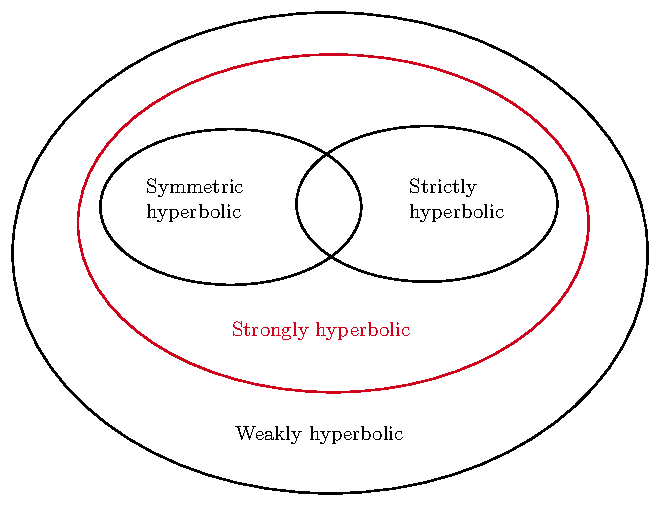
\includegraphics[width=0.5\textwidth]{tikz/weak-hyperbolic.pdf}
    \caption{双曲型问题几个定义之间的关系} \label{fig:weak-hyperbolic}
\end{figure}


\begin{theorem}\label{thm:well-posed-2}
    问题~\eqref{eq:1d-pdes-hyperbolic} 适定的充要条件为:PDEs 为强双曲问题。(弱双曲无法保证适定性)
\end{theorem}

\begin{proof}
    证明见下文。
\end{proof}

考虑带非导数项的问题
\begin{equation}
    \left\{
    \begin{aligned}
         & U_t = A\,U_x  + B\,U \\
         & U(x,0) = F(x)
    \end{aligned}
    \right.
    \label{eq:1d-pdes-hyperbolic-2}
\end{equation}

\begin{theorem}\label{thm:well-posed-3}
    问题~\eqref{eq:1d-pdes-hyperbolic-2} 适定的一个充分条件为:$U_t = A\,U_x$ 为强双曲问题。
\end{theorem}

\begin{proof}
    证明见下文。
\end{proof}

\subsection{抛物型方程组}


考虑一维常系数二阶方程组:周期函数 $U: \mathbb{R} \times \mathbb{R}^+ \to \mathbb{C}^{m}$,常系数矩阵 $A,B,C \in \mathbb{C}^{m \times m}$,满足的 PDEs 为
\begin{equation}
    \left\{
    \begin{aligned}
         & U_t = A\,u_{xx} + B\,U_x + C\,U =: P\,U \\
         & U(x,0) = F(x)
    \end{aligned}
    \right.
    \label{eq:1d-pdes-parabolic}
\end{equation}

\begin{definition}
    称方程组~\eqref{eq:1d-pdes-parabolic} 是抛物型的,如果存在常数 $\delta > 0$,使得 $A$ 的所有特征值 $\lambda$ 都满足 $\Re\, \lambda \ge \delta$。
\end{definition}


\begin{theorem}\label{thm:well-posed-4}
    抛物型问题是适定的。
\end{theorem}

\begin{proof}
    证明见下文。
\end{proof}

\section{一般常系数方程组的适定性}

考虑一般的问题:周期函数 $u: \mathbb{R}^d  \times \mathbb{R}^+ \to \mathbb{C}^{m}$,满足的 PDEs 为
\begin{equation}
    \left\{
    \begin{aligned}
         & u_t = P(\frac{\partial}{\partial x}) u \\
         & u(x,0) = f(x)
    \end{aligned}
    \right.
    \label{eq:pdes-general}
\end{equation}
这里的 $x \in \mathbb{R}^d$ 有多个分量,对应的 $\frac{\partial}{\partial x}$ 是在多重指标意义下的。
谐波解形如
\[
    \widehat{U}(\omega ,t) = e^{\widehat{P}(i \omega )t} \widehat{F}(\omega )
\]

\begin{remark}
    这里的记号 $e^M$ 是矩阵指数
    \[
        e^M = I + M + \frac{M^2}{2!} + \frac{M^3}{3!} + \cdots
    \]
\end{remark}

由于适定性要求对任意初值都成立,可以自然得到如下充要条件:
\begin{theorem}
    初值问题~\eqref{eq:pdes-general} 是适定的,等价于存在常数 $K,\alpha$,使得对于任意 $\omega $ 都有
    \[
        \| e^{\widehat{P}(i \omega )t} \| \le K e^{\alpha t}
    \]
\end{theorem}

这个充要条件不太实用,但是可以据此推出更好用必要或充分条件。
\begin{theorem}[The Petrovskii condition]
    初值问题~\eqref{eq:pdes-general} 适定的必要条件为:存在常数 $\alpha$,使得对于任意 $\omega $,$\widehat{P}(i \omega)$ 的任意特征值 $\lambda(\omega )$,都有
    \[
        \Re\, \lambda(\omega ) \le \alpha
    \]
\end{theorem}

\begin{proof}
    取 $\widehat{P}(i \omega)$ 的任意特征值 $\lambda(\omega )$ 以及对应的单位特征向量 $\phi(\omega )$,满足
    \[
        \widehat{P}(i \omega) \phi(\omega ) = \lambda(\omega ) \phi(\omega ),\quad \Rightarrow \quad e^{\widehat{P}(i \omega)t} \phi(\omega ) = e^{\lambda(\omega )t} \phi(\omega )
    \]
    利用适定性的充要条件可得
    \[
        \left\|e^{\lambda(\omega )t}\right\|  = \left\|e^{\lambda(\omega )t} \phi(\omega ) \right\|
        = \left\| e^{\widehat{P}(i \omega)t} \phi(\omega )\right\| \le K e^{\alpha t}
    \]
    这表明 $\left\|e^{\lambda(\omega )t}\right\|$ 的增长被控制,即实部 $\Re\, \lambda(\omega )$ 存在一致的上界。
\end{proof}

\begin{theorem}\label{thm:well-posed-5}
    初值问题~\eqref{eq:pdes-general} 适定的一个充分条件为:$\widehat{P}(i \omega)$ 始终可以相似对角化,记作
    \[
        \widehat{P}(i \omega) = S(\omega ) \Lambda(\omega ) S^{-1}(\omega ),\quad \forall\,\omega
    \]
    并且满足:
    \begin{enumerate}
        \item 对于相似对角化的变换矩阵 $S(\omega )$,存在与 $\omega $ 无关的常数 $K$,使得
              \[
                  \| S(\omega ) \| \| S^{-1}(\omega ) \| \le K,\quad \forall\,\omega
              \]
        \item (The Petrovskii condition)对于对角阵 $\Lambda(\omega )$,存在与 $\omega $ 无关的常数 $\alpha$,使得
              \[
                  \Re \,\Lambda(\omega ) \le \alpha I,\quad \forall\,\omega
              \]
    \end{enumerate}
\end{theorem}

\begin{proof}
    \[
        \left\| e^{\widehat{P}(i \omega )t} \right\| = \left\| e^{S(\omega ) \Lambda(\omega ) S^{-1}(\omega )t} \right\|
        =
        \left\|S(\omega ) e^{\Lambda(\omega ) t}S^{-1}(\omega ) \right\| \le \left\|S(\omega )\right\| \left\|e^{\Lambda(\omega ) t}\right\| \left\|S^{-1}(\omega ) \right\|
        \le K e^{\alpha t} \qedhere
    \]
\end{proof}


\section{半有界算子与适定性}

仍然考虑的是一般的常系数方程组~\eqref{eq:pdes-general}。

\begin{definition}
    称算子 $P$ 是 $L^2$ 内积意义下的半有界算子,如果 $P$ 满足:存在常数 $\alpha$,使得对任意光滑函数 $v(x)$ 都有
    \[
        (v,Pv)+(Pv,v) \le 2\alpha (v,v)
    \]
    或者等价于要求 $\widehat{P}$ 满足
    \[
        \widehat{P}(i \omega) + \widehat{P}^{\mathsf{H}}(i \omega) \le 2 \alpha I,\quad \forall\,\omega
    \]
\end{definition}

\begin{remark}
    $P$ 是半有界算子并不意味着 $P$ 自身是有界的。
\end{remark}


易知半有界算子可以直接推出问题的适定性:
\begin{theorem}\label{thm:well-posed-6}
    若 $P$ 是 $L^2$ 内积意义下的半有界算子,则问题~\eqref{eq:pdes-general} 是适定的,并且解满足
    \[
        \| u(x,t) \| \le e^{\alpha t} \| u(x,0) \|
    \]
\end{theorem}

\begin{proof}
    \[
        \frac{d}{dt} \left[ e^{-2\alpha  t}(u,u) \right]
        =e^{-2\alpha t}(\frac{d}{dt}(u,u)-2\alpha (u,u))
        = e^{-2 \alpha t}\left[(u ,P u) + (P u,u) - 2\alpha (u,u)\right] \le 0
    \]
    因此
    \begin{gather*}
        e^{-2\alpha t} \| u(x,t) \|^2 \le  \| u(x,0) \|^2 \\
        \| u(x,t) \| \le e^{\alpha t}\| u(x,0) \| \qedhere
    \end{gather*}
\end{proof}

\begin{remark}
    半有界算子只是适定性的充分不必要条件,即使(在当前范数意义下)不是半有界算子,问题也可能是适定的。
\end{remark}

我们还可以通过一个正定矩阵将半有界算子定义中的 $L^2$ 内积和范数进行推广:
考虑一个关于 $\omega $ 的正定矩阵 $\widehat{H}(\omega)$,
此时可以定义一个新的内积 $(\cdot,\cdot)_H$ 和范数 $\| \cdot \|_H$:
\[
    (v_1,v_2)_H := \sum_\omega \langle\hat{v}_1(\omega),\widehat{H}(\omega)\hat{v}_2(\omega)\rangle,\quad
    \| v \|_H := \sqrt{(v,v)_H}
\]
并且要求存在与 $\omega $ 无关的常数 $K>0$ 使得
\[
    \frac{1}{K}I \le \widehat{H}(\omega ) \le K I,\quad \forall\,\omega
\]
这实际是要求新内积和原本的 $L^2$ 内积是等价的。
原本的 $L^2$ 内积相当于选择了平凡的单位阵 $\widehat{H}(\omega ) = I$。

\begin{definition}
    称算子 $P$ 在 $H$ 内积意义下是半有界算子,如果满足存在常数 $\alpha$,使得对任意光滑函数 $v(x)$ 都有
    \[
        (v,Pv)_H + (Pv,v)_H \le 2\alpha (v,v)_H
    \]
    或者等价于要求 $\widehat{P}$ 满足
    \[
        \widehat{H}(\omega ) \widehat{P}(i \omega) + \widehat{P}^{\mathsf{H}}(i \omega) \widehat{H}(\omega ) \le 2\alpha \widehat{H}(\omega ),\quad \forall\,\omega
    \]
\end{definition}
同理可以证明:如果 $P$ 在 $H$ 内积意义下为半有界算子,那么原问题在 $H$ 范数意义下是适定的,
又因为范数等价,在 $L^2$ 范数意义下也是适定的。
利用不同范数意义下的半有界算子,可以得到如下的适定性充要条件:

\begin{theorem}\label{thm:well-posed-7}
    问题~\eqref{eq:pdes-general} 是适定的,等价于可以构造出合适的 $\widehat{H}(\omega )$,使得 $P$ 在 $H$ 内积的意义下为半有界算子,即:存在常数 $K,\alpha >0$,使得
    \begin{gather}
        \frac{1}{K}I \le \widehat{H}(\omega ) \le K I, \quad \forall\,\omega  \label{eq:well-posed-condition-1}\\
        \widehat{H}(\omega ) \widehat{P}(i \omega) + \widehat{P}^{\mathsf{H}}(i \omega) \widehat{H}(\omega ) \le 2\alpha \widehat{H}(\omega ),\quad \forall\,\omega \label{eq:well-posed-condition-2}
    \end{gather}
\end{theorem}


\section{一些定理的证明}

使用半有界算子理论可以简化几个定理的证明过程,因此将证明留在了最后。

\begin{proof}[\normalfont\bfseries Proof of Theorem~\ref{thm:well-posed-2}]
    证明分为如下几个步骤:
    \begin{enumerate}
        \item 首先假设问题~\eqref{eq:1d-pdes-hyperbolic} 是适定的,证明 $A$ 的特征值必须全为实数;
        \item 然后假设 $A$ 的特征值全部为实数,并且具有完备的特征系统,证明问题是适定的;
        \item 最后假设 $A$ 的特征值全部为实数,并且不具备完备的特征系统,证明问题是不适定的。
    \end{enumerate}

    不妨设 $A$ 的特征值为 $\lambda$,对应的特征向量为 $\phi$,满足 $A \phi = \lambda \phi$。
    取初值
    \[
        U(x,0) = e^{i \omega x} \phi.
    \]
    则精确解为
    \[
        U(x,t) = e^{i \omega (x + \lambda t)} \phi.
    \]
    因此
    \[
        \| U(x,t) \| = \| e^{i \omega (x + \lambda t)} \phi \| = e^{\Re(i \omega \lambda t)} \| U(x,0) \|.
    \]
    如果问题是适定的,则存在常数 $\alpha$ 使得
    \[
        \Re(i \omega \lambda t) \le \alpha,\quad \forall\, \omega
    \]
    这表明必然有 $\Im(\lambda) = 0$,即特征值 $\lambda$ 均为实数。

    假设 $A$ 的特征值全部为实数,并且具有完备的特征系统,即 $A$ 可以相似对角化
    \[
        A = S \Lambda S^{-1},\quad \Lambda = \text{diag}(\lambda_1, \cdots, \lambda_m),\quad \lambda_i \in \mathbb{R}.
    \]
    那么通过换元 $U = S V$ 可以得到
    \[
        U_t = A U_x = S \Lambda S^{-1} U_x, \quad \Rightarrow \quad V_t = \Lambda V_x.
    \]
    显然有
    \[
        \| V(x,t) \| = \| V(x,0) \|
    \]
    因此
    \[
        \| U(x,t) \| = \| S\,V(x,t) \| \le \| S \|\,\| V(x,t) \| = \| S \|\,\| V(x,0) \|
        \le  \| S \|\, \| S^{-1} \|\,\| U(x,0) \|
    \]

    最后说明 $A$ 具有完备的特征系统是必要的,通过反证法证明:假设 $A$ 是一个 Jordan 块
    \[
        A = \begin{bmatrix}
            \lambda & 1       &        &         \\
                    & \lambda & \ddots &         \\
                    &         & \ddots & 1       \\
                    &         &        & \lambda \\
        \end{bmatrix}
        = \lambda I + J,\quad \lambda \in \mathbb{R}.
    \]
    取初值
    \[
        U(x,0) = e^{i \omega x} \widehat{U}(\omega,0)
    \]
    则精确解为
    \[
        U(x,t) =  e^{i \omega (\lambda I + J) t} e^{i \omega x} \widehat{U}(\omega,0)
    \]
    因此
    \[
        \|U(x,t)\| \le \|e^{i \omega (\lambda I + J) t}\| \|U(\omega,0)\|
    \]
    问题是适定的等价于存在常数 $K,\alpha$,使得
    \[
        \|e^{i \omega (\lambda I + J) t}\| \le K e^{\alpha t},\quad \forall\,\omega
    \]
    但是注意到
    \[
        \left\| e^{i \omega (\lambda I + J) t} \right\|
        = \left\| e^{i \omega \lambda I t} \right\| \left\| e^{i \omega J t} \right\|
        = \left\| e^{i \omega J t} \right\|
        = \left\|
        \sum_{\ell=0}^{m-1} \frac{(i \omega t)^{\ell}}{\ell!} J^{\ell}
        \right\|
    \]
    显然不存在与 $\omega$ 无关的上界,因此问题不适定。

    综上可得,问题~\eqref{eq:1d-pdes-hyperbolic} 是适定的等价于 $A$ 的特征值全部为实数,并且具有完备的特征系统,即 PDEs 为强双曲问题。
\end{proof}

\begin{proof}[\normalfont\bfseries Proof of Theorem~\ref{thm:well-posed-3}]
    对于 $U_t = A U_x + B U$,由于$A$ 可以相似对角化
    \[
        A = S \Lambda S^{-1},\quad \Lambda = \text{diag}(\lambda_1, \cdots, \lambda_m),\quad \lambda_i \in \mathbb{R}.
    \]
    那么可以通过换元 $U = S V$ 得到
    \[
        U_t = A U_x + B U, \quad \Rightarrow \quad V_t = \Lambda V_x + \widetilde{B} V =: P V.\quad (\widetilde{B} := S^{-1} B S)
    \]
    转换为 Fourier 系数满足的方程组
    \[
        \widehat{V}_t = (i \omega \Lambda + \widetilde{B} S) \widehat{V} =: \widehat{P}(i \omega) \widehat{V}
    \]
    下面证明 $P$ 是半有界算子
    \[
        \widehat{P}(i \omega) + \widehat{P}^\mathsf{H}(i \omega)
        = (i \omega \Lambda + \widetilde{B}) + (- i \omega \Lambda + \widetilde{B}^\mathsf{H})
        = \widetilde{B} + \widetilde{B}^\mathsf{H}
        \le 2 \alpha I,\quad (\alpha = \|\widetilde{B}\|)
    \]
    因此 $V$ 满足
    \[
        \| V(x,t) \| \le e^{\alpha t} \| V(x,0) \|,
    \]
    换元得到 $U$ 满足
    \[
        \| U(x,t) \| = \| S V(x,t) \| \le e^{\alpha t}  \| S \| \| V(x,0) \|
        \le e^{\alpha t}  \| S \| \| S^{-1} \| \| U(x,0) \|
    \]
    因此如果 $U_t = A\,U_x$ 为强双曲问题,则方程~\eqref{eq:1d-pdes-hyperbolic-2} 是适定的。
\end{proof}

为了证明抛物型方程组问题的适定性,我们需要如下引理:
\begin{lemma}\label{lemma:well-posed-1}
    下面两个结论等价:
    \begin{enumerate}
        \item 存在常数 $\delta >0$,使得 $A$ 的所有特征值 $\lambda$ 都满足 $\Re\, \lambda \ge \delta$;
        \item 存在常数 $\delta' >0$ 以及正定矩阵 $H$,使得 $H A + A^{\mathsf{H}} H \ge \delta' H$。
    \end{enumerate}
\end{lemma}

\begin{proof}
    \noindent
    \begin{enumerate}
        \item 假设存在常数 $\delta >0$,使得 $A$ 的所有特征值 $\lambda$ 都满足 $\Re\, \lambda \ge \delta$。
              根据 Schur 引理,可以使用酉方阵 $U$ 将其上三角化
              \[
                  U^\mathsf{H} A U
                  = \begin{bmatrix}
                      \lambda_1 &           &        &        &           \\
                                & \lambda_2 &        &        &           \\
                                &           & \ddots &        &           \\
                                &           &        & \ddots &           \\
                                &           &        &        & \lambda_m
                  \end{bmatrix}
                  +
                  \begin{bmatrix}
                      0 & \tilde{a}_{12} & \cdots         & \cdots & \tilde{a}_{1m}     \\
                        & 0              & \tilde{a}_{23} & \ddots & \tilde{a}_{2m}     \\
                        &                & \ddots         & \ddots & \vdots             \\
                        &                &                & \ddots & \tilde{a}_{m-1\,m} \\
                        &                &                &        & 0
                  \end{bmatrix}
                  =: \Lambda + B
              \]
              定义对角阵 $D_\varepsilon$
              \[
                  D_\varepsilon := \text{diag}(1,\varepsilon,\dots,\varepsilon^{m-1}),\quad (\varepsilon > 0)
              \]
              则有
              \begin{align*}
                  D_\varepsilon^{-1} U^\mathsf{H} A U D_\varepsilon
                  ={} & D_\varepsilon^{-1} ( \Lambda + B ) D_\varepsilon    \\
                  ={} & \begin{bmatrix}
                            \lambda_1 &           &        &        &           \\
                                      & \lambda_2 &        &        &           \\
                                      &           & \ddots &        &           \\
                                      &           &        & \ddots &           \\
                                      &           &        &        & \lambda_m
                        \end{bmatrix}
                  +
                  \begin{bmatrix}
                      0 & \varepsilon \tilde{a}_{12} & \cdots                    & \cdots & \varepsilon^{m-1} \tilde{a}_{1m} \\
                        & 0                          & \varepsilon\tilde{a}_{23} & \ddots & \varepsilon^{m-2} \tilde{a}_{2m} \\
                        &                            & \ddots                    & \ddots & \vdots                           \\
                        &                            &                           & \ddots & \varepsilon \tilde{a}_{m-1\,m}   \\
                        &                            &                           &        & 0
                  \end{bmatrix}
                  \\
                  ={} & \Lambda + D_\varepsilon^{-1} B D_\varepsilon
              \end{align*}
              定义 $\widetilde{A}_\varepsilon = D_\varepsilon^{-1} U^\mathsf{H} A U D_\varepsilon$,显然 $\widetilde{A}_\varepsilon$ 与 $A$ 的特征值相同,并且有
              \[
                  \widetilde{A}_\varepsilon + \widetilde{A}^{\mathsf{H}}_\varepsilon
                  ={}  2 \Re(\Lambda) + D_\varepsilon^{-1} B D_\varepsilon + D_\varepsilon^{\mathsf{H}} B^{\mathsf{H}} D_\varepsilon^{-\mathsf{H}}
                  \ge{}  2 \delta I + D_\varepsilon^{-1} B D_\varepsilon + D_\varepsilon^{\mathsf{H}} B^{\mathsf{H}} D_\varepsilon^{-\mathsf{H}}
              \]
              由于 $\|D_\varepsilon^{-1} B D_\varepsilon\| = \mathcal{O}(\varepsilon)$,
              显然存在 $\varepsilon_0 > 0$,使得当$ 0 < \varepsilon < \varepsilon_0$ 足够小时
              \[
                  \widetilde{A}_\varepsilon + \widetilde{A}^{\mathsf{H}}_\varepsilon \ge \delta I.
              \]
              因此
              \begin{gather*}
                  (U D_\varepsilon)^{-\mathsf{H}} (\widetilde{A}_\varepsilon + A^{\mathsf{H}}_\varepsilon) (U D_\varepsilon)^{-1} \ge \delta\,(U D_\varepsilon)^{-\mathsf{H}} (U D_\varepsilon)^{-1}.
                  \\
                  (U D_\varepsilon)^{-\mathsf{H}} (U D_\varepsilon)^{-1} A + A^{\mathsf{H}} (U D_\varepsilon)^{-\mathsf{H}} (U D_\varepsilon)^{-1} \ge \delta\,(U D_\varepsilon)^{-\mathsf{H}} (U D_\varepsilon)^{-1}.
              \end{gather*}
              取 $H = (U D_\varepsilon)^{-\mathsf{H}} (U D_\varepsilon)^{-1}$ 即可完成证明。
        \item 假设存在常数 $\delta' >0$ 以及正定矩阵 $H$,使得 $H A + A^{\mathsf{H}} H \ge \delta' H$,
              那么对于 $A$ 的任意特征值 $\lambda$ 以及对应的特征向量 $v$,有
              \[
                  0 \le v^{\mathsf{H}} (H A + A^{\mathsf{H}} H - \delta' H) v =  (2 \Re(\lambda) - \delta') v^{\mathsf{H}} H v
              \]
              因此任意特征值均满足 $\Re(\lambda) \ge \frac12\delta'$。
    \end{enumerate}
\end{proof}

\begin{remark}
    上述引理的第一条对应The Petrovskii condition,第二条则对应定理~\ref{thm:well-posed-7} 的条件~\eqref{eq:well-posed-condition-2},
    只是因为二阶导使得不等号全部取反。
\end{remark}

\begin{remark}
    无法通过 $\Re(\lambda(A)) \ge \delta$ 直接推出
    \[
        \exists\,\,\delta' > 0,\quad \text{s.t.} \quad A + A^{\mathsf{H}} \ge \delta' I
    \]
    可以给出一个反例,考虑
    \[
        A = \begin{bmatrix}
            1 & 4 \\
            0 & 1
        \end{bmatrix},\quad  A + A^{\mathsf{H}} = \begin{bmatrix}
            2 & 4 \\
            4 & 2
        \end{bmatrix}
    \]
    $A$ 满足要求,但是 $A + A^{\mathsf{H}}$ 不是正定矩阵。
    但是可以构造合适的 $H$ 满足引理中的要求,例如
    \[
        H = \begin{bmatrix}
            1 & 1 \\
            1 & 6
        \end{bmatrix}, \quad
        H A + A^{\mathsf{H}} H = \begin{bmatrix}
            2 & 6  \\
            6 & 20
        \end{bmatrix} > \frac{1}{10} H
    \]
\end{remark}

\begin{proof}[\normalfont\bfseries Proof of Theorem~\ref{thm:well-posed-4}]
    对于方程组
    \[
        U_t = A U_{xx} + B U_x + C U =: P U
    \]
    转换为 Fourier 系数满足的方程组
    \[
        \widehat{U}_t = (i \omega)^2 A \widehat{U}  + (i \omega) B \widehat{U} + C \widehat{U}
        =: \widehat{P}(i \omega) \widehat{U}
    \]
    由于 PDEs 为抛物型问题,根据引理~\ref{lemma:well-posed-1},存在正定矩阵 $H$ 以及 $\delta > 0$,使得
    \[
        H A + A^\mathsf{H} H \ge \delta H.
    \]
    因此
    \begin{align*}
        H \widehat{P}(i \omega) + \widehat{P}^\mathsf{H}(i \omega) H
        ={}   & \left(-\omega^2 H A + i \omega H B + H C\right)
        + \left(-\omega^2 A^\mathsf{H} H - i \omega B^\mathsf{H} H + C^\mathsf{H} H\right)                \\
        ={}   & -\omega^2 (H A + A^\mathsf{H} H) + i \omega (H B - B^\mathsf{H}H) + (HC + C^\mathsf{H} H) \\
        \le{} & - 2 \delta\, \omega^2 H + i \omega (H B - B^\mathsf{H}H) + (HC + C^\mathsf{H} H)
    \end{align*}
    因为关于 $\omega$ 的二次项系数为负,显然存在与 $\omega$ 无关的有限上界 $\alpha > 0$,使得
    \[
        H \widehat{P}(i \omega) + \widehat{P}^\mathsf{H}(i \omega) H \le 2 \alpha H
    \]
    利用定理~\ref{thm:well-posed-7} 即可证明问题的适定性。
\end{proof}


\section{一些例子}

\begin{example}
    考虑如下偏微分方程组
    \[
        u_t = A u_x + B u,
    \]
    矩阵 $A$, $B$ 在满足何种条件时可以保证能量守恒?(即 $\|u(x,t)\| = \|u(x,0)\|$)
\end{example}

\begin{solution*}
    考虑谐波解
    \[
        u(x,t) = e^{i \omega x} \hat{u}(\omega,t),\quad
        u(x,0) = e^{i \omega x} \hat{f}(\omega)
    \]
    代入方程得到
    \[
        \left\{
        \begin{aligned}
             & \hat{u}_t = (i \omega A + B) \hat{u}, \\
             & \hat{u}(\omega,0) = \hat{f}(\omega)
        \end{aligned}
        \right.
        \quad \Rightarrow \quad
        \hat{u}(\omega,t) = e^{(i \omega A + B)t}\hat{f}(\omega)
    \]
    能量守恒即
    \[
        \| u(x,t) \|^2 =\| u(x,0) \|^2, \quad
        \iff \quad |\hat{u}( \omega,t)|^2 = |\hat{u}( \omega,0)|^2
    \]
    对时间求导
    \begin{align*}
        \partial_t |\hat{u}( \omega,t)|^2
         & = (\hat{u},\hat{u}_t) + (\hat{u}_t,\hat{u})                               \\
         & = (\hat{u},(i \omega A + B) \hat{u}) + ((i \omega A + B) \hat{u},\hat{u}) \\
         & = (\hat{u},(i \omega (A - A^\mathsf{H}) + (B + B^\mathsf{H}))\hat{u})
    \end{align*}
    因此当 $A=A^\mathsf{H}$,$B+B^\mathsf{H}=0$ 时,$\partial_t |\hat{u}( \omega,t)|^2=0$,能量守恒。
\end{solution*}

\begin{example}\label{eg:well-posed-1}
    求证:对于抛物型方程组 $u_t = A u_{xx}$,存在常数 $\delta > 0$ 和 $K > 0$,使得
    \[
        \| u(x,t) \|^2 + \delta \int_0^t \| u_x(x,\xi) \|^2 \,d\xi \le K \| u(x,0) \|^2
    \]
\end{example}

\begin{solution*}
    易知对于抛物方程,存在 $\delta' >0$ 和正定矩阵 $H$ 使得 $H A + A^\mathsf{H} H \ge \delta' H$,
    定义 $H$ 内积以及对应的 $H$ 范数
    \[
        (v_1,v_2)_H := \sum_\omega \langle\hat{v}_1(\omega),H \hat{v}_2(\omega)\rangle
    \]
    显然两个范数是等价的:存在 $C>0$ 使得
    \[
        \frac{1}{C} \| u \|_H^2  \le \| u \|^2 \le C \| u \|_H^2,
    \]

    考虑谐波解
    \[
        u(x,t) = e^{i \omega x} \hat{u}(\omega,t),\quad
        u(x,0) = e^{i \omega x} \hat{f}(\omega)
    \]
    代入方程得到
    \[
        \left\{
        \begin{aligned}
             & \hat{u}_t = (i \omega)^2 A \hat{u}, \\
             & \hat{u}(\omega,0) = \hat{f}(\omega)
        \end{aligned}
        \right.
        \quad \Rightarrow \quad
        \hat{u}(\omega,t) = e^{- \omega^2 A t}\hat{f}(\omega)
    \]
    易得
    \begin{gather*}
        \| u(x,t) \|^2 = \hat{u}^\mathsf{H}(\omega,t) \hat{u}(\omega,t),\quad
        \| u_x(x,t) \|^2 = \omega^2 \hat{u}^\mathsf{H}(\omega,t) \hat{u}(\omega,t), \\
        \| u(x,t) \|_H^2 = \hat{u}^\mathsf{H}(\omega,t) H \hat{u}(\omega,t),\quad
        \| u_x(x,t) \|_H^2 = \omega^2 \hat{u}^\mathsf{H}(\omega,t) H \hat{u}(\omega,t).
    \end{gather*}
    对$\| u(x,t) \|_H^2$关于时间求导
    \begin{align*}
        \partial_t \| u(x,t) \|_H^2
        ={}   & \hat{u}_t^\mathsf{H}(\omega,t) H \hat{u}(\omega,t) + \hat{u}^\mathsf{H}(\omega,t) H \hat{u}_t(\omega,t) \\
        ={}   & - \omega^2 \hat{u}^\mathsf{H}(\omega,t) (A^\mathsf{H} H + H A) \hat{u}(\omega,t)                        \\
        \le{} & - \omega^2 \delta' \hat{u}^\mathsf{H}(\omega,t) H \hat{u}(\omega,t).
    \end{align*}
    因此
    \[
        \partial_t \| u(x,t) \|_H^2 + \omega^2 \delta'\, \hat{u}^\mathsf{H}(\omega,t) H \hat{u}(\omega,t) \le 0
    \]
    对时间积分可得
    \[
        \| u(x,t) \|_H^2  +\omega^2  \delta' \int_0^t \hat{u}^\mathsf{H}(\omega,\xi) H \hat{u}(\omega,\xi) \,d\xi \le \| u(0,t) \|_H^2
    \]
    再利用范数等价性可得
    \[
        \| u(x,t) \|^2  + \delta' \int_0^t \| u_x(x,t) \|^2 \,d\xi \le C^2 \| u(0,t) \|^2
    \]
    取 $K=C^2$,$\delta = \delta'$ 即可得证。
\end{solution*}

\begin{example}
    考虑含低阶项的抛物型方程组
    \[
        u_t = A u_{xx} + B u_x + C u
    \]
    其中 $B$ 是 Hermite 矩阵, $C$ 是反 Hermite 矩阵。
    那么例~\ref{eg:well-posed-1} 中的不等式是否仍然成立?
    \[
        \| u(x,t) \|^2 + \delta \int_0^t \| u_x(x,\xi) \|^2 \,d\xi \le K \| u(x,0) \|^2
    \]
\end{example}

\begin{proof}
    方程 $v_t = A v_{xx}$ 的解 $v$ 满足
    \begin{align*}
        \partial_t \| v(x,t) \|^2
        ={} & \hat{v}_t^\mathsf{H}(\omega,t) \hat{v}(\omega,t) + \hat{v}^\mathsf{H}(\omega,t) \hat{v}_t(\omega,t) \\
        ={} & - \omega^2 \hat{v}^\mathsf{H}(\omega,t) (A^\mathsf{H} + A) \hat{v}(\omega,t).
    \end{align*}
    方程 $u_t = A u_{xx} + B u_x + C u$ 的解 $u$ 满足
    \begin{align*}
        \partial_t \| u(x,t) \|^2
        ={} & \hat{u}_t^\mathsf{H}(\omega,t) \hat{u}(\omega,t) + \hat{u}^\mathsf{H}(\omega,t) \hat{u}_t(\omega,t) \\
        ={} & - \omega^2 \hat{u}^\mathsf{H}(\omega,t) (A^\mathsf{H} + A) \hat{u}(\omega,t)
        - i \omega \hat{u}^\mathsf{H}(\omega,t) (B^\mathsf{H} - B) \hat{u}(\omega,t)                              \\
            & + \hat{u}^\mathsf{H}(\omega,t)(C^\mathsf{H} + C) \hat{u}(\omega,t)                                  \\
        ={} & - \omega^2 \hat{u}^\mathsf{H}(\omega,t) (A^\mathsf{H} + A) \hat{u}(\omega,t).
    \end{align*}
    因此如果对两个方程组选取相同的初值,就有
    \[
        \| u(x,t) \| = \| v(x,t) \|,\quad \forall\, t \ge 0
    \]
    同理
    \[
        \| u_x(x,t) \| = \| v_x(x,t) \|,\quad \forall\, t \ge 0
    \]
    因此原本的估计仍然成立。
\end{proof}

下面提供几个半有界算子的例子。

\begin{example}
    考虑如下偏微分方程组
    \[
        u_t = (A(x,t) u_x)_x =: P u
    \]
    其中矩阵 $A(x,t)$ 关于 $x$ 有周期性,并且满足 $A + A^{\mathsf{H}}$ 的特征值有一致下界 $\delta > 0$,那么 $P$ 是半有界算子。
\end{example}

\begin{proof}
    \begin{align*}
        (u, P u) + (P u, u) ={} & (u, (A u_x)_x) + ((A u_x)_x, u)
        \\
        ={}                     & -(u_x, A u_x) - (A u_x, u_x)    \\
        ={}                     & -(u_x, (A+A^{\mathsf{H}})u_x)   \\
        \le                     & -\delta \, \|u_x\|_2^2 \le 0
    \end{align*}
    取 $\alpha = 0$ 即可满足要求。
\end{proof}

\begin{example}
    考虑如下偏微分方程组
    \[
        u_t = B u_x + C u =: P u
    \]
    其中常系数矩阵 $B,C$,并且 $B$ 是 Hermite 矩阵,那么 $P$ 是半有界算子。
\end{example}

\begin{proof}
    \begin{align*}
        (u, P u) + (P u, u) ={} & (u, B u_x) + (B u_x, u) + (u, C u) + (C u, u)                  \\
        ={}                     & (u, B u_x) -(u, B^{\mathsf{H}} u_x) + (u, (C+C^{\mathsf{H}})u) \\
        ={}                     & (u, (C+C^{\mathsf{H}})u)                                       \\
        \le                     & 2 \| C \| \, \|u\|_2^2
    \end{align*}
    取 $\alpha = \| C \|$ 即可满足要求。
\end{proof}

\begin{example}
    考虑如下偏微分方程组
    \[
        u_t=
        \begin{bmatrix}
            1 & 10 \\
            0 & 2
        \end{bmatrix} u_x.
    \]
    构造合适的 $\widehat{H}(\omega)$,使得 $P$ 在 $H$ 内积意义下为半有界算子,从而利用定理~\ref{thm:well-posed-7} 证明方程组的适定性。
\end{example}

\begin{solution*}
    代入谐波解可以得到
    \[
        \widehat{P}(i\omega)=i\omega \begin{bmatrix}
            1 & 10 \\
            0 & 2
        \end{bmatrix},\quad
        \widehat{P}^\mathsf{H}(i\omega)=-i\omega \begin{bmatrix}
            1  & 0 \\
            10 & 2
        \end{bmatrix}
    \]
    假设 Hermite 矩阵 $\widehat{H}(\omega) = \widehat{H}$ 与 $\omega$ 无关,形如
    \[
        \widehat{H}(\omega)=\begin{bmatrix}
            a       & c \\
            \bar{c} & b
        \end{bmatrix}
    \]
    其中常数 $a,b \in \mathbb{R}$,$c \in \mathbb{C}$。
    此时条件~\eqref{eq:well-posed-condition-1} 等价于要求 $\widehat{H}$ 正定,即两个特征值严格大于0,具体即
    \[
        a > 0,\quad b > 0,\quad a b > |c|^2
    \]
    接下来处理条件~\eqref{eq:well-posed-condition-2}
    \begin{gather*}
        \widehat{H}(\omega)\widehat{P}(i\omega)+\widehat{P}^\mathsf{H}(i\omega)\widehat{H}=
        i\omega \begin{bmatrix}
            0            & 10a+c         \\
            -10a-\bar{c} & 10(\bar{c}-c)
        \end{bmatrix} \\
        2 \alpha \widehat{H} - \left[\widehat{H}(\omega)\widehat{P}(i\omega)+\widehat{P}^\mathsf{H}(i\omega)\widehat{H}\right]
        = \begin{bmatrix}
            2 \alpha a                                   & 2 \alpha c - i \omega(10 a + c)     \\
            2 \alpha \bar{c} + i \omega (10 a + \bar{c}) & 2 \alpha b + i \omega (c - \bar{c})
        \end{bmatrix} =: A
    \end{gather*}
    因此条件~\eqref{eq:well-posed-condition-2} 要求上述矩阵 $A$ 半正定,这等价于要求 $2 \alpha a \ge 0$ 以及
    \[
        \text{det}(A) = 2 \alpha a(2 \alpha b + 10 i \omega(c - \bar{c}))
        - |2\alpha c - i \omega(10a + c)|^2 \ge 0,\quad \forall \omega
    \]
    这个式子是关于 $\omega$ 的实值二次函数,并且二次项系数非正,因此 $\text{det}(A) \ge 0$ 恒成立要求二次项系数严格为0,即
    \[
        10 a + c = 0, \quad \Rightarrow \quad c = -10 a \in \mathbb{R}
    \]
    此时条件变为$\text{det}(A) = 4 \alpha^2 (a b - c^2) \ge 0$,在 $ab > |c|^2$ 时自动成立。


    整理上述所有条件可得
    \[
        a > 0,\quad c = -10 a,\quad b > 100 a.
    \]
    例如可以取 $a=1$,$c = -10$,$b = 200$,构造$\widehat{H}(\omega)=\widehat{H}$为
    \[
        \widehat{H}(\omega)=\widehat{H}=\begin{bmatrix}
            1   & -10 \\
            -10 & 200
        \end{bmatrix}
    \]
    取 $\alpha = 0$ 即可满足~\eqref{eq:well-posed-condition-2}。
    条件~\eqref{eq:well-posed-condition-1} 要求存在 $K > 0$ 使得
    \begin{align*}
        \widehat{H}(\omega)-K^{-1}I & =
        \begin{bmatrix}
            a - \frac{1}{K} & c              \\
            \bar{c}         & b -\frac{1}{K}
        \end{bmatrix}
        =
        \begin{bmatrix}
            1 - \frac{1}{K} & -10              \\
            -10             & 200 -\frac{1}{K}
        \end{bmatrix}
        \ge 0
        \\
        K I-\widehat{H}(\omega)     & =
        \begin{bmatrix}
            K - a    & -c  \\
            -\bar{c} & K-b
        \end{bmatrix}
        =
        \begin{bmatrix}
            K - 1 & 10    \\
            10    & K-200
        \end{bmatrix}
        \ge 0
    \end{align*}
    取足够大的$K$即可满足,例如$K=201$。
\end{solution*}

\begin{remark}
    直接计算 $\widehat{P}(i\omega) + \widehat{P}^\mathsf{H} (i\omega)$ 可得
    \[
        \widehat{P}(i\omega) + \widehat{P}^\mathsf{H} (i\omega) = i \omega
        \begin{bmatrix}
            0 & 10 \\ -10 & 0
        \end{bmatrix}
        =
        \left(\frac{1}{\sqrt{2}}
        \begin{bmatrix}
            -i & i \\ 1 & 1
        \end{bmatrix}\right)
        \begin{bmatrix}
            -10 \omega & \\  & 10 \omega
        \end{bmatrix}
        \left(
        \frac{1}{\sqrt{2}}
        \begin{bmatrix}
            -i & i \\ 1 & 1
        \end{bmatrix}
        \right)^\mathsf{H}
    \]
    因此不存在常数 $\alpha \in \mathbb{R}$ 使得下式成立
    \[
        \widehat{P}(i \omega) + \widehat{P}^\mathsf{H} (i \omega) \le 2\alpha I
    \]
    这表明在 $L^2$ 内积意义下,$P$ 不是半有界算子,不能直接利用定理~\ref{thm:well-posed-6} 证明适定性,
    这同时也表明定理~\ref{thm:well-posed-6} 是适定性的充分不必要条件。
\end{remark}

\begin{remark}
    还可以利用定理~\ref{thm:well-posed-5} 证明该问题的适定性:计算可得 $\widehat{P}(i\omega)$ 的特征值为 $\lambda_1 = i \omega$,$\lambda_2 = 2 i \omega$,始终可以相似对角化
    \[
        \widehat{P}(i\omega) = i \omega
        \begin{bmatrix}
            1 & 10 \\ 0 & 2
        \end{bmatrix}
        =
        \begin{bmatrix}
            10 & 1 \\ 1 & 0
        \end{bmatrix}
        \begin{bmatrix}
            2 i \omega & \\ &  i \omega
        \end{bmatrix}
        \begin{bmatrix}
            10 & 1 \\ 1 & 0
        \end{bmatrix}^{-1}
        = S(\omega) \Lambda(\omega) S(\omega)^{-1}
    \]
    由于 $S(\omega)$ 与 $\omega$ 无关,显然存在常数 $K$ 使得 $\| S(\omega) \| \| S^{-1}(\omega) \| \le K$。
    由于特征值全部为纯虚数,$\Re \Lambda(\omega) = 0$ 满足 The Petrovskii condition。
    定理~\ref{thm:well-posed-5} 的三个条件全部满足,因此该问题是适定的。
\end{remark}


\chapter{差分方法的性质}

主要关注差分格式的三大性质:
\begin{itemize}
    \item 相容性:当网格尺寸趋于零时,差分格式应逼近于偏微分方程;
    \item 稳定性:偏微分方程的定解条件(初值,边值)的微小变化对差分格式的近似解的影响(在某个模的意义下)不应无限增长;(同理计算过程中的舍入误差也不会无限增长)
    \item 收敛性:当网格尺寸趋于零时,满足差分格式的近似解应收敛于满足偏微分方程的准确解。
\end{itemize}
此外,本章也关注偏微分方程和差分格式的耗散色散性分析。

\section{相容性}

相容性体现的是差分格式对偏微分方程的逼近程度,包括逐点相容性和模相容性,逐点相容性主要通过局部截断误差来衡量。

\begin{definition}[局部截断误差]
    对于偏微分方程 $\mathcal{L} u = g$ 以及对应的差分格式 $L v_j^n = g_j^n$,
    定义在 $(x_j,t^n)$ 处的局部截断误差为
    \[
        \tau_j^n := L u_j^n - g_j^n - (\mathcal{L}u(x_j,t^n) - g(x_j,t^n)) = L u_j^n - g_j^n
    \]
    其中 $u(x,t)$ 是满足偏微分方程的充分光滑函数。
\end{definition}

\begin{definition}[逐点相容性]
    称偏微分方程 $\mathcal{L} u = g$ 对应的差分格式 $L v_j^n = g_j^n$ 是(无条件)逐点相容的:如果局部截断误差 $\tau_j^n$ 在
    $\Delta x,\Delta t\to 0$时满足
    \[
        \tau_j^n \to 0.
    \]
    进一步,称这个格式的局部截断误差阶是 $(p,q)$ :如果存在不可改善的正数 $p,q$,使得下式成立
    \[
        \tau_j^n = \mathcal{O}((\Delta x)^p + (\Delta t)^q)
    \]
\end{definition}

\begin{remark}
    这里记号 $(p,q)$ 的分量顺序没有什么意义,在不同的资料中可能使用了不同的顺序,保持上下文记号一致即可。
\end{remark}

\begin{definition}[模相容性]\label{def:consistency-norm}
    对于双层差分格式
    \[
        V^{n+1} = Q \, V^{n} + \Delta t\, G^{n}
    \]
    将满足偏微分方程的充分光滑函数 $U$ 代入会产生余项 $\Delta t\,T^{n}$
    \[
        U^{n+1} = Q \, U^{n} + \Delta t\, G^{n} + \Delta t\, T^{n}
    \]
    称双层差分格式是(无条件)关于 $\|\cdot\|$ 模相容的:
    如果随着 $\Delta x \to 0$,$\Delta t \to 0$,有
    \[
        \|T^{n}\|  \to 0
    \]
    进一步,称这个格式的$\|\cdot\|$ 模相容阶是 $(p,q)$:如果存在不可改善的正数 $p,q$,使得下式成立
    \[
        \|T^{n}\|  = \mathcal{O}((\Delta x)^p + (\Delta t)^q)
    \]
\end{definition}

\begin{remark}
    对于显格式,通常可以整理为如下形式
    \[
        V^{n+1} = Q \, V^{n} + \Delta t\, G^{n}
    \]
    但是对于隐格式(例如全隐格式,Crank–Nicolson 格式,$\theta$ 格式),可能会得到如下形式
    \[
        P V^{n+1} = Q \, V^{n} + \Delta t\, G^{n}
    \]
    不需要计算 $P^{-1}$ 来整理为定义~\ref{def:consistency-norm} 中的形式,
    直接将满足偏微分方程的充分光滑函数 $U$ 代入会产生余项 $\Delta t\,T^{n}$
    \[
        P U^{n+1} = Q \, U^{n} + \Delta t\, G^{n} + \Delta t\, T^{n}
    \]
    相容性分析仍然是针对 $T^{n}$ 进行的。
\end{remark}

\section{稳定性}

稳定性体现的是偏微分方程的定解条件(初值,边值)的微小变化对差分格式的近似解的影响(在某个模的意义下),我们主要讨论初值稳定性。

\begin{definition}[稳定性]
    对于双层差分格式
    \[
        V^{n+1} = Q \, V^n,\quad n \ge 0,
    \]
    其中 $Q$ 为差分算子,$V^n = (\cdots,v_{-1}^n,v_0^n,v_1^n,\cdots)$。
    称该差分格式是关于 $\| \cdot \|$ 模稳定的,若对于任意 $(x,t)$,存在 $\Delta x_0 >0$,$\Delta t_0 > 0$,$K \ge 0$,$\beta \ge 0$,使得
    $\forall\, 0 < t = (n+1)\Delta t$,$0 < \Delta x \le \Delta x_0$,$0 < \Delta t \le \Delta t_0$,有
    \[
        \| V^{n+1} \| \le K e^{\beta t}\,\| V^0 \|
    \]
\end{definition}

\begin{remark}
    由于稳定性含义与具体的模选取有关,对同一个格式选择不同的模进行分析,也可能得到不同的稳定性结论。
\end{remark}

\begin{theorem}
    双层差分格式 $V^{n+1} = Q \, V^n$ 关于 $\| \cdot \|$ 模稳定的充要条件是:存在 $\Delta x_0 >0$,$\Delta t_0 > 0$,$K \ge 0$,$\beta \ge 0$,使得
    $\forall\, 0 < t = (n+1)\Delta t$,$0 < \Delta x \le \Delta x_0$,$0 < \Delta t \le \Delta t_0$,有
    \[
        \| Q^{n+1} \| \le K e^{\beta t}
    \]
\end{theorem}

\begin{theorem}
    双层差分格式 $V^{n+1} = Q \, V^n$ 关于 $\|\cdot\|$ 模稳定的必要条件是:
    存在常数 $C \ge 0$,使得
    \[
        \sigma(Q) = \max_i|\lambda_i(Q)| \le 1 + C\,\Delta t
    \]
\end{theorem}

\begin{remark}
    对于任意矩阵和任意范数,都有 $\sigma(A) \le \|A\|$ 成立,但是反方向的估计需要加上一些条件,这是上述命题通常只是必要而不充分的主要原因,
    例如:若 $Q$ 是正规矩阵(即 $Q Q^\mathsf{H} = Q^\mathsf{H} Q$),则上述条件是充要的。
    充分性证明利用了正规矩阵的性质 $\sigma(Q) = \| Q \|$;
    若 $Q$ 可以相似变换为一个正规矩阵:$Q = S \tilde{Q} S^{-1}$,并且变换矩阵及其逆矩阵的范数一致有界,那么也可以保证充分性,
    这利用了如下性质
    \[
        \| Q^n \| \le \| S \| \| S^{-1} \| \| \tilde{Q}^n \| = \| S \| \| S^{-1} \|\, |\sigma(Q)|^n
    \]
\end{remark}


\section{收敛性}

收敛性体现的是满足差分格式的近似解和满足偏微分方程的准确解之间的关系,包括逐点收敛和按模收敛。


\begin{definition}[逐点收敛性]
    称差分格式是(无条件)逐点收敛的,如果随着 $\Delta x,\,\Delta t \to 0$,
    $j\Delta x \to x_*$,$n \Delta t \to t_*$,有
    \[
        v_j^n \to u(x_*,t_*)
    \]
    其中 $u$ 是满足偏微分方程的充分光滑函数。
    进一步,称这个格式的逐点收敛阶为 $(p,q)$ :如果存在不可改善的正数 $p,q$,使得下式成立
    \[
        u(x_*,t_*) - v_j^n = \mathcal{O}((\Delta x)^p + (\Delta t)^q)
    \]
\end{definition}

\begin{definition}[模收敛性]
    称差分格式是(无条件)按$\| \cdot \|$ 模收敛的,如果随着 $\Delta x,\,\Delta t \to 0$,
    $n \Delta t \to t_*$,有
    \[
        \|U^n - V^n\| \to 0
    \]
    其中 $U$ 是满足偏微分方程的充分光滑函数。
    进一步,称这个格式在$\|\cdot\|$ 模意义下的收敛阶为 $(p,q)$ :如果存在不可改善的正数 $p,q$,使得下式成立
    \[
        \|U^n - V^n\| = \mathcal{O}((\Delta x)^p + (\Delta t)^q)
    \]
\end{definition}

\begin{remark}
    关于差分格式的精度,有的资料中将其视作格式的相容阶,有的资料中将其视作格式的收敛阶,
    虽然根据 Lax 等价定理,这两者通常是一致的,但是为了避免歧义,在笔记中选择避免使用精度的概念。
\end{remark}

\section{Lax 定理}

收敛性是我们的最终目标,但是不易证明,差分格式的相容性相对最容易验证。
基于Lax等价定理,可以将问题归结于差分格式的稳定性证明。

\begin{theorem}[Lax 等价定理]
    考虑一个适定的线性偏微分方程定解问题,若双层线性差分格式是相容的,那么它的稳定性与收敛性是等价的,并且收敛阶不低于相容阶。
\end{theorem}

\begin{remark}
    Lax 等价定理的充分性证明比较简单,但是必要性证明较为复杂,需要利用泛函分析中的共鸣定理。
\end{remark}

\begin{theorem}[Lax 定理]
    考虑一个适定的线性偏微分方程定解问题,假设它的双层线性差分格式
    \[
        V^{n+1} = Q \,V^n +\Delta t \,G^n
    \]
    是按 $\|\cdot\|$ 模相容的,并且关于 $\|\cdot\|$ 模具有 $(p,q)$ 阶相容阶,那么:
    格式若关于 $\|\cdot\|$ 模是稳定的,则关于 $\|\cdot\|$ 模 $(p,q)$ 阶收敛。
\end{theorem}

因此通常有两类方法可以证明格式的收敛性:
\begin{enumerate}
    \item 直接证明:先计算局部截断误差,然后计算整体误差 $e_j^n = u_j^n - v_j^n$,使用不等式放缩证明整体误差趋于0;
    \item 间接证明:分别证明相容性和稳定性,然后利用 Lax 等价定理得证收敛性。
\end{enumerate}

\section{稳定性证明}

根据 Lax 等价定理,我们主要关注格式的稳定性分析即可。
对于差分格式的稳定性证明有很多种方法,主要包括
\begin{enumerate}
    \item Fourier 方法($L^2$ 模稳定的充要条件)
    \item CFL 方法(任意模稳定的必要条件)
    \item 冻结系数法(稳定的必要条件)
    \item 离散最大模原理($L^\infty$ 模稳定的充分条件)
    \item 能量方法($L^2$ 模稳定的充分条件)
    \item[] $\cdots$
\end{enumerate}


\subsection{Fourier 方法}

对于纯初值问题或具有周期边界条件的问题,假设在空间上进行均匀剖分,考虑标量方程的线性常系数双层差分格式
\[
    V^{n+1} = Q \, V^n,\quad \widehat{V}^{n+1} = \widehat{Q} \, \widehat{V}^n
\]
记 $\widehat{Q}(\omega)$ 为放大因子,稳定性要求
\[
    \| V^{n+1}\|\le K e^{\beta(n+1)\Delta t} \,\| V^0\|
\]
其中 $K,\beta$ 是与时间无关的系数,$L^2$ 模稳定等价于要求
\[
    |\widehat{Q}(\omega)|^{n+1} \le K e^{\beta(n+1)\Delta t}
\]
由此可以导出著名的 von Neumann 条件。

\begin{theorem}[von Neumann condition]
    双层差分格式 $V^{n+1} = Q \, V^n$ 是 $L^2$ 模稳定的,等价于存在常数 $C>0$,使得放大因子 $\widehat{Q}(\omega)$ 在 $\Delta t$ 适当小的时候满足
    \[
        |\widehat{Q}(\omega)| \le 1+C \Delta t
    \]
\end{theorem}

\begin{proof}
    如果 $|\widehat{Q}(\omega)| \le 1 + C \Delta t$,根据不等式易得
    \[
        |\widehat{Q}(\omega)|^{n+1} \le (1 + C \Delta t)^{n+1} \le e^{C (n+1)\Delta t}.
    \]
    如果稳定,则有 $|\widehat{Q}(\omega)|  \le K^{\frac{1}{n+1}} e^{\beta \Delta t}$,也可以根据不等式进行放缩:
    记 $T = (n+1)\Delta t$,在 $\Delta t$ 足够小时成立
    \[
        |\widehat{Q}(\omega)|  \le K^{\frac{1}{n+1}} e^{\beta \Delta t}
        = K^{\frac{\Delta t}{T}} e^{\beta \Delta t}
        = e^{(\beta + \frac{\ln K}{T})\Delta t}
        = 1 + \mathcal{O}(\Delta t)
    \]
    因此,存在 $\Delta t_0$ 以及 $C>0$,使得对于 $0 < \Delta t \le \Delta t_0$,下式成立
    \[
        |\widehat{Q}(\omega)| \le 1+C \Delta t. \qedhere
    \]
\end{proof}

\begin{remark}
    大部分情况下,放大因子并不会显式包括 $\Delta t$,此时自动得到严格的 von Neumann 条件:$|\widehat{Q}(\omega)| \le 1$,
    对应的稳定性要求变为
    \[
        |\widehat{Q}(\omega)|^{n+1} \le 1,\quad
        \| V^{n+1}\|\le  \| V^0\|
    \]
\end{remark}

\begin{remark}
    对于多层差分格式或者方程组的差分格式,记号和稳定性分析都更加复杂,
    并且在一般情况下,von Neumann 条件只是稳定的必要条件,需要加上额外条件才能证明充分性。
\end{remark}

Fourier方法在分析稳定性时非常简便,但是应用范围有很多限制,至少包括:
\begin{enumerate}
    \item 只能用于分析常系数方程;
    \item 要求空间网格是均匀的;
    \item 要求问题是纯初值问题或者具有周期性边界条件。(分别对应 Fourier 变换和 Fourier 级数)
\end{enumerate}
对于不满足限制的情况,例如涉及到变系数或非线性问题,或者使用非均匀网格,或者考虑非周期边界情况时,均无法直接应用 Fourier 方法。

\begin{example}\label{eg:theta-1}
    考虑 $u_t = b u_{xx}$($b > 0$)的 $\theta$ 格式
    \[
        v^{n+1}_j - v^n_j = \Delta t\, b(\theta\,Q v^{n+1}_j+(1-\theta)\, Q v^n_j),\quad Q = D_+ D_-.
    \]
    分析其 $L^2$ 模稳定性。
\end{example}

\begin{solution*}
    计算放大因子(记 $\mu = \frac{b \Delta t}{\Delta x^2}$)
    \[
        \widehat{Q} = \frac{1-4\mu(1-\theta)\sin^2(\frac{\xi}2)}{1+4\mu\theta\sin^2(\frac{\xi}2)},\quad (\xi = \omega \Delta x)
    \]
    要求$-1 \le \widehat{Q} \le 1$,显然有$\widehat{Q}\le 1$,对于$-1 \le \widehat{Q}$等价于
    \begin{gather*}
        2\left(1+4\mu \theta \sin^2(\frac{\xi}2)\right) \ge 4 \mu \sin^2(\frac{\xi}2)
        \\
        1 -  4\mu(\frac12-\theta) \sin^2(\frac{\xi}2) \ge 0
    \end{gather*}
    稳定性要求对任意 $\xi$ 均成立,即要求
    \[
        4\mu(\frac12-\theta) \le 1
    \]
    因此,在 $L^2$ 模意义下,当 $\frac12 \le \theta \le 1$ 时,格式无条件稳定;
    当 $0 <\theta < \frac12$ 时,格式有条件稳定,要求 $\mu \le \frac{1}{2(1-2\theta)}$。
\end{solution*}

\subsection{CFL 方法}

对于双曲型问题,考虑特征线,要求数值解依赖区包含精确解的依赖区,否则不稳定。
但是这只是(在任意模下)稳定的必要不充分条件,例如对于对流方程
\begin{itemize}
    \item FTCS格式即使满足 CFL 条件 $|\frac{a \Delta t}{\Delta x}| \le 1$ 也是不稳定的;
    \item 蛙跳格式的 CFL 条件是 $|\frac{b \Delta t}{\Delta x^2}| \le 1$,但是 $L^2$ 模稳定性的充要条件是 $|\frac{b \Delta t}{\Delta x^2}| < 1$,不允许取等。
\end{itemize}

\begin{remark}
    对于扩散方程没有 CFL 条件这种概念,因为扩散方程不是双曲型问题,而是抛物型问题。
    不建议将针对扩散方程的稳定性条件(例如 $\frac{b \Delta t}{\Delta x^2} \le \frac12$)也称为 CFL 条件。
\end{remark}


\subsection{冻结系数法}

冻结系数法的思路非常朴素:将变系数问题在局部近似视作常系数问题,就可以使用针对常系数差分格式的分析手段对变系数差分格式进行模糊的稳定性分析。
具体过程如下:
\begin{enumerate}
    \item 将差分系数冻结为某个常数,导出相应的线性常系数差分格式;
    \item 利用其他的准确分析技术,给出相应的稳定性要求;
    \item 考虑所有合理的系数冻结范围,所有的稳定性要求的交集就是冻结系数方法给出的结果。
\end{enumerate}
冻结系数法只是一种模糊的分析手段,得到的是稳定的必要条件,至于是哪一种模意义下的稳定,与具体采用的分析手段有关。

\begin{example}
    对于变系数扩散方程
    \[
        u_t = b(x,t) u_{xx},\quad b(x,t) \ge \varepsilon > 0.
    \]
    考虑如下格式
    \[
        \frac{v_j^{n+1} - v_j^n}{\Delta t} = b_j^n \frac{v_{j+1}^n - 2v_j^n + v_{j-1}^n}{\Delta x^2}
    \]
    采用冻结系数法分析其最大模和 $L^2$ 模稳定性。
\end{example}

\begin{solution*}
    将 $b_j^n$ 近似为某个常数 $b > 0$,得到线性常系数格式
    \[
        \frac{v_j^{n+1} - v_j^n}{\Delta t} = b \frac{v_{j+1}^n - 2v_j^n + v_{j-1}^n}{\Delta x^2}
    \]
    显然其最大模和 $L^2$ 模稳定性条件均为
    \[
        \frac{b \Delta t}{\Delta x^2} \le \frac12
    \]
    取遍所有的 $b_j^n$ 时,上式都应当成立,因此相应稳定性要求的交集为
    \[
        \frac{\Delta t}{\Delta x^2} \max_{x,\,t} b(x,t) \le \frac12
    \]
    这就是冻结系数法给出的最大模和 $L^2$ 模稳定的必要条件。
\end{solution*}


\subsection{离散最大模原理}

要求格式保证数值解的离散最大模 $\| v^{n+1}\|_\infty \le \| v^{n}\|_\infty$ 关于时间不增,得到的是最大模稳定的充分条件。
证明过程通常只需要使用如下平凡的不等式:若 $a_i \ge 0$,则有
\[
    |a_1 x_1 + a_2 x_2 + \cdots + a_n x_n | \le a_1 | x_1 | + a_2 | x_2 | + \cdots + a_n | x_n |
    \le \left(\sum_{i=1}^n a_i \right)\max_i |x_i|
\]


\begin{example}\label{eg:theta-2}
    考虑 $u_t = b u_{xx}$ 的 $\theta$ 格式
    \[
        v^{n+1}_j - v^n_j = \Delta t\,b (\theta\,Q v^{n+1}_j+(1-\theta)\, Q v^n_j),\quad Q = D_+ D_-.
    \]
    分析其最大模稳定性。
\end{example}

\begin{solution*}
    记 $\mu = \frac{b \Delta t}{\Delta x^2}$,将差分格式整理为
    \[
        (1 + 2 \theta \mu) v_j^{n+1}
        = \left[1-2(1-\theta) \mu \right] v_j^n + (1-\theta) \mu (v_{j+1}^{n} + v_{j-1}^{n}) + \theta \mu (v_{j+1}^{n+1} + v_{j-1}^{n+1})
    \]
    若满足 $1-2(1-\theta) \mu \ge 0$,利用系数非负性放缩可得
    \begin{align*}
        (1 + 2 \theta \mu) v_j^{n+1}
        ={}   & \left[1-2(1-\theta) \mu \right] v_j^n + (1-\theta) \mu (v_{j+1}^{n} + v_{j-1}^{n}) + \theta \mu (v_{j+1}^{n+1} + v_{j-1}^{n+1}) \\
        \le{} & \left[1-2(1-\theta) \mu \right] \|v^n \|_{\infty} + 2 (1-\theta) \mu \|v^n \|_{\infty}
        + 2 \theta \mu \|v^{n+1}\|_{\infty}                                                                                                     \\
        ={}   & \|v^n\|_{\infty} + 2 \theta \mu \|v^{n+1}\|_{\infty}
    \end{align*}
    对左侧取最大值可得
    \begin{align*}
        (1 + 2 \theta \mu)\|v^{n+1}\|_{\infty} \le{} & \|v^n\|_{\infty} + 2 \theta \mu \|v^{n+1}\|_{\infty} \\
        \|v^{n+1}\|_{\infty} \le{}                   & \|v^n\|_{\infty}
    \end{align*}
    此时格式是最大模稳定的。

    因此格式是最大模稳定性结论为:
    在 $\theta=1$ 时无条件最大模稳定,
    在 $\theta \in [0,1)$ 时有条件最大模稳定的,稳定性要求 $\mu = \frac{b \Delta t}{\Delta x^2} \le \frac{1}{2(1-\theta)}$。
\end{solution*}

\begin{remark}
    例~\ref{eg:theta-1} 和 例~\ref{eg:theta-2} 表明在不同的模意义下分析同一个数值格式,也可能得到不同的稳定性结论。
    (张强《偏微分方程的有限差分方法》P45)
\end{remark}

从常系数问题变为变系数问题,最大模稳定性的分析过程也非常类似,只是放缩过程中的处理略有不同。

\begin{example}
    考虑偏微分方程 $u_t=(b(x)\, u_x)_x$(其中光滑函数 $C_1 \ge b(x) \ge C_2 > 0$),考虑如下的 $\theta$ 格式,分析其最大模稳定性。
    \[
        v^{n+1}_j - v^n_j = \Delta t\,(\theta\,Q v^{n+1}_j+(1-\theta)\, Q v^n_j)
    \]
    其中算子 $Q$ 定义为
    \[
        Q w^n_j=\frac{1}{\Delta x}\left(b_{j+\frac12}\frac{w_{j+1}-w_{j}}{\Delta x} - b_{j-\frac12}\frac{w_j-w_{j-1}}{\Delta x}\right)
    \]
\end{example}

\begin{solution*}
    记 $\mu = \frac{\Delta t}{\Delta x^2}$,将格式整理为:
    \begin{align*}
        [1+\theta \mu (b_{j+\frac12} + b_{j-\frac12})] v^{n+1}_j
        ={} & [1- (1-\theta) \mu (b_{j+\frac12}+b_{j-\frac12})] v^{n}_j                \\
            & + (1-\theta) \mu (b_{j+\frac12} v^n_{j+1} + b_{j-\frac12} v^n_{j-1})     \\
            & + \theta \mu (b_{j+\frac12} v^{n+1}_{j+1} + b_{j-\frac12} v^{n+1}_{j-1})
    \end{align*}
    假设$1-2\,(1-\theta)\,\mu \max|b(x,t)|\ge0$,记$\|v^n\|_\infty = \max_j|v_j^n|$,两边同取绝对值可得
    \begin{align*}
        [1+\theta \mu (b_{j+\frac12} + b_{j-\frac12})] |v^{n+1}_j|
        ={}   & [1- (1-\theta) \mu (b_{j+\frac12}+b_{j-\frac12})] |v^{n}_j|                \\
              & + (1-\theta) \mu (b_{j+\frac12} |v^n_{j+1}| + b_{j-\frac12} |v^n_{j-1})|   \\
              & + \theta \mu (b_{j+\frac12} v^{n+1}_{j+1} + b_{j-\frac12} |v^{n+1}_{j-1})| \\
        \le{} & \|v^n\|_\infty
        + \theta \mu (b_{j+\frac12}  + b_{j-\frac12}) \|v^{n+1}\|_\infty
    \end{align*}
    不妨设 $j_0$ 使得 $\|v^{n+1}\|_\infty = |v_{j_0}^{n+1}|$,对上式取 $j = j_0$ 可得
    \begin{align*}
        [1 + \theta \mu (b^{n+1}_{j_0+1/2}+b^{n+1}_{j_0-1/2})]\|v^{n+1}\|_\infty
        \le{}                                        & \|v^{n}\|_\infty + \theta \mu (b^{n+1}_{j_0+1/2}+b^{n+1}_{j_0-1/2})\|v^{n+1}\|_\infty \\
        \Rightarrow \quad   \|v^{n+1}\|_\infty \le{} & \|v^{n}\|_\infty
    \end{align*}
    此时格式是最大模稳定的。

    因此格式是最大模稳定性结论为:
    在 $\theta=1$ 时无条件最大模稳定,
    在 $\theta \in [0,1)$ 时有条件最大模稳定的,稳定性要求 $\mu \max|b(x,t)| = \frac{\Delta t}{\Delta x^2} \max|b(x,t)| \le \frac{1}{2(1-\theta)}$。
\end{solution*}


\begin{example}
    考虑 $u_t + a u_{x} = 0$ 的 Lax-Wendroff 格式
    \[
        \frac{v_j^{n+1}-v_j^n}{\Delta t} + a \frac{v_{j+1}^n-v_{j-1}^n}{2\Delta x} = \left(\frac{a^2 \Delta t}{2}\right) \frac{v_{j+1}^n-2 v_j^n+v_{j-1}^n}{\Delta x^2}
    \]
    分析其最大模稳定性。
\end{example}

\begin{solution*}
    记 $r = \frac{a \Delta t}{\Delta x}$,将格式整理为:
    \begin{align*}
        v_{j}^{n+1}
        ={} & v_j^n - \frac{r}2(v_{j+1}^n- v_{j-1}^n) + \frac{r^2}2
        (v_{j+1}^n-2v_{j}^n+v_{j-1}^n)                                          \\
        ={} & (1-r^2) v_j^n + \frac{r^2-r}2 v_{j+1}^n + \frac{r+r^2}2 v_{j-1}^n
    \end{align*}
    当且仅当 $|r|=1$ 时,才能保证三个系数全部非负。
    因此仅在 $|r| = 1$ 时,
    \[
        |v_{j}^{n+1}| \le{} (1-r^2) |v_j^n| + \frac{r^2-r}2 |v_{j+1}^n| + \frac{r+r^2}2 |v_{j-1}^n| \le \|v^n\|_\infty
    \]
    格式具有最大模稳定性。
\end{solution*}

\begin{remark}
    理论和数值实验都表明:Lax-Wendroff 格式仅在 $|r|=1$ 时具有最大模稳定性。
    对于 Lax-Wendroff 格式,在 $L^2$ 模和最大模意义下分析得到的稳定性结论具有非常明显的差异:
    $L^2$ 模稳定性要求为 $|r| \le 1$;最大模稳定性要求为 $|r|=1$。
\end{remark}


\subsection{能量方法}

构造一个新范数 $\|\cdot\|_*$,要求 $\| v^{n+1}\|_* \le e^{\alpha \Delta t} \| v^{n}\|_*$,
再利用范数等价得到 $L^2$ 模的稳定性(充要条件),过程如下:
\begin{enumerate}
    \item 选取适当的检验函数,建立能量范数的递推关系;
    \item 指出能量范数同离散 $L^2$ 模的等价关系;
    \item 导出差分格式的 $L^2$ 模稳定性,给出相应的充分条件。
\end{enumerate}
在推导过程中需要利用一些不等式和求和技巧,下面是一些例子,这里假定全部都是实值,因此不需要在 $\|\cdot\|_{\Delta x}$ 的定义中取共轭。


\subsubsection{对流方程}

首先分析对流方程,对于 $u_t + a u_x = 0$ 易得
\[
    \frac12 \frac{d}{dt} \|u\|^2 = \int_{0}^{2\pi} u u_t \,dx = - a \int_0^{2\pi} u u_x\,dx
    = - a \left. \frac{u^2}2 \right|_0^{2\pi} = 0
\]
因此
\[
    \| u(x,t) \|^2 = \| u(x,0) \|^2
\]
对于变系数对流方程 $u_t + a(x) u_x = 0$(其中 $a(x)$ 是连续可微的周期函数),易得
\begin{align*}
    \frac12 \frac{d}{dt} \|u\|^2 ={} & \int_{0}^{2\pi} u u_t \,dx = - \int_0^{2\pi} a(x) u u_x\,dx                         \\
    ={}                              & - \frac12 \left. a(x) u^2 \right|_0^{2\pi} + \frac12\int_{0}^{2\pi} a_x(x) u^2 \,dx
    \le{}  \frac{M}2 \| u \|^2
\end{align*}
因此
\[
    e^{- M t} \| u(x,t) \|^2 \le \| u(x,0) \|^2
\]
我们希望数值格式也具有类似的稳定性结论。

\begin{example}
    考虑 $u_t + a(x) u_x = 0$(其中 $a(x)$ 是Lipschitz 连续的周期函数)的 Crank–Nicolson 格式,分析 $L^2$ 模稳定性。
    \[
        v_j^{n+1}-v_j^n = - \frac{\Delta t}{2} a_j D_0(v_j^n + v_j^{n+1}) = 0,\quad
        D_0 := \frac1{2\Delta x}(E^1-E^{-1}).
    \]
\end{example}

\begin{solution*}
    在格式两侧乘以 $v_j^{n+1} + v_j^n$ 可得
    \[
        (v_j^{n+1})^2 - (v_j^n)^2 = - \frac{\Delta t}{2} a_j D_0(v_j^n + v_j^{n+1})(v_j^{n+1} + v_j^n)
    \]
    对 $j$ 求和并乘以 $\Delta x$ 可得
    \begin{align*}
        \|v^{n+1}\|_{\Delta x}^2 - \|v^{n}\|_{\Delta x}^2 ={}
            & - \frac{\Delta t \Delta x}{2} \sum_j a_j D_0(v_j^n + v_j^{n+1})(v_j^{n+1} + v_j^n)      \\
        ={} & - \frac{\Delta t \Delta x}{2} \sum_j a_j D_0(w_j) w_j. \quad (w_j := v_j^{n+1} + v_j^n)
    \end{align*}
    注意到
    \begin{align*}
        \Delta x \left| \sum_j a_j D_0(w_j) w_j \right|
        ={}   &
        \frac1{2} \left|
        \sum_j a_j w_{j+1} w_j - \sum_j a_j w_{j-1} w_j
        \right| =
        \frac1{2} \left|
        \sum_j (a_j-a_{j+1}) w_{j+1} w_j
        \right|
        \\
        \le{} & \frac{\Delta x}2 M
        \sum_j \left|w_{j+1} w_j\right|
        \le  \frac{\Delta x}4 M
        \sum_j \left(|w_{j+1}|^2 + |w_j|^2 \right)
        = \frac{M}{2} \|w\|_{\Delta x}^2
    \end{align*}
    其中 $M$ 是 $a(x)$ 的 Lipschitz 常数。
    因此
    \[
        \|v^{n+1}\|_{\Delta x}^2 - \|v^{n}\|_{\Delta x}^2
        \le \frac{1}{4} M \Delta t \|v^{n+1} + v^n\|_{\Delta x}^2
        \le \frac{1}{2} M \Delta t \left( \|v^{n+1} \|_{\Delta x}^2 +  \|v^{n} \|_{\Delta x}^2\right)
    \]
    在 $M \Delta t \ll 1$ 时,存在 $\varepsilon > 0$ 使得
    \[
        \|v^{n+1}\|_{\Delta x}^2 \le
        \frac{1+\frac{1}{2} M \Delta t}{1-\frac{1}{2} M \Delta t} \|v^{n}\|_{\Delta x}^2
        \le (1 + (M+\varepsilon) \Delta t) \|v^{n}\|_{\Delta x}^2,
    \]
    因此
    \begin{align*}
        \|v^{n+1}\|_{\Delta x}^2 \le{} & (1 + (M+\varepsilon) \Delta t) \|v^{n}\|_{\Delta x}^2                  \\
        \le{}                          & \cdots \le (1 + (M+\varepsilon) \Delta t)^{n+1} \|v^{0}\|_{\Delta x}^2 \\
        \le{}                          & e^{(M+\varepsilon) (n+1)\Delta t} \|v^{0}\|_{\Delta x}^2
    \end{align*}
    格式是无条件 $L^2$ 模稳定的。
\end{solution*}

\begin{remark}
    对于常系数对流方程 $u_t + a u_x = 0$ 以及对应的 Crank–Nicolson 格式,
    上述解答过程中的交错项部分严格为零
    \[
        \left| \sum_j a D_0(w_j) w_j \right|
        ={}
        \frac1{2\Delta x} \left|
        \sum_j a  w_{j+1} w_j - \sum_j a  w_{j-1} w_j
        \right| = 0
    \]
    此时有
    \[
        \|v^{n+1}\|_{\Delta x}^2 = \|v^{n}\|_{\Delta x}^2 = \dots = \|v^{0}\|_{\Delta x}^2
    \]
\end{remark}


\begin{example}
    考虑 $u_t+a(x)u_x=0$(其中 $a(x)$ 是连续可微的周期函数,并且$a(x),a_x(x)$有界)的 Lax 格式,分析 $L^2$ 模稳定性。
    \[
        \frac{v^{n+1}_j - \frac12(v_{j-1}^n + v_{j+1}^n)}{\Delta t} +  a_j\frac{v^n_{j+1} - v^n_{j-1}}{2\Delta x} = 0
    \]
\end{example}

\begin{solution*}
    记 $r = \frac{\Delta t}{\Delta x}$,将 Lax 格式整理为
    \[
        v^{n+1}_j=\left(\frac{1}{2}-\frac{r}{2}a_j\right)v^n_{j+1}+\left(\frac{1}{2}+\frac{r}{2}a_j\right)v^n_{j-1},\quad
    \]
    当 $r\,\max{|a(x)|}\le 1$ 时
    \[
        \frac{1}{2} - \frac{r}{2} a_j \ge 0, \quad \frac{1}{2} + \frac{r}{2} a_j \ge 0
    \]
    考虑凸函数 $x^2$ 满足的 Jenson 不等式,可以得到(或者平方后利用基本不等式放缩)
    \[
        (v^{n+1}_j)^2\le \left(\frac{1}{2}-\frac{r}{2}a_j\right)(v^n_{j+1})^2+\left(\frac{1}{2}+\frac{r}{2}a_j\right)(v^n_{j-1})^2
    \]
    关于 $j$ 求和可得(记 $M = \max|a_x(x)|$)
    \[
        \sum_{j}(v^{n+1}_j)^2\le \sum_{j}(1+\frac{r}{2}(a_{j+1}-a_{j-1}))(v^n_{j})^2
        \le \sum_{j}(1+ M r \Delta x)(v^n_{j})^2 = \sum_{j}(1 + M \Delta t)(v^n_{j})^2
    \]
    因此
    \begin{align*}
        \|v^{n+1}\|_{\Delta x}^2 \le{} & (1 + M \Delta t) \|v^{n}\|_{\Delta x}^2                  \\
        \le{}                          & \cdots \le (1 + M \Delta t)^{n+1} \|v^{0}\|_{\Delta x}^2 \\
        \le{}                          & e^{M (n+1)\Delta t} \|v^{0}\|_{\Delta x}^2
    \end{align*}
    在 $r\,\max{|a(x)|}\le 1$ 时,格式是关于 $L^2$ 模稳定的。
\end{solution*}

\begin{remark}
    与上一个例子类似,对于常系数对流方程 $u_t + a u_x = 0$ 以及对应的 Lax 格式,在满足如下条件时
    \[
        \frac{1}{2} - \frac{r}{2} a \ge 0,\quad \frac{1}{2} + \frac{r}{2} a \ge 0
    \]
    亦即 $\left|\frac{a \Delta t}{\Delta x}\right| \le 1$,
    可以直接得到
    \[
        \|v^{n+1}\|_{\Delta x}^2 = \|v^{n}\|_{\Delta x}^2 = \dots = \|v^{0}\|_{\Delta x}^2
    \]
\end{remark}

\subsubsection{扩散方程}

分析扩散方程,对于 $u_t = b u_{xx}$($b > 0$)易得
\[
    \frac12 \frac{d}{dt} \| u \|^2 = \int_{0}^{2\pi} u u_t \,dx = b \int_0^{2\pi} u u_{xx}\,dx
    = b u u_x \big|_0^{2\pi} - b \int_{0}^{2\pi} (u_x)^2\,dx = - b \int_{0}^{2\pi} (u_x)^2\,dx \le 0
\]
因此
\[
    \| u(x,t) \|^2 \le \| u(x,0) \|^2
\]
对于变系数扩散方程 $u_t = (b(x) u_x)_x$(其中 $C_1 \ge b(x) \ge C_2 > 0$),易得
\begin{align*}
    \frac12 \frac{d}{dt} \|u\|^2 ={} & \int_{0}^{2\pi} u u_t \,dx
    = \int_0^{2\pi} (b(x) u_x)_x u\,dx                                      \\
    ={}                              & \left. b(x) u u_x \right|_{0}^{2\pi}
    - \int_{0}^{2\pi} b(x) (u_x)^2\,dx \le 0
\end{align*}
因此
\[
    \| u(x,t) \|^2 \le \| u(x,0) \|^2
\]
我们希望数值格式也具有类似的稳定性结论。

\begin{example}
    考虑 $u_t = b u_{xx}$ ($b > 0$)的 FTCS 格式,分析 $L^2$ 模稳定性。
    \[
        v_j^{n+1} - v_j^n = \mu (v_{j+1}^n - 2v_j^n + v_{j-1}^n),\quad \mu := \frac{b \Delta t}{\Delta x^2}.
    \]
\end{example}

\begin{solution*}
    将格式整理为
    \[
        v_j^{n+1} = \mu v_{j-1}^n + (1-2\mu) v_j^n + \mu v_{j+1}^n
    \]
    要求 $1-2\mu \ge 0$,利用 Jensen 不等式可得(或者平方后利用基本不等式放缩)
    \[
        (v_j^{n+1})^2 \le \mu (v_{j-1}^n)^2 + (1-2\mu) (v_j^n)^2 + \mu (v_{j+1}^n)^2
    \]
    对 $j$ 求和并乘以 $\Delta x$ 可得
    \[
        \| v^{n+1} \|_{\Delta x}^2 \le \| v^{n} \|_{\Delta x}^2 \qedhere
    \]
    因此格式在 $\mu = \frac{b \Delta t}{\Delta x^2} \le \frac12$ 时具有 $L^2$ 模稳定性。
\end{solution*}

\begin{example}
    考虑 $u_t = (b(x) u_x)_x$(其中 $C_1 \ge b(x) \ge C_2 > 0$)的如下格式,分析 $L^2$ 模稳定性。
    \[
        v_j^{n+1}-v_j^n =
        \mu \left[ b_{j+\frac12} (v_{j+1}^n - v_j^{n})
        - b_{j-\frac12} (v_{j}^n - v_{j-1}^{n})\right]
        ,\quad \mu := \frac{\Delta t}{\Delta x^2}.
    \]
\end{example}

\begin{solution*}
    在格式两侧乘以 $v_j^{n+1} + v_j^n$ 可得
    \[
        (v_j^{n+1})^2 - (v_j^n)^2 = \mu \left[ b_{j+\frac12} (v_{j+1}^n - v_j^{n})
        - b_{j-\frac12} (v_{j}^n - v_{j-1}^{n})\right](v_j^{n+1} + v_j^n)
    \]
    对 $j$ 求和并乘以 $\Delta x$ 可得
    \begin{align*}
        \|v^{n+1}\|_{\Delta x}^2 - \|v^{n}\|_{\Delta x}^2
        ={}                & \mu \Delta x \sum_j \left[ b_{j+\frac12} (v_{j+1}^n - v_j^{n})
        - b_{j-\frac12} (v_{j}^n - v_{j-1}^{n})\right](v_j^{n+1} + v_j^n)
        \\
        ={}                & \mu \Delta x \sum_j b_{j+\frac12} (v_{j+1}^n - v_j^{n})
        \left[(v_j^{n+1} + v_j^n) - (v_{j+1}^{n+1} + v_{j+1}^n)\right]
        \\
        ={}                & - \mu \Delta x \sum_j b_{j+\frac12} \Delta_+ v_j^n \Delta_+(v_j^{n+1}+v_j^n)
        \\
        \overset{(*)}{=}{} & - \mu \Delta x \sum_j b_{j+\frac12}
        \left\{
        {\color{red}\frac12 \left[\Delta_+(v_j^{n+1}+v_j^n)\right]^2}
        + \frac12  (\Delta_+ v_j^n)^2  - \frac12  (\Delta_+ v_j^{n+1})^2
        \right\}
        \\
        \le{}              & - \mu \Delta x \sum_j b_{j+\frac12}
        \left(
        \frac12  (\Delta_+ v_j^n)^2  - \frac12  (\Delta_+ v_j^{n+1})^2
        \right)
    \end{align*}
    其中 $(*)$ 利用了如下恒等式
    \[
        p(p+q) = \frac12(p+q)^2 + \frac12(p^2-q^2)
    \]
    因此
    \[
        \|v^{n+1}\|_{\Delta x}^2 - \frac{\mu \Delta x}2 \sum_j b_{j+\frac12}
        (\Delta_+ v_j^{n+1})^2
        \le
        \|v^{n}\|_{\Delta x}^2 - \frac{\mu \Delta x}2 \sum_j b_{j+\frac12}
        (\Delta_+ v_j^{n})^2
    \]
    定义能量为
    \[
        E(v^n) := \|v^{n}\|_{\Delta x}^2 - \frac{\mu \Delta x}2 \sum_j b_{j+\frac12}
        (\Delta_+ v_j^{n})^2
    \]
    则有
    \[
        E(v^{n+1}) \le E(v^n) \le \cdots \le E(v^0)
    \]

    我们还需要说明的是: $E(v^n)$ 在一定条件下确实是一个和离散 $L^2$ 模等价的能量,由于
    \begin{align*}
        \|v^{n}\|_{\Delta x}^2 \ge{}
        E(v^n) ={} & \|v^{n}\|_{\Delta x}^2 - \frac{\mu \Delta x}2 \sum_j b_{j+\frac12}
        (\Delta_+ v_j^{n})^2                                                            \\
        \ge{}      & \|v^{n}\|_{\Delta x}^2 -  \mu \Delta x  \sum_j b_{j+\frac12}
        ((v_{j+1}^{n})^2 + (v_{j}^{n})^2)                                               \\
        \ge{}      & \|v^{n}\|_{\Delta x}^2 -  2\mu C_1
        \|v^{n}\|_{\Delta x}^2
    \end{align*}
    因此若满足稳定性条件
    \[
        \mu\, C_1 = \frac{\Delta t}{\Delta x^2} \max | b(x)| < \frac12
    \]
    两者等价,此时
    \[
        \|v^{n+1}\|_{\Delta x}^2 \le \frac{1}{1-2\mu C_1} E(v^{n+1}) \le \cdots \le \frac{1}{1-2\mu C_1}E(v^{0})
        \le \frac{1}{1-2\mu C_1} \|v^{0}\|_{\Delta x}^2
    \]
    格式是 $L^2$ 模稳定的。
\end{solution*}

\begin{remark}
    上述例题取自张强《偏微分方程的有限差分方法》4.1节的论题4.5,
    分析得到的结论 $\frac{\Delta t}{\Delta x^2} \max | b(x)| < \frac12$ 是严格小于关系,而常系数情况下的结果是 $\frac{b \Delta t}{\Delta x^2} \le \frac12$,在临界情况下,变系数问题的稳定性结论是不明确的。
\end{remark}


\begin{example}
    考虑偏微分方程 $u_t=(b(x)\, u_x)_x$(其中光滑函数 $C_1 \ge b(x) \ge C_2 > 0$),考虑如下的 $\theta$ 格式,分析 $L^2$ 模稳定性。
    \[
        v^{n+1}_j - v^n_j = \Delta t\,(\theta\,Q v^{n+1}_j+(1-\theta)\, Q v^n_j)
    \]
    其中算子 $Q$ 定义为
    \[
        Q w^n_j=\frac{1}{\Delta x}\left(b_{j+\frac12} \frac{w_{j+1}-w_{j}}{\Delta x} - b_{j-\frac12}\frac{w_j-w_{j-1}}{\Delta x}\right)
    \]
\end{example}

\begin{solution*}
    首先分析 $Q$ 的性质,定义记号 $B(v,w)$
    \begin{align*}
        B(v,w):= - (Q v,w)_{\Delta x}
        ={} & - \frac{1}{\Delta x} \sum_j \left(b_{j+\frac12}\frac{v_{j+1}-v_{j}}{\Delta x}-b_{j-\frac12}\frac{v_j - v_{j-1}}{\Delta x}\right)w_j \Delta x \\
        ={} & \sum_j \frac{b_{j+\frac12}}{\Delta x}(v_{j+1}-v_{j})(w_{j+1}-w_{j})
        ={}  \sum_j \frac{b_{j+\frac12}}{\Delta x} \Delta_+ v_{j} \Delta_+ w_{j}
    \end{align*}
    显然 $B(v,w)$ 有非负性 $B(v,v) ={} - (Q v,v)_{\Delta x} \ge 0$,以及对称性 $B(v,w) = B(w,v)$。

    在格式两侧乘以 $(v_j^{n+1} + v_j^n)\Delta x$ 并对 $j$ 求和,可得
    \begin{align*}
        \|v^{n+1}\|_{\Delta x}^2 - \|v^{n}\|_{\Delta x}^2
        ={}   &
        \Delta t \theta (Q v^{n+1}, v^{n+1} + v^n)_\Delta x
        + \Delta t (1-\theta) (Q v^{n}, v^{n+1} + v^n)_\Delta x
        \\
        ={}   &
        - \Delta t \theta B(v^{n+1}, v^{n+1}) - \Delta t (1-\theta) B(v^{n}, v^n)
        - \Delta t B(v^{n+1},v^n)
        \\
        ={}   &
        - \Delta t \left(\theta-\frac12\right) B(v^{n+1}, v^{n+1}) + \Delta t \left(\theta-\frac12\right) B(v^{n}, v^n)
        \\
              & - \frac{\Delta t}2 \left[
        B(v^{n+1},v^{n+1}) + B(v^{n},v^n) + 2 B(v^{n+1},v^n)
        \right]                                                                                                                 \\
        ={}   &
        - \Delta t \left(\theta-\frac12\right) B(v^{n+1}, v^{n+1}) + \Delta t \left(\theta-\frac12\right) B(v^{n}, v^n)
        \\
              & {\color{red}-\frac{\Delta t}2 B(v^{n+1}+ v^n,v^{n+1} + v^n)}
        \\
        \le{} & - \Delta t \left(\theta-\frac12\right) B(v^{n+1}, v^{n+1}) + \Delta t \left(\theta-\frac12\right) B(v^{n}, v^n)
    \end{align*}
    移项整理可得
    \[
        \|v^{n+1}\|_{\Delta x}^2 + \Delta t \left(\theta-\frac12\right) B(v^{n+1}, v^{n+1})
        \le{} \|v^{n}\|_{\Delta x}^2 + \Delta t \left(\theta-\frac12\right) B(v^{n}, v^n)
    \]
    定义能量为
    \[
        E(v^n) := \|v^{n}\|_{\Delta x}^2 + \Delta t \left(\theta-\frac12\right) B(v^{n}, v^n)
    \]
    则有
    \[
        E(v^{n+1}) \le E(v^n) \le \cdots \le E(v^0)
    \]

    我们还需要说明的是: $E(v^n)$ 在一定条件下确实是一个和离散 $L^2$ 模等价的能量,由于
    \[
        B(v^{n}, v^n) ={} \sum_j \frac{b_{j+\frac12}}{\Delta x}(v_{j+1}^n-v_{j}^n)(v_{j+1}^n-v_{j}^n)
        \le{} \sum_j \frac{2\,b_{j+\frac12}}{\Delta x}\left(|v_{j+1}^n|^2 + |v_{j}^n|^2\right)
        \le \frac{4 C_1}{\Delta x^2} \| v^n \|_{\Delta x}^2.
    \]
    因此,
    \begin{itemize}
        \item 在 $\theta = \frac12$ 时,显然 $E(v^n) = \|v^{n}\|_{\Delta x}^2$,因此
              \[
                  \|v^{n}\|_{\Delta x}^2 \le \|v^{n-1}\|_{\Delta x}^2 \le  \cdots \le \|v^{0}\|_{\Delta x}^2
              \]
              格式无条件 $L^2$ 模稳定;

        \item 在 $\theta > \frac12$ 时(隐式的权重更大),放缩可得
              \[
                  \|v^{n}\|_{\Delta x}^2  \le E(v^n) \le  \|v^{n}\|_{\Delta x}^2  +  2 \mu C_1(2\theta-1) \|v^{n}\|_{\Delta x}^2 \qedhere
              \]
              因此
              \[
                  \|v^{n}\|_{\Delta x}^2 \le E(v^n) \le \cdots \le E(v^0)
                  \le \Big[ 1 +  2 \mu C_1(2\theta-1)\Big] \|v^{0}\|_{\Delta x}^2
              \]
              格式无条件 $L^2$ 模稳定;

        \item 在 $\theta < \frac12$ 时(显式的权重更大),放缩可得
              \[
                  \|v^{n}\|_{\Delta x}^2  -  2 \mu C_1(1-2\theta) \|v^{n}\|_{\Delta x}^2 \le E(v^n) \le   \| v^n \|_{\Delta x}^2
              \]
              因此在满足 $1 - 2 \mu C_1(1-2\theta) > 0$ 时,可以得到
              {\small\[
                  \|v^{n}\|_{\Delta x}^2 \le \frac{1}{1 - 2 \mu C_1(1-2\theta)} E(v^n)
                  \le \cdots
                  \le \frac{1}{1 - 2 \mu C_1(1-2\theta)} E(v^0)
                  \le \frac{1}{1 - 2 \mu C_1(1-2\theta)} \|v^{0}\|_{\Delta x}^2
              \]}
              格式有条件 $L^2$ 模稳定,稳定性条件为 $\mu C_1 = \frac{\Delta t}{\Delta x^2} \max|b(x)| < \frac{1}{2(1-2\theta)}$。
    \end{itemize}
\end{solution*}

\begin{remark}
    对于 $\theta = \frac12$ 对应的变系数问题的 Crank-Nicolson 格式,放缩的过程会更加简单直接,不需要定义新的能量。
    在格式两侧乘以 $(v_j^{n+1} + v_j^n)\Delta x$ 并对 $j$ 求和可得
    \begin{align*}
        \| v^{n+1}\|_{\Delta x}^2 - \| v^{n}\|_{\Delta x}^2
        ={} &
        \frac{\Delta x}2\mu \sum_j \left[ b_{j+\frac12} \Delta_+ v_{j}^n
            - b_{j-\frac12} \Delta_+ v_{j-1}^{n} \right](v_j^{n+1} + v_j^n)
        \\
            &
        + \frac{\Delta x}2\mu \sum_j \left[ b_{j+\frac12} \Delta_+ v_j^{n+1}
        - b_{j-\frac12} \Delta_+ v_{j-1}^{n+1} \right](v_j^{n+1} + v_j^n)
        \\
        ={} & \frac{\Delta x^2}2\mu \sum_j \left( b_{j+\frac12} \Delta_+ v_{j}^n \right)
        (v_j^{n+1} + v_j^n - v_{j+1}^{n+1} - v_{j+1}^n)
        \\
            &
        + \frac{\Delta x}2\mu \sum_j  \left( b_{j+\frac12} \Delta_+ v_{j}^{n+1} \right)
        (v_j^{n+1} + v_j^n - v_{j+1}^{n+1} - v_{j+1}^n)
        \\
        ={} & - \frac{\Delta x}2\mu \sum_j   b_{j+\frac12} \Delta_+ (v_{j}^n + v_{j}^{n+1})
        \Delta_+ (v_{j}^n + v_{j}^{n+1}) \le 0
    \end{align*}
    因此直接得到 $\| v^{n+1}\|_{\Delta x} \le \| v^{n}\|_{\Delta x}$。
\end{remark}


\begin{remark}
    对于 $b(x) = b > 0$ 对应的常系数问题的 $\theta$ 格式,
    这里得到 $L^2$ 模稳定性结论与例~\ref{eg:theta-1} 使用 Fourier方法得到的结论一致。
\end{remark}

\subsection{半有界离散算子与稳定性}

\begin{definition}
    空间离散算子Q被称为半有界的,如果存在常数 $\alpha > 0$,使得对所有的周期格点函数 $v$,都有
    \[
        (v,Q v)_{\Delta x} + (Q v,v)_{\Delta x} \le 2 \alpha \| v \|_{\Delta x}^2
    \]
\end{definition}

半有界离散算子可以用于证明半离散格式(仅对空间离散)的稳定性,就像半有界算子直接推出方程的适定性一样。
\begin{theorem}
    考虑半离散格式
    \[
        \left\{
        \begin{aligned}
             & \frac{d v_j}{d t} = Q v_j, j=0,1,\cdots,N+1 \\
             & v_j(0) = f_j
        \end{aligned}
        \right.
    \]
    如果空间离散算子算子Q是半有界的,则解满足稳定性
    \[
        \| u(x,t) \|_{\Delta x} \le
        K e^{\alpha(t-t_0)} \| u(x,t_0) \|_{\Delta x}
    \]
\end{theorem}

\begin{proof}
    证明过程完全类似定理~\ref{thm:well-posed-6}。
\end{proof}

利用半有界离散算子的性质可以很方便地证明差分格式的稳定性,在证明过程中可以完全忽略空间离散的细节处理,只关注时间离散即可。

\begin{example}
    考虑如下时间向后欧拉格式
    \[
        v_j^{n+1} - v_j^n = \Delta t \,Q(v_j^{n+1})
    \]
    其中对应空间离散的 $Q$ 是半有界算子,分析格式的稳定性。
\end{example}

\begin{solution*}
    在格式两侧乘以 $v_j^{n+1}$ 可得(假定都是实值)
    \[
        (v_j^{n+1})^2 - v_j^{n+1} v_j^n = \Delta t \,Q(v_j^{n+1}) v_j^{n+1}
    \]
    对 $j$ 求和并乘以 $\Delta x$
    \[
        \|v^{n+1}\|_{\Delta x}^2 - (v^{n+1},v^{n})_{\Delta x} = \Delta t\, (Q(v^{n+1}),v^{n+1})_{\Delta x}
    \]
    整理并进行放缩
    \begin{align*}
        \|v^{n+1}\|_{\Delta x}^2 \le{} & \|v^{n+1}\|_{\Delta x} \|v^{n}\|_{\Delta x} + \alpha \Delta t \|v^{n+1}\|_{\Delta x}^2 \\
        \|v^{n+1}\|_{\Delta x} \le{}   & \|v^{n}\|_{\Delta x} + \alpha \Delta t \|v^{n+1}\|_{\Delta x}
    \end{align*}
    因此
    \[
        (1-\alpha \Delta t) \|v^{n+1}\|_{\Delta x} \le  \|v^{n}\|_{\Delta x}  \qedhere
    \]
    在 $\alpha \Delta t \ll 1$ 时,存在 $\varepsilon > 0$ 使得
    \[
        \|v^{n+1}\|_{\Delta x}^2 \le
        \frac{1}{1-\alpha \, \Delta t} \|v^{n}\|_{\Delta x}^2
        \le (1 + (\alpha +\varepsilon) \Delta t) \|v^{n}\|_{\Delta x}^2,
    \]
    因此
    \begin{align*}
        \|v^{n+1}\|_{\Delta x}^2 \le{} & (1 + (\alpha+\varepsilon) \Delta t) \|v^{n}\|_{\Delta x}^2                  \\
        \le{}                          & \cdots \le (1 + (\alpha+\varepsilon) \Delta t)^{n+1} \|v^{0}\|_{\Delta x}^2 \\
        \le{}                          & e^{(\alpha+\varepsilon) (n+1)\Delta t} \|v^{0}\|_{\Delta x}^2
    \end{align*}
    格式是 $L^2$ 模稳定的。
\end{solution*}

\begin{example}
    考虑如下 Crank–Nicolson 格式
    \[
        v_j^{n+1} - v_j^n = \frac{\Delta t}2 \,Q(v_j^{n+1} + v_j^n)
    \]
    其中对应空间离散的 $Q$ 是半有界算子,分析格式的稳定性。
\end{example}


\begin{solution*}
    在格式两侧乘以 $v_j^{n+1} + v_j^{n}$ 可得(假定都是实值)
    \[
        (v_j^{n+1})^2 - (v_j^{n})^2 = \frac{\Delta t}2 Q(v_j^{n+1} + v_j^n)(v_j^{n+1} + v_j^{n})
    \]
    对 $j$ 求和并乘以 $\Delta x$
    \[
        \|v^{n+1}\|_{\Delta x}^2 - \|v^{n}\|_{\Delta x}^2
        ={}
        \frac{\Delta t}{2} \sum_j Q(v_j^{n+1} + v_j^n)(v_j^{n+1} + v_j^{n}) \Delta x
        \le{}  \frac{\alpha \,\Delta t}{2} \|v^{n+1} + v^n\|_{\Delta x}^2
    \]
    因此
    \[
        \|v^{n+1}\|_{\Delta x}^2 - \|v^{n}\|_{\Delta x}^2 \le
        \frac{\alpha \,\Delta t}{2} \|v^{n+1} + v^n\|_{\Delta x}^2
        \le \alpha \,\Delta t \left(\|v^{n+1}\|_{\Delta x}^2 + \|v^{n}\|_{\Delta x}^2\right)
    \]
    得到
    \[
        \|v^{n+1}\|_{\Delta x}^2 \le \frac{1+ \alpha \,\Delta t}{1-\alpha \, \Delta t} \|v^{n}\|_{\Delta x}^2
    \]
    在 $\alpha \Delta t \ll 1$ 时,存在 $\varepsilon > 0$ 使得
    \[
        \|v^{n+1}\|_{\Delta x}^2 \le
        \frac{1+ \alpha \,\Delta t}{1-\alpha \, \Delta t} \|v^{n}\|_{\Delta x}^2
        \le (1 + (2\alpha +\varepsilon) \Delta t) \|v^{n}\|_{\Delta x}^2,
    \]
    因此
    \begin{align*}
        \|v^{n+1}\|_{\Delta x}^2 \le{} & (1 + (2\alpha+\varepsilon) \Delta t) \|v^{n}\|_{\Delta x}^2                  \\
        \le{}                          & \cdots \le (1 + (2\alpha+\varepsilon) \Delta t)^{n+1} \|v^{0}\|_{\Delta x}^2 \\
        \le{}                          & e^{(2\alpha+\varepsilon) (n+1)\Delta t} \|v^{0}\|_{\Delta x}^2
    \end{align*}
    格式是 $L^2$ 模稳定的。
\end{solution*}


\section{耗散性和色散性}

需要区分如下三组概念:
\begin{itemize}
    \item \textbf{方程的耗散性/色散性:} 满足方程的简谐波传播规律;
    \item \textbf{差分格式的耗散性/色散性:} 满足差分格式的简谐波传播规律;
    \item \textbf{差分格式的数值耗散/数值色散:}体现的是方程和差分格式之间的耗散性/色散性比较。
\end{itemize}

\subsection{方程的耗散性/色散性}

考虑如下常系数线性方程
\[
    u_t = \sum_{j=1}^N a_j \frac{\partial^j u}{\partial x^j},\quad a_j \in \mathbb{C}
\]
取简谐波 $u(x,t) = e^{i(k t+\omega x)}$,其中$k$ 是相位速度,对应时间周期性;$\omega$ 是波数,对应空间周期性。

\begin{remark}
    这里我们仍然省略常系数 $\frac{1}{\sqrt{2\pi}}$,有的资料中使用 $k$ 表示波数,使用 $\omega$ 表示相位速度,与这里的记号完全相反,此时的简谐波为 $u(x,t) = e^{i(\omega t+k x)}$。
\end{remark}

直接将 $u(x,t) = e^{i(k t+\omega x)}$ 代入方程可以得到 $k$ 和 $\omega$ 需要满足的广义色散关系 $k=k(\omega)$:
\[
    k = k(\omega) =  - i \sum_{j=1}^N a_j (i \omega)^j
\]
把 $k = k(\omega)$ 拆分为实部和虚部代入可得谐波解
\[
    u(x,t) = e^{-\Im k(\omega) t} e^{i(\Re k(\omega) t + \omega x)} = e^{-\Im k(\omega) t} e^{i \omega(x + \frac{\Re k(\omega)}\omega t)}
\]
定义方程的放大因子 $\lambda = \lambda(\omega)$ 以体现谐波解随时间的变化(包括振幅和相位变化)
\[
    \lambda(\omega) = \frac{u(x,t+\Delta t)}{u(x,t)} = \frac{e^{i(k(\omega) (t+\Delta t)+\omega x)}}{e^{i(k(\omega) t+\omega x)}} = e^{i k(\omega) \Delta t}
    = e^{-\Im k(\omega) \Delta t} e^{i \Re k(\omega) \Delta t}
\]
易得方程的放大因子和 $k(\omega)$ 满足如下关系
\[
    \Re k(\omega) = \frac{\arg \lambda(\omega)}{\Delta t},\quad
    \Im k(\omega) = - \frac{\ln |\lambda(\omega)|}{\Delta t}.
\]

\begin{remark}
    在笔记的色散耗散部分,我们使用 $\lambda(\omega)$ 而非前文中的 $\widehat{Q}(\omega)$ 表示方程/格式的放大因子。
\end{remark}

假设方程所对应的广义色散关系为 $k=k(\omega)$,关注 $\Im k(\omega)$ 所代表的振幅变化:
\begin{itemize}
    \item 如果 $\Im k(\omega) = 0$,表明解的振幅不会随着时间变化;
    \item 如果 $\Im k(\omega) > 0$,表明解的振幅会随着时间衰减;
    \item 如果 $\Im k(\omega) < 0$,表明解的振幅会迅速增长。
\end{itemize}

\begin{definition}[方程的耗散性]
    考虑对于所有波数 $\omega$ 对应的谐波解的行为:
    \begin{itemize}
        \item 称PDE是(正)耗散的,其解是稳定的,如果所有的谐波解的振幅不随时间增长,并且至少一个谐波解的振幅随时间衰减;
        \item 称PDE是无耗散的,其解是稳定的,如果所有的谐波解的振幅不随时间变化;
        \item 其它情况下,称PDE是逆耗散的,其解不稳定。
    \end{itemize}
\end{definition}

\begin{remark}
    如果存在一个 $\omega$ 使得 $\Im k(\omega) < 0$ 逆耗散,那么问题本身就是不适定的,
    只有 $\Im k(\omega) \ge 0$ 对于所有的 $\omega$ 始终成立,问题才是适定的。
\end{remark}

假设方程所对应的广义色散关系为 $k=k(\omega)$,定义波速 $c = c(\omega) = - \Re k(\omega) / \omega$,
若 $c > 0$,则波向右传播,若 $c < 0$ 则波向左传播。
对于不同波数 $\omega$ 的波:
\begin{itemize}
    \item 如果波速 $c(\omega)$ 与波数 $\omega$ 无关,这表明不同波数 $\omega$ 的波传播速度相同;
    \item 如果波速 $c(\omega)$ 与波数 $\omega$ 有关,这表明不同波数 $\omega$ 的波传播速度不同。
\end{itemize}


\begin{definition}[方程的色散性]
    考虑波速 $c = c(\omega) = - \Re k(\omega) / \omega$ 与波数 $\omega$ 的关系:
    \begin{itemize}
        \item 称PDE具有色散性,其解是色散的,如果波速 $c(\omega)$ 与波数 $\omega$ 有关;
        \item 称PDE无色散,其解是无色散的,如果波速 $c(\omega)$ 与波数 $\omega$ 无关。
    \end{itemize}
\end{definition}


\begin{example}
    讨论 $u_t + a u_x = 0$ 的耗散性和色散性,其中 $a \neq 0$ 是固定的实数。
\end{example}

\begin{solution*}
    将 $u(x,t) = e^{i(k t+\omega x)}$ 代入方程可得
    \[
        i k e^{i(k t+\omega x)} + a i \omega e^{i(k t+\omega x)} = 0,
        \quad \Rightarrow \quad
        k(\omega) = - a \omega
    \]
    基于色散关系 $k(\omega) = - a \omega$ 继续分析:
    \begin{itemize}
        \item 耗散性:$\Im k(\omega) = 0$,方程无耗散;
        \item 色散性:波速 $c(\omega) = - \Re k(\omega) / \omega = a$ 与波数 $\omega$ 无关,方程无色散。
    \end{itemize}
\end{solution*}


\begin{example}
    讨论 $u_t + a u_{xx} = 0$ 的耗散性和色散性,其中 $a \neq 0$ 是固定的实数。
\end{example}

\begin{solution*}
    将 $u(x,t) = e^{i(k t+\omega x)}$ 代入方程可得
    \[
        i k e^{i(k t+\omega x)} + a (i \omega)^2 e^{i(k t+\omega x)} = 0,
        \quad \Rightarrow \quad
        k(\omega) = - a i \omega^2
    \]
    基于色散关系 $k(\omega) = -a i \omega^2$ 继续分析:
    \begin{itemize}
        \item 耗散性:$\Im k(\omega) = -a \omega^2$
              \begin{itemize}
                  \item[(1)] $a>0$ 时 $\Im k(\omega) <0$ 逆耗散;(不稳定)
                  \item[(2)] $a<0$ 时 $\Im k(\omega) >0$ 耗散。
              \end{itemize}
        \item 色散性:波速 $c(\omega) = - \Re k(\omega) / \omega = 0$ 与波数 $\omega$ 无关,
              方程无色散。
    \end{itemize}
    这里 $a < 0$ 就是常系数的热方程,$a > 0$则是典型的不适定问题。
\end{solution*}


\begin{example}
    讨论 $u_t + a u_{xxx} = 0$ 的耗散性和色散性,其中 $a \neq 0 $ 是固定的实数。
\end{example}

\begin{solution*}
    将 $u(x,t) = e^{i(k t+\omega x)}$ 代入方程可得
    \[
        i k e^{i(k t+\omega x)} + a (i \omega)^3 e^{i(k t+\omega x)} = 0,
        \quad \Rightarrow \quad
        k(\omega) = a \omega^3
    \]
    基于色散关系 $k(\omega) = a \omega^3$ 继续分析:
    \begin{itemize}
        \item 耗散性:$\Im k(\omega) = 0$,方程无耗散;
        \item 色散性:波速 $c(\omega) = - \Re k(\omega) / \omega = - a \omega^2$ 与波数 $\omega$ 有关,方程有色散。
    \end{itemize}
\end{solution*}

对于一般的实系数线性方程
\[
    u_t = \sum_{j=1}^N a_j \frac{\partial^j u}{\partial x^j},\quad a_j \in \mathbb{R}
\]
有如下结论:
\begin{enumerate}
    \item 偶数阶空间导数项对应耗散关系,无色散关系;
    \item 奇数阶空间导数项无耗散关系,空间导次数大于1的项对应色散关系。
\end{enumerate}
但是如果存在复系数,就需要拆分为实部虚部进行单独的分析,结论显然不一样。

\begin{example}
    讨论 $u_t + i a u_{xx} = 0$ 的耗散性和色散性,其中 $a \neq 0$ 是固定的实数。
\end{example}

\begin{solution*}
    将 $u(x,t) = e^{i(k t+\omega x)}$ 代入方程可得
    \[
        i k e^{i(k t+\omega x)} + i a (i \omega)^2 e^{i(k t+\omega x)} = 0,
        \quad \Rightarrow \quad
        k(\omega) = a \omega^2
    \]
    基于色散关系 $ k(\omega) = a \omega^2$ 继续分析:
    \begin{itemize}
        \item 耗散性:$\beta(\omega) = \Im k(\omega) = 0$,方程无耗散。
        \item 色散性:波速 $c(\omega) = - \Re k(\omega) / \omega = - a \omega$ 与波数 $\omega$ 有关,方程有色散。
    \end{itemize}
\end{solution*}


\subsection{差分格式的耗散性/色散性}

对于差分格式的耗散性/色散性分析包括如下两个方法:
\begin{enumerate}
    \item 通过直接计算差分格式的放大因子,色散关系来分析;
    \item Modified PDE 方法(MPDE),需要利用与差分格式等价的偏微分方程不断进行变换,消去除 $u_t$ 之外的含时间的低阶导数项。
\end{enumerate}

\begin{remark}
    MPDE方法的计算非常繁琐,具体参考 J.W.Thomas《Numerical Partial Differential Equations: Finite Difference Methods》7.7 节。
\end{remark}

直接将 $v_j^n = e^{i(k t_n+\omega x_j)}$ 代入差分格式,可以得到离散的广义色散关系 $k=k(\omega)$,同样拆分为实部和虚部
\[
    v_j^n = e^{-\Im k(\omega) t_n} e^{i(\Re k(\omega) t_n + \omega x_j)}
\]
定义差分格式的放大因子 $\lambda = \lambda(\omega)$
\[
    \lambda(\omega) = \frac{v_j^{n+1}}{v_j^n} = e^{-\Im k(\omega) \Delta t} e^{ i \Re k(\omega) \Delta t},
\]
易得放大因子和 $k(\omega)$ 满足如下关系
\[
    \Re k(\omega) = \frac{\arg \lambda(\omega)}{\Delta t},\quad \Im k(\omega) = - \frac{\ln |\lambda(\omega)|}{\Delta t}.
\]
差分格式的耗散色散性同样可以通过 $\Re k(\omega)$ 和 $\Im k(\omega)$ 来定义。
假设差分格式所对应的广义色散关系为 $k=k(\omega)$,关注 $\Im k(\omega)$ 所代表的振幅变化:
\begin{itemize}
    \item 如果 $\Im k(\omega) = 0$,表明数值解的振幅不会随着时间变化;
    \item 如果 $\Im k(\omega) > 0$,表明数值解的振幅会随着时间衰减;
    \item 如果 $\Im k(\omega) < 0$,表明数值解的振幅会迅速增长。
\end{itemize}

\begin{definition}[差分格式的耗散性]
    考虑对于所有波数 $\omega$ 对应的谐波解的行为:
    \begin{itemize}
        \item 称差分格式是(正)耗散的,其数值解是稳定的,如果所有的谐波解的振幅不随时间增长,并且至少一个谐波解的振幅随时间衰减;
        \item 称差分格式是无耗散的,其数值解是稳定的,如果所有的谐波解的振幅不随时间变化;
        \item 其它情况下,称差分格式是逆耗散的,其解不稳定。
    \end{itemize}
\end{definition}

\begin{remark}
    如果存在一个 $\omega$ 使得 $\Im k(\omega) < 0$ 逆耗散,那么差分格式本身是不稳定的,
    只有 $\Im k(\omega) \ge 0$ 对于所有的 $\omega$ 始终成立,格式才是稳定的。
\end{remark}

\begin{definition}[差分格式的色散性]
    考虑波速 $c = c(\omega) = - \Re k(\omega) / \omega$ 与波数 $\omega$ 的关系:
    \begin{itemize}
        \item 称差分格式具有色散性,如果波速 $c(\omega)$ 与波数 $\omega$ 有关;
        \item 称差分格式无色散,如果波速 $c(\omega)$ 与波数 $\omega$ 无关。
    \end{itemize}
\end{definition}

对于差分格式的分析,放大因子的计算比较容易,$\Im k(\omega)$ 的正负判断直接等价于对 $|\lambda(\omega)|$ 与 1 的大小判断,
但是计算波速时涉及到的放大因子的辐角并不容易
\[
    \arg \lambda(\omega) = \arctan \left(\frac{\Im \lambda(\omega)}{\Re \lambda(\omega)}\right)
\]
具体表达式可能比较复杂,记 $\xi = \omega \Delta x$,对上式在 $\xi = 0$ 附近泰勒展开,只关注 $\xi = 0$ 附近的表现。
可能涉及到如下泰勒展开
\begin{align*}
    \sin(x) ={}    & x - \frac{x^3}{3!} + \frac{x^5}{5!} - \frac{x^7}{7!} + \cdots, \quad \forall\, x \in \mathbb{R}  \\
    \cos(x) ={}    & 1 - \frac{x^2}{2!} + \frac{x^4}{4!} - \frac{x^6}{6!} + \cdots, \quad \forall\, x  \in \mathbb{R} \\
    \arctan(x) ={} & x - \frac{x^3}{3} + \frac{x^5}{5} - \frac{x^7}{7} + \cdots, \quad \forall\, |x| \le 1
\end{align*}

\subsection{差分格式的数值耗散/数值色散}

将方程和差分格式的耗散性/色散性进行比较,这里使用下标$e$强调方程的相关概念(广义色散关系$k_e(\omega)$,放大因子$\lambda_e(\omega)$,波速 $c_e(\omega)$),引入如下的概念:

\begin{definition}[数值耗散]
    对于方程以及对应的差分格式:
    \begin{itemize}
        \item 称差分格式是数值(正)耗散的,如果放大因子的模长之比满足 $|\lambda| / |\lambda_e| < 1$;(表明数值解的耗散比精确解更强)
        \item 称差分格式无数值耗散,如果放大因子的模长之比满足 $|\lambda| / |\lambda_e| = 1$;
        \item 其它情况下,称差分格式是数值逆耗散。
    \end{itemize}
\end{definition}

\begin{definition}[数值色散]
    对于方程以及对应的差分格式:
    \begin{itemize}
        \item 称差分格式是数值负色散的,如果波速之比满足 $c(\omega) / c_e(\omega) = \arg \lambda(\omega) / \arg \lambda_e(\omega) < 1$;
              (表明数值解的相位滞后于精确解)
        \item 称差分格式无数值色散,如果波速之比满足 $c(\omega) / c_e(\omega) = \arg \lambda(\omega) / \arg \lambda_e(\omega) = 1$;
        \item 其它情况下,称差分格式是数值正色散的。
    \end{itemize}
\end{definition}


\subsection{一些例子}

\begin{example}
    讨论 $u_t + a u_x = 0$ 的迎风格式的耗散性/色散性,数值耗散性/数值色散性,其中 $a > 0$ 是固定的实数。
\end{example}

\begin{solution*}
    迎风格式为 FTBS 格式
    \[
        v_j^{n+1} = v_j^n - r (v_j^n - v_{j-1}^{n}),\quad r = \frac{a \Delta t}{\Delta x}.
    \]
    差分格式的放大因子为
    \begin{align*}
        \lambda(\omega)   & = 1 - r (1 - e^{-i \omega \Delta x})                        \\
                          & = 1 - r + r \cos(\omega\Delta x) - i r \sin(\omega\Delta x) \\
        |\lambda(\omega)| & =
        1 - \frac12 r(1-r) \xi^2 + O(\xi^4),\quad (\xi = \omega \Delta x)
    \end{align*}
    显然在 $ 0< r \le 1$ 时,$|\lambda(\omega)| \le 1$,差分格式具有稳定性。关于格式的耗散性分析:
    \begin{itemize}
        \item $r=1$对应 $|\lambda(\omega)| = 1$,此时 $\Im k(\omega) = 0$,差分格式无耗散;
        \item $0<r<1$对应 $|\lambda(\omega)| < 1$,此时 $\Im k(\omega) > 0$,差分格式有耗散;
    \end{itemize}
    计算放大因子的幅角
    \begin{align*}
        \text{arg} \lambda(\omega) & =
        \arctan \left(\frac{
                - r \sin(\xi)
            }{
                1 - r + r \cos(\xi)
            }     \right)
        \\
                                   & =
        \arctan \left(\frac{
                -r (\xi - \frac{\xi^3}{3!} + \mathcal{O}(\xi^5))
            }{
                1 - r + r\left(
                1 - \frac{\xi^2}2 + \frac{\xi^4}{4!} + \mathcal{O}(\xi^6)
                \right)
        }     \right)                                                   \\
                                   & =
        - r \xi + \frac16 (r - 3r^2 + 2r^3) \xi^3 +  \mathcal{O}(\xi^5) \\
                                   & = - r\xi \left[
            1 - \frac16 (1-r)(1-2r)\xi^2 +  \mathcal{O}(\xi^4)
            \right]
    \end{align*}
    计算波速
    \[
        c = -\frac{\Re k(\omega)}{\omega} = - \frac{\arg \lambda(\omega)}{ \omega\Delta t} = a  \left[
            1 - \frac16 (1-r)(1-2r)\xi^2 +  \mathcal{O}(\xi^4)
            \right]
    \]
    关于格式的色散性分析:
    \begin{itemize}
        \item $r=1$时, $c = a$ 波速与 $\omega$ 无关,差分格式无色散;
        \item $0<r<1$时,$c = c(\omega)$与 $\omega$ 有关,差分格式有色散。
    \end{itemize}
    对于方程本身:放大因子满足 $|\lambda_e| = 1$ 无耗散,波速 $c_e = a$ 无色散。将差分格式和方程进行比较可得:
    \begin{itemize}
        \item 当 $0 < r < 1$ 时,$|\lambda| / |\lambda_e|  < 1$,差分格式具有数值(正)耗散;当 $r=1$ 时,$|\lambda| / |\lambda_e| = 1$,差分格式无数值耗散;
        \item 当 $r \in (0,\frac12)$,$c(\omega) / c_e(\omega) < 1$,差分格式具有数值负色散;当 $r \in (\frac12,1)$,$c(\omega) / c_e(\omega) > 1$,差分格式具有数值正色散;当 $r=1$ 或 $r = \frac12$ 时,$c(\omega) / c_e(\omega) = 1$,差分格式无数值色散。
    \end{itemize}
\end{solution*}


\begin{example}
    讨论 $u_t + a u_x = 0$ 的 Lax–Friedrichs 格式的耗散性/色散性,数值耗散性/数值色散性,其中 $a \neq 0$ 是固定的实数。
\end{example}

\begin{solution*}
    Lax–Friedrichs 格式如下
    \[
        v_{j}^{n+1} = \frac{v_{j+1}^n+v_{j-1}^n}{2} - \frac{r}2 (v_{j+1}^n-v_{j-1}^n),\quad r = \frac{a \Delta t}{\Delta x}.
    \]
    差分格式的放大因子为
    \begin{align*}
        \lambda(\omega)   & = \frac{1}2(e^{i \omega \Delta x} + e^{- i \omega \Delta x})
        - \frac{1}2 (e^{i \omega \Delta x} - e^{- i \omega \Delta x})                            \\
                          & =
        \cos(\omega \Delta x) - i r \sin(\omega \Delta x),                                       \\
        |\lambda(\omega)| & = 1 - \frac12 (1-r^2) \xi^2 + O(\xi^4),\quad (\xi = \omega \Delta x)
    \end{align*}
    显然在 $ 0< r \le 1$ 时,$|\lambda(\omega)| \le 1$,差分格式具有稳定性。关于格式的耗散性分析:
    \begin{itemize}
        \item $r=1$对应 $|\lambda(\omega)| = 1$,此时 $\Im k(\omega) = 0$,差分格式无耗散;
        \item $0<r<1$对应 $|\lambda(\omega)| < 1$,此时 $\Im k(\omega) > 0$,差分格式有耗散;
    \end{itemize}
    计算放大因子的幅角
    \begin{align*}
        \text{arg} \lambda(\omega) & =
        \arctan \left(\frac{
                - r \sin(\xi)
            }{
                \cos(\xi)
            }     \right)
        \\
                                   & =
        \arctan \left(\frac{
                -r (\xi - \frac{\xi^3}{3!} + \mathcal{O}(\xi^5))
            }{
                1 - \frac{\xi^2}2 + \frac{\xi^4}{4!} + \mathcal{O}(\xi^6)
        }     \right)                                           \\
                                   & =
        - r \xi - \frac13 (r - r^3) \xi^3 +  \mathcal{O}(\xi^5) \\
                                   & = - r\xi \left[
            1 + \frac13 (1-r^2)\xi^2 +  \mathcal{O}(\xi^4)
            \right]
    \end{align*}
    计算波速
    \[
        c = -\frac{\Re k(\omega)}{\omega} = - \frac{\arg \lambda(\omega)}{ \omega\Delta t} = a  \left[
            1 + \frac13 (1-r^2)\xi^2 +  \mathcal{O}(\xi^4)
            \right]
    \]
    关于格式的色散性分析:
    \begin{itemize}
        \item $r=1$时, $c = a$ 波速与 $\omega$ 无关,差分格式无色散;
        \item $0<r<1$时,$c = c(\omega)$与 $\omega$ 有关,差分格式有色散。
    \end{itemize}
    对于方程本身:放大因子满足 $|\lambda_e| = 1$ 无耗散,波速 $c_e = a$ 无色散。将差分格式和方程进行比较可得:
    \begin{itemize}
        \item 当 $0 < r < 1$ 时,$|\lambda| / |\lambda_e|  < 1$,差分格式具有数值(正)耗散;当 $r=1$ 时,$|\lambda| / |\lambda_e| = 1$,差分格式无数值耗散;
        \item 当 $0 < r < 1$ 时,$c(\omega) / c_e(\omega) > 1$,差分格式具有数值正色散;当 $r=1$ 时,$c(\omega) / c_e(\omega) = 1$,差分格式无数值色散。
    \end{itemize}
\end{solution*}

\begin{example}
    讨论 $u_t + a u_x = 0$ 的 Lax-Wendroff 格式的耗散性/色散性,数值耗散性/数值色散性,其中 $a \neq 0$ 是固定的实数。
\end{example}

\begin{solution*}
    Lax-Wendroff 格式如下
    \[
        v_{j}^{n+1}
        = v_j^n - \frac{r}2(v_{j+1}^n- v_{j-1}^n) + \frac{r^2}2
        (v_{j+1}^n-2v_{j}^n+v_{j-1}^n),
        \quad r = \frac{a \Delta t}{\Delta x}.
    \]
    差分格式的放大因子为
    \begin{align*}
        \lambda(\omega)
                          & = 1 - \frac{r}2(e^{i \omega \Delta x} - e^{- i \omega \Delta x})
        + \frac{r^2}2 (e^{i \omega \Delta x} - 2 + e^{- i \omega \Delta x})
        \\
                          & =
        1 - i r \sin(\omega \Delta x)+ \frac{r^2}2 (-4 \sin^2(\frac{\omega\Delta x}2))
        \\
                          & = 1 - 2r^2 \sin^2(\frac{\omega\Delta x}2)
        - i r \sin(\omega \Delta x)                                                          \\
        |\lambda(\omega)| & =
        1 - \frac18 r^2(1 - r^2) \xi^4 + O(\xi^6),\quad (\xi = \omega \Delta x)
    \end{align*}
    显然在 $ 0< r \le 1$ 时,$|\lambda(\omega)| \le 1$,差分格式具有稳定性。关于格式的耗散性分析:
    \begin{itemize}
        \item $r=1$对应 $|\lambda(\omega)| = 1$,此时 $\Im k(\omega) = 0$,差分格式无耗散;
        \item $0<r<1$对应 $|\lambda(\omega)| < 1$,此时 $\Im k(\omega) > 0$,差分格式有耗散;
    \end{itemize}
    计算放大因子的幅角
    \begin{align*}
        \text{arg} \lambda(\omega)
         & =
        \arctan \left(\frac{
                -r \sin(\xi)
            }{
                1 - 2r^2 \sin^2(\frac{\xi}2)
        }     \right)                                            \\
         & =
        \arctan \left(\frac{
                -r (\xi - \frac{\xi^3}{3!} + \mathcal{O}(\xi^5))
            }{
                1 - r^2 \left(
                \frac{\xi^2}2 - \frac{\xi^4}{4!} + \mathcal{O}(\xi^6)
                \right)
        }     \right)                                            \\
         & =
        - r \xi + \frac16 (r -  r^3) \xi^3 +  \mathcal{O}(\xi^5) \\
         & = - r\xi \left[
            1 - \frac16 (1-r^2) \xi^2 +  \mathcal{O}(\xi^4)
            \right]
    \end{align*}
    计算波速
    \[
        c = -\frac{\Re k(\omega)}{\omega} = - \frac{\arg \lambda(\omega)}{ \omega\Delta t} = a  \left[
            1 - \frac16 (1-r^2)\xi^2 +  \mathcal{O}(\xi^4)
            \right]
    \]
    关于格式的色散性分析:
    \begin{itemize}
        \item $r=1$时, $c = a$ 波速与 $\omega$ 无关,差分格式无色散;
        \item $0<r<1$时,$c = c(\omega)$与 $\omega$ 有关,差分格式有色散。
    \end{itemize}
    对于方程本身:放大因子满足 $|\lambda_e| = 1$ 无耗散,波速 $c_e = a$ 无色散。将差分格式和方程进行比较可得:
    \begin{itemize}
        \item 当 $0 < r < 1$ 时,$|\lambda| / |\lambda_e|  < 1$,差分格式具有数值(正)耗散;当 $r=1$ 时,$|\lambda| / |\lambda_e|  = 1$,差分格式无数值耗散。
        \item 当 $0 < r < 1$ 时,$c(\omega) / c_e(\omega) < 1$,差分格式具有数值负色散; 当 $r=1$ 时,$c(\omega) / c_e(\omega) = 1$,差分格式无数值色散;
    \end{itemize}
\end{solution*}

\begin{remark}
    以上三种格式可以整理为如下统一的形式
    \[
        v_j^{n+1} = v_j^n - \frac{r}2 (v_{j+1}^n - v_{j-1}^{n}) + \varepsilon (v_{j+1}^n - 2 v_j^n + v_{j-1}^{n})
    \]
    其中:
    \begin{itemize}
        \item 取 $\varepsilon = \frac{r^2}2$ 可以得到 Lax-Wendroff 格式;
        \item 取 $\varepsilon = \frac{|r|}2$ 可以得到迎风格式;
        \item 取 $\varepsilon = \frac12$ 可以得到 Lax–Friedrichs 格式。
    \end{itemize}
    三种格式的耗散性强弱为:
    \[
        \text{Lax-Wendroff 格式} < \text{迎风格式} < \text{Lax–Friedrichs 格式}
    \]
    迎风格式和 Lax–Friedrichs 格式具有强耗散性,在数值实验中无法观察到因为色散性表现出的数值振荡。
    (也可以从单调格式的角度解释,迎风格式和 Lax–Friedrichs 格式是单调格式,因此不会产生数值振荡)
\end{remark}


\section{多层差分格式的分析——以蛙跳格式为例}\label{sec:multi-layer-format}

前面主要讨论的都是双层差分格式的分析,这里以蛙跳格式(CTCS 格式)为例进行多层差分格式的分析。
考虑对流方程 $u_t + a u_x = 0$,蛙跳格式如下
\[
    \frac{v_j^{n+1} - v_j^{n-1}}{2\Delta t} + a \frac{v_{j+1}^{n} - v_{j-1}^{n}}{2\Delta x} = 0
\]
易得局部截断误差为 $\mathcal{O}(\Delta x^2 + \Delta t^2)$。将格式整理为
\[
    v_j^{n+1} = v_j^{n-1} - r (v_{j+1}^n - v_{j-1}^n),\quad r = \frac{a \Delta t}{\Delta x}
\]
考虑周期边界情况,由于蛙跳格式为三层格式,代入谐波解会得到如下方程
\[
    \hat{v}^{n+1}(\omega) = \hat{v}^{n-1}(\omega) - 2 r i \sin(\xi) \hat{v}^{n}(\omega),\quad (\xi = \omega \Delta x)
\]
令$\hat{v}^n(\omega)=z^n$,可以得到如下一元二次方程
\[
    z^2 = 1 - 2 r i \sin(\xi) z, \quad \Rightarrow \quad z_{1,2} = - i r \sin(\xi) \pm \sqrt{1 - r^2 \sin^2(\xi)}
\]
在 $|r| \le 1$ 时,始终有 $|z_1| = |z_2| = 1$,但是还需要分类讨论:
\begin{itemize}
    \item 若 $|r| = 1$,则可能在 $\sin(\xi) = 1$ 时出现重根;
    \item 若 $|r| < 1$,则两根必然互异。
\end{itemize}
根据差分方程的相关理论:
\begin{itemize}
    \item 在有重根时的解形如 $\hat{v}^n(\omega) = (c_1 + c_2 n) z_1^n$;
    \item 在无重根时的解形如 $\hat{v}^n(\omega) = c_1 z_1^n + c_2 z_2^n$。
\end{itemize}
其中的系数 $c_1, c_2$ 由初值和启动步决定,因此当且仅当 $|r| < 1$ 时,蛙跳格式具有稳定性。

\begin{remark}
    对于蛙跳格式,CFL 条件是 $|r| \le 1$,但是上述分析表明:蛙跳格式稳定的充要条件是 $|r|$ 严格小于1。
\end{remark}



下面讨论一下蛙跳格式的色散耗散性质,易知格式有两个放大因子(其中一个是“真实”的,另一个则是“虚假”的)
\[
    \lambda_{\pm}(\omega) ={} - i r \sin(\xi) \pm \sqrt{1 - r^2 \sin^2(\xi)}
    ={}  - i r \xi \pm \left(
    1 - \frac12 r^2 \xi^2 + \mathcal{O}(\xi^4)
    \right), \quad (\xi = \omega \Delta x)
\]
关于耗散性:由于在 $|r| < 1$时始终有 $|\lambda_\pm| = 1$,因此格式无耗散,无数值耗散。
计算放大因子的幅角
\[
    \text{arg}\, \lambda_\pm(\omega)
        ={}
    \arctan \left( \pm \frac{
        - r \sin(\xi)
    }{
        \sqrt{1 - r^2 \sin^2(\xi)}
    }     \right)
    = - r \xi \left[
        \pm 1 \mp \frac16 (1-r^2) \xi^2 + \mathcal{O}(\xi^4)
        \right]
\]
对应的波速为
\begin{align*}
    c_+ ={} & - \frac{\arg \lambda_+(\omega)}{ \omega\Delta t} = a  \left[
        1 - \frac16 (1-r^2) \xi^2 +  \mathcal{O}(\xi^4)
    \right]                                                                  \\
    c_- ={} & - \frac{\arg \lambda_-(\omega)}{ \omega\Delta t} = - a  \left[
        1 + \frac16 (1-r^2) \xi^2 +  \mathcal{O}(\xi^4)
        \right]
\end{align*}
这表明:
\begin{itemize}
    \item $\lambda_+(\omega)$ 所对应的波是真实波的近似,波速 $c_+ \approx a$,传播方向与真实解相同;
    \item $\lambda_-(\omega)$ 所对应的波是虚假的数值衍生波,波速 $c_- \approx -a$,传播方向与真实解相反。
\end{itemize}
关注 $\lambda_+$ 所对应的色散性和数值色散性:
\begin{itemize}
    \item $r=1$时, $c_+(\omega) = a$ 波速与 $\omega$ 无关,格式无色散;因为 $c_+(\omega) / c_e(\omega) = 1$,格式无数值色散。
    \item $0<r<1$时,$c_+(\omega)$与 $\omega$ 有关,格式有色散;因为 $c_+(\omega) / c_e(\omega) < 1$,格式具有数值负色散。
\end{itemize}

\begin{remark}
    多层差分格式普遍具有衍生波现象(又称为寄生解):只有一个放大因子是真实解的有效近似,其它的放大因子都是虚假的。
    多层差分格式必须有效地排除衍生波的干扰,例如引入更强的耗散。
\end{remark}

最后给出蛙跳格式的能量稳定性分析,针对多层差分格式的离散能量定义涉及到多个时间层。
\begin{example}
    考虑 $u_t + a u_x = 0$ 的蛙跳格式,分析其能量稳定性。
    \[
        v_j^{n+1}-v_j^{n-1} =
        - r (v_{j+1}^n - v_{j-1}^{n}),\quad r := \frac{a \Delta t}{\Delta x}.
    \]
\end{example}

\begin{solution*}
    在格式两侧乘以 $v_j^{n+1} + v_j^{n-1}$ 可得
    \[
        (v_j^{n+1})^2 - (v_j^{n-1})^2 = - r
        (v_{j+1}^n - v_{j-1}^{n})(v_j^{n+1} + v_j^{n-1})
    \]
    对 $j$ 求和并乘以 $\Delta x$ 可得
    \begin{align*}
        \|v^{n+1}\|_{\Delta x}^2 - \|v^{n-1}\|_{\Delta x}^2
        ={} & -r \Delta x \sum_j
        (v_{j+1}^n - v_{j-1}^{n})(v_j^{n+1} + v_j^{n-1})     \\
        ={} & - 2 r \Delta x \sum_j v_j^{n+1} \Delta_0 v_j^n
        - 2 r \Delta x \sum_j v_j^{n-1} \Delta_0 v_j^n       \\
        ={} &
        - 2 r \Delta x \sum_j v_j^{n+1} \Delta_0 v_j^n
        + 2 r \Delta x \sum_j v_j^n \Delta_0 v_j^{n-1}
    \end{align*}
    最后一步利用了如下等式
    \[
        2 \sum_j v_j^{n-1} \Delta_0 v_j^n
        = \sum_j v_j^{n-1} (v_{j+1}^n - v_{j-1}^n)
        = \sum_j v_j^n(v_{j-1}^{n-1}-v_{j+1}^{n-1})
        = -2 \sum_j v_j^n \Delta_0 v_j^{n-1}
    \]
    整理可得
    \[
        \|v^{n+1}\|_{\Delta x}^2 +\|v^{n}\|_{\Delta x}^2 + 2 r \Delta x \sum_j v_j^{n+1} \Delta_0 v_j^n
        =
        \|v^{n}\|_{\Delta x}^2 +\|v^{n-1}\|_{\Delta x}^2 + 2 r \Delta x \sum_j v_j^{n} \Delta_0 v_j^{n-1}
    \]
    定义双层能量 $E(v^{n+1},v^{n})$ 为
    \[
        E(v^{n+1},v^{n}) := \|v^{n+1}\|_{\Delta x}^2 +\|v^{n}\|_{\Delta x}^2 + 2 r \Delta x \sum_j v_j^{n+1} \Delta_0 v_j^n
    \]
    可以得到
    \[
        E(v^{n+1},v^{n}) = E(v^{n},v^{n-1}) = \cdots = E(v^1,v^0)
    \]

    我们还需要说明的是: $E(v^{n+1},v^{n})$ 在一定条件下确实是一个和离散 $L^2$ 模等价的能量,由于
    \begin{align*}
        2 \Delta x \left|\sum_j v_j^{n+1} \Delta_0 v_j^n\right|
        \le{} &
        \Delta x\left|\sum_j v_j^{n+1} v_{j+1}^n \right|
        + \Delta x\left|\sum_j v_j^{n+1} v_{j-1}^n \right|
        \\
        \le{} & 2 \|v^{n+1}\|_{\Delta x} \|v^{n}\|_{\Delta x}
        \le \|v^{n+1}\|_{\Delta x}^2 +\|v^{n}\|_{\Delta x}^2
    \end{align*}
    因此
    \[
        (1-|r|)\left(\|v^{n+1}\|_{\Delta x}^2 +\|v^{n}\|_{\Delta x}^2\right) \le
        E(v^{n+1},v^{n}) \le (1+|r|)\left(\|v^{n+1}\|_{\Delta x}^2 +\|v^{n}\|_{\Delta x}^2\right)
    \]
    这说明在 $|r| < 1$ 时,两者等价。
    因此
    \[
        \|v^{n+1}\|_{\Delta x}^2 +\|v^{n}\|_{\Delta x}^2
        \le \frac{1}{1-|r|} E(v^{n+1},v^n) \le \cdots \le \frac{1}{1-|r|} E(v^{1},v^0)
        \le \frac{1+|r|}{1-|r|}\left(\|v^{1}\|_{\Delta x}^2 +\|v^{0}\|_{\Delta x}^2\right)
    \]
    蛙跳格式在 $|r| < 1$ 时是 $L^2$ 模稳定的。(这与 Fourier 方法得到的结论一致)
\end{solution*}

\begin{remark}
    不能直接使用下面的不等式放缩,
    \begin{align*}
        \|v^{n+1}\|_{\Delta x}^2 +\|v^{n}\|_{\Delta x}^2 \le{} &
        C \left(\|v^{n}\|_{\Delta x}^2 +\|v^{n-1}\|_{\Delta x}^2\right),\quad C:= \frac{1+|r|}{1-|r|} \\
        \le{}                                                  & \cdots \le{}
        C^n \left(\|v^{1}\|_{\Delta x}^2 +\|v^{0}\|_{\Delta x}^2\right)
    \end{align*}
    因为系数 $C^n = e^{n \ln C}$ 不是稳定性所要求的 $e^{\beta n \Delta t} = e^{\beta T}$ 形式,它会随着网格加密的 $n \to \infty$ 无限增长。
\end{remark}


\chapter{二维问题}

现在将前面的一维方程和格式推广到二维情形。


\section{二维常系数对流问题}

对于二维常系数对流问题(纯初值问题,周期边界条件)
\[
    \left\{
    \begin{aligned}
         & u_t + a u_x + b u_y = 0 \\
         & u(x,y,0) = u_0(x,y)
    \end{aligned}
    \right.
\]
其中 $a,b$ 为常值,初值 $u_0(x,y)$ 在每一个方向都具有 $2\pi$ 周期性。
易知二维常系数对流方程的适定性条件为:$a,b$ 都是实数。特征线方程为:
\[
    \left\{
    \begin{aligned}
        x'(t) = a \\
        y'(t) = b
    \end{aligned}
    \right.
    \quad \Rightarrow \quad
    \left\{
    \begin{aligned}
        x(t) = x_0 + a t \\
        y(t) = y_0 + b t
    \end{aligned}
    \right.
\]
解沿着特征线保持不变
\[
    \frac{d}{dt}u(x(t),y(t),t) = u_x x'(t) + u_y y'(t) + u_t = a u_x + b u_y + u_t = 0
\]
精确解为$u(x,y,t) = u_0(x - a t, y - b t)$。

对时空进行均匀网格剖分后,可以直接构造迎风格式,FTBS,Crank–Nicolson 格式,Lax–Friedrichs 格式,Lax-Wendroff 格式等,
也可以通过积分方法构造差分格式,这些与一维常系数对流方程相比没有区别。
对于二维对流方程考虑 CFL 条件时,可以简单地认为数值依赖区是各个分量的数值依赖区的笛卡儿积
\[
    D_p \subset  N_p = [x_1,x_2] \times [y_1,y_2]
\]

例如 FTBS 格式为
\[
    \frac{v_{j,k}^{n+1} - v_{j,k}^n}{\Delta t}
    + a \left(\frac{v_{j,k}^n - v_{j-1,k}^n}{\Delta x}\right)
    + b \left(\frac{v_{j,k}^n - v_{j,k-1}^n}{\Delta y}\right) = 0
\]
使用 Fourier 方法分析稳定性,放大因子为
\[
    \widehat{Q} = 1
    - a \frac{\Delta t}{\Delta x}(1 - e^{- i \omega_x \Delta x})
    - b \frac{\Delta t}{\Delta y}(1 - e^{- i \omega_y \Delta y})
    = 1
    - r_x(1 - e^{- i \omega_x \Delta x})
    - r_y(1 - e^{- i \omega_y \Delta y})
\]
若 $r_x > 0,\,\, r_y > 0,\,\, 0 < r_x + r_y \le 1$,则有 $|\widehat{Q}| \le 1$。
取 $P = (x_j,y_k,t^{n+1})$ 分析 CFL 条件,计算可得
\[
    D_p = \{(x_j - a t^{n+1},y_k - b t^{n+1})\} \subset N_p
    = [x_{j-n-1},x_j] \times [y_{k-n-1},y_k]
\]
可以推出 $0 \le r_x \le 1$ 和 $0 \le r_y \le 1$。注意 CFL 条件只是必要条件,不是充分的。

\begin{remark}
    如果取数值依赖区为三角形区域而非矩形区域,也可以得到 $0 < r_x + r_y \le 1$。
\end{remark}

\section{二维变系数对流问题}


对于二维变系数对流问题
\[
    \left\{
    \begin{aligned}
         & u_t + a(x,y,t) u_x + b(x,y,t) u_y = 0 \\
         & u(x,y,0) = u_0(x,y)
    \end{aligned}
    \right.
\]
对应的特征线方程为
\[
    \left\{
    \begin{aligned}
        x'(t) = a(x,y,t) \\
        y'(t) = b(x,y,t)
    \end{aligned}
    \right.
\]
特征线是一族互不相交的曲线,解沿着特征线保持不变
\[
    \frac{d}{dt}u(x(t),y(t),t) = u_x x'(t) + u_y y'(t) + u_t = a(x,y,t) u_x + b(x,y,t) u_y + u_t = 0
\]

可以用冻结系数等处理将常系数对流方程的有限差分格式直接推广到变系数问题中。


\section{二维常系数扩散问题}

对于二维常系数扩散问题(纯初值问题,周期边界条件)
\[
    \left\{
    \begin{aligned}
         & u_t = a u_{xx} + b u_{yy} \\
         & u(x,y,0) = u_0(x,y)
    \end{aligned}
    \right.
\]
其中 $a,b$ 为常值,初值 $u_0(x,y)$ 在每一个方向都具有 $2\pi$ 周期性。
易知二维常系数扩散方程的适定性条件为:$a,b > 0$。

对时空进行均匀网格剖分后,可以直接构造 FTCS,Crank–Nicolson 格式等,也可以通过积分方法构造差分格式,这些与一维常系数扩散方程的处理都是类似的。

除此之外,还有一些针对二维扩散问题特有的方法,通过将二维差分格式近似转换为一组“具有一维求解属性”的二维差分格式来求解,显著提升计算效率。
例如交替方向隐式方法(alternative direction implicit,ADI):引入中间过渡层,在两个方向交替使用显式隐式。

\begin{remark}
    注意当前考虑的是纯初值或者周期边界问题,此时 $\delta_x^2 \delta_y^2 = \delta_y^2 \delta_x^2$ 算子可交换。
\end{remark}


ADI 方法的代表格式有 Peaceman-Rachford 格式:
在二维 Crank–Nicolson 格式的基础上加上最后的高阶修正项(记 $\mu_x =  a \frac{\Delta t}{\Delta x^2}$,$\mu_y =  b \frac{\Delta t}{\Delta y^2}$)
\[
    v_{j,k}^{n+1} = v_{j,k}^n
    + \frac12 \mu_x \delta_x^2(v_{j,k}^n + v_{j,k}^{n+1})
    + \frac12 \mu_y \delta_y^2(v_{j,k}^n + v_{j,k}^{n+1})
    \,+\, \frac14 \mu_x \mu_y \delta_x^2 \delta_y^2(v_{j,k}^n - v_{j,k}^{n+1})
\]
得到的差分格式保持了 Crank–Nicolson 格式的局部截断误差,并且可以对算子进行因式分解
\begin{align*}
    \left(1-\frac12 \mu_x \delta_x^2 \right) \left(1-\frac12 \mu_y \delta_y^2 \right) v_{j,k}^{n+1}
    =\left(1+\frac12 \mu_x \delta_x^2\right) \left(1+\frac12 \mu_y \delta_y^2\right) v_{j,k}^{n}
\end{align*}
引入中间层,可以分裂为两个实际的计算步骤
\begin{align*}
    \left(1-\frac12  \mu_x \delta_x^2 \right) v_{j,k}^{n+\frac12} & =\left(1+\frac12 \mu_y \delta_y^2\right) v_{j,k}^{n}         \\
    \left(1-\frac12  \mu_y \delta_y^2 \right) v_{j,k}^{n+1}       & =\left(1+\frac12 \mu_x \delta_x^2\right) v_{j,k}^{n+\frac12}
\end{align*}
这两个计算步骤可以解释为:
\begin{itemize}
    \item Step 1: $t^n \to t^{n+\frac12}$,在x方向使用隐式,在y方向使用显式:
    \item Step 2: $t^{n+\frac12} \to t^{n+1}$,在x方向使用显式,在y方向使用隐式:
\end{itemize}
也可以以另一种方式分裂:
\begin{align*}
    \left(1-\frac12 \mu_y \delta_y^2 \right) v_{j,k}^{n+\frac12} & =\left(1+\frac12 \mu_x \delta_x^2\right) v_{j,k}^{n}         \\
    \left(1-\frac12 \mu_x \delta_x^2 \right) v_{j,k}^{n+1}       & =\left(1+\frac12 \mu_y \delta_y^2\right) v_{j,k}^{n+\frac12}
\end{align*}
对应的解释为:
\begin{itemize}
    \item Step 1: $t^n \to t^{n+\frac12}$,在x方向使用显式,在y方向使用隐式:
    \item Step 2: $t^{n+\frac12} \to t^{n+1}$,在x方向使用隐式,在y方向使用显式:
\end{itemize}
Fourier 分析可得,Peaceman-Rachford 格式是无条件 $L^2$ 模稳定的。
\[
    \widehat{Q} =
    \frac{(1-2\mu_x \sin^2(\omega_x \Delta x/2))\,(1-2\mu_y \sin^2(\omega_y \Delta y/2))}{(1+2\mu_x \sin^2(\omega_x \Delta x/2))\,(1+2\mu_y \sin^2(\omega_y \Delta y/2))},\qquad
    |\widehat{Q}| \le 1
\]

\begin{remark}
    与之类似的,还可以拆分为不太对称的 D'Yakonov 格式
    \begin{align*}
        \left(1-\frac12 \mu_x \delta_x^2 \right) v_{j,k}^{*}   & =\left(1+\frac12 \mu_x \delta_x^2\right) \left(1+\frac12  \mu_y \delta_y^2\right)v_{j,k}^{n} \\
        \left(1-\frac12 \mu_y \delta_y^2 \right) v_{j,k}^{n+1} & = v_{j,k}^{*}
    \end{align*}
\end{remark}


还有 Douglas-Rachford 格式:在二维BTCS格式的基础上加上最后的高阶修正项
\[
    v_{j,k}^{n+1} = v_{j,k}^n
    + \mu_x \delta_x^2 v_{j,k}^{n+1}
    + \mu_y \delta_y^2 v_{j,k}^{n+1}
    \,+\, \mu_x \mu_y \delta_x^2 \delta_y^2(v_{j,k}^{n} - v_{j,k}^{n+1}),\quad (\mu_x = \frac{a \Delta t}{\Delta x^2},\,\mu_y = \frac{b \Delta t}{\Delta y^2})
\]
得到的差分格式保持了 BTCS 格式的局部截断误差,并且可以对算子进行因式分解
\[
    \left(1- \mu_x \delta_x^2 \right)\left(1- \mu_y \delta_y^2 \right) v_{j,k}^{n+1}=
    \left(1+ \mu_x \mu_y \delta_x^2 \delta_y^2\right) v_{j,k}^n
\]
可以分裂为两个实际的计算步骤
\begin{align*}
    \left(1- \mu_x \delta_x^2 \right) v_{j,k}^{*}   & =\left(1+ \mu_y \delta_y^2\right) v_{j,k}^{n} \\
    \left(1- \mu_y \delta_y^2 \right) v_{j,k}^{n+1} & = v_{j,k}^{*} - \mu_y \delta_y^2 v_{j,k}^n
\end{align*}
Fourier 分析可得,Douglas-Rachford 格式是无条件 $L^2$ 模稳定的。
\[
    \widehat{Q} =
    \frac{1 + 4 \mu_x \sin^2(\omega_x \Delta x/2)\,\cdot\,4 \mu_y \sin^2(\omega_y \Delta y/2)}{(1 + 4 \mu_x \sin^2(\omega_x \Delta x/2))(1 + 4 \mu_y \sin^2(\omega_y \Delta y/2))},\qquad
    |\widehat{Q}| \le 1
\]


\section{一般的算子分裂方法}

考虑如下问题
\[
    u_t = A u = A_1 u + A_2 u.
\]
其中 $A = A(t) = A_1(t) + A_2(t)$。
不妨设$Q_1,Q_2$是对应于$A_1,A_2$的离散算子,分别对应如下的方程和数值格式
\[
    u_t = A_i(t) u ,\quad \Rightarrow\quad v^{n+1} = Q_i(\Delta t,t^n) v^n
\]

对方程继续求导可得
\begin{align*}
    u_{tt} ={}  & A u_t + A_{t} u = (A^2 + A_{t}) u       \\
    u_{ttt} ={} & (A^2 + A_{t}) u_t + (2A A_t + A_{tt}) u \\
    ={}         & (A^3 + 3A A_t + A_{tt}) u
\end{align*}


考虑如下分裂格式:
\[
    v^{n+1} =  Q_2(\Delta t,t^n)\, Q_1(\Delta t,t^n) v^n.
\]
假设 $Q_i$ 是时间上至少一阶,空间 $p$ 阶的离散算子,那么上述格式为时间一阶分裂格式,局部截断误差为 $\mathcal{O}(\Delta x^p + \Delta t)$。
验证一下:
\begin{align*}
    Q_i(\Delta t,t^n)v^n
    ={} & v^n  + \Delta t \frac{\partial}{\partial t}v^n  + \mathcal{O}(\Delta t^2 + \Delta t \Delta x^p) \\
    ={} & v^n  + \Delta t A_i(t^n)v^n  + \mathcal{O}(\Delta t^2 + \Delta t \Delta x^p)
\end{align*}
代入可得
\begin{align*}
    Q_2(\Delta t,t^n)\, Q_1(\Delta t,t^n) v^n
     & = (I + \Delta t A_2(t^n)) (I + \Delta t A_1(t^n)) v^n + \Delta t\, \mathcal{O}(\Delta x^p + \Delta t^q) \\
     & = (I + \Delta t A(t^n)) v^n + \Delta t\, \mathcal{O}(\Delta x^p + \Delta t^q) + \mathcal{O}(\Delta t^2)
\end{align*}


考虑如下分裂格式:
\[
    v^{n+1} = Q_1(\frac{\Delta t}2,t^{n+\frac12}) Q_2(\Delta t,t^n) Q_1(\frac{\Delta t}2,t^n) v^n
\]
假设 $Q_i$ 是时间上至少二阶,空间 $p$ 阶的离散算子,那么上述格式为时间二阶分裂格式,局部截断误差为 $\mathcal{O}(\Delta x^p + \Delta t^2)$。
验证一下
\begin{align*}
    Q_i(\Delta t,t^n)v^n
    ={} & v^n
    + \Delta t \frac{\partial}{\partial t}v^n
    + \frac{\Delta t^2}2 \frac{\partial^2}{\partial t^2}v^n
    + \mathcal{O}(\Delta t^3 + \Delta t \Delta x^p) \\
    ={} & v^n
    + \Delta t A_i(t^n) v^n
    + \frac{\Delta t^2}2 \left(A_i(t^n)^2+ A_{i,t}(t^n) \right)v^n
    + \mathcal{O}(\Delta t^3 + \Delta t \Delta x^p)
\end{align*}
代入可得
\begin{align*}
        & Q_1(\frac{\Delta t}2,t^{n+\frac12}) Q_2(\Delta t,t^n) Q_1(\frac{\Delta t}2,t^n) v^n                                                                              \\
    ={} &
    \left[I
    + \frac{\Delta t}2 A_1(t^{n+\frac12})
    + \frac{\Delta t^2}8 \left(A_1(t^{n+\frac12})^2+A_{1,t}(t^{n+\frac12})\right)
    \right]                                                                                                                                                                \\
        & \left[I
    + \Delta t  A_2(t^{n})
    + \frac{\Delta t^2}2 \left(A_2(t^{n})^2+A_{2,t}(t^{n})\right)
    \right] \left[I
        + \frac{\Delta t}2 A_1(t^{n})
        + \frac{\Delta t^2}8 \left(A_1(t^{n})^2+ A_{1,t}(t^{n}) \right)
    \right] v^n                                                                                                                                                            \\
        & + \Delta t \,\mathcal{O}(\Delta x^p + \Delta t^q)
    \\
    ={} & \left(I+\Delta t M_1 + \frac{\Delta t^2}2 M_2 + \frac{\Delta t^3}{3!} M_3 + \frac{\Delta t^4}{4!} M_4\right) v^n + \mathcal{O}(\Delta t^3 + \Delta t \Delta x^p)
\end{align*}
化简一下算子 $M_i$ 的内容:
\begin{align*}
    M_1 ={} & \frac12 A_1(t^{n+\frac12}) + A_2(t^n) + \frac12 A_1(t^n) = A(t^n) + \frac{\Delta t}2 A_{1,t}(t^{n}) + \mathcal{O}(\Delta t^2) \\
    M_2 ={} &
    A_1(t^{n+\frac12}) A_2(t^{n}) + \frac12 A_1(t^{n+\frac12}) A_1(t^{n})
    + A_1(t^{n}) A_2(t^{n})                                                                                                                 \\
            & + \frac14 \left(A_1(t^{n+\frac12})^2+A_{1,t}(t^{n+\frac12})\right) +
    \left(A_2(t^{n})^2+A_{2,t}(t^{n})\right) +
    \frac14 \left(A_1(t^{n})^2+A_{1,t}(t^{n})\right)                                                                                        \\
    ={}     & A(t^n)^2 + \frac12 A_{1,t}(t^n) + A_{2,t}(t^n) + \mathcal{O}(\Delta t)
\end{align*}
代入可得
\begin{align*}
        & Q_1(\frac{\Delta t}2,t^{n+\frac12}) Q_2(\Delta t,t^n) Q_1(\frac{\Delta t}2,t^n) v^n                                      \\
    ={} & v^n + \Delta t A(t^n) v^n + \frac{\Delta t^2}2 (A(t^n)^2 + A_t(t^n)) v^n + \mathcal{O}(\Delta t^3 + \Delta t \Delta x^p)
\end{align*}


\chapter{初边值问题}

这里考虑一维问题的边界处理,边界条件分为:
\begin{enumerate}
    \item Dirichlet 边界条件:本质边界条件
    \item Neumann、Robin 边界条件:自然边界条件
\end{enumerate}

\section{一维扩散方程的边界处理}

对于 $u_t =  u_{xx}$,以左边界 $x=0$ 的混合边界条件为例
\[
    - a u_x(0,t) + \sigma u(0,t) = \varphi_0(t),\quad (\sigma \ge 0)
\]
可以直接基于微分形式做近似,有如下的边界处理方法:
\begin{enumerate}
    \item 单侧差商离散
          \[
              -a \frac{v_1^n - v_0^n}{\Delta x} + \sigma v_0^n = \varphi_0(t^n)
          \]
    \item 双侧离散方法:
          \begin{enumerate}
              \item 虚拟点方法:$x_{-1} = - \Delta x$,$x_0 = 0$(如图~\ref{fig:discrete-grid}),有两种做法
                    \begin{align*}
                        \text{(1)} \quad & -a \frac{v_1^n - v_{-1}^n}{2\Delta x} + \sigma v_0^n = \varphi_0(t^n)
                        \\
                        \text{(2)} \quad & -a \frac{v_1^n - v_{-1}^n}{2\Delta x} + \sigma \frac{v_{-1}^n + v_1^n }2  = \varphi_0(t^n)
                    \end{align*}
              \item 半网格法:$x_0 = -{\Delta x}/2$,$x_1 = {\Delta x}/2$(如图~\ref{fig:discrete-grid})
                    \[
                        -a \frac{v_1^n - v_{0}^n}{\Delta x} + \sigma \frac{v_0^n + v_1^n}2 = \varphi_0(t^n)
                    \]
          \end{enumerate}
\end{enumerate}
也可以基于积分形式进行近似,例如取 $[x_0,x_{1/2}] \times [t^n,t^{n+1}]$ 积分可得
\begin{gather*}
    \frac{\Delta x}2 (v_0^{n+1} - v_0^n)
    = \Delta t a \frac{v_1^n - v_0^n}{\Delta x} + \Delta t (\varphi_0(t^n) - \sigma u_0^n)
    \\
    \Rightarrow \quad  v_0^{n+1} = \left(1 - \frac{2 a \Delta t}{\Delta x^2} - \frac{2\sigma \Delta t}{\Delta x}\right) v_0^n
    + \frac{2 a \Delta t}{\Delta x^2} v_1^n + \frac{2\Delta t}{\Delta x} \varphi_0(t^n)
\end{gather*}


\begin{figure}[htbp]
    \centering
    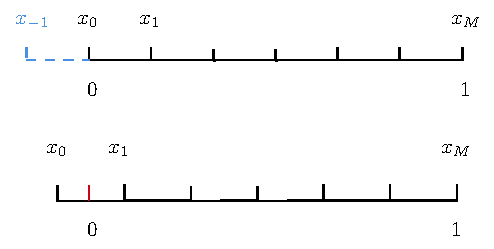
\includegraphics[width=.5\textwidth]{tikz/discrete-grid.pdf}
    \caption{整网格(以及左侧虚拟点)和(左侧)半网格示意图} \label{fig:discrete-grid}
\end{figure}

\section{一维对流方程的边界处理}

对流方程的边界条件设置需要根据风向确定,例如对于入流边界 $x=1$ 和出流边界 $x=0$,
只有入流边界需要提供边界条件 $u(1,t) = \varphi(t)$,对于出流边界不应该提供边界条件,差分格式在处理出流边界时通常有如下办法:
\begin{enumerate}
    \item 对于单边迎风格式,此时无需特殊的边界处理;
    \item 对于 Lax-Wendroff 格式,Lax–Friedrichs 格式等双边离散的格式,需要设计人工出流边界,即更新 $v_0^{n+1}$ 的公式:包括直接利用内部点外插,以及利用特征线求解等。
\end{enumerate}


\section{初边值问题的性质分析}

初值问题与初边值问题的差分格式在分析时的最大区别:
\begin{itemize}
    \item 初值问题:$\Delta x$ 减小时,考虑的空间序列仍是同一个序列空间(无限维空间);
    \item 初边值问题:$\Delta x$ 减小时,考虑的空间序列会发生变化(空间维度逐渐提升的有限维空间)。没有一个合适的空间可以定义差分格式的收敛性,必须考虑一个变化的空间序列以及相应的模序列。
\end{itemize}


考虑有界区域 $[0,1]$,默认考虑均匀剖分并对网格逐渐加密:设第 $k$ 个网格含两侧边界的格点数为 $M_k+1$,
网格尺度 $\Delta x^{(k)} = \frac{1}{M_k}$,满足 $\Delta x^{(k)} \to 0\,(k \to \infty)$。
第 $k$ 个网格的离散点序列为
\[
    0 = x_0^{(k)} < x_1^{(k)} < \cdots < x_{M_k}^{(k)} = 1, \quad x_j^{(k)} = j \Delta x^{(k)}.
\]
对应的数值解和精确解记作
\[
    V^{n,(k)} = \{v_0^{n,(k)},v_1^{n,(k)},\cdots,v_{M_k}^{n,(k)}\}, \quad
    U^{n,(k)} = \{u_0^{n,(k)},u_1^{n,(k)},\cdots,u_{M_k}^{n,(k)}\}
\]
对应的有限维空间 $X^{(k)}$ 具有范数 $\|\cdot\|_k$。

\subsection{相容性}

\begin{definition}[局部截断误差]
    对于偏微分方程 $\mathcal{L} u = g$ 以及对应的差分格式 $L v_j^n = g_j^n$,
    定义在 $(x_j,t^n)$ 处的局部截断误差为
    \[
        \tau_j^n = L u_j^n - g_j^n - (\mathcal{L}u(x_j,t^n) - g(x_j,t^n)) = L u_j^n - g_j^n
    \]
    其中 $u(x,t)$ 是满足偏微分方程的充分光滑函数。在内部和边界计算得到的局部截断误差可能不一样。
\end{definition}

\begin{definition}[逐点相容性]
    称偏微分方程 $\mathcal{L} u = g$ 对应的差分格式 $L v_j^n = g_j^n$ 是(无条件)逐点相容的:如果局部截断误差 $\tau_j^n$ 在
    $\Delta x^{(k)},\Delta t^{(k)}\to 0$ 时满足
    \[
        \tau_j^n \to 0.
    \]
    进一步,称这个格式的局部截断误差阶是 $(p,q)$ :如果存在不可改善的正数 $p,q$,使得下式成立
    \[
        \tau_j^n = \mathcal{O}((\Delta x^{(k)})^p + (\Delta t^{(k)})^q)
    \]
    由于通常对内部和边界采用了不同的近似处理,在内部和边界计算得到的局部截断误差阶可能不一样,差分格式的局部截断误差阶取两者中的最小值。
\end{definition}



\begin{definition}[模相容性]\label{def:ib-norm-consistency}
    对于初边值问题的双层格式
    \[
        V^{n+1,(k)} = Q \, V^{n,(k)} + \Delta t^{(k)}\, G^{n,(k)}
    \]
    将满足偏微分方程的充分光滑函数 $U$ 代入会产生余项 $\Delta t^{(k)}\, T^{n,(k)}$
    \[
        U^{n+1,(k)} = Q \, U^{n,(k)} + \Delta t^{(k)}\, G^{n,(k)} + \Delta t^{(k)}\, T^{n,(k)}
    \]
    称差分格式是(无条件)关于 $\|\cdot\|_k$ 模相容的:
    如果随着 $k \to \infty$,$\Delta t^{(k)} \to 0$,$n \Delta t^{(k)} \to t^*$,有
    \[
        \|T^{n,(k)}\|_{k} \to 0
    \]
    进一步,称这个格式的 $\|\cdot\|_k$ 模相容阶是 $(p,q)$:如果存在不可改善的正数 $p,q$,使得下式成立
    \[
        \|T^{n,(k)}\|_{k} = \mathcal{O}((\Delta x^{(k)})^p + (\Delta t^{(k)})^q)
    \]
\end{definition}

\begin{remark}
    对于初边值问题,整理为向量形式的差分格式是包括内部离散和边界离散的,尤其注意的是,对于边界附近的点值,实际的计算格式是由内部离散和边界离散耦合得到的。
\end{remark}

\begin{remark}
    对于隐格式,通常可以整理为如下形式
    \[
        P V^{n+1,(k)} = Q \, V^{n,(k)} + \Delta t^{(k)}\, G^{n,(k)}
    \]
    此时不需要计算 $P^{-1}$ 来整理为定义~\ref{def:ib-norm-consistency} 中的形式,直接将精确解代入格式两侧
    \[
        P U^{n+1,(k)} = Q \, U^{n,(k)} + \Delta t^{(k)}\, G^{n,(k)} + \Delta t^{(k)}\, T^{n,(k)}
    \]
    模相容性仍然通过 $T^{n,(k)}$ 来体现。
\end{remark}

\begin{remark}
    这里采用了教材 J.W.Thomas《Numerical Partial Differential Equations: Finite Difference Methods》2.3.2 节中的观点:
    逐点相容性只考虑内部差分格式对于偏微分方程的近似,或只考虑边界离散处理对边界条件的近似效果,并不考虑两者的耦合;
    模相容性则是考虑两者在边界附近的耦合得到的实际格式。
    但是这种观点与张强《偏微分方程的有限差分方法》3.4 节并不一致,后者所讨论的局部截断误差是针对两者耦合之后的实际格式进行的分析。
    不过两本教材的相关例子都说明了不合适的边界离散会导致整体出现掉阶现象。
\end{remark}

\subsection{稳定性}

\begin{definition}[模稳定性]
    对于初边值问题的双层格式
    \[
        V^{n+1} = Q \, V^{n}
    \]
    称差分格式是关于 $\|\cdot\|_k$ 模稳定的:
    如果存在常数 $K,\beta > 0$,以及正的 $\Delta x_0,\Delta t_0$,
    使得对于任意 $0 < \Delta x^{(k)} \le \Delta x_0$、$0 < \Delta t^{(k)} \le \Delta t_0$,
    以及 $0 \le t = (n+1)\Delta t^{(k)}$,有
    \[
        \|V^{n+1,(k)}\|_{k} \le K e^{\beta t} \| V^{0,(k)}\|_k
    \]
\end{definition}

根据定义很容易得到模稳定性的充要条件:
\begin{theorem}
    对于初边值问题的双层差分格式
    \[
        V^{n+1} = Q \, V^{n}
    \]
    差分格式是关于 $\|\cdot\|_k$ 模稳定的充要条件是:
    存在常数 $K,\beta > 0$,以及正的 $\Delta x_0,\Delta t_0$,
    使得对于任意 $0 < \Delta x^{(k)} \le \Delta x_0$、$0 < \Delta t^{(k)} \le \Delta t_0$,
    以及 $0 \le t = (n+1)\Delta t^{(k)}$,有
    \[
        \|Q^{n+1}\|_{k} \le K e^{\beta t}
    \]
\end{theorem}

如果特别取 $\|\cdot\|_k$ 为具体的模,可以得到一些与矩阵 $Q$ 相关的稳定性条件。

\begin{theorem}
    对于初边值问题的双层差分格式
    \[
        V^{n+1} = Q \, V^{n}
    \]
    关于 $\|\cdot\|_{2,k}$ 模稳定的必要条件是:
    存在常数 $C \ge 0$,使得
    \[
        \sigma(Q) = \max_i|\lambda_i(Q)| \le 1 + C\,\Delta t
    \]
\end{theorem}

\begin{theorem}
    对于初边值问题的双层差分格式
    \[
        V^{n+1} = Q \, V^{n}
    \]
    关于最大模 $\|\cdot\|_{\infty,k}$ 稳定的一个充分条件是 $\|Q\|_{\infty,k} \le 1$。
\end{theorem}

\subsection{收敛性}


\begin{definition}[模收敛性]
    对于初边值问题的双层差分格式
    \[
        V^{n+1,(k)} = Q \, V^{n,(k)} + \Delta t^{(k)}\, G^{n,(k)}
    \]
    称这个格式是(无条件)关于 $\|\cdot\|_k$ 模收敛的:如果随着 $k \to \infty$,$\Delta t^{(k)} \to 0$,$(n+1) \Delta t^{(k)} \to t^*$,有
    \[
        \|U^{n+1,(k)} - V^{n+1,(k)}\|_{k} \to 0
    \]
    其中 $U$ 是满足偏微分方程的充分光滑函数。
    进一步,称这个格式关于 $\|\cdot\|_k$ 模的收敛阶是 $(p,q)$:如果存在不可改善的正数 $p,q$,使得下式成立
    \[
        \|U^{n+1,(k)} - V^{n+1,(k)}\|_{k} = \mathcal{O}((\Delta x^{(k)})^p + (\Delta t^{(k)})^q)
    \]
\end{definition}


\subsection{Lax定理}


\begin{theorem}[Lax定理]
    对于一个适定的线性偏微分方程初边值问题的双层差分格式
    \[
        V^{n+1,(k)} = Q \, V^{n,(k)} + \Delta t\, G^{n,(k)}
    \]
    若其关于 $\|\cdot\|_k$ 模的相容阶是 $(p,q)$,并且它关于 $\|\cdot\|_k$ 模稳定,那么该格式关于 $\|\cdot\|_k$ 模的收敛阶是 $(p,q)$。
\end{theorem}

\subsection{一些例子}

主要关注一维常系数扩散方程的初边值问题分析。

\subsubsection{Dirichlet边界}

考虑如下扩散方程初边值问题($b > 0$),左右均为Dirichlet边界
\[
    \left\{
    \begin{aligned}
         & u_t = b u_{xx},      &  & x \in (0,1),\, t > 0, \\
         & u(x,0) = u_0(x),     &  & x \in [0,1],          \\
         & u(0,t) = u(1,t) = 0, &  & t \ge 0.
    \end{aligned}
    \right.
\]
在边界直接赋值,得到差分格式(记 $\mu = \frac{ b \Delta t}{\Delta x^2}$)
\begin{equation}
    \left\{
    \begin{aligned}
         & v_j^{n+1} = v_j^n + \mu \delta_x^2 v_j^n, &  & j=1,\dots,M_k-1,\, n=0,1,\dots, \\
         & v_j^0 = u_0(x_j),                         &  & j=0,\dots,M_k,                  \\
         & v_0^{n+1} = v_{M_k}^{n+1} = 0,            &  & n=0,1,\dots.
    \end{aligned}
    \right. \label{eq:ib-1}
\end{equation}


\begin{example}
    当 $0 < \mu \le \frac12$ 时,差分格式~\eqref{eq:ib-1} 关于最大模 $\|\cdot\|_{\infty}$ 稳定 \& 收敛。
\end{example}

\begin{proof}
    直接放缩可以证明最大模稳定性
    \begin{align*}
        v_{j}^{n+1} ={}     &
        v_j^{n} + \mu (v_{j+1}^{n}-2v_j^{n}+v_{j-1}^{n})                        \\
        ={}                 & \mu v_{j+1}^{n} + (1-2\mu)v_j^{n}+\mu v_{j-1}^{n} \\
        |v_{j}^{n+1}| \le{} &
        \mu |v_{j+1}^{n}| + (1-2\mu)|v_j^{n}|+\mu |v_{j-1}^{n}| \le{}  \|V^{n}\|_{\infty}
    \end{align*}
    因此 $\|V^{n+1}\|_{\infty} \le{} \|V^{n}\|_{\infty}$。

    对于数值解 $v_{j}^{n+1}$ 和精确解 $u_{j}^{n+1}$,满足
    \begin{align*}
        v_{j}^{n+1} & = v_j^{n} + \mu \delta_x^2 v_j^{n},                       \\
        u_{j}^{n+1} & = u_j^{n} + \mu \delta_x^2 u_j^{n} + \Delta t \tau_j^{n},
    \end{align*}
    其中局部截断误差为 $\tau_j^{n} = \mathcal{O}(\Delta x^2 + \Delta t)$。
    将两式作差,定义 $z_{j}^{n+1}=u_{j}^{n+1}-v_{j}^{n+1}$
    \begin{align*}
        z_{j}^{n+1} ={}     &
        z_j^{n} + \mu (z_{j+1}^{n}-2z_j^{n}+z_{j-1}^{n}) + \Delta t \tau_j^{n}
        \\
        ={}                 & \mu z_{j+1}^{n} + (1-2\mu)z_j^{n}+\mu z_{j-1}^{n}+ \Delta t \tau_j^{n}
        \\
        |z_{j}^{n+1}| \le{} &
        \mu |z_{j+1}^{n}| + (1-2\mu)|z_j^{n}| + \mu |z_{j-1}^{n}| + \Delta t A (\Delta x^2 + \Delta t)
        \\
        \le{}               & \|Z^{n}\|_{\infty}+ \Delta t A (\Delta x^2 + \Delta t)
    \end{align*}
    遍历所有的 $j$ 使得左侧取到最大值 $\|Z^{n+1}\|_{\infty}$,可得
    \begin{align*}
        \|Z^{n+1}\|_{\infty} \le{} & \|Z^{n}\|_{\infty}+ \Delta t A (\Delta x^2 + \Delta t)
        \\ \le{} & \cdots \le (n+1)\Delta t A (\Delta x^2 + \Delta t) \\
        ={}                        & t^* A (\Delta x^2 + \Delta t) \to 0.
    \end{align*}
    得证最大模收敛性,最大模收敛阶为 $(2,1)$。
\end{proof}


\subsubsection{Neumann、Robin 边界(整网格)}

考虑如下扩散方程初边值问题($b > 0$),左侧为Robin 边界($\sigma \ge 0$),右侧为Dirichlet边界
\[
    \left\{
    \begin{aligned}
         & u_t = b u_{xx},                 &  & x \in (0,1),\, t > 0, \\
         & u(x,0) = u_0(x),                &  & x \in [0,1],          \\
         & - u_x(0,t) + \sigma u(0,t) = 0, &  & t \ge 0,              \\
         & u(1,t) = 0,                     &  & t \ge 0.
    \end{aligned}
    \right.
\]
左侧边界使用单侧差商离散
\[
    -  \frac{v_1^n - v_0^n}{\Delta x} + \sigma v_0^n = 0, \quad \Rightarrow \quad v_0^n = \frac{1}{1 + \sigma \Delta x} v_1^n
\]
得到差分格式(记 $\mu = \frac{b \Delta t}{\Delta x^2}$)
\begin{equation}
    \left\{
    \begin{aligned}
         & v_j^{n+1} = v_j^n + \mu \delta_x^2 v_j^n,            &  & j=1,\dots,M_k-1,\, n=0,1,\dots, \\
         & v_j^0 = u_0(x_j),                                    &  & j=0,\dots,M_k,                  \\
         & v_0^{n+1} = \frac{1}{1 + \sigma \Delta x} v_1^{n+1}, &  & n=0,1,\dots.                    \\
         & v_{M_k}^{n+1} = 0,                                   &  & n=0,1,\dots.
    \end{aligned}
    \right.    \label{eq:ib-2}
\end{equation}

\begin{example}
    当 $0 < \mu \le \frac12$ 时,差分格式~\eqref{eq:ib-2} 在最大模 \& $L^2$ 模意义下是稳定的。
\end{example}

\begin{proof}
    将格式写作 $V^{n+1} = Q\, V^n$ 的形式(不含 $v_0$ 和 $v_{M}$)
    \[
        \begin{bmatrix}
            v_1^{n+1} \\ v_2^{n+1} \\ \vdots \\ v_{M-2}^{n+1} \\ v_{M-1}^{n+1}
        \end{bmatrix}
        =
        \begin{bmatrix}
            1-2\mu + \frac{\mu}{1+\sigma \Delta x} & \mu    &        &        &        \\
            \mu                                    & 1-2\mu & \mu    &        &        \\
                                                   & \ddots & \ddots & \ddots &        \\
                                                   &        & \mu    & 1-2\mu & \mu    \\
                                                   &        &        & \mu    & 1-2\mu \\
        \end{bmatrix}
        \begin{bmatrix}
            v_1^{n} \\ v_2^{n} \\ \vdots \\ v_{M-2}^{n} \\ v_{M-1}^{n}
        \end{bmatrix}
    \]
    稳定性只需要证明无穷范数 $\|Q\|_{\infty} \le 1$
    和谱半径 $\sigma(Q) \le 1$,对于矩阵 $Q$,这两个结论显然成立。
\end{proof}

\begin{example}
    差分格式~\eqref{eq:ib-2} 是逐点相容的。
\end{example}

\begin{proof}
    对于内部离散,将精确解 $u$ 代入可得
    \[
        \tau_j^n = \frac{u_{j}^{n+1}-u_j^n}{\Delta t} - \frac{u_{j+1}^{n}-2u_{j}^{n}+u_{j-1}^{n}}{\Delta x^2}
        = \mathcal{O}(\Delta x^2 + \Delta t)
    \]
    对于边界离散,将精确解 $u$ 代入可得
    \[
        \tau_0^n = - \frac{u_1^n - u_0^n}{\Delta x} + \sigma u_0^n = \mathcal{O}(\Delta x)
    \]
    因此格式是逐点相容的,局部截断误差阶是 $(1,1)$。
\end{proof}

\begin{example}
    差分格式~\eqref{eq:ib-2} 是最大模不相容的。
\end{example}

\begin{proof}
    将精确解 $u$ 代入格式~\eqref{eq:ib-2} 的矩阵形式,产生余项 $\Delta t\, T^n$
    \[
        \begin{bmatrix}
            u_1^{n+1} \\ u_2^{n+1} \\ \vdots \\ u_{M-2}^{n+1} \\ u_{M-1}^{n+1}
        \end{bmatrix}
        =
        \begin{bmatrix}
            1-2\mu + \frac{\mu}{1+\sigma \Delta x} & \mu    &        &        &        \\
            \mu                                    & 1-2\mu & \mu    &        &        \\
                                                   & \ddots & \ddots & \ddots &        \\
                                                   &        & \mu    & 1-2\mu & \mu    \\
                                                   &        &        & \mu    & 1-2\mu \\
        \end{bmatrix}
        \begin{bmatrix}
            u_1^{n} \\ u_2^{n} \\ \vdots \\ u_{M-2}^{n} \\ u_{M-1}^{n}
        \end{bmatrix}
        +
        \Delta t
        \begin{bmatrix}
            T_1^{n} \\ T_2^{n} \\ \vdots \\ T_{M-2}^{n} \\ T_{M-1}^{n}
        \end{bmatrix}
    \]
    易知 $T_j^{n} = \mathcal{O}( \Delta x^2 + \Delta t)$,$j=2,\dots,M-1$,
    只需要关注 $T_1^{n}$
    \begin{align*}
        \Delta t\, T_1^{n} ={} & u_1^{n+1} - \left(1-2\mu + \frac{\mu}{1+\sigma \Delta x}\right) u_1^n - \mu u_2^n \\
        ={}                    & \mu \left(u_0^n - \frac{1}{1+\sigma \Delta x} u_1^n\right)
        + \left[
        u_1^{n+1} - u_1^n - \mu(u_0^n - 2 u_1^n + u_2^n)
        \right]                                                                                                    \\
        ={}                    & \mu \left(u_0^n - \frac{1}{1+\sigma \Delta x} u_1^n\right)
        + \mathcal{O}(\Delta t \Delta x^2 + \Delta t^2)
    \end{align*}
    由边界条件可得
    \begin{gather*}
        -  \frac{u_1^n - u_0^n}{\Delta x} + \sigma u_0^n = -\frac{\Delta x}2 (u_{xx})_1^n + \mathcal{O}(\Delta x^2),\\
        u_0^n - \frac{u_1^n}{1+\sigma \Delta x} = -\frac{\Delta x^2}2 (u_{xx})_1^n + \mathcal{O}(\Delta x^3).
    \end{gather*}
    代入可得
    \[
        \Delta t\, T_1^{n} ={} -\frac{b \Delta t}2 (u_{xx})_1^n + \mathcal{O}(\Delta t^2 \Delta x)+ \mathcal{O}(\Delta t \Delta x^2 + \Delta t^2)
    \]
    因此 $T_1^n = \mathcal{O}(1)$,这直接导致 $\|T^n\|_{\infty} = \mathcal{O}(1)$,因此格式按最大模不相容。
\end{proof}

左侧边界引入虚拟点 $x_{-1}$ 进行双侧离散,得到
\[
    - \frac{v_{1}^{n}-v_{-1}^{n}}{2\Delta x} + \sigma v_0^n = 0, \quad \Rightarrow \quad v_{-1}^{n} = v_0^{n} - 2\sigma \Delta x v_0^n.
\]
得到差分格式(记 $\mu = \frac{b \Delta t}{\Delta x^2}$)
\begin{equation}
    \left\{
    \begin{aligned}
         & v_j^{n+1} = v_j^n + \mu \delta_x^2 v_j^n,                    &  & j=1,\dots,M_k-1,\, n=0,1,\dots, \\
         & v_j^0 = u_0(x_j),                                            &  & j=0,\dots,M_k,                  \\
         & v_0^{n+1} = v_0^n + 2\mu (v_1^n-(1+ \sigma \Delta x) v_0^n), &  & n=0,1,\dots.                    \\
         & v_{M_k}^{n+1} = 0,                                           &  & n=0,1,\dots.
    \end{aligned}
    \right.
    \label{eq:ib-3a}
\end{equation}
还可以将 $v_0^n$ 用空间平均替代,使用如下方式离散
\[
    - \frac{v_{1}^{n}-v_{-1}^{n}}{2\Delta x} + \sigma \frac{v_{-1}^n + v_1^n}2 = 0, \quad \Rightarrow \quad v_{-1}^{n} = \frac{1-\sigma \Delta x}{1+\sigma \Delta x} v_1^n.
\]
得到差分格式(记 $\mu = \frac{b \Delta t}{\Delta x^2}$)
\begin{equation}
    \left\{
    \begin{aligned}
         & v_j^{n+1} = v_j^n + \mu \delta_x^2 v_j^n,                                      &  & j=1,\dots,M_k-1,\, n=0,1,\dots, \\
         & v_j^0 = u_0(x_j),                                                              &  & j=0,\dots,M_k,                  \\
         & v_0^{n+1} = v_0^n + 2\mu \left(\frac{1}{1+\sigma \Delta x}v_1^n- v_0^n\right), &  & n=0,1,\dots.                    \\
         & v_{M_k}^{n+1} = 0,                                                             &  & n=0,1,\dots.
    \end{aligned}
    \right.    \label{eq:ib-3b}
\end{equation}


\begin{example}
    分析差分格式~\eqref{eq:ib-3a} 和~\eqref{eq:ib-3b} 的最大模稳定性。
\end{example}

\begin{proof}
    将格式~\eqref{eq:ib-3a} 和~\eqref{eq:ib-3b} 写作 $V^{n+1} = Q\, V^n$ 的形式(不含 $v_{M}$)
    \[
        \begin{bmatrix}
            v_0^{n+1} \\ v_1^{n+1} \\ \vdots \\ v_{M-2}^{n+1} \\ v_{M-1}^{n+1}
        \end{bmatrix}
        =
        \begin{bmatrix}
            1-2\mu(1+\sigma \Delta x) & 2\mu   &        &        &        \\
            \mu                       & 1-2\mu & \mu    &        &        \\
                                      & \ddots & \ddots & \ddots &        \\
                                      &        & \mu    & 1-2\mu & \mu    \\
                                      &        &        & \mu    & 1-2\mu \\
        \end{bmatrix}
        \begin{bmatrix}
            v_0^{n} \\ v_1^{n} \\ \vdots \\ v_{M-2}^{n} \\ v_{M-1}^{n}
        \end{bmatrix}
    \]
    \[
        \begin{bmatrix}
            v_0^{n+1} \\ v_1^{n+1} \\ \vdots \\ v_{M-2}^{n+1} \\ v_{M-1}^{n+1}
        \end{bmatrix}
        =
        \begin{bmatrix}
            1-2\mu & \frac{2\mu}{1+\sigma \Delta x} &        &        &        \\
            \mu    & 1-2\mu                         & \mu    &        &        \\
                   & \ddots                         & \ddots & \ddots &        \\
                   &                                & \mu    & 1-2\mu & \mu    \\
                   &                                &        & \mu    & 1-2\mu \\
        \end{bmatrix}
        \begin{bmatrix}
            v_0^{n} \\ v_1^{n} \\ \vdots \\ v_{M-2}^{n} \\ v_{M-1}^{n}
        \end{bmatrix}
    \]
    最大模稳定性只需要证明无穷范数 $\|Q\|_{\infty} \le 1$,对于格式~\eqref{eq:ib-3a},这要求
    \[
        2 \mu (1 + \sigma \Delta x) \le 1
    \]
    这表明边界处理导致了稳定性条件需要加强:要求 $\mu < \frac12$ 并且 $\Delta x $ 足够小。
    对于格式~\eqref{eq:ib-3b},最大模稳定性的要求则仍然是通常的 $\mu \le \frac12$。
\end{proof}

\begin{remark}
    这个例子与 Lax-Friedrichs 格式都表明:使用平均值替换可能会改善差分格式的稳定性。
\end{remark}


\begin{example}
    差分格式~\eqref{eq:ib-3a} 和~\eqref{eq:ib-3b} 都是最大模相容的。
\end{example}

\begin{proof}
    只验证格式~\eqref{eq:ib-3b},格式~\eqref{eq:ib-3a} 的分析完全类似。
    将精确解 $u$ 代入格式~\eqref{eq:ib-3b} 的矩阵形式,产生余项 $\Delta t \,T^n$
    \[
        \begin{bmatrix}
            u_0^{n+1} \\ u_1^{n+1} \\ \vdots \\ u_{M-2}^{n+1} \\ u_{M-1}^{n+1}
        \end{bmatrix}
        =
        \begin{bmatrix}
            1-2\mu & \frac{2\mu}{1+\sigma \Delta x} &        &        &        \\
            \mu    & 1-2\mu                         & \mu    &        &        \\
                   & \ddots                         & \ddots & \ddots &        \\
                   &                                & \mu    & 1-2\mu & \mu    \\
                   &                                &        & \mu    & 1-2\mu \\
        \end{bmatrix}
        \begin{bmatrix}
            u_0^{n} \\ u_1^{n} \\ \vdots \\ u_{M-2}^{n} \\ u_{M-1}^{n}
        \end{bmatrix}
        +
        \Delta t
        \begin{bmatrix}
            T_0^{n} \\ T_1^{n} \\ \vdots \\ T_{M-2}^{n} \\ T_{M-1}^{n}
        \end{bmatrix}
    \]
    易知 $T_j^{n} = \mathcal{O}(\Delta x^2 + \Delta t)$,$j=1,\dots,M-1$,只需要关注 $T_0^{n}$
    \begin{align*}
        \Delta t\, T_0^{n} ={} & u_0^{n+1} - (1-2\mu) u_0^n - \frac{2\mu}{1+\sigma \Delta x} u_1^n            \\
        ={}                    & \mu\left(u_{-1}^n - \frac{1-\sigma \Delta x}{1+\sigma \Delta x} u_1^n\right)
        + \left[
        u_0^{n+1} - u_0^n - \mu(u_{-1}^n - 2 u_0^n + u_1^n)
        \right]                                                                                               \\
        ={}                    & \mu\left(u_{-1}^n - \frac{1-\sigma \Delta x}{1+\sigma \Delta x} u_1^n\right)
        + \mathcal{O}(\Delta t \Delta x^2 + \Delta t^2)
    \end{align*}
    由边界条件可得
    \begin{gather*}
        - \frac{u_{1}^{n}-u_{-1}^{n}}{2\Delta x} + \sigma \frac{u_{-1}^n + u_1^n}2 =
        -\frac{\Delta x^2}6 (u_{xxx})_1^n
        + \frac{\sigma \Delta x^2}2 (u_{xx})_1^n
        + \mathcal{O}(\Delta x^4),\\
        u_{-1}^n - \frac{1-\sigma \Delta x}{1+\sigma \Delta x} u_1^n =
        -\frac{\Delta x^3}3 (u_{xxx})_1^n
        +  \sigma \Delta x^3  (u_{xx})_1^n
        + \mathcal{O}(\Delta x^5)
    \end{gather*}
    代入可得
    \[
        \Delta t\, T_0^{n} ={}  b \Delta t \Delta x \left( -\frac13 (u_{xxx})_1^n +\sigma (u_{xx})_1^n \right)
        + \mathcal{O}(\Delta t\Delta x^3) + \mathcal{O}(\Delta t \Delta x^2 + \Delta t^2)
    \]
    因此 $T_0^n = \mathcal{O}(\Delta x + \Delta t)$,$\|T^n\|_{\infty} = \mathcal{O}(\Delta x + \Delta t)$,格式按最大模相容。
\end{proof}

\begin{remark}
    如果 $\sigma = 0$,即边界条件为 $u_x(0,t) = 0$,此时恰可以由方程 $u_t = b u_{xx}$ 推出在边界处 $u_{xxx}(0,t) = 0$,因此 $(u_{xxx})_1^n = \mathcal{O}(\Delta x)$,
    得到 $T_0^n = \mathcal{O}(\Delta x^2 + \Delta t)$,在边界附近不再掉阶。
    下面讨论的几种格式也有类似的现象,即一般边界条件时的最大模相容性会掉阶,但是特别的边界条件 $u_x = 0$ 恰不会掉阶,在下文中不再赘述。
\end{remark}


\subsubsection{Neumann、Robin 边界(半网格)}

考虑如下扩散方程初边值问题($b > 0$),左侧为Robin 边界($\sigma \ge 0$),右侧为Dirichlet边界
\[
    \left\{
    \begin{aligned}
         & u_t = b u_{xx},                 &  & x \in (0,1),\, t > 0, \\
         & u(x,0) = u_0(x),                &  & x \in [0,1],          \\
         & - u_x(0,t) + \sigma u(0,t) = 0, &  & t \ge 0,              \\
         & u(1,t) = 0,                     &  & t \ge 0.
    \end{aligned}
    \right.
\]
和上一节不同的是,这里对左边界采用半网格离散:$x_{0} = \frac{\Delta x}2$,$x_1 = \frac{\Delta x}2$,对右边界仍然使用整网格 $x_{M_k} = 1$。
对左侧边界采用如下方式离散
\[
    - \frac{v_1^n - v_{0}^n}{\Delta x} + \sigma \frac{v_0^n + v_1^n}2 = 0.\quad\Rightarrow\quad v_0^{n} = \frac{1-\frac{\sigma}2 \Delta x}{1 +\frac{\sigma}2 \Delta x}\, v_1^{n}
\]
得到差分格式(记 $\mu = \frac{b \Delta t}{\Delta x^2}$)
\begin{equation}
    \left\{
    \begin{aligned}
         & v_j^{n+1} = v_j^n + \mu \delta_x^2 v_j^n,                                             &  & j=1,\dots,M_k-1,\, n=0,1,\dots, \\
         & v_j^0 = u_0(x_j),                                                                     &  & j=0,\dots,M_k,                  \\
         & v_0^{n+1} = \frac{1-\frac{\sigma}2 \Delta x}{1 +\frac{\sigma}2 \Delta x}\, v_1^{n+1}, &  & n=0,1,\dots.                    \\
         & v_{M_k}^{n+1} = 0,                                                                    &  & n=0,1,\dots.
    \end{aligned}
    \right.    \label{eq:ib-5}
\end{equation}

\begin{example}
    分析差分格式~\eqref{eq:ib-5} 的最大模稳定性。
\end{example}

\begin{proof}
    将格式写作 $V^{n+1} = Q\, V^n$ 的形式(不含 $v_0$ 和 $v_{M}$)
    \[
        \begin{bmatrix}
            v_1^{n+1} \\ v_2^{n+1} \\ \vdots \\ v_{M-2}^{n+1} \\ v_{M-1}^{n+1}
        \end{bmatrix}
        =
        \begin{bmatrix}
            1-2\mu + \mu\frac{1-\frac{\sigma}2 \Delta x}{1 + \frac{\sigma}2 \Delta x} & \mu    &        &        &        \\
            \mu                                                                       & 1-2\mu & \mu    &        &        \\
                                                                                      & \ddots & \ddots & \ddots &        \\
                                                                                      &        & \mu    & 1-2\mu & \mu    \\
                                                                                      &        &        & \mu    & 1-2\mu \\
        \end{bmatrix}
        \begin{bmatrix}
            v_1^{n} \\ v_2^{n} \\ \vdots \\ v_{M-2}^{n} \\ v_{M-1}^{n}
        \end{bmatrix}
    \]
    最大模稳定性只需要证明无穷范数 $\|Q\|_{\infty} \le 1$,显然只需要 $\mu \le \frac12$ 即可保证。
\end{proof}

\begin{example}
    差分格式~\eqref{eq:ib-5} 是最大模相容的。
\end{example}

\begin{proof}
    将精确解 $u$ 代入格式~\eqref{eq:ib-5} 的矩阵形式,产生余项 $\Delta t \,T^n$
    \[
        \begin{bmatrix}
            u_1^{n+1} \\ u_2^{n+1} \\ \vdots \\ u_{M-2}^{n+1} \\ u_{M-1}^{n+1}
        \end{bmatrix}
        =
        \begin{bmatrix}
            1-2\mu + \mu\frac{1-\frac{\sigma}2 \Delta x}{1 + \frac{\sigma}2 \Delta x} & \mu    &        &        &        \\
            \mu                                                                       & 1-2\mu & \mu    &        &        \\
                                                                                      & \ddots & \ddots & \ddots &        \\
                                                                                      &        & \mu    & 1-2\mu & \mu    \\
                                                                                      &        &        & \mu    & 1-2\mu \\
        \end{bmatrix}
        \begin{bmatrix}
            u_1^{n} \\ u_2^{n} \\ \vdots \\ u_{M-2}^{n} \\ u_{M-1}^{n}
        \end{bmatrix}
        +
        \Delta t
        \begin{bmatrix}
            T_1^{n} \\ T_2^{n} \\ \vdots \\ T_{M-2}^{n} \\ T_{M-1}^{n}
        \end{bmatrix}
    \]
    易知 $T_j^{n} = \mathcal{O}(\Delta x^2 + \Delta t)$,$j=2,\dots,M-1$,只需要关注 $T_1^{n}$
    \begin{align*}
        \Delta t\, T_1^{n} ={} & u_1^{n+1} - \left(1-2\mu + \mu \frac{1-\frac{\sigma}2 \Delta x}{1 + \frac{\sigma}2 \Delta x}\right) u_2^n
        - \mu u_1^n                                                                                                                        \\
        ={}                    & \mu\left( u_{0}^n -  \frac{1-\frac{\sigma}2 \Delta x}{1 + \frac{\sigma}2 \Delta x} u_1^n \right)
        + \left[
        u_1^{n+1} - u_1^n - \mu(u_{0}^n - 2 u_1^n + u_2^n)
        \right]                                                                                                                            \\
        ={}                    & \mu\left( u_{0}^n -  \frac{1-\frac{\sigma}2 \Delta x}{1 + \frac{\sigma}2 \Delta x} u_1^n \right)
        + \mathcal{O}( \Delta t \Delta x^2 + \Delta t^2)
    \end{align*}
    由边界条件可得
    \begin{gather*}
        - \frac{u_1^n - u_{0}^n}{\Delta x} + \sigma \frac{u_0^n + u_1^n}2 = -\frac{\Delta x^2}{24} (u_{xxx})_1^n + \frac{\sigma \Delta x^2}8 (u_{xx})_1^n + \mathcal{O}(\Delta x^4) \\
        u_{0}^n -  \frac{1-\frac{\sigma}2 \Delta x}{1 + \frac{\sigma}2 \Delta x} u_1^n = -\frac{\Delta x^3}{24} (u_{xxx})_1^n + \frac{\sigma \Delta x^3}8 (u_{xx})_1^n + \mathcal{O}(\Delta x^5)
    \end{gather*}
    代入可得
    \[
        \Delta t\, T_1^{n} ={} b \Delta t \Delta x \left( -\frac1{24} (u_{xxx})_1^n + \frac{\sigma}8 (u_{xx})_1^n \right)
        + \mathcal{O}(\Delta t\Delta x^3) + \mathcal{O}( \Delta t \Delta x^2 + \Delta t^2)
    \]
    因此 $T_1^n = \mathcal{O}(\Delta x + \Delta t)$,$\|T^n\|_{\infty} = \mathcal{O}(\Delta x + \Delta t)$,格式按最大模相容。
\end{proof}


考虑对左侧边界使用半网格,对应如下方式离散
\[
    - \frac{v_1^n - v_{0}^n}{\Delta x} + \sigma \frac{v_0^n + v_1^n}2 = 0.\quad\Rightarrow\quad v_0^{n} = \frac{1-\frac{\sigma}2 \Delta x}{1 +\frac{\sigma}2 \Delta x}\, v_1^{n}
\]
在时间上使用 Crank–Nicolson 格式,得到的差分格式矩阵形式如下(不含 $v_0$ 和 $v_{M}$)(记 $\mu = \frac{b \Delta t}{\Delta x^2}$)
{\small\[
    \begin{bmatrix}
        1+\mu - \frac{\mu}{2}\left(\frac{1-\frac{\sigma}2 \Delta x}{1 +\frac{\sigma}2 \Delta x}\right) & -\frac{\mu}2 &              &              \\
        -\frac{\mu}2                                                                                   & 1+\mu        & \ddots       &              \\
                                                                                                       & \ddots       & \ddots       & -\frac{\mu}2 \\
                                                                                                       &              & -\frac{\mu}2 & 1+\mu        \\
    \end{bmatrix}
    \begin{bmatrix}
        v_1^{n+1} \\ v_2^{n+1} \\ \vdots  \\ v_{M-1}^{n+1}
    \end{bmatrix}
    =
    \begin{bmatrix}
        1 -\mu + \frac{\mu}{2}\left(\frac{1-\frac{\sigma}2 \Delta x}{1 +\frac{\sigma}2 \Delta x}\right) & \frac{\mu}2 &             &             \\
        \frac{\mu}2                                                                                     & 1-\mu       & \ddots      &             \\
                                                                                                        & \ddots      & \ddots      & \frac{\mu}2 \\
                                                                                                        &             & \frac{\mu}2 & 1-\mu       \\
    \end{bmatrix}
    \begin{bmatrix}
        v_1^{n} \\ v_2^{n} \\ \vdots  \\ v_{M-1}^{n}
    \end{bmatrix}
\]}

\begin{example}
    分析左侧边界使用半网格离散的 Crank–Nicolson 格式的最大模相容性。
\end{example}

\begin{proof}
    将精确解 $u$ 代入格式~\eqref{eq:ib-5} 的矩阵形式,产生余项 $\Delta t \,T^{n+\frac12}$。
    易知 $T_j^{n+\frac12} = \mathcal{O}(\Delta x^2 + \Delta t^2)$,$j=2,\dots,M-1$,只需要关注 $T_1^{n+\frac12}$。
    \begin{align*}
        \Delta t\, T_1^{n+\frac12} ={} &
        \left[ 1 + \mu - \frac{\mu}{2}\left(\frac{1-\frac{\sigma}2 \Delta x}{1 +\frac{\sigma}2 \Delta x}\right) \right] u_1^{n+1} - \frac{\mu}2 u_2^{n+1}
        - \left\{\left[ 1 - \mu + \frac{\mu}{2}\left(\frac{1-\frac{\sigma}2 \Delta x}{1 +\frac{\sigma}2 \Delta x}\right) \right] u_1^{n} + \frac{\mu}2 u_2^{n}\right\}              \\
        ={}                            & \left[
        (1+\mu) u_1^{n+1} - \frac{\mu}2 u_0^{n+1} - \frac{\mu}2 u_2^{n+1}
        \right]
        -
        \left[
        (1-\mu) u_1^{n} + \frac{\mu}2 u_0^{n} + \frac{\mu}2 u_2^{n}
        \right]                                                                                                                                                                     \\
                                       & + \frac{\mu}2 \left( u_0^{n+1} - \frac{1-\frac{\sigma}2 \Delta x}{1 +\frac{\sigma}2 \Delta x}u_1^{n+1} \right)
        + \frac{\mu}2 \left( u_0^{n} - \frac{1-\frac{\sigma}2 \Delta x}{1 +\frac{\sigma}2 \Delta x}u_1^{n} \right)                                                                  \\
        ={}                            & \frac{\mu}2 \left[ -\frac{\Delta x^3}{24} (u_{xxx})_1^{n+1} + \frac{\sigma \Delta x^3}8 (u_{xx})_1^{n+1} + \mathcal{O}(\Delta x^5) \right]
        \\ &+ \frac{\mu}2 \left[ -\frac{\Delta x^3}{24} (u_{xxx})_1^n + \frac{\sigma \Delta x^3}8 (u_{xx})_1^n + \mathcal{O}(\Delta x^5) \right]
        + \mathcal{O}(\Delta t \Delta x^2 + \Delta t^3)                                                                                                                             \\
        ={}                            & \mu \left\{
        -\frac{\Delta x^3}{24} (u_{xxx})_1^{n+\frac12} + \frac{\sigma \Delta x^3}8 (u_{xx})_1^{n+\frac12} + \mathcal{O}(\Delta x^5)
        \right\} + \mathcal{O}(\Delta t \Delta x^2 + \Delta t^3)
    \end{align*}
    因此
    \[
        \Delta t\, T_1^{n+\frac12} ={} b \Delta t \Delta x \left( -\frac1{24} (u_{xxx})_1^{n+\frac12} + \frac{\sigma}8 (u_{xx})_1^n \right)
        + \mathcal{O}(\Delta t\Delta x^3) + \mathcal{O}( \Delta t \Delta x^2 + \Delta t^3)
    \]
    因此 $T_1^{n+\frac12} = \mathcal{O}(\Delta x + \Delta t^2)$,$\|T^{n+\frac12}\|_{\infty} = \mathcal{O}(\Delta x + \Delta t^2)$,格式按最大模相容。
\end{proof}

\begin{remark}
    虽然这里对 Crank–Nicolson 格式的相容性分析仍然也会掉阶,但是实际上无论采用何种边界离散,Crank–Nicolson 格式都可以达到整体二阶的最大模收敛性,
    此时 Lax 等价定理无法给予理论支持,还需要借助椭圆型差分格式的强最大值原理,具体参考张强《偏微分方程的有限差分方法》的 3.4 节和 10.2 节。
\end{remark}


\subsection{能量稳定性}

\subsubsection{对流方程}

考虑对流方程初边值问题
\[
    \left\{
    \begin{aligned}
         & u_t = u_{x},   &  & x \in (0,1),\, t > 0, \\
         & u(x,0) = f(x), &  & x \in [0,1],          \\
         & u(1,t) = g(t), &  & t \ge 0.
    \end{aligned}
    \right.
\]
易知 PDE 具有如下性质
\[
    \frac{d}{dt}\|u\|^2 = (u,u_t) + (u_t,u) = (u,u_x) + (u_x,u)
    = |u|^2 \big|_0^1 = |g(t)|^2 - |u(0,t)|^2
\]

\begin{example}
    分析如下半离散格式的能量稳定性
    \[
        \left\{
        \begin{aligned}
             & \frac{d v_j}{d t} = D_+ v_j, &  & j=0,\dots,M-1, \\
             & v_j(0) = f_j,                &  & j=0,\dots,M,   \\
             & v_M(t) = g(t),               &  & t \ge 0.
        \end{aligned}
        \right.
    \]
\end{example}

\begin{solution*}
    \begin{align*}
        \frac{d}{dt} \|v\|_{0,N-1}^2
        ={}                & \left( v,\frac{d v}{d t} \right)_{0,N-1} + \left( \frac{d v}{d t}, v\right)_{0,N-1} \\
        ={}                & \left( v,D_+ v \right)_{0,N-1} + \left( D_+ v, v\right)_{0,N-1}                     \\
        \overset{(*)}{=}{} & - \Delta x \|D_+ v\|_{0,N-1}^2 + |v_N(t)|^2 - |v_0(t)|^2 \le{}  |g(t)|^2
    \end{align*}
    其中的 $(*)$ 利用了如下恒等式,相当于离散版本的“分部积分”
    \[
        (u,D_+ v)_{r,s} + (D_+ u, v)_{r,s} = -\Delta x (D_+ u, D_+ v)_{r,s} + \overline{u}_j v_j \big|_r^{s+1}. \qedhere
    \]
\end{solution*}

\begin{example}
    分析如下FTFS格式的能量稳定性
    \[
        \left\{
        \begin{aligned}
             & v_j^{n+1} = v_j^n + \Delta t D_+ v_j, &  & j=0,\dots,M-1, \\
             & v_j^0 = f_j,                          &  & j=0,\dots,M,   \\
             & v_M^n = g^n,                          &  & n=0,1,\dots.
        \end{aligned}
        \right.
    \]
\end{example}

\begin{solution*}
    \begin{align*}
        \| v^{n+1}\|_{0,N-1}^2
        ={} & \|(I + \Delta t D_+) v^n\|_{0,N-1}^2                    \\
        ={} & \| v^n \|_{0,N-1}^2 + \Delta t^2 \| D_+ v^n\|_{0,N-1}^2
        + \Delta t \left[
            \left( v^n, D_+ v^n \right)_{0,N-1} + \left( D_+ v^n, v^n \right)_{0,N-1}
            \right]
        \\
        ={} & \| v^n \|_{0,N-1}^2 + \Delta t^2 \| D_+ v^n\|_{0,N-1}^2
        + \Delta t \left(
        - \Delta x \| D_+ v^n\|_{0,N-1}^2 + |v^n_N|^2 - |v^n_0|^2
        \right)
    \end{align*}
    当 $\Delta t \le \Delta x$ 时,有
    \[
        \| v^{n+1}\|_{0,N-1}^2 \le \| v^n \|_{0,N-1}^2  + \Delta t |v^n_N|^2
        \le \cdots \le \| v^0 \|_{0,N-1}^2  + \Delta t \sum_{\ell=0}^{n} |g^\ell|^2. \qedhere
    \]
\end{solution*}

\begin{remark}
    这里的记号 $(u,v)_{r,s}$ 表示部分求和的离散内积,$\|u\|_{r,s}$ 表示对应的范数。
    \[
        (u,v)_{r,s} = \sum_{i=r}^{s} \bar{u}_i v_i\, \Delta x.
        \quad \|u\|_{r,s} = \sqrt{(u,v)_{r,s}}.
    \]
\end{remark}

\subsubsection{扩散方程(Dirichlet边界)}

考虑扩散方程初边值问题(Dirichlet边界)
\[
    \left\{
    \begin{aligned}
         & u_t = u_{xx},        &  & x \in (0,1),\, t > 0, \\
         & u(x,0) = f(x),       &  & x \in [0,1],          \\
         & u(0,t) = u(1,t) = 0, &  & t \ge 0.
    \end{aligned}
    \right.
\]
易知 PDE 具有如下性质
\[
    \frac{d}{dt}\|u\|^2 = (u,u_t) + (u_t,u) = (u,u_{xx}) + (u_{xx},u)
    = -2 \|u_x\|^2 + (\bar{u} u_x + \bar{u}_x u) \big|_0^1 = -2 \|u_x\|^2 \le 0
\]

\begin{example}
    假定只考虑实值函数,分析如下半离散格式的能量稳定性
    \[
        \left\{
        \begin{aligned}
             & \frac{d v_j}{d t} = D_+ D_- v_j, &  & j=0,\dots,M-1, \\
             & v_j(0) = f_j,                    &  & j=0,\dots,M,   \\
             & v_0(t) = v_M(t) = 0,             &  & t \ge 0.
        \end{aligned}
        \right.
    \]
\end{example}

\begin{solution*}
    \begin{align*}
        \frac12 \frac{d}{dt} \|v\|_{1,N-1}^2
        ={}                & \left( v,D_+ D_- v \right)_{1,N-1}                                      \\
        \overset{(*)}{=}{} & - \| D_- v\|_{2,N}^2 + v_j D_- v_j \big|_1^N                            \\
        ={}                & - \| D_- v\|_{1,N}^2 + \Delta x (D_- v_1)^2 + v_N D_- v_N - v_1 D_- v_1 \\
        ={}                & - \| D_- v\|_{1,N}^2 \le 0
    \end{align*}
    其中的 $(*)$ 利用了如下恒等式
    \[
        (v,D_+ w)_{r,s} + (D_- v, w)_{r+1,s+1} = \overline{v}_j w_j \big|_r^{s+1}.
    \]
    取 $v = D_- v$ 代入可得
    \[
        (v, D_+ D_- v)_{r,s} + \|D_- v\|^2_{r+1,s+1} = \overline{v}_j D_- v_j \big|_r^{s+1}. \qedhere
    \]
\end{solution*}

\begin{lemma}\label{lemma:ib-1}
    \[
        \| D_+ y \|_{1,N-1}^2 \le \frac{4}{\Delta x^2} \| y \|_{1,N}^2
    \]
\end{lemma}

\begin{proof}
    \[
        \| D_+ y \|_{1,N-1}^2
        =  \frac{1}{\Delta x^2} \sum_{j=1}^{N-1} |y_{j+1} - y_j|^2\, \Delta x
        \le \frac{2}{\Delta x^2} \sum_{j=1}^{N-1}(|y_{j+1}|^2 + |y_j|^2)\, \Delta x
        \le \frac{4}{\Delta x^2} \| y \|_{1,N}^2 \qedhere
    \]
\end{proof}

\begin{example}
    假定只考虑实值函数,分析如下FTCS格式的能量稳定性
    \[
        \left\{
        \begin{aligned}
             & v_j^{n+1} = v_j^n + \Delta t D_+D_- v_j, &  & j=0,\dots,M-1, \\
             & v_j^0 = f_j,                             &  & j=0,\dots,M,   \\
             & v_0^n = v_M^n = 0.                       &  & n=0,1,\dots.
        \end{aligned}
        \right.
    \]
\end{example}

\begin{solution*}
    \begin{align*}
        \| v^{n+1} \|_{1,N-1}^2
        ={} & \|(I + \Delta t D_+D_-) v^n\|_{1,N-1}^2                     \\
        ={} & \| v^n \|_{1,N-1}^2 + \Delta t^2 \| D_+ D_- v^n\|_{1,N-1}^2
        + 2 \Delta t \left( v^n, D_+ D_- v^n \right)_{1,N-1}
        \\
        ={} & \| v^n \|_{1,N-1}^2 + \Delta t^2 \| D_+ D_- v^n\|_{1,N-1}^2
        - 2 \Delta t \| D_- v^n\|_{1,N}^2
    \end{align*}
    根据引理~\ref{lemma:ib-1} 有如下不等式成立
    \[
        \| D_+ D_- v^n\|_{1,N-1}^2 \le \frac{4}{\Delta x^2} \| D_- v^n \|_{1,N}^2
    \]
    代入可得
    \[
        \| v^{n+1} \|_{1,N-1}^2 \le \| v^{n} \|_{1,N-1}^2
        - 2\Delta t \left( 1 - \frac{2\Delta t}{\Delta x^2} \right) \| D_- v^n \|_{1,N}^2
    \]
    因此在 $\Delta t \le \frac12 \Delta x^2$ 时
    \[
        \| v^{n+1} \|_{1,N-1}^2 \le \| v^{n} \|_{1,N-1}^2 \qedhere
    \]
\end{solution*}

\subsubsection{扩散方程(Rubin边界)(半网格)}

\begin{lemma}\label{lemma:ib-2}
    对于 $f \in C^1([0,1])$
    \[
        \|f\|_{\infty}^2 \le \varepsilon \|f_x\|^2 + (1 + \frac{1}{\varepsilon}) \|f\|^2,\quad (\forall\,\varepsilon > 0)
    \]
\end{lemma}

\begin{proof}
    记 $x_1$ 和 $x_2$ 为对应的最值点
    \[
        |f(x_1)| = \min_x |f(x)|,\quad |f(x_2)| = \max_y |f(y)| = \|f\|_{\infty}
    \]
    不妨设 $x_1 < x_2$,则有
    \[
        \int_{x_1}^{x_2} \bar{f} f_x\,dx = |f(x_2)|^2 - |f(x_1)|^2 - \int_{x_1}^{x_2} \bar{f}_x f\,dx
    \]
    因此
    \begin{align*}
        \|f\|_{\infty}^2 - \|f\|^2 \le{}
        \|f\|_{\infty}^2 - |f(x_1)|^2 \le{} & 2 \int_{x_1}^{x_2} |f| |f_x|\,dx
        \le{} 2 \int_0^1 |f| |f_x|\,dx                                         \\
        \le{}                               & 2 \|f_x\|\, \|f\|
        \le \varepsilon \| f_x \|^2 + \frac{1}{\varepsilon} \|f\|^2.
    \end{align*}
    命题得证。
\end{proof}


\begin{lemma}\label{lemma:ib-3}
    \[
        \max_{0 \le j \le N} |f_j|^2 \le \varepsilon \|D_- f\|_{1,N}^2
        + (1 + \frac{1}{\varepsilon}) \|f\|_{0,N}^2,\quad (\forall\,\varepsilon > 0)
    \]
\end{lemma}

\begin{proof}
    记 $\alpha$ 和 $\beta$ 为最值点对应的下标
    \[
        |f_\alpha| = \min_{0 \le j \le N} |f_j|, \quad
        |f_\beta| = \max_{0 \le j \le N} |f_j| = \|f\|_{\infty}
    \]
    不妨设 $\alpha \le \beta$,则有
    \[
        (f,\,D_+ f)_{\alpha,\beta-1} = -(D_-f,\,f)_{\alpha+1,\beta} + |f_\beta|^2 - |f_\alpha|^2
    \]
    因此
    \begin{align*}
        \max_{0 \le j \le N} |f_j|^2 \le{} & \min_{0 \le j \le N} |f_j|^2
        + \|f\|_{\alpha,\beta} \Big( \| D_+ f \|_{\alpha,\beta-1} + \| D_- f \|_{\alpha+1,\beta} \Big)                   \\
        \le{}                              & \|f\|_{0,N}^2 + 2 \|f\|_{0,N} \| D_- f \|_{1,N}                             \\
        \le{}                              & \varepsilon \| D_- f \|_{1,N}^2 + (1 + \frac{1}{\varepsilon}) \|f\|_{0,N}^2
    \end{align*}
    命题得证。
\end{proof}

考虑抛物方程初边值问题(Rubin边界)
\[
    \left\{
    \begin{aligned}
         & u_t = u_{xx},              &  & x \in (0,1),\, t > 0, \\
         & u(x,0) = f(x),             &  & x \in [0,1],          \\
         & u_x(0,t) + r_0 u(0,t) = 0, &  & t \ge 0,              \\
         & u_x(1,t) + r_1 u(1,t) = 0, &  & t \ge 0.
    \end{aligned}
    \right.
\]
易知 PDE 具有如下性质
\begin{align*}
    \frac{d}{dt}\|u\|^2
    ={}                  & (u,u_t) + (u_t,u) = (u,u_{xx}) + (u_{xx},u)
    \\
    ={}                  & -2 \|u_x\|^2 + (\bar{u} u_x + \bar{u}_x u) \big|_0^1
    \\
    \le{}                & -2 \|u_x\|^2 + 2(|r_0|+|r_1|) \|u\|_{\infty}^2,\quad (\varepsilon := \frac{1}{2(|r_0|+|r_1|)})
    \\
    \overset{(*)}{\le}{} & - 2 \|u_x\|^2 + \|u_x\|^2 + \frac{1}{\varepsilon} (1 + \frac{1}{\varepsilon}) \|u\|^2
    \\
    ={}                  & -  \|u_x\|^2 + 2(|r_0|+|r_1|)(2(|r_0|+|r_1|)+1)\|u\|^2
\end{align*}
其中 $(*)$ 利用了引理~\ref{lemma:ib-2}。

对于空间离散采用半网格:$x_0 = -\Delta x/2$,$x_1 = \Delta x/2$,
$x_{N-1} = 1-\Delta x/2$,$x_N = 1+\Delta x/2$。


\begin{example}
    假定只考虑实值函数,分析如下半离散格式的能量稳定性
    \[
        \left\{
        \begin{aligned}
             & \frac{d v_j}{d t} = D_+ D_- v_j,                    &  & j=0,\dots,M-1, \\
             & v_j(0) = f_j,                                       &  & j=0,\dots,M,   \\
             & D_+ v_0(t) + \frac12 r_0 (v_0(t) + v_1(t)) = 0,     &  & t \ge 0,       \\
             & D_- v_N(t) + \frac12 r_1 (v_{N-1}(t) + v_N(t)) = 0, &  & t \ge 0.
        \end{aligned}
        \right.
    \]
\end{example}

\begin{solution*}
    \begin{align*}
        \frac12 \frac{d}{dt} \|v\|_{1,N-1}^2
        ={} & \left( v,D_+ D_- v \right)_{1,N-1}                                             \\
        ={} & - \| D_- v\|_{2,N}^2 + v_j D_- v_j \big|_1^N                                   \\
        ={} & - \| D_- v\|_{2,N}^2 - \frac12 r_1 v_N(v_{N-1}+v_N) + \frac12 r_0 v_1(v_0+v_1)
    \end{align*}
    注意到当 $\Delta x$ 足够小时,有
    \[
        |v_0| \le \text{constant}\, |v_1|,\quad
        |v_N| \le \text{constant}\, |v_{N-1}|.
    \]
    利用引理~\ref{lemma:ib-3} 可得
    \begin{align*}
        v_0 v_1 \le{}     & \text{constant}\, |v_1|^2 \le \varepsilon \|D_-v\|_{2,N}^2 + C(\varepsilon) \|v\|_{1,N}^2,     \\
        v_{N-1} v_N \le{} & \text{constant}\, |v_{N-1}|^2 \le \varepsilon \|D_-v\|_{2,N}^2 + C(\varepsilon) \|v\|_{1,N}^2.
    \end{align*}
    注意到 $\|v\|_{1,N}^2 \le \text{constant}\, \|v\|_{1,N-1}^2$,因此可以取足够小的 $\varepsilon$,使得
    \[
        \frac12 \frac{d}{dt} \|v\|_{1,N-1}^2 \le \text{constant}\, \|v\|_{1,N-1}^2 \qedhere
    \]
\end{solution*}


\section{二维扩散方程的边界处理}

关注二维常系数扩散方程的边界处理,只考虑直边界的情形,例如计算区域为 $[0,1]^2$。

\subsection*{FTCS的边界处理}

与一维的边界处理类似,例如
\begin{enumerate}
    \item Dirichlet 边界条件:直接赋值即可
    \item Nuemann 边界条件:
          \begin{enumerate}
              \item 一阶近似,采用单侧差商来近似导数
              \item 二阶近似,引入虚拟点,或考虑半网格
          \end{enumerate}
\end{enumerate}

\subsection*{过渡层的边界处理}

ADI方法等引入了中间过渡层,过渡层的计算需要特殊的边界处理,考虑竖直边界 $x=0$ 或 $x=1$,边界条件为 $u=g(t)$。

\begin{enumerate}
    \item 对于ADI方法的PR格式:如果用 $t^{n+\frac12}$ 的边界条件赋值会掉阶,中间层只是算子分裂计算所产生的,
          并不是真正对应 $t^{n+\frac12}$ 时间层。可以利用格式相加得到更合适的边界条件
          \begin{align*}
              2 v_{i,j}^{n+\frac12} =   \left(1+\frac12 b \mu_y \delta_y^2\right) v_{j,k}^{n}
              + \left(1-\frac12 b \mu_y \delta_y^2\right) v_{j,k}^{n+1}
              \\
              =   \left(1+\frac12 b \mu_y \delta_y^2\right) g_{j,k}^{n}
              + \left(1-\frac12 b \mu_y \delta_y^2\right) g_{j,k}^{n+1}
          \end{align*}
    \item 对于D'Yakonov格式:如果用 $t^{n+\frac12}$ 的边界条件赋值会掉阶,可以利用格式得到
          \begin{align*}
              v_{j,k}^{*}   =    \left(1-\frac12 b \mu_y \delta_y^2 \right) v_{j,k}^{n+1}
              =  \left(1-\frac12 b \mu_y \delta_y^2 \right) g_{j,k}^{n+1}
          \end{align*}
\end{enumerate}


\chapter{一维双曲守恒律方程理论}

\section{预备知识}

物理上有很多的守恒性质,例如能量守恒,质量守恒和动量守恒,这些守恒性质在一定的假设下都可以在数学上对应为如下形式的偏微分方程
\begin{equation}
    \bm{u}_t + \nabla \cdot \bm{F}(\bm{u}) = 0
    \label{eq:cv-laws}
\end{equation}
其中 $x \in \mathbb{R}^d$,满足守恒性质的未知函数 $\bm{u}: \mathbb{R}^d \times \mathbb{R}^+ \to \mathbb{R}^n$,
以及已知的流通量函数 $\bm{F}:\mathbb{R}^m \to \mathbb{R}^n$。

之所以称为守恒律方程,是因为在一个有限的时空区域 $\Omega \times [t^0,t^1] \subset \mathbb{R}^d \times  \mathbb{R}^+$ 对方程~\eqref{eq:cv-laws} 积分可以得到
\[
    0 = \int_{t^0}^{t^1} \int_{\Omega} \left(\bm{u}_t + \nabla \cdot \bm{F}(\bm{u})\right) \,dx\,dt
    = \int_{\Omega} \bm{u}(x,t^1)\,dx - \int_{\Omega} \bm{u}(x,t^0)\,dx
    + \int_{t^0}^{t^1} \int_{\partial \Omega} \bm{n} \cdot \bm{F}(\bm{u}) \,ds\,dt
\]
其中 $\bm{n}$ 是边界处的单位外法向量,最终得到的结果就体现了守恒性质:
\[
    \int_{\Omega} \bm{u}(x,t^1)\,dx - \int_{\Omega} \bm{u}(x,t^0)\,dx
    = - \int_{t^0}^{t^1}\int_{\partial \Omega} \bm{n} \cdot \bm{F}(\bm{u}) \,ds\,dt
\]
$\int_{\Omega} \bm{u}\,dx$ 的变化量仅仅与边界处的交换 $\bm{n} \cdot \bm{F}(\bm{u})$ 有关,
如果 $\bm{n} \cdot \bm{F}(\bm{u})$ 在 $\partial \Omega$ 始终为0,那么就有
\[
    \int_{\Omega} \bm{u}(x,t)\,dx = \text{constant},\,\forall\, t
\]

我们只考虑一维标量情形下的双曲守恒律方程
\begin{equation}
    u_t + f(u)_x = 0,\quad (x,t) \in \mathbb{R} \times  \mathbb{R}^+
    \label{eq:cv-law-scalar}
\end{equation}
考虑纯初值问题或者具有周期边界条件的初边值问题,其中未知函数 $u: \mathbb{R} \times  \mathbb{R}^+ \to \mathbb{R}$,
以及已知的(连续可微的)流通量函数 $f:\mathbb{R} \to \mathbb{R}$。

\begin{example}
    \noindent
    \begin{itemize}
        \item 取 $f(u) = a u$,其中 $a \in \mathbb{R}$ 为常数,就可以得到最简单的常系数线性对流方程
              \[
                  u_t + a u_x = 0
              \]
        \item 取 $f(u) = \frac12 u^2$,就可以得到最简单的非线性守恒律方程——Burgers 方程
              \[
                  u_t + \left(\frac{u^2}2\right)_x = 0
              \]
    \end{itemize}
\end{example}

对于双曲守恒律方程,如果 $f(u)$ 具有足够光滑性,不妨记 $f'(u) = a(u)$,得到两种形式
\begin{enumerate}
    \item 守恒形式 $u_t + f(u)_x = 0$
    \item 非守恒形式 $u_t + a(u) u_x = 0$
\end{enumerate}
从这两种形式出发设计的差分格式并不等价,具有不同的性质和求解效果。

对于双曲守恒律方程,有一类特殊的问题称为 Riemann 问题:
\[
    \left\{
    \begin{aligned}
        u_t + f(u)_x & = 0,\quad (x,t) \in \mathbb{R} \times  \mathbb{R}^+ \\
        u(x,0)       & =
        \begin{cases}
            u_L & x < 0 \\
            u_R & x > 0
        \end{cases}
    \end{aligned}
    \right.
\]
即 $u(x,t)$ 在 $x = 0$ 的左右两侧分别有不同的常数初值 $u_L \neq u_R$。
对于 Riemann 问题,$f(u)$ 的性质以及 $u_L$ 和 $u_R$ 的取值不同会对解的形态产生显著影响。
在下文中对 Riemann 问题的分类讨论中,我们通常会忽略 $u_L = u_R$ 的平凡情况。

\section{特征线}

双曲型方程具有特征线的性质,例如
\begin{itemize}
    \item \textbf{常系数线性对流方程:} $u_t + a u_x = 0$,从 $x=x_0$ 发出的特征线 $x=x(t)$ 满足如下方程
          \[
              \left\{
              \begin{aligned}
                  \frac{d x(t)}{d t} & = a,   \\
                  x(0)               & = x_0.
              \end{aligned}
              \right. \quad \Rightarrow \quad x = x_0 + a t
          \]
          特征线为 $t\!-\!x$ 平面的一族平行直线,斜率由$a$确定。由于
          \[
              \frac{d}{d t}u(x(t),t) = u_x \frac{d x}{d t} + u_t = a u_x + u_t = 0
          \]
          因此解 $u = u(x(t),t)$ 的值沿着特征线不变。
    \item \textbf{变系数线性对流方程:} $u_t + a(x,t) u_x = 0$,其中 $a(x,t)$ 为已知的连续函数,从 $x=x_0$ 发出的特征线 $x=x(t)$ 满足如下方程
          \[
              \left\{
              \begin{aligned}
                  \frac{d x(t)}{d t} & = a(x(t),t), \\
                  x(0)               & = x_0.
              \end{aligned}
              \right.
          \]
          特征线为 $t\!-\!x$ 平面的一族互不相交的曲线。由于
          \[
              \frac{d}{d t}u(x(t),t) = u_x \frac{d x}{d t} + u_t = a(x,t) u_x + u_t = 0
          \]
          因此解 $u = u(x(t),t)$ 的值沿着特征线不变。
    \item \textbf{双曲守恒律方程:} $u_t + f(u)_x = 0$,从 $x=x_0$ 发出的特征线 $x=x(t)$ 满足如下方程
          \[
              \left\{
              \begin{aligned}
                  \frac{d x(t)}{d t} & = f'(u(x(t),t)), \\
                  x(0)               & = x_0.
              \end{aligned}
              \right.
          \]
          由于
          \[
              \frac{d}{d t}u(x(t),t) = u_x \frac{d x}{d t} + u_t = f'(u) u_x + u_t = 0
          \]
          因此解 $u = u(x(t),t)$ 的值沿着特征线不变,进而得到特征线的斜率不变
          \[
              \frac{d x(t)}{d t} = f'(u(x(t),t)) = f'(u(x_0,0))
          \]
          特征线为 $t\!-\!x$ 平面的一族可能相交的直线,斜率由初值确定
          \[
              x(t) = x_0 + f'(u(x_0,0)) t
          \]
\end{itemize}
特征线的性质可以被用来进行精确求解,或者用于设计数值格式等。


\begin{example}
    Burgers方程 $u_t + \left(\frac{u^2}2\right)_x = 0$ 的特征线满足
    \[
        \frac{d x}{d t} = f'(u_0(x_0)) = u_0(x_0)
    \]
    特征线为 $x\!-\!t$ 平面的直线,斜率由特征线经过的初值点决定
    \[
        x = x_0 + u_0(x_0) t
    \]
    因此,如果希望得到精确解 $u(x,t)$,假设存在唯一的 $x_0$ 满足上式,由于沿着特征线值不变,
    便有 $u(x,t) = u_0(x_0)$。
    由于上式为非线性方程,可以通过牛顿迭代法求解
    \[
        x_0^{(k+1)} = x_0^{(k)} - \frac{x_0^{(k)}-x+u_0(x_0^{(k)})t}{1 + u_0'(x_0^{(k)})t}
    \]
    如果牛顿迭代法收敛,那么就有 $x_0^{(k)} \to x_0$ .
\end{example}

双曲守恒律的特征线的斜率由初值确定,特征线可能在某些位置出现相交或者发散,这导致解随着时间演化会产生各种复杂的结构,有如下结论:

\begin{theorem}
    对于严格凸的 $f$,假设给定光滑的初值 $u_0(x)$,满足 $\min f''(u_0(x)) u_0'(x) < 0$,
    那么守恒律方程 $u_t + f(u)_0 = 0$ 的解在短时间内可以保持光滑,
    但是在临界时刻会出现特征线相交,在特征线相交位置会产生无穷斜率(接触间断,激波),经典解不再存在。
    临界时刻 $T_b$ 为
    \[
        T_b = \frac{-1}{\min_x f''(u_0(x)) u_0'(x)}
    \]
\end{theorem}

\begin{proof}
    首先证明在 $T_b$ 时刻特征线首次相交:
    从 $(\xi,0)$ 发出的特征线记作 $l_\xi: x = \xi + f'(u_0(\xi))t$,
    定义集合 $\Omega$
    \[
        \Omega = \{(\xi,\eta) \,|\,  (\xi-\eta)(f'(u_0(\xi)) - f'(u_0(\eta))) < 0\}
    \]
    由于存在某些点满足 $f''(u_0(x)) u_0'(x)<0$,可以保证集合 $\Omega$ 非空。
    在集合 $\Omega$ 上定义二元函数 $T(\xi,\eta)$ 为直线 $l_\xi$ 和 $l_\eta$ 的相交时刻,并对相交时刻取极小值
    \begin{align*}
         & x = \xi + f'(u_0(\xi)) T(\xi,\eta) = \eta + f'(u_0(\eta))T(\xi,\eta)                                                                       \\
         & T(\xi,\eta) = \frac{-1}{\left(\frac{f'(u_0(\xi))-f'(u_0(\eta))}{\xi-\eta}\right)} > 0 ,\quad \forall\, (\xi,\eta) \in \Omega               \\
         & \inf_{(\xi,\eta)\in \Omega} T(\xi,\eta) = \frac{-1}{\inf_{(\xi,\eta)\in \Omega} \left(\frac{f'(u_0(\xi))-f'(u_0(\eta))}{\xi-\eta}\right) }
        = \frac{-1}{\min_x f''(u_0(x)) u_0'(x)} =: T_b
    \end{align*}
    然后证明在 $T_b$ 时刻会出现无穷斜率:设 $(x,t)$ 位于从 $(\xi,0)$ 发出的特征线 $l_\xi$ 上,那么
    \[
        \left\{
        \begin{aligned}
             & x = \xi + f'(u_0(\xi))\, t \\
             & u(x,t) = u_0(\xi)
        \end{aligned}
        \right.
    \]
    在短时间内没有特征线相交,此时 $\xi = \xi(x,t)$ 可以由 $(x,t)$ 隐式确定。对上式关于 $x$ 求导得到
    \begin{align*}
         & 1 = \frac{\partial \xi}{\partial x} + f''(u_0(\xi)) u_0'(\xi) \frac{\partial \xi}{\partial x} \,t \\
         & \frac{\partial u(x,t)}{\partial x} = u_0'(\xi)\frac{\partial \xi}{\partial x}
    \end{align*}
    消去 $\frac{\partial \xi}{\partial x}$ 得到解 $u(x,t)$ 在 $t$ 时刻在 $x$ 处的斜率
    \begin{align*}
        \frac{\partial u(x,t)}{\partial x} =
        \frac{u_0'(\xi)}{1+f''(u_0(\xi)) u_0'(\xi)\,t}
    \end{align*}
    假设 $x_*=\text{argmin}_x f''(u_0(x))u_0'(x)$,那么在 $t \to T_b^-$ 时,在 $x_*$ 处的斜率便会趋于无穷,解产生间断,并且间断出现的位置与特征线首次相交的位置一致
    \[
        \left|\frac{\partial u(x,t)}{\partial x}\right| =  \left|\frac{u_0'(\xi)}{1+f''(u_0(\xi)) u_0'(\xi)\,t}\right| \to \infty,
        \quad \text{as}\,\,\, t \to T_b^-  \qedhere
    \]
\end{proof}

考虑光滑初值 $u_0(x) = \sin(x)$ 的 Burgers 方程,由特征线分布可知,解在形态上会从 $x=\pi$ 的两侧向中间汇聚,随着时间演化,在 $t \ge T_b = 1$ 之后会在 $x=\pi$ 位置出现间断,如图~\ref{fig:burgers-sin}。
在 $t > T_b$ 时不存在满足守恒律方程微分形式的经典解。

\begin{figure}[htbp]
    \centering
    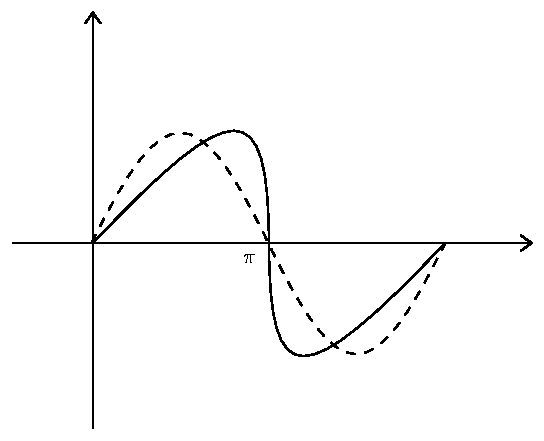
\includegraphics[width=0.4\textwidth]{tikz/burgers-sin.pdf}
    \caption{Burgers方程使用初值 $u_0(x) = \sin(x)$,随着时间演化,解会在 $x=\pi$ 位置出现间断} \label{fig:burgers-sin}
\end{figure}

\section{弱解}

对于双曲守恒律方程,即使初值足够光滑,解也可能随着时间演化产生间断等复杂结构,在间断位置显然不连续、不可导,不可能满足守恒律方程微分形式,
此时无法找到满足要求的解(经典解,古典解),或者说在经典解的范围内解不存在,需要扩大解的范围。

\begin{definition}[弱解定义之一]
    称函数 $u(x,t) \in L^\infty(\mathbb{R}\times(0,+\infty);\mathbb{R})$ 为双曲守恒律方程~\eqref{eq:cv-law-scalar} 的弱解,如果对于任意函数 $\varphi(x,t) \in C_0^\infty(\mathbb{R} \times \mathbb{R}^+)$,都有下式成立
    \[
        \int_{0}^{+\infty} \int_{\mathbb{R}} (u \varphi_t + f(u)\varphi_x)\,dx\,dt
        + \int_{\mathbb{R}} u(x,0)\varphi(x,0)\,dx = 0
    \]
\end{definition}

\begin{definition}[弱解定义之二]
    称函数 $u(x,t) \in L^\infty(\mathbb{R}\times(0,+\infty);\mathbb{R})$ 为双曲守恒律方程~\eqref{eq:cv-law-scalar} 的弱解,如果对于任意有界区域 $[x_L,x_R] \times [t^0,t^1] \subset \mathbb{R} \times \mathbb{R}^+$,都有下式成立
    \[
        \int_{x_L}^{x_R} u(x,t^1)\,dx - \int_{x_L}^{x_R} u(x,t^0)\,dx
        = \int_{t^0}^{t^1} f(u(x_L,t))\,dt - \int_{t^0}^{t^1} f(u(x_R,t))\,dt
    \]
\end{definition}

\begin{remark}
    可以证明对于弱解的两种定义是等价的。
    由于弱解的定义中只涉及到积分,在零测集上的修改不会产生影响,如果两个弱解仅在零测集上不同,那么我们将其视作同一个弱解。在下文表述中的逐点成立应当视作几乎处处成立。
\end{remark}

弱解是比经典解更大的概念,因为弱解对于函数的光滑性没有要求。
如果方程有一个经典解 $u \in C_0^1(\mathbb{R}\times(0,+\infty);\mathbb{R})$,那么使用分部积分就可以证明它也是弱解。

\begin{example}
    取 $f(u) = a u$,其中 $a$ 为常数。对于方程 $u_t + a u_x = 0$ 和任意初值 $u_0(x)$,
    只有在 $u_0(x)$ 具有足够光滑性时,函数 $u(x,t) = u_0(x - a t)$ 才是原方程的经典解。
    但是只要 $u_0(x)$ 具有可积性,函数 $u(x,t) = u_0(x - a t)$ 始终是原方程的弱解。
\end{example}



下面关注由分片经典解组成的函数,它可能在拼接位置没有足够的光滑性,从而不是经典解,
但是只需要在分界面上满足体现局部守恒性的Rankine-Hugoniot条件,就仍然是满足定义的弱解。

\begin{theorem}[分片弱解的刻画,Rankine-Hugoniot jump condition]\label{thm:rh-jump}
    考虑一个时空区域 $\Omega \subset \mathbb{R} \times (0,+\infty)$,假设 $\Omega$ 被一个光滑的时空曲线 $\Gamma$ 划分为两个部分:$\Omega_1,\Omega_2$,
    假设 $u_l(x,t),u_r(x,t)$ 分别是守恒律方程 $u_t + f(u)_x = 0$ 在区域 $\Omega_1,\Omega_2$ 的经典解,
    考虑定义在整个区域 $\Omega$ 上的函数
    \[
        u(x,t) =
        \left\{
        \begin{aligned}
             & u_l(x,t), & (x,t) \in \Omega_1 \\
             & u_r(x,t), & (x,t) \in \Omega_2
        \end{aligned}
        \right.
    \]
    那么 $u$ 是弱解等价于:在时空曲线 $\Gamma$ 上逐点成立
    \[
        \left[f(u_r(x)) - f(u_l(x))\right]n_x +
        \left[u_r(x) - u_l(x)\right]n_t = 0, \quad \forall\, (x,t) \in \Gamma \cap \Omega
    \]
    其中 $\bm{n}=(n_x,n_t)$ 是曲线 $\Gamma$ 在 $x$ 处的单位法向量。
\end{theorem}

\begin{proof}
    任取测试函数 $\varphi(x,t) \in C_0^\infty(\mathbb{R} \times \mathbb{R}^+;\mathbb{R})$,
    由于 $u$ 在 $\Omega_i$ 内部是连续可微的经典解,逐点成立 $u_t + f(u)_x = 0$,可以使用分部积分得到下式
    \[
        \int_{\Omega_i}[u \varphi_t + f(u) \varphi_x]\,dx\,dt
            ={}  - \int_{\Omega_i}
        [u_t \varphi + f(u)_x \varphi]\,dx\,dt
        + \int_{\partial \Omega_i}
        [ n_x f(u) + n_t u] \varphi\,ds
    \]
    对于整个区域 $\Omega$ 有
    \begin{align*}
            & \int_{\Omega}[u \cdot \varphi_t + f(u) \cdot \varphi_x]\,dx\,dt
        \\
        ={} & \sum_{i=1}^2 \left\{
        - \int_{\Omega_i}
        [u_t \cdot \varphi + f(u)_x \cdot \varphi]\,dx\,dt
        + \int_{\partial \Omega_i}
        [ n_x f(u) + n_t u]\cdot \varphi\,ds
        \right\}
        \\
        ={} & 0  - \int_{\mathbb{R}} u(x,0)\varphi(x,0)\,dx + \int_{\Gamma}[ n_x f(u_l) + n_t u_l]\cdot \varphi\,ds
        - \int_{\Gamma}[ n_x f(u_r) + n_t u_r]\cdot \varphi\,ds
    \end{align*}
    这里 $- \int_{\mathbb{R}} u(x,0)\varphi(x,0)\,dx$ 是在$t\!-\!x$上半平面的下边界(即实轴上)进行的边界积分得到的,
    此时 $n_x f(u) + n_t u = - u$;
    $\bm{n}=(n_x,n_t)$ 是时空曲线 $\Gamma$ 在 $x$ 处的单位法向量(从 $\Omega_1$ 指向 $\Omega_2$)。
    由 $\varphi$ 的任意性可知,$u$ 是弱解等价于在时空曲线 $\Gamma$ 上逐点成立
    \[
        \left[f(u_r(x)) - f(u_l(x))\right]n_x +
        \left[u_r(x) - u_l(x)\right]n_t = 0, \quad \forall\, x \in \Gamma \cap \Omega \qedhere
    \]
\end{proof}

在定理~\ref{thm:rh-jump} 的条件下,考虑一个更具体的情况:一条连续可微的时空曲线 $\Gamma: x=x(t),\, t \ge 0$ 将整个 $x-t$ 上半平面划分为左右两个区域:
\[
    \Omega_1 = \{(x,t) \mid x < x(t), t \ge 0\},
    \Omega_2 = \{(x,t) \mid x > x(t), t \ge 0\}.
\]
这两个时空区域在任意固定时刻的切片就是实轴的两个无界区间 $\Omega_1(t) =(-\infty,x(t))$ 和 $\Omega_2(t) = (x(t),+\infty)$,分界点为 $x=x(t)$。
单位法向量可以取作
\[
    \bm{n} = (n_x,n_t) = \frac{1}{\sqrt{1+(x'(t))^2}} (1,-x'(t))
\]
此时定理~\ref{thm:rh-jump} 中的条件即
\[
    \left[f(u_r(x)) - f(u_l(x))\right] - \left[u_r(x) - u_l(x)\right]x'(t) = 0, \quad \forall\, (x,t) \in \Gamma \cap \Omega
\]
如果记分界点的移动速度为 $s = x'(t)$,就可以得到 R-H 条件最常见的形式
\begin{equation}
    f(u_r) - f(u_l) = s\,(u_r - u_l).\label{eq:rh-jump}
\end{equation}


\begin{example}
    下面是 Burgers 方程的 “N波” 解:
    \[
        u(x,t) =
        \begin{cases}
            x/t, & -\sqrt{t} < x < \sqrt{t} \\
            0,   & \text{otherwise}
        \end{cases}
    \]
    “N波” 解由三片经典解组成,左右各存在一个间断 $x = \pm \sqrt{t}$,
    可以验证均满足 R-H 条件
    \[
        \frac{f(u_r) - f(u_l)}{u_r - u_l} =
        \frac{\frac{1}{2t} - 0}{- \frac{1}{\sqrt{t}} - 0} = -\frac{1}{2\sqrt{t}} = s_-,
        \qquad
        \frac{f(u_r) - f(u_l)}{u_r - u_l} =
        \frac{0 - \frac{1}{2t}}{0 - \frac{1}{\sqrt{t}}} = \frac{1}{2\sqrt{t}} = s_+,
    \]
    因此 “N波” 解是弱解。
\end{example}

\begin{remark*}
    若守恒律方程问题的初值为零,$u(x,t) = 0$ 显然是一个满足要求的弱解,
    但是上例的 “N波” 解也给出了一个弱解,这表明弱解不具有唯一性。
\end{remark*}

一个容易忽视的问题是:对守恒律方程微分形式的“等价变换”并不是真正等价的,考虑在 Burgers 方程的两侧乘以 $2u$ 并整理可得
\[
    (u^2)_t + \left(\frac{2}3 u^3\right)_x = 0, \quad
    \xrightarrow{u^2 = v} \quad
    v_t + \left(\frac{2}3 v^{3/2}\right)_x = 0
\]
这个方程看似和 Burgers 方程等价,但是分别考虑两个方程的 R-H 条件可得
\[
    s_1 = \frac{\frac12 u_r^2 - \frac12 u_l^2}{u_r - u_l}
    \quad \neq \quad
    s_2 = \frac{\frac23 u_r^3 - \frac32 u_l^3}{u_r^2 - u_l^2}
\]
两个方程对应的 R-H 条件不一致,这表明满足两个方程的弱解是不同的。
这种差异出现的原因是:对于方程微分形式的上述变形仅在 $u$ 光滑时是等价的,一旦考虑非光滑的弱解,变形就不再等价。


\begin{example}\label{eg:burgers-riemann-jump}
    对于 Burgers 方程的 Riemann 问题($u_L \neq u_R$)
    \[
        \left\{
        \begin{aligned}
            u_t + \left(\frac{u^2}2\right)_x & = 0,\quad (x,t) \in \mathbb{R} \times  \mathbb{R}^+ \\
            u(x,0)                           & =
            \begin{cases}
                u_L & x < 0 \\
                u_R & x > 0
            \end{cases}
        \end{aligned}
        \right.
    \]
    考虑具有如下形式的解:分界面以固定速度 $s$ 移动,分界面两侧保持常值
    \[
        u(x,t) =
        \begin{cases}
            u_L, & x/t < s \\
            u_R, & x/t > s
        \end{cases}
    \]
    解是弱解等价于分界面的移动速度 $s$ 满足 R-H 条件
    \[
        f(u_R)-f(u_L) = s (u_R - u_L),
        \quad \Rightarrow \quad
        s = \frac{f(u_R)-f(u_L)}{u_R - u_L} = \frac{u_L + u_R}{2}
    \]
    因此下面的分片常数解是弱解
    \[
        u(x,t) =
        \begin{cases}
            u_L, & x/t < s \\
            u_R, & x/t > s
        \end{cases},\quad s = \frac12(u_L + u_R)
    \]
    解和特征线分布如图~\ref{fig:burgers-riemann-jump} 所示。
\end{example}

\begin{figure}[htbp]
    \centering
    \begin{subfigure}[b]{0.47\textwidth}
        \centering
        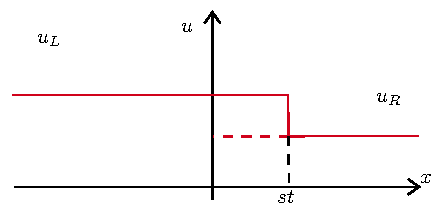
\includegraphics[width=\textwidth]{tikz/burgers-jump-1.pdf}
        \caption{$u_L > u_R$,解的形态}
    \end{subfigure}
    \begin{subfigure}[b]{0.47\textwidth}
        \centering
        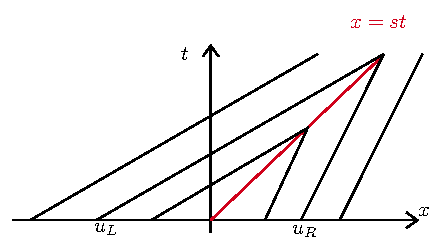
\includegraphics[width=\textwidth]{tikz/burgers-jump-1-lines.pdf}
        \caption{$u_L > u_R$,特征线汇聚}
    \end{subfigure}
    \begin{subfigure}[b]{0.47\textwidth}
        \centering
        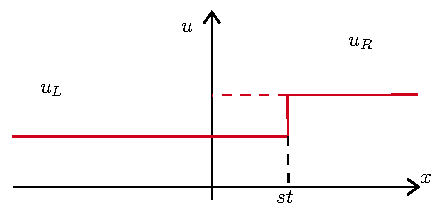
\includegraphics[width=\textwidth]{tikz/burgers-jump-2.pdf}
        \caption{$u_L < u_R$,解的形态}
    \end{subfigure}
    \begin{subfigure}[b]{0.47\textwidth}
        \centering
        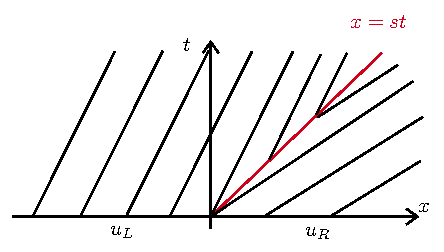
\includegraphics[width=\textwidth]{tikz/burgers-jump-2-lines.pdf}
        \caption{$u_L < u_R$,特征线发散}
    \end{subfigure}
    \caption{Burgers 方程 Riemann 问题的分片常数形式的解及其特征线分布}
    \label{fig:burgers-riemann-jump}
\end{figure}


从经典解到弱解虽然扩大了解的范围,但是弱解却不具有唯一性。
由于问题通常具有实际物理背景,必然存在唯一的解与实际的物理现象对应。
有一些方法可以在弱解范围内进一步筛选出唯一的合理的解,例如熵解和黏性解。

\section{熵解}

\begin{definition}[熵函数和熵通量]
    称函数 $\eta: \mathbb{R} \to \mathbb{R}$ 为熵函数,如果满足:$\eta \in C^2(\mathbb{R})$,并且$\eta'' \ge 0$。
    称函数 $\xi: \mathbb{R} \to \mathbb{R}$ 为对应的熵通量,如果满足 $\xi'(u) = \eta'(u) f'(u)$。
    称熵函数和对应的熵通量组成的二元组 $(\eta,\xi)$ 为一个熵对。
\end{definition}

\begin{example}
    考虑Burgers方程,例如取熵函数 $\eta(u) = \frac{1}{2} u^2$ 和熵通量 $\xi(u) = \frac{1}{3} u^3$,就满足熵对的所有要求。
    再例如取熵函数
    \[
        \eta(u) = \frac{1}{2p} u^{2p} + \frac{\alpha}2 u^2,\quad (p \in \mathbb{N}, p \ge2, \alpha > 0)
    \]
    计算可得 $\eta''(u) = (2p-1) u^{2p-2} + \alpha > 0$,代入计算可得
    \[
        \xi(u) = \frac{1}{2p+1} u^{2p+1} + \frac{\alpha}3 u^3
    \]
    任取参数 $p,\alpha$ 即可构造一组熵对 $(\eta,\xi)$ 。
\end{example}

\begin{definition}
    称方程 $u_t + f(u)_x = 0$ 的弱解 $u(x,t)$ 是熵解,如果满足:对于所有的熵对 $(\eta,\xi)$,都有如下不等式在弱形式下成立
    \[
        \eta(u)_t + \xi(u)_x \le 0.
    \]
    更具体来说,对于所有的非负测试函数 $\varphi(x,t) \in C_0^\infty(\mathbb{R} \times \mathbb{R}^+;\mathbb{R}^+)$,下式成立
    \[
        - \int_0^{+\infty} \int_{\mathbb{R}}(\eta(u) \varphi_t + \xi(u) \varphi_x) \,dx\,dt
        - \int_{\mathbb{R}} \eta(u(x,0))\varphi(x,0)\,dx \le 0
    \]
\end{definition}


显然根据定义可知,熵解一定是弱解,还需要说明的是:经典解(如果存在)一定是熵解。
假设方程有经典解 $u(x,t)$,那么直接对方程乘以 $\eta'(u)$ 可以得到
\begin{gather*}
    \eta'(u) u_t + \eta(u)' f'(u) u_x = 0 \\
    \eta(u)_t + \xi(u)_x = 0
\end{gather*}
因此也满足不等式条件。
这其实也表明熵解在足够光滑的区域可以保持等号成立,在不够光滑的区域可能导致小于号严格成立。

和弱解类似,熵解的定义不易验证,我们仍然关注由分片经典解组成的函数:它是弱解当且仅当在分界面上满足 R-H 条件;它是熵解也等价于在分界面上满足一定的条件。

\begin{theorem}[分片熵解的刻画]
    考虑定义在区域 $\Omega$ 上的由分片经典解组成的函数
    \[
        u(x,t) =
        \left\{
        \begin{aligned}
             & u_l(x,t), & (x,t) \in \Omega_1 = \{(x,t) \mid x < x(t), t \ge 0\} \\
             & u_r(x,t), & (x,t) \in \Omega_2 = \{(x,t) \mid x > x(t), t \ge 0\}
        \end{aligned}
        \right.
    \]
    其中$\Gamma: x=x(t)$ 是一条连续可微的时空曲线,$u_l(x,t)$和$u_r(x,t)$ 分别是区域 $\Omega_1,\Omega_2$ 中的经典解。
    如果 $u(x,t)$ 和分界面移动速度 $s = x'(t)$ 满足 R-H 条件~\eqref{eq:rh-jump},
    那么 $u$ 是熵解等价于:对于任意熵对 $(\eta,\xi)$,在时空曲线 $\Gamma$ 上逐点成立
    \begin{equation} \label{eq:entropy-jump}
        \left[\xi(u_r) - \xi(u_l)\right] - \left[\eta(u_r) - \eta(u_l)\right] x'(t) \le 0, \quad \forall\, (x,t) \in \Gamma \cap \Omega
    \end{equation}
\end{theorem}

\begin{proof}
    与 R-H 条件的证明过程类似。
\end{proof}

\begin{example}
    验证例~\ref{eg:burgers-riemann-jump} 提供的弱解是否是熵解。
    例如取熵对 $(\eta,\xi) = (u^2, \frac23 u^3)$,代入验证
    \begin{align*}
            & \left[\xi(u_R) - \xi(u_L)\right] - \left[\eta(u_R) - \eta(u_L)\right] x'(t)               \\
        ={} & \left(\frac23 u_R^3 - \frac23 u_L^3\right) - \left(u_R^2 - u_L^2\right) \frac{u_L + u_R}2 \\
        ={} & - \frac16 (u_L - u_R)^3
    \end{align*}
    这表明:例~\ref{eg:burgers-riemann-jump} 在 $u_L < u_R$ 时的弱解不是熵解。
    由于我们无法取遍熵对 $(\eta,\xi)$,目前仍然无法验证在 $u_L > u_R$ 时的解是熵解。
\end{example}

综上所述,经典解、熵解和弱解是三个逐渐扩大的概念,关系如图~\ref{fig:entropy-solution}。
它们之间具有严格包含的关系,即:存在不是经典解的熵解,存在不是熵解的弱解(见下文的说明)。
虽然经典解不能保证存在性,弱解不能保证唯一性,但是介于它们中间的熵解却具有存在唯一性。

\begin{theorem}
    标量双曲守恒律方程的熵解存在且唯一。
\end{theorem}

\begin{figure}[htbp]
    \centering
    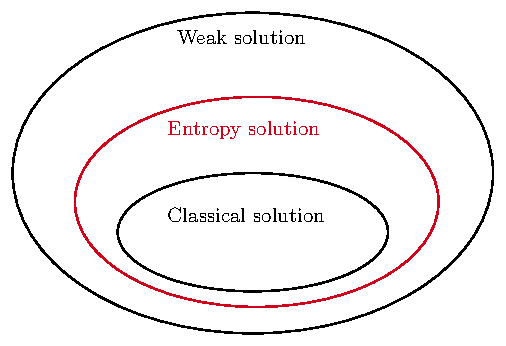
\includegraphics[width=0.5\textwidth]{tikz/entropy-solution.pdf}
    \caption{经典解、熵解和弱解的关系} \label{fig:entropy-solution}
\end{figure}

\section{黏性解}

考虑在原始的方程中加上黏性项,我们关注黏性消失后得到的极限情况,这种做法契合守恒律问题的实际物理背景。

\begin{definition}
    记 $u^{(\varepsilon)}(x,t)$ 为如下方程的解
    \begin{equation}
        u^{(\varepsilon)}_t + f(u^{(\varepsilon)})_x = \varepsilon u^{(\varepsilon)}_{xx},\quad(\varepsilon > 0) \label{eq:limit-solution}
    \end{equation}
    如果存在极限函数
    \[
        u(x,t) := \lim_{\varepsilon \to 0^+} u^{(\varepsilon)}(x,t)
    \]就称其为双曲守恒律方程的黏性解。
\end{definition}

加黏性得到的解通常具有很好的光滑性,但是随着黏性的消失,仍然可以使其收敛到存在间断的弱解。
可以证明:黏性解就是熵解。

\begin{theorem}
    对于满足~\eqref{eq:limit-solution} 的解 $u^{(\varepsilon)}(x,t)$,如果存在极限函数作为黏性解
    \[
        u(x,t) := \lim_{\varepsilon \to 0^+} u^{(\varepsilon)}(x,t)
    \]
    那么黏性解 $u(x,t)$ 就是熵解。
\end{theorem}

\begin{proof}
    $u^{(\varepsilon)}(x,t)$ 满足如下方程
    \[
        u^{(\varepsilon)}_t + f(u^{(\varepsilon)})_x = \varepsilon u^{(\varepsilon)}_{xx}
    \]
    任取熵对 $(\eta,\xi)$,在等式两侧乘以 $\eta'(u^{(\varepsilon)})$ 可得
    \begin{gather*}
        \eta'(u^{(\varepsilon)}) u^{(\varepsilon)}_t + \eta'(u^{(\varepsilon)})f(u^{(\varepsilon)})_x = \varepsilon \eta'(u^{(\varepsilon)}) u^{(\varepsilon)}_{xx}  \\
        \eta_t(u^{(\varepsilon)}) + \eta_x(u^{(\varepsilon)}) =
        \varepsilon \eta_{xx}(u^{(\varepsilon)})
        - \varepsilon \eta''(u^{(\varepsilon)})(u^{(\varepsilon)}_{x})^2
        \le \varepsilon \eta_{xx}(u^{(\varepsilon)})
    \end{gather*}
    取任意的非负测试函数 $\varphi(x,t) \in C_0^\infty(\mathbb{R} \times \mathbb{R}^+;\mathbb{R}^+)$,分部积分可得
    \[
        - \int_0^{+\infty} \int_{\mathbb{R}}(\eta(u^{(\varepsilon)}) \varphi_t + \xi(u^{(\varepsilon)}) \varphi_x) \,dx\,dt
        - \int_{\mathbb{R}} \eta(u^{(\varepsilon)}(x,0))\varphi(x,0)\,dx \le \varepsilon \int_0^{+\infty} \int_{\mathbb{R}}
        \eta(u^{(\varepsilon)}) \varphi_{xx}\,dx\,dt
    \]
    可以证明在 $\varepsilon \to 0^+$ 时,上述不等式的每一项分别收敛到下式的对应项
    \[
        - \int_0^{+\infty} \int_{\mathbb{R}}(\eta(u) \varphi_t + \xi(u) \varphi_x) \,dx\,dt
        - \int_{\mathbb{R}} \eta(u(x,0))\varphi(x,0)\,dx \le 0
    \]
    因此 $u(x,t)$ 是熵解。
\end{proof}


\section{熵条件}

由于前文中对于分片熵解的刻画条件涉及到任意的熵对,不易用于判定,我们需要更实用的熵条件。
考虑分片经典解在分界面处的间断,使用三元组 $(u_l,u_r,s)$ 表示,引入如下定义:

\begin{definition}
    称三元组 $(u_l,u_r,s)$ 为一个熵间断,如果满足 R-H 条件~\eqref{eq:rh-jump},并且对于任意熵对 $(\eta,\xi)$ 都有
    \[
        \left[\xi(u_r) - \xi(u_l)\right] - \left[\eta(u_r) - \eta(u_l)\right] s \le 0
    \]
\end{definition}

\begin{theorem}[Oleinik]
    三元组 $(u_l,u_r,s)$ 为一个熵间断,当且仅当满足 R-H 条件~\eqref{eq:rh-jump} 和 Oleinik 熵条件
    \[
        \frac{f(u_l)-f(v)}{u_l-v} \ge s \ge \frac{f(u_r)-f(v)}{u_r-v},
        \quad \forall\,v \in [\min(u_l, u_r),\,\max(u_l, u_r)]
    \]
\end{theorem}

\begin{proof}
    固定 $(x,t) \in \Gamma \cap \Omega$,任取熵对 $(\eta,\xi)$,条件~\eqref{eq:entropy-jump} 等价于
    \[
        0 \ge{}  \int_{u_l}^{u_r} \left(\xi'(v) - s\, \eta'(v)\right) \,dv
        = \int_{u_l}^{u_r} \eta'(v) \left(f'(v) - s\right) \,dv
    \]
    使用分部积分可以导出下面两个不等式
    \begin{gather*}
        \int_{u_l}^{u_r} \eta''(v) \big[ f(v) - f(u_r) - s(v - u_r) \big] \,dv \ge 0 \\
        \int_{u_l}^{u_r} \eta''(v) \big[ f(v) - f(u_l) - s(v - u_l) \big] \,dv \ge 0
    \end{gather*}
    代入 $s = \frac{f(u_r)-f(u_l)}{u_r - u_l}$ 可知这两个式子是等价的,但是这里使用两种形式便于分别证明两个不等关系。
    因为熵函数 $\eta$ 的任意性以及始终有 $\eta'' \ge 0$,必然有
    \begin{gather*}
        (u_r - u_l) \big[ f(v) - f(u_r) - s(v - u_r) \big] \ge 0,\quad \forall\,v \in [\min(u_l, u_r),\,\max(u_l, u_r)] \\
        (u_r - u_l) \big[ f(v) - f(u_l) - s(v - u_l) \big] \ge 0,\quad \forall\,v \in [\min(u_l, u_r),\,\max(u_l, u_r)]
    \end{gather*}
    整理可得
    \begin{gather*}
        (u_r - u_l)(u_r - v) \left[ s - \frac{f(u_r)-f(v)}{u_r-v} \right] \ge 0,\quad \forall\,v \in [\min(u_l, u_r),\,\max(u_l, u_r)] \\
        (u_r - u_l)(v - u_l) \left[ \frac{f(u_l)-f(v)}{u_l-v} - s\right] \ge 0,\quad \forall\,v \in [\min(u_l, u_r),\,\max(u_l, u_r)]
    \end{gather*}
    无论 $u_l$ 和 $u_r$ 的大小关系如何,对于 $v \in [\min(u_l, u_r),\,\max(u_l, u_r)]$,始终有
    \[
        (u_r - u_l)(u_r - v) \ge 0, \quad (u_r - u_l)(v - u_l) \ge 0
    \]
    因此得证。
\end{proof}

需要结合函数图像来理解 Oleinik 熵条件:定义 $g(u) = f(u_l) + s(u - u_l) = f(u_r) + s(u - u_r)$,也就是过 $(u_l,f(u_l))$ 和 $(u_r,f(u_r))$ 两点的直线,那么 Oleinik 熵条件可以解释为(如图~\ref{fig:oleinik-condition})

\begin{itemize}
    \item 如果 $u_l < u_r$,要求在 $[u_l,u_r]$ 范围内,曲线 $y=f(u)$ 始终在两点连线 $y=g(u)$ 的上方或重合;
    \item 如果 $u_l > u_r$,要求在 $[u_r,u_l]$ 范围内,曲线 $y=f(u)$ 始终在两点连线 $y=g(u)$ 的下方或重合;
\end{itemize}

\begin{figure}[htbp]
    \centering
    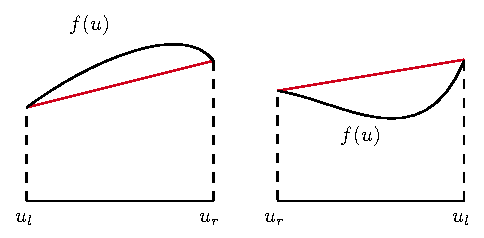
\includegraphics[width=0.6\textwidth]{tikz/oleinik-condition.pdf}
    \caption{Oleinik 熵条件的解释} \label{fig:oleinik-condition}
\end{figure}

对 Oleinik 熵条件中的不等式,直接令 $u \to u_l,u_r$ 可得
\[
    f'(u_l) \ge s \ge f'(u_r)
\]
这个条件被称为 Osher 熵条件。
对于任意可微的 $f(u)$,Osher 熵条件是 Oleinik 熵条件的推论,并不是充要条件,但是如果要求 $f'' \neq 0$,那么两者就是等价的。

由于 $f'(u)$ 的物理意义是物质的移动速度,$s$ 是分界面的移动速度,Osher 熵条件要求:
\begin{itemize}
    \item 左侧物质的移动速度大于等于分界面的移动速度;
    \item 分界面的移动速度大于等于右侧物质的移动速度。
\end{itemize}
由于 $f'(u)$ 在 $x\!-\!t$ 平面上具有明确的几何意义--对应特征线的斜率倒数,Osher 熵条件还可以结合特征线的分布来解释:
\begin{itemize}
    \item 只有间断两侧特征线不断向时空分界面汇聚(或平行),对应的间断解才可能是熵解。
    \item 如果间断两侧特征线呈现发散趋势,那么对应的间断解即使满足局部守恒性,仍然是不合理的。
\end{itemize}


\begin{example}
    对于 Burgers 方程,由于 $f''(u) = 1 >0$ 严格凸,Osher 熵条件是充要的。
    使用 Osher 熵条件检查例~\ref{eg:burgers-riemann-jump} 提供的弱解:
    \begin{gather*}
        f'(u_L) \ge s = \frac{f(u_R)-f(u_L)}{u_R - u_L} \ge f'(u_R), \\
        \Rightarrow \quad u_L \ge s = \frac{u_L + u_R}2 \ge u_R \\
        \Rightarrow \quad u_L \ge u_R
    \end{gather*}
    因此当且仅在 $u_L \ge u_R$ 时,例~\ref{eg:burgers-riemann-jump} 提供的解是熵解。
\end{example}


\section{激波、接触间断和稀疏波}

现在对由分片经典解组成的熵解的形态进行更具体的刻画,其中存在三类典型结构:激波、接触间断和稀疏波,
分别对应着特征线的三种趋势:汇聚,平行,发散。

\begin{definition}
    对于熵间断 $(u_l,u_r,s)$,将其分为两类:
    \begin{itemize}
        \item 称为激波,如果至少存在一个熵对 $(\eta,\xi)$,使得
              \[
                  \left[\xi(u_r) - \xi(u_l)\right] - \left[\eta(u_r) - \eta(u_l)\right] s < 0
              \]
        \item 称为接触间断,如果对于任意熵对 $(\eta,\xi)$,都有
              \[
                  \left[\xi(u_r) - \xi(u_l)\right] - \left[\eta(u_r) - \eta(u_l)\right] s = 0
              \]
    \end{itemize}
\end{definition}

\begin{theorem}
    熵间断 $(u_l,u_r,s)$ 是一个接触间断等价于
    \[
        f(v) = f(u_l) + s(v - u_l) = f(u_r) + s(v - u_r), \quad v \in [\min(u_l, u_r),\,\max(u_l, u_r)]
    \]
    即 $f(u)$ 在这个范围内等于在 $(u_l,f(u_l))$ 和 $(u_r,f(u_r))$ 两点之间的连线。
\end{theorem}

\begin{proof}
    由接触间断的定义可知,$(u_l,u_r,s)$ 和 $(u_r,u_l,s)$ 都是熵间断,即两侧状态交换也不会违背熵条件。
    由 Oleinik 熵条件的图像解释可知,$f(u)$ 既要求在两点之间连线的上方或重合,也要求在两点之间连线的下方或重合,因此 $f(u)$ 必然和两点之间连线完全重合。
\end{proof}

这表明产生接触间断的条件是曲线 $y=f(u)$ 在某一个区间内是直线。
考虑从特征线的角度理解:对于接触间断 $(u_l,u_r,s)$,由于 $f'$ 在 $[\min(u_l, u_r),\,\max(u_l, u_r)]$ 是常值,因此有
\[
    f'(u_l) = s = f'(u_r)
\]
这表明:在 $x\!-\!t$ 平面上,接触间断的两侧特征线平行,并且和时空区域的分界面也平行。从物理角度来说,这表明接触间断的两侧实际并没有发生物质交换,激波的两侧则发生了物质交换。
考虑两个具体的方程:
\begin{itemize}
    \item 对于 Burgers 方程,$f(u) = \frac12 u^2$,由于不存在直线片段,因此产生的熵间断只可能是激波;
    \item 对于线性方程,$f(u) = a u$($a$ 为常数),由于本身就是直线,因此产生的熵间断只可能是接触间断。
\end{itemize}

\begin{example}
    考虑 $f(u) = a u$($a$ 为常数),那么特征线为一组平行的直线。对于初值 $u_0(x) = \chi_{[m,n]}(x)$,由特征线的走向可以直接得到解
    \[
        u(x,t) = u_0(x - a t) = \chi_{[m+at,n+at]}(x)
    \]
    存在两处间断:$(0,1,a)$ 和 $(1,0,a)$,显然均满足 R-H 条件和 Oleinik 熵条件,因此是熵间断,
    根据上述命题可知,这两个熵间断都是接触间断。
\end{example}


重新考虑守恒律方程的微分形式
\[
    u_t + f(u)_x = 0
\]
如果 $f'$ 局部可逆,不妨设 $(f')^{-1}$ 可以定义在区间 $[s^{(l)},s^{(r)}]$,那么可以构造如下形式的(局部)解
\[
    u(x,t) = (f')^{-1}\left(\frac{x-x_0}{t}\right), \quad  x \in [x_0 + s^{(l)}t ,\, x_0 +s^{(r)} t ]
\]
其中 $x_0$ 是任意给定的起点,定义区间是随时间演化逐渐扩大的区间 $[x_0 + s^{(l)}t ,\, x_0 + s^{(r)} t]$,在两端的值记作
\[
    u^{(l)} = (f')^{-1}(s^{(l)}), \quad
    u^{(r)} = (f')^{-1}(s^{(r)})
\]
在 $x\!-\!t$ 平面内,解的所有特征线位于从 $(x_0,0)$ 发出的一个扇形区域
\[
    S = \{(x,t) \mid s^{(l)} t \le x - x_0 \le s^{(r)} t \}
\]
特征线呈现发散趋势,并且特征线斜率从一侧到另一侧连续过渡,如图~\ref{fig:rarefaction}。

\begin{figure}[htbp]
    \centering
    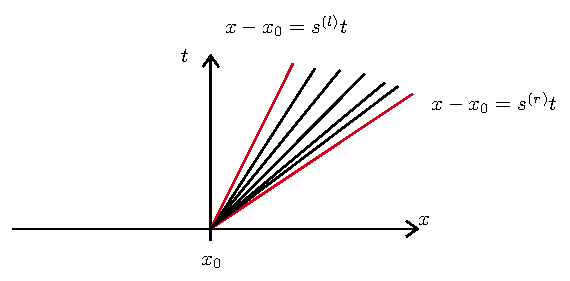
\includegraphics[width=0.6\textwidth]{tikz/rerafaction.pdf}
    \caption{稀疏波对应的特征线分布} \label{fig:rarefaction}
\end{figure}

由构造过程可知,这个局部解具有自相似性,并且在定义区间内是连续的,可以直接验证在区间内部是满足守恒律方程的微分形式
\begin{align*}
    u_t + f(u)_x ={} &
    \frac{1}{f''(u)} (f''(u) u_t + f'(u) f''(u) u_x)                                                                                                 \\
    ={}              & \frac{1}{f''(u)} \left[ \partial_t f'(u) + \partial_x \left( \frac{(f'(u))^2}2 \right)\right]                                 \\
    ={}              & \frac{1}{f''(u)} \left[  \partial_t \left( \frac{x-x_0}{t} \right) + \partial_x \left( \frac{(x-x_0)^2}{2t^2} \right) \right] \\
    ={}              & \frac{1}{f''(u)} \left( - \frac{x-x_0}{t^2} + \frac{x-x_0}{t^2} \right) = 0
\end{align*}

\begin{definition}
    上文构造的(局部)经典解称为(从 $x=x_0$ 发出的)稀疏波。
\end{definition}

\begin{remark*}
    稀疏波解的构造受限于 $f'$ 的局部可逆性,如果 $f'$ 是全局可逆的(例如 $f$ 严格凸),
    那么定义稀疏波解时的参数 $s^{(l)}$ 和 $s^{(r)}$ 可以在 $f'(u)$ 的值域中自由选取。
\end{remark*}

\begin{example}
    考虑 $f(u) = \frac12 u^2$,$f'(u) = u$ 全局可逆,可以构造稀疏波解
    \[
        u(x,t) = (f')^{-1}\left(\frac{x-x_0}{t}\right) = \frac{x-x_0}{t}
    \]
\end{example}

\begin{example}
    考虑 $f(u) = \frac14 u^4$,$f'(u) = u^3$ 全局可逆,可以构造稀疏波解
    \[
        u(x,t) = (f')^{-1}\left(\frac{x-x_0}{t}\right) = \left(\frac{x-x_0}{t}\right)^{\frac13}
    \]
\end{example}

\section{Riemann 问题的熵解}

对于一般的双曲守恒律方程的 Riemann 问题($u_L \neq u_R$)
\[
    \left\{
    \begin{aligned}
        u_t + f(u)_x & = 0,\quad (x,t) \in \mathbb{R} \times  \mathbb{R}^+ \\
        u(x,0)       & =
        \begin{cases}
            u_L & x < 0 \\
            u_R & x > 0
        \end{cases}
    \end{aligned}
    \right.
\]
熵解的显式表达形式过于复杂,但是我们可以给出它的构造。为了描述解的构造过程,我们必须使用一些简化表述,考虑两个状态之间的连接:
\begin{enumerate}
    \item 称左右状态 $u^{(l)}$ 和 $u^{(r)}$ 通过(从$x=0$发出的)稀疏波连接,对应的解为
          \[
              u(x,t) = (f')^{-1}\left(\frac{x}{t}\right), \quad  x \in [f'(u^{(l)}) t ,\, f'(u^{(r)}) t ]
          \]
          这要求 $f'(u^{(l)}) < f'(u^{(r)})$ 以及 $f'$ 在 $[\min(u^{(l)},u^{(r)}),\,\max(u^{(l)},u^{(r)})]$ 是局部可逆的。
          这两个条件也可以表述为:

          \begin{enumerate}
              \item 若 $u^{(l)} < u^{(r)}$,要求 $f'$ 在 $[u^{(l)},u^{(r)}]$ 严格单调增,亦即 $\{ (u,y) \mid y \ge f(u),\, u \in [u^{(l)},u^{(r)}]\}$ 是凸集,并且 $f(u)$ 在这个范围内不是线性的;
              \item 若 $u^{(l)} > u^{(r)}$,要求 $f'$ 在 $[u^{(r)},u^{(l)}]$ 严格单调减,亦即 $\{ (u,y) \mid y \le f(u),\, u \in [u^{(r)},u^{(l)}]\}$ 是凸集,并且 $f(u)$ 在这个范围内不是线性的。
          \end{enumerate}

    \item 称左右状态 $u^{(l)}$ 和 $u^{(r)}$ 通过激波或接触间断连接,对应的解为
          \[
              u(x,t) =
              \begin{cases}
                  u^{(l)}, & x/t < s \\
                  u^{(r)}, & x/t > s
              \end{cases}, \quad s = \frac{f(u^{(r)})-f(u^{(l)})}{u^{(r)} - u^{(l)}}
          \]
          分界面位置为 $x = x(t) = s\,t$,需要满足 Oleinik 熵条件
          \[
              \frac{f(u^{(l)})-f(v)}{u^{(l)}-v} \ge s \ge \frac{f(u^{(r)})-f(v)}{u^{(r)}-v},
              \quad \forall\,v \in [\min(u^{(l)}, u^{(r)}),\,\max(u^{(l)}, u^{(r)})]
          \]
          也可以表述为:记连接 $(u^{(l)},f(u^{(l)}))$ 和 $(u^{(r)},f(u^{(r)}))$ 两点的直线为 $g(u) = f(u^{(l)}) + s(u - u^{(l)})$,那么
          \begin{enumerate}
              \item 若 $u^{(l)} < u^{(r)}$,要求 $g(u) \le f(u)$ 在 $[u^{(l)},u^{(r)}]$ 成立,亦即 $\{ (u,y) \mid y \ge g(u),\, u \in [u^{(l)},u^{(r)}]\}$ 是 $\{ (u,y) \mid y \ge f(u),\, u \in [u^{(l)},u^{(r)}]\}$ 的凸包;
              \item 若 $u^{(l)} > u^{(r)}$,要求 $g(u) \ge f(u)$ 在 $[u^{(r)},u^{(l)}]$ 成立,亦即 $\{ (u,y) \mid y \le g(u),\, u \in [u^{(r)},u^{(l)}]\}$ 是 $\{ (u,y) \mid y \le f(u),\, u \in [u^{(r)},u^{(l)}]\}$ 的凸包。
          \end{enumerate}
\end{enumerate}
然后考虑三个点之间的状态连接:对于左状态 $u^{(l)}$,中状态 $u^{(m)}$ 和右状态 $u^{(r)}$:
\begin{enumerate}
    \item 如果均使用激波或接触间断相连,那么在考虑满足两个状态连接的要求之后,可以推出:左状态可以直接和右状态使用激波或接触间断相连,无需中间状态;
    \item 如果均使用稀疏波相连,那么在考虑满足两个状态连接的要求之后,同样可以推出:左状态可以直接和右状态使用稀疏波相连,无需中间状态;
    \item 如果左状态和中间状态使用激波或接触间断连接,而中间状态到右状态使用稀疏波相连,那么由稀疏波的定义区间和分界面位置可以推出
          \[
              f'(u^{(m)}) = \frac{f(u^{(m)}) - f(u^{(l)})}{u^{(m)} - u^{(l)}}
          \]
          从图像角度来解释,这表明在公共点 $u^{(m)}$,$f(u)$ 的曲线和激波或接触间断对应的直线需要满足相切关系。
    \item 如果左状态和中间状态使用稀疏波连接,而中间状态到右状态使用激波或接触间断相连,同理
          \[
              f'(u^{(m)}) = \frac{f(u^{(r)}) - f(u^{(m)})}{u^{(r)} - u^{(m)}}
          \]
\end{enumerate}

寻找 Riemann 问题的熵解的问题可以转换为:寻找一个单调的状态序列来连接左右初值状态 $u_L$ 和 $u_R$,不妨记作
\begin{align*}
                   & u_L = u^{(1)} < u^{(2)} < \cdots < u^{(k-1)} < u^{(k)} = u_R \\
    \text{or}\quad & u_L = u^{(1)} > u^{(2)} > \cdots > u^{(k-1)} > u^{(k)} = u_R
\end{align*}
如果相邻状态 $u^{(i)}$ 和 $u^{(i+1)}$ 均可以通过激波、接触间断或稀疏波相连,满足前文中讨论的所有条件,
那么就可以得到一个符合要求的熵解,也就是唯一的熵解。

因为我们已经将不同状态之间可以连接的条件全都转换为了图像角度的要求,可以自然诱导出使用凸包来寻找单调状态序列的方法:
对于左右初值 $u_L$ 和 $u_R$ 的 Riemann 问题,引入辅助函数 $g(u)$:
\begin{enumerate}
    \item 若 $u_L < u_R$,定义 $g(u)$,使得$\{ (u,y) \mid y \ge g(u),\, u \in [u_L,u_R]\}$ 是 $\{ (u,y) \mid y \ge f(u),\, u \in [u_L,u_R]\}$ 的凸包;
    \item 若 $u_L > u_R$,定义 $g(u)$,使得$\{ (u,y) \mid y \le g(u),\, u \in [u_L,u_R]\}$ 是 $\{ (u,y) \mid y \le f(u),\, u \in [u_L,u_R]\}$ 的凸包。
\end{enumerate}
由凸包的构造过程可知,$g(u)$ 通常可以使用分段函数表示,不妨记作
\[
    g(u) = g^{(i)}(u), \quad u \in [\min(u^{(i)},u^{(i+1)}),\max(u^{(i)},u^{(i+1)})],\quad i=1,\dots,k-1
\]
并且 $g^{(i)}(u)$ 只有三种互异的情况:
\begin{enumerate}
    \item $g^{(i)}(u) = f(u)$,并且在这个范围内是线性的;
    \item $g^{(i)}(u) = f(u)$,并且在这个范围内不是线性的;
    \item $g^{(i)}(u) \neq f(u)$,而是连接两个端点的直线
          \[
              g^{(i)}(u) = f(u^{(i)}) + s(u - u^{(i)}),\quad s = \frac{f(u^{(i+1)})-f(u^{(i)})}{u^{(i+1)} - u^{(i)}}
          \]
          此时两端点如果不是边界点 $u_L,u_R$,必然满足相切关系 $s = f'(u^{(i)})$,$s = f'(u^{(i+1)})$。
\end{enumerate}
容易验证,通过 $g(u)$ 的分段函数表示自然得到的单调状态序列 $\{u^{(i)}\}$ 满足所有要求。
因此,我们可以给出一般情况下的熵解构造。
\begin{theorem}
    对于一般的 $f$,Rimann 问题的熵解可以通过如下方式构造:
    基于 $u_L$ 与 $u_R$ 的大小关系构造 $f(u)$ 相关的凸包函数 $g(u)$,由 $g(u)$ 的分段表示诱导产生一组状态
    \begin{align*}
                       & u_L = u^{(1)} < u^{(2)} < \cdots < u^{(k-1)} < u^{(k)} = u_R \\
        \text{or}\quad & u_L = u^{(1)} > u^{(2)} > \cdots > u^{(k-1)} > u^{(k)} = u_R
    \end{align*}
    对于相邻状态 $u^{(i)}$ 和 $u^{(i+1)}$:
    \begin{enumerate}
        \item 如果 $g^{(i)}(u) = f(u)$,并且在这个范围内是线性的,那么两个状态应当使用接触间断相连;
        \item 如果 $g^{(i)}(u) = f(u)$,并且在这个范围内不是线性的,那么两个状态应当使用稀疏波相连;
        \item 如果 $g^{(i)}(u) \neq f(u)$,而是连接两个端点的直线,那么两个状态应当使用激波相连。
    \end{enumerate}
    这样得到的解就是 Riemann 问题的熵解。

\end{theorem}

由于一般情况的解的组成比较复杂,难以给出显式的表达形式,但是我们可以考虑一些简单的例子,图~\ref{fig:entropy-solution-general} 展示了几种典型情况,
例如左上图(稀疏波—激波)对应的解为:
\[
    u(x,t) ={}
    \begin{cases}
        u_L,            & x/t < f'(u_L)                       \\
        (f')^{-1}(x/t), & f'(u_L) \le x/t \le f'(u^{(2)}) = s \\
        u_R,            & x/t > f'(u^{(2)}) = s
    \end{cases}
    ,\quad
    s := \frac{f(u_R) - f(u^{(2)})}{u_R - u^{(2)}}
\]
左下图(激波—稀疏波)对应的解的显式表达为:
\[
    u(x,t) ={}
    \begin{cases}
        u_L,            & x/t < f'(u^{(2)}) = s               \\
        (f')^{-1}(x/t), & s = f'(u^{(2)}) \le x/t \le f'(u_R) \\
        u_R,            & x/t > f'(u_R)
    \end{cases}
    ,\quad
    s := \frac{f(u^{(2)}) - f(u_L)}{u^{(2)} - u_L}
\]
图~\ref{fig:entropy-solution-general-2} 给出了一种更复杂的情况:稀疏波—激波—稀疏波,对应的解为:
\[
    u(x,t) ={}
    \begin{cases}
        u_L,            & x/t < f'(u_L)                       \\
        (f')^{-1}(x/t), & f'(u_L) \le x/t < f'(u^{(2)}) = s   \\
        (f')^{-1}(x/t), & s = f'(u^{(3)}) \le x/t \le f'(u_R) \\
        u_R,            & x/t > f'(u_R)
    \end{cases}
    ,\quad
    s := \frac{f(u^{(3)}) - f(u^{(2)})}{u^{(3)} - u^{(2)}}
\]

\begin{figure}[htbp]
    \centering
    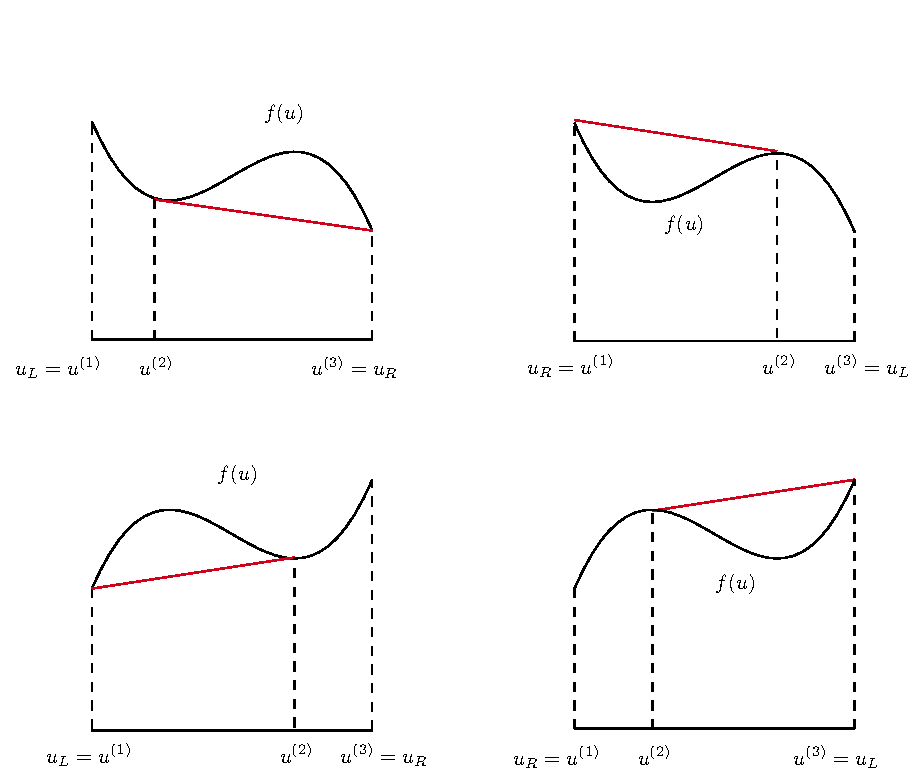
\includegraphics[width=\textwidth]{tikz/entropy-solution-general.pdf}
    \caption{对于一般的 $f$,Riemann 问题的几种熵解结构示意:左上图和右上图代表稀疏波—激波,左下图和右下图代表激波—稀疏波。}
    \label{fig:entropy-solution-general}
\end{figure}

\begin{figure}[htbp]
    \centering
    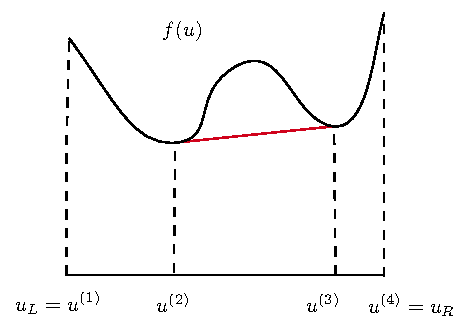
\includegraphics[width=.6\textwidth]{tikz/entropy-solution-general-2.pdf}
    \caption{对于一般的 $f$,Riemann 问题的一种熵解结构示意:稀疏波—激波—稀疏波。}
    \label{fig:entropy-solution-general-2}
\end{figure}


在一般性结论的基础上,考虑 $f'' > 0$ 严格凸的情形,根据上述定理:
\begin{enumerate}
    \item 若 $u_L < u_R$,那么 $g(u) = f(u)$,只存在两个状态 $u_L$ 和 $u_R$,并且必然通过稀疏波相连;
    \item 若 $u_L > u_R$,那么 $g(u) = f(u_L) + s(u - u_L)$ 为两点连线,只存在两个状态 $u_L$ 和 $u_R$,并且必然通过激波相连。
\end{enumerate}
由于此时熵解的构造非常简单,可以直接给出熵解的显式表达。

\begin{theorem}
    对于 $f$ 严格凸的情况,Rimann 问题的熵解为:
    \begin{enumerate}
        \item 如果 $u_L < u_R$,$u(x,t)$ 是一个(从$x=0$发出的)稀疏波,具体为
              \[
                  u(x,t) ={}
                  \begin{cases}
                      u_L,            & x/t < f'(u_L)               \\
                      (f')^{-1}(x/t), & f'(u_L) \le x/t \le f'(u_R) \\
                      u_R,            & x/t > f'(u_R)
                  \end{cases}
              \]
        \item 如果 $u_L > u_R$,$u(x,t)$ 是一个激波,具体为
              \[
                  u(x,t) =
                  \begin{cases}
                      u_L, & x/t < s \\
                      u_R, & x/t > s
                  \end{cases},\quad s = \frac{f(u_R)-f(u_L)}{u_R - u_L}
              \]
    \end{enumerate}
    如图~\ref{fig:entropy-solution-convex} 所示。
\end{theorem}

\begin{figure}[htbp]
    \centering
    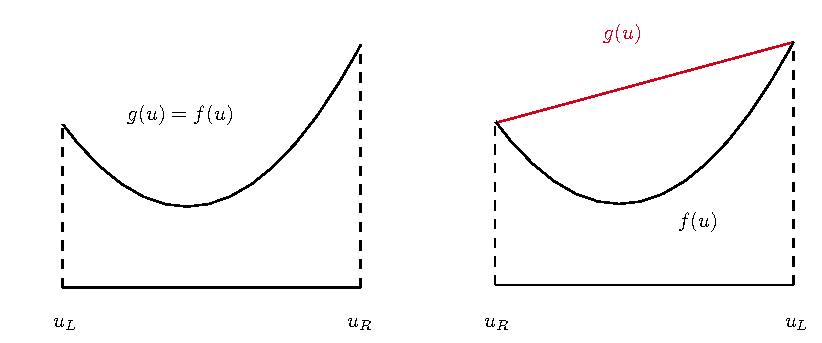
\includegraphics[width=.9\textwidth]{tikz/entropy-solution-convex.pdf}
    \caption{对于严格凸的 $f$,Riemann 问题的熵解结构示意,左图代表稀疏波,右图代表激波。} \label{fig:entropy-solution-convex}
\end{figure}

\begin{example}
    考虑一个典型的 $f$ 非凸非凹的情况—— Buckley-Leverett 方程,对应的 $f(u)$ 具体为
    \[
        f(u) = \frac{u^2}{u^2 + a(1-u)^2}.
    \]
    其中参数 $a > 0$ 给定,通常只关注 $u \in [0,1]$ 的情况。
    我们考虑两个 Riemann 问题:
    \begin{enumerate}
        \item $u_L = 0$,$u_R = 1$;
        \item $u_L = 1$,$u_R = 0$。
    \end{enumerate}
    两种情况下的熵解结构均为稀疏波—激波,具体表达式为
    \[
        u(x,t) ={}
        \begin{cases}
            u_L,            & x/t < f'(u_L)                       \\
            (f')^{-1}(x/t), & f'(u_L) \le x/t \le f'(u^{(2)}) = s \\
            u_R,            & x/t > f'(u^{(2)}) = s
        \end{cases}
        ,\quad
        s := \frac{f(u_R) - f(u^{(2)})}{u_R - u^{(2)}}
    \]
    中间状态 $u^{(2)}$ 的具体值可以通过如下方程解出
    \[
        f'(u^{(2)}) = \frac{f(u_R) - f(u^{(2)})}{u_R - u^{(2)}}
    \]
    熵解结构以及解的形态如图~\ref{fig:buckley-leverett-riemann} 所示。
\end{example}

\begin{figure}[htbp]
    \centering
    \begin{subfigure}[b]{\textwidth}
        \centering
        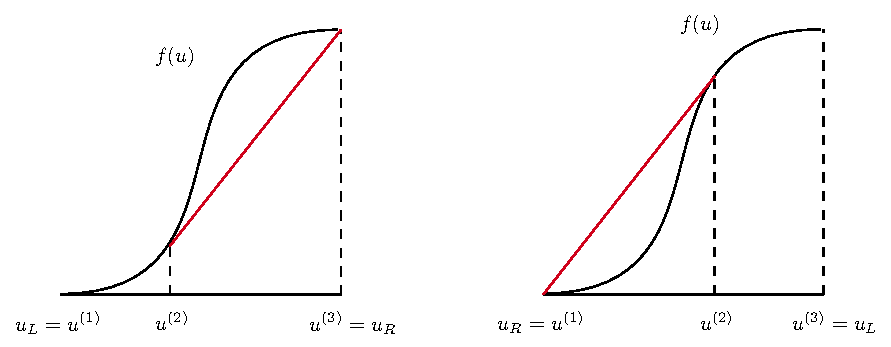
\includegraphics[width=.9\textwidth]{tikz/buckley-leverett-riemann.pdf}
    \end{subfigure}
    \begin{subfigure}[b]{\textwidth}
        \centering
        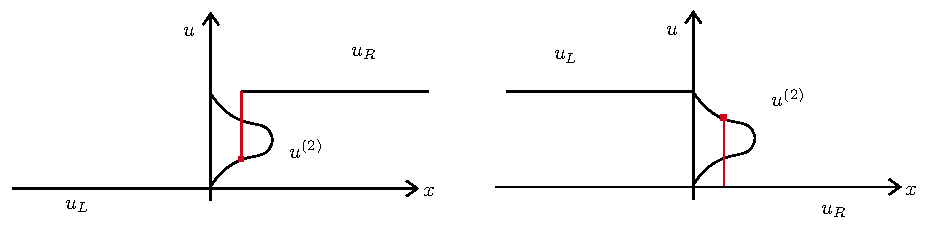
\includegraphics[width=\textwidth]{tikz/buckley-leverett-riemann-plot.pdf}
    \end{subfigure}
    \caption{Buckley-Leverett 方程 Riemann 问题的熵解结构以及解的形态。} \label{fig:buckley-leverett-riemann}
\end{figure}


我们关注 Riemann 问题在分界面 $x=0$ 的解 $u(0,t)$ 以及 $f(u(0,t))$ 的值,需要结合图像进行分类讨论:
\begin{enumerate}
    \item $u_L < u_R$ 时,假设 $f(u)$ 在 $[u_L,u_R]$ 存在唯一的最小值点 $\widetilde{u}_m$,
          它必然也是 $g(u)$ 的最小值点
          \begin{enumerate}
              \item 如果 $\widetilde{u}_m$ 位于某个稀疏波中,那么由于 $f'(\widetilde{u}_m) = 0$,必有 $u(0,t) = \widetilde{u}_m$;
                    否则 $\widetilde{u}_m$ 必然处于激波或接触间断的一端,并且 $\widetilde{u}_m$ 必须为 $u_L$ 或 $u_R$;
              \item 如果 $\widetilde{u}_m = u_L$,这段对应的斜率(间断移动速度)必然大于0,必有 $u(0,t) = u_L = \widetilde{u}_m$;
              \item 如果 $\widetilde{u}_m = u_R$,这段对应的斜率(间断移动速度)必然小于0,必有 $u(0,t) = u_R = \widetilde{u}_m$。
          \end{enumerate}
    \item $u_L > u_R$ 时,假设 $f(u)$ 在 $[u_L,u_R]$ 存在唯一的最大值点 $\widetilde{u}_M$;
          它必然也是 $g(u)$ 的最大值点
          \begin{enumerate}
              \item 如果 $\widetilde{u}_m$ 位于某个稀疏波中,那么由于 $f'(\widetilde{u}_M) = 0$,必有 $u(0,t) = \widetilde{u}_M$;
                    否则 $\widetilde{u}_M$ 必然处于激波或接触间断的一端,并且 $\widetilde{u}_M$ 必须为 $u_L$ 或 $u_R$;
              \item 如果 $\widetilde{u}_M = u_L$,这段对应的斜率(间断移动速度)必然大于0,必有 $u(0,t) = u_L = \widetilde{u}_M$;
              \item 如果 $\widetilde{u}_M = u_R$,这段对应的斜率(间断移动速度)必然小于0,必有 $u(0,t) = u_R = \widetilde{u}_M$。
          \end{enumerate}
\end{enumerate}
整理可得
\[
    u(0,t) =
    \begin{cases}
        \text{argmin}_{[u_L,u_R]} f(u), & u_L < u_R \\
        \text{argmax}_{[u_R,u_L]} f(u), & u_L > u_R
    \end{cases}
\]
如果有多个最值点,那么会在 $x=0$ 位置形成固定不动的激波或接触间断,此时 $u(0,t)$ 无法定义。
但是无论最值点是否唯一,都不影响 $f(u(0,t))$ 的取值
\[
    f(u(0,t)) =
    \begin{cases}
        \text{min}_{[u_L,u_R]} f(u), & u_L < u_R \\
        \text{max}_{[u_R,u_L]} f(u), & u_L > u_R
    \end{cases}
\]
这样就得到了著名的 Godunov flux:
\[
    f^{God}(u_L,u_R) =
    \begin{cases}
        \text{min}_{[u_L,u_R]} f(u), & u_L \le u_R \\
        \text{max}_{[u_R,u_L]} f(u), & u_L > u_R
    \end{cases}
\]

\section{近似 Riemann 解}

在数值格式中,我们通常希望近似求解 Riemann 问题,做法是直接假设 Riemann 问题具有某种典型的结构,然后联列条件求解。

假定左右状态使用激波相连,那么
\[
    u(0,t) =
    \begin{cases}
        u_L, & s \ge 0 \\
        u_R. & s < 0
    \end{cases},
    \quad
    f(u(0,t)) =
    \begin{cases}
        f(u_L), & s \ge 0 \\
        f(u_R). & s < 0
    \end{cases},
    \quad
    s = \frac{f(u_R)-f(u_L)}{u_R - u_L}
\]
这样就得到了 Roe flux:
\[
    f^{Roe}(u_L,u_R) =
    \begin{cases}
        f(u_L), & s \ge 0 \\
        f(u_R). & s < 0
    \end{cases},
    \quad
    s = \frac{f(u_R)-f(u_L)}{u_R - u_L}
\]

假定左右状态使用稀疏波相连,那么
\[
    u(0,t) =
    \begin{cases}
        \text{argmin}_{[u_L,u_R]} f(u), & u_L < u_R \\
        \text{argmax}_{[u_R,u_L]} f(u), & u_L > u_R
    \end{cases}
\]
由几何关系可得 $f(u(0,t))$ 满足
\begin{gather*}
    \int_{u_L}^{u_R} |f'(u)|\,du = f(u_L) - f(u(0,t)) + f(u_R) - f(u(0,t)) \\
    f(u(0,t)) = \frac{f(u_L) + f(u_R)}2 - \frac12 \int_{u_L}^{u_R} |f'(u)|\,du
\end{gather*}
这样就得到了 Engquist-Osher flux:
\[
    f^{EO}(u_L,u_R) = \frac{f(u_L) + f(u_R)}2 - \frac12 \int_{u_L}^{u_R} |f'(u)|\,du
\]

假定左右状态使用两个激波相连,不妨记中间状态为 $u_M$,记两个激波速度为 $s_1 < s_2$,那么必然满足 R-H 条件
\begin{align*}
    f(u_M) - f(u_L) & = s_1(u_M - u_L) \\
    f(u_R) - f(u_M) & = s_2(u_R - u_M)
\end{align*}
理想情况下,$(s_1,s_2,u_M)$ 应当同时满足这两个等式,此时
\[
    u(0,t)  =
    \begin{cases}
        u_L, & 0 \le s_1     \\
        u_M. & s_1 < 0 < s_2 \\
        u_R. & s_2 \le 0
    \end{cases},
    \quad
    f(u(0,t))  =
    \begin{cases}
        f(u_L), & 0 \le s_1     \\
        f(u_M). & s_1 < 0 < s_2 \\
        f(u_R). & s_2 \le 0
    \end{cases},
\]
由于非线性方程组难以求解,实践中通常直接使用左右状态估计 $s_1$ 和 $s_2$,例如
\[
    s_1 = \min(f'(u_L),f'(u_R)),\quad
    s_2 = \max(f'(u_L),f'(u_R)).
\]
然后代入计算近似值
\begin{gather*}
    \tilde{u}_M := \frac{s_2 u_R - s_1 u_L + f(u_L) - f(u_R)}{s_2 - s_1}\\
    \tilde{f}_M := \frac{s_2 f(u_L) - s_1 f(u_R) + s_1 s_2(u_R - u_L)}{s_2 - s_1}
\end{gather*}
这样就得到了 HLL flux:
\[
    f^{HLL}(u_L,u_R) =
    \begin{cases}
        f(u_L),      & s_1 \ge 0     \\
        \tilde{f}_M. & s_1 < 0 < s_2 \\
        f(u_R).      & s_2 \le 0
    \end{cases},
    \quad
    \tilde{f}_M = \frac{s_2 f(u_L) - s_1 f(u_R) + s_1 s_2(u_R - u_L)}{s_2 - s_1}
\]

在 HLL flux 的基础上,如果我们简化两个激波速度的估计
\[
    \alpha = \max(|f'(u)|), \quad s_1 = -\alpha, \quad s_2 = \alpha
\]
即假设左右状态使用两个速度相反的激波相连,此时必然有 $s_1 \le 0 \le s_2$,代入计算可得
\[
    \tilde{f}_M = \frac{\alpha f(u_L) + \alpha f(u_R) - \alpha^2(u_R - u_L)}{2 \alpha} =
    \frac12(f(u_L) + f(u_R))  - \frac{\alpha}2(u_R - u_L)
\]
这样就得到了 Lax-Friedrichs flux:
\[
    f^{LF}(u_L,u_R) =\frac12(f(u_L) + f(u_R))  - \frac{\alpha}2(u_R - u_L)
\]
其中 $\alpha$ 可以选取为全局最大值 $\alpha = \max_u(|f'(u)|)$ 或局部最大值
\[
    \alpha =
    \begin{cases}
        \max_{[u_L,u_R]}(|f'(u)|), & u_L \le u_R \\
        \max_{[u_R,u_L]}(|f'(u)|), & u_L > u_R
    \end{cases}
\]


\chapter{模型方程:一维双曲守恒律方程}


对于一维双曲守恒律问题的数值求解目标是设计高精度高分辨率的数值格式:
\begin{itemize}
    \item 数值解希望收敛到熵解,至少是弱解;
    \item 在真解相对光滑区域,保持高精度和高计算效率;
    \item 在真解间断的区域,要捕获到间断界面和刻画激波速度,并抑制间断界面附近的数值振荡。
\end{itemize}


\section{数值格式(一)}

直接对守恒律方程(守恒形式或非守恒形式)进行离散,对非线性部分进行冻结系数等近似处理,就可以得到很多格式,例如 Roe 迎风格式,Lax 格式,Lax-Wendroff 格式等。
\begin{example}
    构造迎风格式
    \begin{enumerate}
        \item 基于守恒形式 $u_t + f(u)_x = 0$
              \[
                  v_j^{n+1} =
                  \begin{cases}
                      v_j^n - \frac{\Delta t}{\Delta x}\left(f(v_{j}^n)-f(v_{j-1}^n)\right), & f'(v_j^n) > 0   \\
                      v_j^n - \frac{\Delta t}{\Delta x}\left(f(v_{j+1}^n)-f(v_{j}^n)\right), & f'(v_j^n) \le 0 \\
                  \end{cases}
              \]
        \item 基于非守恒形式 $u_t + a(u) u_x = 0$
              \[
                  v_j^{n+1} =
                  \begin{cases}
                      v_j^n - \frac{\Delta t}{\Delta x} a(v_j^n) \left(v_{j}^n-v_{j-1}^n\right), & a(v_j^n) > 0   \\
                      v_j^n - \frac{\Delta t}{\Delta x} a(v_j^n) \left(v_{j+1}^n-v_{j}^n\right), & a(v_j^n) \le 0 \\
                  \end{cases}
              \]
    \end{enumerate}
\end{example}


\begin{example}
    构造Lax格式
    \begin{enumerate}
        \item 基于守恒形式 $u_t + f(u)_x = 0$
              \[
                  v_j^{n+1} = \frac12 (v_{j-1}^n + v_{j+1}^n)
                  - \frac{\Delta t}{2\Delta x} \left(f(v_{j+1}^n)-f(v_{j-1}^n)\right)
              \]
        \item 基于非守恒形式 $u_t + a(u) u_x = 0$
              \[
                  v_j^{n+1} = \frac12 (v_{j-1}^n + v_{j+1}^n)
                  - \frac{\Delta t}{2\Delta x} a(v_j^n)\left(v_{j+1}^n-v_{j-1}^n\right)
              \]
    \end{enumerate}
\end{example}

\begin{example}
    构造 Lax-Wendroff 格式
    \begin{enumerate}
        \item 基于守恒形式 $u_t + f(u)_x = 0$,记 $A_{j+\frac12}^n = f'(\frac12(v_j^n+v_{j+1}^n))$
              \begin{align*}
                  v_j^{n+1} ={} & v_j^n
                  - \frac{\Delta t}{2\Delta x} \left(f(v_{j+1}^n)-f(v_{j-1}^n)\right)
                  \\ & + \frac{\Delta t^2}{2\Delta x^2}\left\{
                  A_{j+\frac12}^n [f(v_{j+1}^n) - f(v_{j}^n)]
                  - A_{j-\frac12}^n [f(v_{j}^n) - f(v_{j-1}^n)]
                  \right\}
              \end{align*}
        \item 基于非守恒形式 $u_t + a(u) u_x = 0$
              \begin{align*}
                  v_j^{n+1} ={} & v_j^n
                  - \frac{\Delta t}{2\Delta x} a(v_j^n)\left(v_{j+1}^n-v_{j-1}^n\right)
                  \\ & + \frac{\Delta t^2}{2\Delta x^2}\left\{
                  a(v_j^n)^2(v_{j+1}^n - 2 v_j^n + v_{j-1}^n)
                  + \frac12 a(v_j^n)a'(v_j^n)(v_{j+1}^n-v_{j-1}^n)^2
                  \right\}
              \end{align*}
    \end{enumerate}
\end{example}


\begin{example}
    基于守恒形式 $u_t + f(u)_x = 0$,构造 Roe 迎风格式
    \[
        v_j^{n+1} = v_j^n - \frac{\Delta t}{2\Delta x}
        \left\{
        (1+\text{sgn}(a_{j-\frac12}^n))(f(v_{j}^n)-f(v_{j-1}^n))
        + (1-\text{sgn}(a_{j+\frac12}^n))(f(v_{j+1}^n)-f(v_{j}^n))
        \right\}
    \]
    其中 $a_{j+\frac12}^n$ 是 Roe 平均,满足如下等式
    \[
        f(v_{j+1}^n)-f(v_{j}^n) = a_{j+\frac12}^n(v_{j+1}^n-v_j^n)
    \]
\end{example}


\begin{example}[Lax-Friedrichs]
    基于守恒形式 $u_t + f(u)_x = 0$,利用流通分裂技术将其拆分为
    \[
        u_t + f^+(u)_x + f^-(u)_x = 0,\quad f^{\pm}(u) = \frac12(f(u)\pm \alpha u).
    \]
    其中 $\alpha = \max_u |f'(u)|$。对 $f^+$ 和 $f^-$ 分别使用迎风格式可得 Lax-Friedrichs 格式
    \[
        v_j^{n+1} = v_j^n - \frac{\Delta t}{\Delta x}(f^+(v_{j}^n)-f^+(v_{j-1}^n))
        - \frac{\Delta t}{\Delta x}(f^-(v_{j+1}^n)-f^-(v_{j}^n))
    \]
\end{example}

\section{守恒型格式}

对于守恒律方程直接设计的差分格式可能产生错误的结果:得到的数值解可能收敛到不是弱解的某个函数,考虑下面的例子。

\begin{example}
    对于 Burgers 方程 $u_t + u u_x = 0$ 的 Riemann 问题,初值满足
    \[
        u_0(x) =
        \begin{cases}
            0, & x < 0   \\
            1, & x \ge 0
        \end{cases} \quad \Rightarrow \quad  v_j^0 =
        \begin{cases}
            0, & j \ge 0 \\
            1, & j < 0
        \end{cases}
    \]
    使用非守恒形式的迎风格式进行求解
    \[
        v_j^{n+1} = v_j^n - \frac{\Delta t}{\Delta x} v_j^n (v_{j}^n-v_{j-1}^n)
    \]
    单步计算得到的结果为
    \[
        v_j^1 = v_j^0 - \frac{\Delta t}{\Delta x} v_j^0 (v_{j}^0 - v_{j-1}^0)
        =
        \left\{
        \begin{aligned}
             & 0 - 0 = 0,\quad j \ge 0                             \\
             & 1 - \frac{\Delta t}{\Delta x}(1-1) = 1, \quad j < 0
        \end{aligned}
        \right.
    \]
    因此 $v_j^n = v_j^{n-1} = \dots = v_j^1 = v_j^0$,数值格式给出了一个静止不动的解,并且随着网格加密也不会变化。
    这不是满足方程的弱解,因为激波速度 $s = 0$ 不满足 RH 条件。
\end{example}

我们必须将守恒律方程自身所满足的局部守恒性也体现在数值格式中,这自然引出了守恒型格式的概念。

\begin{definition}[守恒型格式]
    称差分格式为守恒型格式,如果它可以表述为如下形式
    \[
        v_{j}^{n+1} = v_j^n - \frac{\Delta t}{\Delta x}\left(
        \hat{f}_{j+\frac12}^n - \hat{f}_{j-\frac12}^n
        \right),\quad \forall\,j
    \]
    其中 $\hat{f}_{j+\frac12} = \hat{f}(v_{j-r},\cdots,v_{j+s})$ 称为数值流通量,满足
    \begin{enumerate}
        \item 连续性:$\hat{f}$ 关于每一个变量都是局部Lipschitz连续的
        \item 相容性:$\hat{f}(v,\dots,v) = f(v)$
    \end{enumerate}
\end{definition}

对守恒型格式关于 $j$ 进行局部地求和并乘以 $\Delta x$,可以得到
\[
    \Delta x\sum_{j=p}^q v_j^{n+1}  = \Delta x\sum_{j=p}^q v_j^n  -  \Delta t
    \left(
    \hat{f}_{q+1/2}^n - \hat{f}_{p-1/2}^n
    \right)
\]
这是离散意义下的局部守恒性,对应的连续意义下的局部守恒性是
\[
    \int_{x_{p-1/2}}^{x_{q+1/2}} u(x,t^{n+1}) \,dx
    =
    \int_{x_{p-1/2}}^{x_{q+1/2}} u(x,t^n)\,dx
    - \int_{t^n}^{t^{n+1}} f(u(x_{q+1/2},t)) - f(u(x_{p-1/2},t))\,dt
\]
给定一个守恒型数值格式,反过来要求给出数值流通量的形式时,也可以利用这个性质,对格式关于 $j$ 进行部分求和,进而推出数值流通量的具体形式。



一般的数值格式可能无法保证得到的解是弱解,守恒型格式由于具有局部守恒性,可以保证得到的一定是弱解,有如下定理:
\begin{theorem}[Lax-Wendroff定理]
    设守恒型差分格式与双曲守恒律相容,当时空网格尺度趋于零时,
    若数值解几乎处处有界并且收敛到某个函数,则极限函数必定是问题的弱解。
\end{theorem}

但是下面的例子表明,守恒型格式不能保证得到的结果是熵解。

\begin{example}
    对于 Burgers 方程 $u_t + u u_x = 0$ 的 Riemann 问题,初值满足
    \[
        u_0(x) =
        \begin{cases}
            -1, & x < 0   \\
            1,  & x \ge 0
        \end{cases} \quad \Rightarrow \quad  v_j^0 =
        \begin{cases}
            -1, & j \ge 0 \\
            1,  & j < 0
        \end{cases}
    \]
    使用守恒形式的 Roe 迎风格式进行求解
    \[
        v_j^{n+1} = v_j^n - \frac{\Delta t}{2\Delta x}
        \left\{
        (1+\text{sgn}(a_{j-\frac12}^n))(f(v_{j}^n)-f(v_{j-1}^n))
        + (1-\text{sgn}(a_{j+\frac12}^n))(f(v_{j+1}^n)-f(v_{j}^n))
        \right\}
    \]
    注意到始终有 $f(v_{j}^0)-f(v_{j-1}^0) = 0$,因此同样有 $v_j^n = v_j^{n-1} = \dots = v_j^1 = v_j^0$,
    数值格式给出了一个静止不动的解,并且随着网格加密也不会变化。
    这是满足方程的弱解,因为激波速度 $s = 0$ 此时满足 RH 条件,但是这不是熵解,因为不满足熵条件 $f'(u_l) \ge s \ge f'(u_r)$。
\end{example}


对于双曲守恒律问题,必须要考虑间断界面的处理,但是守恒型格式仍然可能在间断附近产生数值振荡,
并且守恒型格式只能保证得到弱解而非熵解。为了解决这两个问题,引入了单调格式和TVD格式等概念。

\begin{remark}
    我们默认下文中引入的单调格式、TVD格式等概念都是在守恒型格式前提下的定义,虽然它们的定义中并没有涉及到守恒型格式的要求,
    在某些资料中这些概念的定义可以独立于守恒型格式(例如张强《偏微分方程的有限差分方法》),此时主要讨论的就是守恒型单调格式、守恒型TVD格式等。
    这里默认均为守恒型格式可以简化一些语句的表述。
\end{remark}

\section{单调保持和单调格式}

\begin{definition}
    称方程具有单调保持性质,如果满足:对于单增或单减的初值,任意时刻的熵解均保持相同的单调性。
\end{definition}

\begin{definition}
    称方程具有比较性质,如果满足:
    \[
        u_1(x,0) \le u_2(x,0)\quad(\forall\, x) \quad \Rightarrow \quad
        u_1(x,t) \le u_2(x,t)\quad(\forall\, x,\,\forall\,t > 0)
    \]
\end{definition}

理论分析表明,双曲守恒律问题的熵解具有单调保持性质和比较性质,因此我们也希望设计的数值格式在离散意义下保持相应的性质。

\begin{definition}[单调保持格式]
    称差分格式为单调保持格式,如果满足:对于单增或单减的初值,任意时刻的数值解均具有相同的单调
    性。
\end{definition}

单调保持格式可以避免产生数值振荡,但是单调保持的概念在实践中难以验证。
我们可以加强条件,引入一类要求更强,但实践中更容易验证的概念——单调格式。

\begin{definition}[单调格式]
    称差分格式是单调格式,若它可以表述为如下形式
    \[
        v_j^{n+1} = H(v_{j-r-1}^n,\cdots,v_{j+s}^n),\quad \forall\,j
    \]
    其中 $H$ 关于每一个变量都是非减的,即 $H(\uparrow,\,\cdots,\,\uparrow)$。
\end{definition}


可以证明单调格式是一个更强的概念:

\begin{theorem}
    单调格式一定是单调保持格式,反之未必成立。限于线性格式的范畴,单调格式等价于单调保持格式。
\end{theorem}

\begin{proof}
    取单调的离散值 $v_j^0 \le v_{j+1}^0$,$\forall\, j$,那么
    \[
        v_{j}^1 = H(v_{j-r-1}^0,\cdots,v_{j+s}^0)
        \le H(v_{j-r}^0,\cdots,v_{j+s+1}^0) = v_{j+1}^1
    \]
    归纳可得,对于任意时刻 $t^n$,都有相同的单调性: $v_j^n \le v_{j+1}^n$,$\forall\, j$\,。
    对于线性格式
    \[
        v_j^{n+1} = \sum_{s=-p}^q c_s\, v_{j+s}^n
    \]
    单调保持可以推出所有系数都非负,从而是单调格式。
\end{proof}

如下命题可以用于判断一个三点格式是否是单调格式。
\begin{proposition}
    对于如下形式的三点格式
    \[
        v_{j}^{n+1} = v_j^n - \frac{\Delta t}{\Delta x}\left(
        \hat{f}_{j+\frac12}^n - \hat{f}_{j-\frac12}^n
        \right),\quad \hat{f}_{j+\frac12}=\hat{f}(v_j^n,v_{j+1}^n).
    \]
    显然可以整理为 $v_{j}^{n+1} = H(v_{j-1}^n,v_j^n,v_{j+1}^n)$。
    若数值流通量 $\hat{f}$ 满足如下条件
    \[
        \partial_1\hat{f}(u,v) \ge 0,\quad
        - \partial_2 \hat{f}(v,w) \ge 0,\quad
        1 - \frac{\Delta t}{\Delta x}\left[\partial_1 \hat{f}(v,w) - \partial_2 \hat{f}(u,v)\right] \ge 0.
    \]
    则该格式为单调格式。
\end{proposition}

\begin{remark}
    注意第三个条件中有三个自变量,求导是对同一个自变量进行的,但是它处于两个 $\hat{f}$ 的不同位置。其实直接使用定义验证更加方便,且不容易出错。
\end{remark}

\begin{definition}[单调数值流通量]
    称 $\hat{f}(v_1,v_2)$ 为一个单调数值流通量,如果满足:
    \begin{enumerate}
        \item 连续性:$\hat{f}$ 关于每一个变量都是局部Lipschitz连续的;
        \item 相容性:$\hat{f}(v,v) = f(v)$;
        \item 单调性:关于第一个变量不减,关于第二个变量不增,即 $\hat{f}(\uparrow,\, \downarrow)$。
    \end{enumerate}
\end{definition}

\begin{remark}
    常见的单调数值流通量包括 Lax-Friedrichs 数值流通量(例~\ref{eg:lax-friedrichs}),Engquist-Osher 数值流通量(例~\ref{eg:engquist-osher})等。
\end{remark}

单调格式可以保证得到的一定是熵解,但是代价是无法获得高阶,有如下的定理:

\begin{theorem}
    单调格式的数值解若一致有界,必然收敛到双曲守恒律的熵解。
\end{theorem}

\begin{theorem}[Godunov]
    单调格式最多只有一阶局部截断误差。
\end{theorem}

Godunov定理表明,由于单调格式无法获得高阶精度,如果希望设计高阶格式,必须跳出单调格式的范围,考虑更大的概念。

\section{TVD格式}

\begin{definition}
    称方程具有全变差不增的性质,如果精确解满足
    \[
        TV(u(x,t^2)) \le TV(u(x,t^1)), \quad \forall\, t^2 > t^1,
    \]
    其中精确解的全变差定义为 $TV(u) = \int |u_x|\,dx$。
\end{definition}

理论分析表明,双曲守恒律问题的熵解具有TVD性质,因此我们也希望设计的数值格式在离散意义下保持相应的TVD性质。
\begin{definition}[TVD格式]
    称差分格式是全变差不增的格式(TVD格式),如果数值解满足
    \[
        TV(v^{n+1}) \le TV(v^n),\quad \forall\, n,
    \]
    其中数值解的全变差定义为 $TV(v^n) = \sum_j |v^n_{j+1} - v^n_j|$。
\end{definition}

由定义可知,TVD格式可以达到抑制数值振荡的效果。有如下充分条件可以判断三点格式为TVD格式:

\begin{lemma}[Harten引理]
    若差分格式可以表述为如下形式
    \[
        v_j^{n+1} = v_j^n - C_{j-\frac12}(v_j^n - v_{j-1}^n) + D_{j+\frac12}(v_{j+1}^n - v_j^n)
    \]
    其中系数 $C_{j-\frac12}, D_{j+\frac12}$ 可以依赖于数值解,
    并且处处成立
    \[
        C_{j+\frac12} \ge 0,\quad D_{j+\frac12} \ge 0,\quad C_{j+\frac12} + D_{j+\frac12} \le 1,\quad \forall\, j
    \]
    则它是TVD格式。
\end{lemma}
\begin{proof}
    只需要对指标错位并利用不等式放缩即可,引理中的条件可以保证系数非负
    \begin{align*}
        v_{j+1}^{n+1} - v_j^{n+1} ={}     &
        v_{j+1}^n - C_{j+\frac12}(v_{j+1}^n - v_{j}^n) + D_{j+3/2}(v_{j+2}^n - v_{j+1}^n)
        \\
                                          & -  v_j^n + C_{j-\frac12}(v_j^n - v_{j-1}^n) - D_{j+\frac12}(v_{j+1}^n - v_j^n)
        \\
        |v_{j+1}^{n+1} - v_j^{n+1}| \le{} &
        (1-C_{j+\frac12} - D_{j+\frac12})|v_{j+1}^n - v_j^n|                                                               \\
                                          & + D_{j+3/2}|v_{j+2}^n - v_{j+1}^n|
        + C_{j-\frac12}|v_j^n - v_{j-1}^n|
    \end{align*}
    对下标求和(忽略求和边界,假定周期或紧支边界条件)即可得证
    \[
        \sum_j |v_{j+1}^{n+1} - v_j^{n+1}| \le \sum_j |v_{j+1}^{n} - v_j^{n}| \qedhere
    \]
\end{proof}

\begin{remark}
    在Harten引理中,条件 $C_{j+\frac12} + D_{j+\frac12} \le 1$ 的下标没有错位。
\end{remark}

TVD格式是一个严格介于单调保持格式和单调格式之间的概念,不加证明地给出如下定理:
\begin{theorem}
    单调格式一定是TVD格式,TVD格式一定是单调保持格式,反之不成立。
    限于线性差分格式的范围内,单调格式、TVD格式和单调保持格式这三个概念是彼此等价的。
\end{theorem}

这带来了一个比较特别的结论:由于线性TVD格式至多有一阶局部截断误差,
在设计高阶TVD格式时必然需要使用非线性格式,即使离散对象本身是线性方程。

TVD格式虽然可以保证得到弱解并抑制数值振荡,但是仍然无法保证得到熵解。
通常为了获取熵解,需要对数值流通量进行熵修正。
大多数TVD格式在经过熵修正之后都可以给出较为理想的数值结果,即数值解会收敛到熵解,
但是似乎没有严格的理论证明。(张强《偏微分方程的有限差分方法》P181)

守恒律方程的各种数值格式与各种解之间的关系如图~\ref{fig:cv-schemes} 所示。

\begin{example}\label{eg:engquist-osher}
    对于标量守恒律方程 $u_t + f(u)_x = 0$,其中考虑如下守恒型格式
    对 Roe 迎风格式进行熵修正可以得到 Engquist-Osher 格式
    \[
        v_j^{n+1} = v_j^n - \frac{\Delta t}{\Delta x}\left( \hat{f}_{j+\frac12}^n - \hat{f}_{j-\frac12}^n \right)
    \]
    其中的数值流通量 $\hat{f}_{j+\frac12}^n = \hat{f}^{EO}(v_j^n,v_{j+1}^n)$ 称为 Engquist-Osher flux,具体定义为
    \[
        \hat{f}^{EO}(u^-,u^+) = \frac{f(u^-) + f(u^+)}2 - \frac12 \int_{u^-}^{u^+} |f'(v)| dv
    \]
    若 $f''(u) \ge 0$,并且存在唯一的点 $v_s$ 满足 $f'(v_s) = 0$,那么可以将其写为更具体的形式
    \[
        \hat{f}_{j+\frac12}^n = \frac{1+\text{sgn}(f'(v_j^n))}2 f(v_j^n) + \frac{1-\text{sgn}(f'(v_{j+1}^n))}2 f(v_{j+1}^n)
        + \frac{\text{sgn}(f'(v_{j+1}^n)) - \text{sgn}(f'(v_j^n))}2 f(v_s)
    \]
\end{example}

\begin{remark}
    Engquist-Osher flux 的另一种常见的等价形式为
    \[
        \hat{f}^{EO}(u^-,u^+) = f(0) + \int_0^{u^-} \max(f'(u),0) \,du + \int_0^{u^+} \min(f'(u),0) \,du
    \]
\end{remark}


\begin{figure}[htbp]
    \centering
    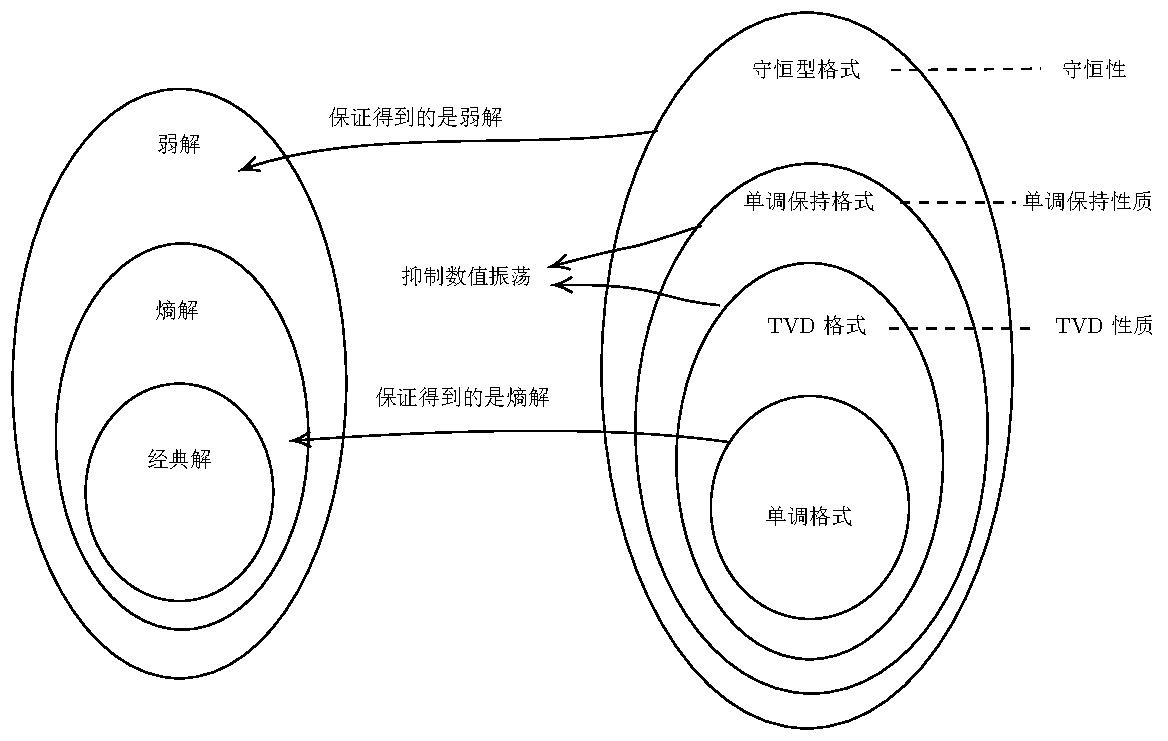
\includegraphics[width=\textwidth]{tikz/cv-schemes.pdf}
    \caption{守恒律方程的各种数值格式与各种解之间的关系} \label{fig:cv-schemes}
\end{figure}


\section{数值格式(二)}

前文中设计的数值格式具有如下特点:
\begin{enumerate}
    \item 基于流通分裂构造的 Lax-Friedrichs 格式是单调格式;
    \item 使用空间平均替换得到的 Lax 格式是单调格式;
    \item 基于 Roe 平均构造的 Roe 迎风格式是TVD格式,但不是单调格式;
    \item 基于时间泰勒展开得到的 Lax-Wendroff 格式是守恒型格式,但不是单调保持格式,可能产生数值振荡。
\end{enumerate}


\begin{example}\label{eg:lax-friedrichs}
    考虑基于流通分裂构造的 Lax-Friedrichs 格式,证明它是 TVD 格式。
\end{example}

\begin{proof}
    {\small
        \begin{align*}
            v_j^{n+1} ={} & v_j^n - \frac{\Delta t}{\Delta x}(f^+(v_{j}^n)-f^+(v_{j-1}^n))
            - \frac{\Delta t}{\Delta x}(f^-(v_{j+1}^n)-f^-(v_{j}^n))                       \\
            ={}           & v_j^n - \frac{\Delta t}{\Delta x}\left(
            f^+(v_{j}^n) + f^-(v_{j+1}^n) - f^+(v_{j-1}^n) - f^-(v_{j}^n)
            \right)                                                                        \\
            ={}           & v_j^n - \frac{\Delta t}{\Delta x}\left(
            \hat{f}_{j+\frac12}^n - \hat{f}_{j-\frac12}^n
            \right)
        \end{align*}}
    因此 Lax-Friedrichs 格式是守恒型格式,对应的数值流通量 $\hat{f}_{j+\frac12} = \hat{f}^{LF}(v_j^n,v_{j+1}^n)$ 称为 Lax-Friedrichs flux,具体定义为
    \[
        \hat{f}^{LF}(u^-,u^+) =
        f^+(u^-) + f^-(u^+) =
        \frac12(f(u^-)+f(u^+)) - \frac{\alpha}2 (u^+-u^-),\quad \alpha = \max |f'| \qedhere
    \]
\end{proof}


\begin{example}
    考虑基于流通分裂构造的 Lax-Friedrichs 格式,在满足 CFL 条件时,证明它是单调格式。
\end{example}

\begin{proof}
    \[
        v_j^{n+1} ={}  v_j^n - \frac{\Delta t}{\Delta x}(f^+(v_{j}^n)-f^+(v_{j-1}^n))
        - \frac{\Delta t}{\Delta x}(f^-(v_{j+1}^n)-f^-(v_{j}^n))   =:   H(v_{j-1}^n,v_j^n,v_{j+1}^n).
    \]
    单调性要求
    \begin{align*}
        \frac{\partial H}{\partial v^n_{j-1}} ={} & \frac{\Delta t}{2\Delta x}(f'(v^n_{j-1})+\alpha)\ge 0 , \\
        \frac{\partial H}{\partial v^n_{j}} ={}   & 1-\alpha\frac{\Delta t}{\Delta x}\ge 0,                 \\
        \frac{\partial H}{\partial v^n_{j+1}} ={} & \frac{\Delta t}{2\Delta x}(\alpha-f'(v^n_{j+1}))\ge  0
    \end{align*}
    $\alpha = \max |f'|$ 可以保证第一个和第三个不等式成立,第二个不等式即 CFL 条件。
\end{proof}

\begin{example}
    考虑使用空间平均替换得到的 Lax 格式,在满足 CFL 条件时,证明它是单调格式。
\end{example}

\begin{proof}
    \[
        v_j^{n+1} = \frac12 (v_{j-1}^n + v_{j+1}^n)
        - \frac{\Delta t}{2\Delta x} \left(f(v_{j+1}^n)-f(v_{j-1}^n)\right)  =:   H(v_{j-1}^n,v_j^n,v_{j+1}^n).
    \]
    单调性要求
    \[
        \frac{\partial H}{\partial v^n_{j-1}} ={}  \frac12(1 + \frac{\Delta t}{\Delta x}f'(v^n_{j-1}))
        \ge 0 ,\quad
        \frac{\partial H}{\partial v^n_{j}} ={}  0       ,\quad
        \frac{\partial H}{\partial v^n_{j+1}} ={} \frac12(1 - \frac{\Delta t}{\Delta x}f'(v^n_{j+1}))
        \ge 0
    \]
    CFL 条件 $\max |f'| \Delta t \le \Delta x$ 可以保证第一个和第三个不等式成立。
\end{proof}


\begin{example}
    对于 Engquist-Osher 格式
    \[
        v_j^{n+1} = v_j^n - \frac{\Delta t}{\Delta x}\left( \hat{f}_{j+\frac12}^n - \hat{f}_{j-\frac12}^n \right)
    \]
    其中的数值流通量 $\hat{f}_{j+\frac12}^n = \hat{f}^{EO}(v_j^n,v_{j+1}^n)$ 定义为
    \[
        \hat{f}^{EO}(u^-,u^+) = \frac{f(u^-) + f(u^+)}2 - \frac12 \int_{u^-}^{u^+} |f'(v)| dv
    \]
    在满足 CFL 条件时,证明它是单调格式。
\end{example}

\begin{proof}
    对数值流通量求导可得
    \begin{align*}
        \partial_1 \hat{f}^{EO}(u^-,u^+) & = \frac{f'(u^-) + |f'(u^-)|}2 \ge 0, \\
        \partial_2 \hat{f}^{EO}(u^-,u^+) & = \frac{f'(u^+) - |f'(u^+)|}2 \le 0.
    \end{align*}
    单调性要求
    \begin{align*}
        \frac{\partial H}{\partial v^n_{j-1}} ={} & \frac{\Delta t}{\Delta x} \partial_1 \hat{f}^{EO}(v_{j-1}^n,v^n_{j}) \ge 0   \\
        \frac{\partial H}{\partial v^n_{j}} ={}   & 1 - \frac{\Delta t}{\Delta x}
        \left[
            \partial_1 \hat{f}^{EO}(v_{j}^n,v^n_{j+1}) - \partial_2 \hat{f}^{EO}(v_{j-1}^n,v^n_{j})
        \right]  = 1 - \frac{\Delta t}{\Delta x} |f'(v_j^n)| \ge 0                                                               \\
        \frac{\partial H}{\partial v^n_{j+1}} ={} & - \frac{\Delta t}{\Delta x} \partial_2 \hat{f}^{EO}(v_{j}^n,v^n_{j+1}) \ge 0
    \end{align*}
    CFL 条件 $\max |f'| \Delta t \le \Delta x$ 可以保证第二个不等式成立。
\end{proof}

\begin{example}
    考虑基于 Roe 平均构造的 Roe 迎风格式,在满足 CFL 条件时,证明它是TVD格式。
\end{example}

\begin{proof}
    {\small
        \begin{align*}
            v_j^{n+1} ={} & v_j^n - \frac{\Delta t}{2\Delta x}
            (1+\text{sgn}(a_{j-\frac12}^n))(f(v_{j}^n)-f(v_{j-1}^n))
            - \frac{\Delta t}{2\Delta x} (1-\text{sgn}(a_{j+\frac12}^n))(f(v_{j+1}^n)-f(v_{j}^n))                                                            \\
            ={}           & v_j^n - \frac{\Delta t}{2\Delta x}
            (1+\text{sgn}(a_{j-\frac12}^n))\frac{f(v_{j}^n)-f(v_{j-1}^n)}{v_{j}^n-v_{j-1}^n}(v_{j}^n-v_{j-1}^n)                                              \\
                          & - \frac{\Delta t}{2\Delta x} (1-\text{sgn}(a_{j+\frac12}^n))\frac{f(v_{j+1}^n)-f(v_{j}^n)}{v_{j+1}^n-v_{j}^n}(v_{j+1}^n-v_{j}^n) \\
            =:{}          & v_j^n - C_{j-\frac12}(v_j^n - v_{j-1}^n) + D_{j+\frac12}(v_{j+1}^n - v_j^n)
        \end{align*}}
    其中
    \begin{align*}
        C_{j-\frac12} & = \frac{\Delta t}{2\Delta x}
        (1+\text{sgn}(a_{j-\frac12}^n))\frac{f(v_{j}^n)-f(v_{j-1}^n)}{v_{j}^n-v_{j-1}^n}
        = \frac{\Delta t}{2\Delta x}
        (1+\text{sgn}(a_{j-\frac12}^n)) a_{j-\frac12}^n \,\ge 0 , \\
        D_{j+\frac12} & = - \frac{\Delta t}{2\Delta x}
        (1-\text{sgn}(a_{j+\frac12}^n))\frac{f(v_{j+1}^n)-f(v_{j}^n)}{v_{j+1}^n-v_{j}^n}
        = -\frac{\Delta t}{2\Delta x}
        (1-\text{sgn}(a_{j+\frac12}^n)) a_{j+\frac12}^n \,\ge 0 ,
    \end{align*}
    并且
    \[
        C_{j+\frac12} + D_{j+\frac12}
        ={}  \frac{\Delta t}{2\Delta x} a_{j+\frac12}^n
        (1+\text{sgn}(a_{j+\frac12}^n)-1+\text{sgn}(a_{j+\frac12}^n))
        ={} \frac{\Delta t}{\Delta x}
        \text{sgn}(a_{j+\frac12}^n)  a_{j+\frac12}^n \le 1
    \]
    对应为 CFL 条件:$\text{max}|a_{j+\frac12}^n| \, \Delta t \le \Delta x$。
\end{proof}

\begin{remark}
    即使在满足 CFL 条件时,Roe 迎风格式也不是单调格式。
\end{remark}


\begin{example}
    Lax-Wendroff 格式是守恒型格式。
\end{example}

\begin{proof}
    \begin{align*}
        v_j^{n+1} ={} & v_j^n
        - \frac{\Delta t}{2\Delta x} \left(f(v_{j+1}^n)-f(v_{j-1}^n)\right)
        \\ & + \frac{\Delta t^2}{2\Delta x^2}\left\{
        A_{j+\frac12}^n [f(v_{j+1}^n) - f(v_{j}^n)]
        - A_{j-\frac12}^n [f(v_{j}^n) - f(v_{j-1}^n)]
        \right\}
        \\
        ={}           & v_j^n - \frac{\Delta t}{\Delta x}
        \Big\{
        \left(\frac12(f(v_j^n)+f(v_{j+1}^n)) - \frac{\Delta t}{2\Delta x} A_{j+\frac12}^n[f(v_{j+1}^n) - f(v_{j}^n)]\right)
        \\ & -
        \left(\frac12(f(v_{j-1}^n)+f(v_{j}^n)) - \frac{\Delta t}{2\Delta x} A_{j-\frac12}^n[f(v_{j}^n) - f(v_{j-1}^n)]\right)
        \Big\}                                                  \\
        =:{}          & v_j^n - \frac{\Delta t}{\Delta x}\left(
        \hat{f}_{j+\frac12}^n - \hat{f}_{j-\frac12}^n
        \right)
    \end{align*}
    因此 Lax-Wendroff 格式是守恒型格式,对应的数值流通量 $\hat{f}_{j+\frac12}$ 为
    \[
        \hat{f}_{j+\frac12} = \frac12(f(v_j^n)+f(v_{j+1}^n)) - \frac{\Delta t}{2\Delta x} A_{j+\frac12}^n[f(v_{j+1}^n) - f(v_{j}^n)] \qedhere
    \]
\end{proof}

\begin{remark}
    数值实验表明,Lax-Wendroff 格式可能产生数值振荡,因此它不是单调保持格式。
\end{remark}


\appendix

\chapter{Fourier基础}

\section{Fourier级数}

\begin{theorem}
    对于以 $2\pi$ 为周期的函数 $f \in C^1(\mathbb{R})$,对应的Fourier级数为
    \[
        S(x) = \frac{1}{\sqrt{2\pi}} \sum_{\omega = -\infty}^\infty \hat{f}(\omega) e^{i \omega x}
    \]
    其中 Fourier 系数为
    \[
        \hat{f}(\omega) = \frac{1}{\sqrt{2\pi}} \int_{0}^{2\pi} f(x)e^{-i \omega x} \,dx
    \]
    那么,Fourier级数 $S(x)$ 一致收敛于 $f(x)$。
\end{theorem}


\begin{theorem}
    对于 $2\pi$ 周期的分片 $C^1$ 函数 $f$,
    若 $f \in C^1((a,b))$,则在任意连续闭区间 $[\alpha,\beta] \subset (a,b)$,
    都有Fourier级数一致收敛于 $f(x)$。
    对于间断点 $x_0$,Fourier 级数收敛于 $\frac12(f(x_0^+) + f(x_0^-))$。
\end{theorem}



\begin{theorem}
    对于 $2\pi$ 周期的分片 $C^1$ 函数 $g(x)$,
    假设 $g$ 的 $p-1$ 阶导数连续,$p$ 阶导数是分片 $C^1$ 的,那么存在常数 $C$,使 $g$ 的Fourier系数满足
    \[
        |\hat{g}(\omega)| \le \frac{C}{|\omega|^{p+1}+1}
    \]
\end{theorem}

考虑内积和对应的 $L^2$ 范数
\[
    (f,g) := \int_0^{2\pi} \overline{f(x)}g(x)\,dx,\,\|f\| := \sqrt{(f,f)}
\]


\begin{lemma}
    指数函数 $\frac{1}{\sqrt{2\pi}} e^{i n x},n=0,\pm 1,\pm 2,\cdots$
    在 $L^2$ 内积下是标准正交的
    \[
        \left(\frac{1}{\sqrt{2\pi}} e^{i m x},\frac{1}{\sqrt{2\pi}} e^{i n x}\right)
        =\, \delta_{mn} =  \left\{
        \begin{aligned}
            0, m \neq n \\
            1, m = n
        \end{aligned}
        \right.\]
\end{lemma}


\begin{theorem}[Parseval 关系]
    对于 $2\pi$ 周期函数 $f,g \in L^2$
    \[
        f(x) = \frac{1}{\sqrt{2\pi}} \sum_{\omega = -\infty}^\infty \hat{f}(\omega) e^{i \omega x},\quad
        g(x) = \frac{1}{\sqrt{2\pi}} \sum_{\omega = -\infty}^\infty \hat{g}(\omega) e^{i \omega x}
    \]
    那么,
    \[
        (f,g) = \sum_{\omega = -\infty}^\infty \overline{\hat{f}(\omega)} \hat{g}(\omega),\quad
        \|f\|^2 = \sum_{\omega = -\infty}^\infty |\hat{f}(\omega)|^2
    \]
\end{theorem}




\begin{theorem}
    对于任意 $2\pi$ 周期函数 $f(x) \in L^2$,Fourier级数部分和在 $L^2$ 意义下收敛到 $f$,即
    \[
        \lim_{N \to \infty} \|f - S_N\| = 0.
    \]
    其中
    \[
        S_N(x) = \frac{1}{\sqrt{2\pi}} \sum_{\omega = -N}^N \hat{f}(\omega) e^{i \omega x},\quad
        \hat{f}(\omega) = \frac{1}{\sqrt{2\pi}} \int_0^{2\pi} e^{-i \omega x}f(x)\,dx.
    \]
\end{theorem}


\section{三角插值}

 {\color{blue}为了记号的方便,只讨论 $N$ 为偶数的情形。} 将 $[0,2\pi]$ 等分为 $N+1$ 个小区间,对应 $N+1$ 个节点:$x_j$, $j = 0,\cdots,N$,记空间步长 $\Delta x = \frac{2\pi}{N+1}$。
对于 $2\pi$ 周期的函数 $u(x)$,记 $u_j = u(x_j)$,
存在唯一的“三角函数”
\[
    \text{Int}_N\,u(x) = \frac{1}{\sqrt{2\pi}} \sum_{\omega = -N/2}^{N/2} \widetilde{u}(\omega) e^{i \omega x}
\]
满足 $\text{Int}_N\,u(x)$ 在 $\{x_j\}_{j=0,\dots,N}$ 插值 $u$,即
\[
    \text{Int}_N\,u(x_j) = \frac{1}{\sqrt{2\pi}} \sum_{\omega = -N/2}^{N/2} \widetilde{u}(\omega) e^{i \omega x_j} = u(x_j),\quad
    j=0,\cdots,N.
\]
下面默认 $u,v$ 均为 $2\pi$ 周期的函数。

\begin{lemma}
    指数函数 $\frac{1}{\sqrt{2\pi}} e^{i n x},n=0,\pm 1,\pm 2,\cdots$
    关于离散 $L^2$ 内积是标准正交的
    \[
        \left(\frac{1}{\sqrt{2\pi}} e^{i m x},\frac{1}{\sqrt{2\pi}} e^{i n x}\right)_{\Delta x}
        =\, \delta_{mn} =
        \begin{cases}
            0, & 0 < |m-n| \le N \\
            1, & m = n
        \end{cases}
    \]
\end{lemma}


\begin{theorem}
    三角插值 $\text{Int}_N\,u(x)$ 存在且唯一,具体表达式为
    \[
        \text{Int}_N\,u(x) = \frac{1}{\sqrt{2\pi}} \sum_{\omega = -N/2}^{N/2} \widetilde{u}(\omega) e^{i \omega x}
    \]
    其中的系数为
    \[
        \widetilde{u}(\omega) = \frac{1}{\sqrt{2\pi}}(e^{i \omega x},u)_{\Delta x},\quad
        |\omega| \le \frac{N}{2}
    \]
\end{theorem}


\begin{theorem}
    考虑对于 $u$ 和 $v$ 的三角插值 $\text{Int}_N\,u(x)$ 和 $\text{Int}_N\,v(x)$
    \[
        \text{Int}_N\,u(x) = \frac{1}{\sqrt{2\pi}} \sum_{\omega = -N/2}^{N/2} \widetilde{u}(\omega) e^{i \omega x},\quad
        \text{Int}_N\,v(x) = \frac{1}{\sqrt{2\pi}} \sum_{\omega = -N/2}^{N/2} \widetilde{v}(\omega) e^{i \omega x}.
    \]
    那么
    \[
        (u,v)_{\Delta x} = \sum_{\omega = -N/2}^{N/2} \overline{\widetilde{u}(\omega)} \widetilde{v}(\omega) = (\text{Int}_N\,u,\text{Int}_N\,v) = (\text{Int}_N\,u,\text{Int}_N\,v)_{\Delta x}.
    \]
    以及
    \[
        \|u\|_{\Delta x}^2 = \sum_{\omega = -N/2}^{N/2} |\widetilde{u}(\omega)|^2 = \|\text{Int}_N\,u\|^2 = \|\text{Int}_N\,u\|_{\Delta x}^2.
    \]
\end{theorem}


\begin{theorem}
    对于 $u(x)$ 和它的三角插值 $\text{Int}_N\,u(x)$,有如下不等式成立
    \[
        \| D^\ell_+\,u\|_{\Delta x}^2 \le
        \left\| \frac{d^\ell}{dx^\ell}\,\text{Int}_N \,u\right\|^2 \le
        \left(\frac{\pi}2\right)^{2\ell} \|D^\ell_+\,u\|_{\Delta x}^2,\quad \ell=1,2,\cdots
    \]
\end{theorem}

考虑 $u$ 的 Fourier 级数和三角插值 $\text{Int}_N\,u$
\[
    u(x) = \frac{1}{\sqrt{2\pi}} \sum_{\omega = -\infty}^\infty \widehat{u}(\omega) e^{i \omega x},\quad
    \text{Int}_N\,u(x) = \frac{1}{\sqrt{2\pi}} \sum_{\omega = -N/2}^{N/2} \widetilde{u}(\omega) e^{i \omega x}
\]
显然 Fourier 系数 $\widehat{u}(\omega)$ 和三角插值系数 $\widetilde{u}(\omega)$ 存在一定的联系。

\begin{lemma}
    Fourier 系数 $\widehat{u}(\omega)$ 和三角插值系数 $\widetilde{u}(\omega)$ 满足如下关系
    \[
        \widetilde{u}(\omega) = \sum_{\ell = -\infty}^\infty \widehat{u}(\omega + \ell(N+1)),\quad |\omega| \le \frac{N}2
    \]
\end{lemma}

特别地,如果对于 $|\omega| > \frac{N}2$ 都有 $\widehat{u}(\omega) = 0$,这表明 $u$ 不含高频部分,三角插值严格等于原函数:$\text{Int}_N\,u(x) = u(x)$,此时 $\widetilde{u}(\omega) = \widehat{u}(\omega)$,$|\omega| \le \frac{N}2$。

\begin{theorem}
    如果 $u$ 的 Fourier 系数满足
    \[
        |\widehat{u}(\omega)| \le \frac{C}{|\omega|^m+1},\quad m > 1
    \]
    那么
    \[
        \|u - \text{Int}_N\,u\|_{\Delta x} \le \frac{2C}{\sqrt{2\pi}}
        \left(\frac{N}2\right)^{1-m}
        \left(
        \frac{1}{m-1} + \frac{2(N+1)}N B_m
        \right)
    \]
    其中 $B_m$ 定义为 $B_m = \sum_{j = 1}^\infty \frac{1}{(2j-1)^m}$。
\end{theorem}

\begin{corollary}
    存在常数 $C_\ell > 0$,使得
    \[
        \left\|
        \frac{d^\ell \,u}{dx^\ell} - \frac{d^\ell \,\text{Int}_N\,u}{d x^\ell}
        \right\|_{\infty}
        \le C_\ell \left(\frac{N}2\right)^{1+\ell-m},\quad 1+\ell < m
    \]
\end{corollary}


\section{基于三角插值的收敛性定理的证明}



\begin{proof}[\normalfont\bfseries Proof of Theorem~\ref{thm:big-thm}]
    % Gustafsson, Bertil《Time Dependent Problems and Difference Methods》 。

    对于固定时刻 $t^n$,我们可以基于数值解 $\{v_j^n\}$ 获取对应时刻的三角插值多项式 $\text{Int}_N\,(v_j^n)$,具体表达式为
    \[
        \text{Int}_N\,(v_j^n)(x)  = \frac{1}{\sqrt{2\pi}} \sum_{\omega = -N/2}^{N/2} e^{i \omega  x} \widehat{Q}^n(\xi) \tilde{f}(\omega )
    \]
    在 $t^n$ 时刻的精确解 $u(x,t^n)$ 可以表示为
    \[
        u(x,t^n) = \frac{1}{\sqrt{2\pi}} \sum_{\omega = -\infty}^{\infty} e^{i \omega (x+t^n)} \hat{f}(\omega )
    \]
    取一个固定的整数 $M$ 使得 $0 < M < N/2$,那么
    {\small
    \begin{align*}
        \| u(\cdot,t^n) - \text{Int}_N\,(v_j^n) \|^2 ={} & \sum_{\omega = -N/2}^{N/2}
        \left| e^{i \omega t^n} \hat{f}(\omega ) - \widehat{Q}^n(\xi) \tilde{f}(\omega ) \right|^2
        + \sum_{|\omega| > N/2} |\hat{f}(\omega)|^2                                                                                                                          \\
        \le{}                                            & \sum_{\omega = -M}^{M} \left| e^{i \omega t^n} \hat{f}(\omega ) - \widehat{Q}^n(\xi) \tilde{f}(\omega ) \right|^2
        + 2 \sum_{|\omega| > M} |\hat{f}(\omega)|^2
        + 2 \sum_{|\omega| > M} |\widehat{Q}^n(\xi)|^2 |\tilde{f}(\omega)|^2
        \\
        =:{}                                             & I + I\!I + I\!I\!I
    \end{align*}}
    验证随着 $M,N \to \infty$,这三项的极限全部为 $0$,即可完成证明。

    $I\!I$ 最容易估计,由条件 (a) 可得
    \[
        \sum_{\omega = -\infty}^{\infty} |\hat{f}(\omega )|^2 < \infty
    \]
    因此
    \[
        \lim_{M \to \infty} I\!I = 2 \lim_{M \to \infty} \sum_{|\omega| > M} |\hat{f}(\omega)|^2 = 0
    \]

    $I\!I\!I$ 的估计依赖于条件 (a) 和 (b):由于
    \[
        \lim_{N \to \infty} \| \text{Int}_N\,f  - f \| = 0,
    \]
    以及
    \[
        \sup_{0 \le t_n \le T} |\widehat{Q}^n| \le K_s,
    \]
    因此
    \[
        \lim_{M \to \infty} I\!I\!I
        = 2 \lim_{M \to \infty} \sum_{|\omega| > M} |\widehat{Q}^n(\xi)|^2 |\tilde{f}(\omega)|^2
        \le
        4 K_s^2  \lim_{M \to \infty} \sum_{|\omega| > M}
        \Big(|\tilde{f}(\omega) - \hat{f}(\omega)|^2 + |\hat{f}(\omega)|^2 \Big) = 0.
    \]

    最后是 $I$ 的估计:对于固定的 $M$,利用条件 (a),(b) 和 (c) 可以得到
    \begin{align*}
        \lim_{N \to \infty} I ={} & \lim_{N \to \infty} \sum_{\omega = -M}^{M} \left| e^{i \omega t^n} \hat{f}(\omega ) - \widehat{Q}^n(\xi) \tilde{f}(\omega ) \right|^2 \\
        \le{}                     & 2 \lim_{N \to \infty} \sum_{\omega = -M}^{M}
        \left\{
        \left| \widehat{Q}^n(\xi) \left(\tilde{f}(\omega) - \hat{f}(\omega) \right) \right|^2
        + \left| \left(e^{i \omega t^n}  - \widehat{Q}^n(\xi)\right) \hat{f}(\omega ) \right|^2
        \right\} = 0
    \end{align*}

    因此,对于任意 $\varepsilon > 0$,可以选取足够大的 $M$ 使得 $I\!I + I\!I\!I < \varepsilon/2$,然后选取足够大的 $N$ 使得 $I < \varepsilon/2$,收敛性证毕。
\end{proof}


\chapter{补充}

\section{数值格式整理}

\subsection*{一维常系数线性对流方程}

考虑方程 $u_t + a u_x = 0$,其中 $a \neq 0$ 为常数,常见的数值格式如下:
\begin{itemize}
    \item 迎风格式(FTFS / FTBS)
          \[
              \frac{v_j^{n+1} - v_j^n}{\Delta t} + a \frac{v_{j+1}^n - v_{j-1}^{n}}{2\Delta x} = \frac{|a|}{2\Delta x} (v_{j+1}^n - 2 v_j^n + v_{j-1}^{n})
          \]
    \item FTCS(反面示例,无条件不稳定)
          \[
              \frac{v_{j}^{n+1} - v_{j}^n}{\Delta t} + a \frac{v_{j+1}^n - v_{j-1}^n}{2\Delta x} = 0
          \]
    \item Lax-Friedrichs 格式
          \begin{gather*}
              \frac{v_j^{n+1}-v_j^n}{\Delta t} + a \frac{v_{j+1}^n-v_{j-1}^n}{2\Delta x} ={} \left(\frac{\Delta x^2}{2\Delta t}\right) \frac{v_{j+1}^n-2 v_j^n+v_{j-1}^n}{\Delta x^2}     \\
              \frac{v_j^{n+1}-\frac12(v_{j-1}^n+v_{j+1}^n)}{\Delta t} + a \frac{v_{j+1}^n-v_{j-1}^n}{2\Delta x} ={} 0
          \end{gather*}
    \item Lax-Wendroff 格式
          \begin{gather*}
              \frac{v_j^{n+1}-v_j^n}{\Delta t} + a \frac{v_{j+1}^n-v_{j-1}^n}{2\Delta x} = \left(\frac{a^2 \Delta t}{2}\right) \frac{v_{j+1}^n-2 v_j^n+v_{j-1}^n}{\Delta x^2} \\
              v_{j}^{n+1} = v_j^n + \Delta t \,(-a)\,\left(\frac{v_{j+1}^n- v_{j-1}^n}{2\Delta x}\right)
              + \frac{\Delta t^2}2\,a^2\,\left(\frac{v_{j+1}^n-2v_{j}^n+v_{j-1}^n}{\Delta x^2}\right)
          \end{gather*}
    \item 蛙跳格式(CTCS)
          \[
              \frac{v_{j}^{n+1} - v_{j}^{n-1}}{2\Delta t} + a \frac{v_{j+1}^n - v_{j-1}^n}{2\Delta x} = 0
          \]
    \item 盒子格式(Wendroff)
          \begin{gather*}
              \frac{\frac12(v_j^{n+1} + v_{j+1}^{n+1}) - \frac12(v_j^n + v_{j+1}^n)}{\Delta t} + a \frac{\frac12(v_{j+1}^n + v_{j+1}^{n+1})-\frac12(v_j^n + v_j^{n+1})}{\Delta x} = 0 \\
              \left(1 - \frac{a \Delta t}{\Delta x}\right)v_j^{n+1} + \left(1 + \frac{a \Delta t}{\Delta x}\right)v_{j+1}^{n+1} =
              \left(1 + \frac{a \Delta t}{\Delta x}\right)v_j^{n} + \left(1 - \frac{a \Delta t}{\Delta x}\right)v_{j+1}^{n}
          \end{gather*}
\end{itemize}


\subsection*{一维常系数线性扩散方程}

考虑方程 $u_t = b u_{xx}$,其中 $b > 0$ 为常数,常见的数值格式如下:
\begin{itemize}
    \item FTCS
          \[
              \frac{v_{j}^{n+1} - v_{j}^n}{\Delta t} = b \frac{v_{j+1}^n - 2v_{j}^n + v_{j-1}^n}{\Delta x^2}
          \]
    \item BTCS
          \[
              \frac{v_{j}^{n+1} - v_{j}^n}{\Delta t} = b \frac{v_{j+1}^{n+1} - 2v_{j}^{n+1} + v_{j-1}^{n+1}}{\Delta x^2}
          \]
    \item Richardson 格式(CTCS,反面示例,无条件不稳定)
          \[
              \frac{v_{j}^{n+1} - v_{j}^{n-1}}{2\Delta t} = b \frac{v_{j+1}^{n} - 2v_{j}^{n} + v_{j-1}^{n}}{\Delta x^2}
          \]
    \item Du Fort-Frankel 格式
          \[
              \frac{v_j^{n+1}-v_{j-1}^n}{2\Delta t} = b \frac{v_{j+1}^n - (v_{j}^{n-1}+v_j^{n+1}) + v_{j-1}^n}{\Delta x^2}
          \]
    \item $\theta$ 格式
          \[
              \frac{v_{j}^{n+1} - v_{j}^n}{\Delta t}
              =
              b \left[
                  \theta \frac{v_{j+1}^{n+1} - 2v_{j}^{n+1} + v_{j-1}^{n+1}}{\Delta x^2}
                  + (1-\theta) \frac{v_{j+1}^n - 2v_{j}^n + v_{j-1}^n}{\Delta x^2}
                  \right]
          \]
    \item Crank-Nicolson 格式:$\theta$ 格式取 $\theta = \frac12$
    \item Douglas 格式:$\theta$ 格式取 $\theta$ 满足
          \[
              \frac{b \Delta t}{\Delta x^2} = \frac{1}{6(1-2\theta)}
          \]
    \item BDF 格式
          \[
              (1+\theta)\frac{v_{j}^{n+1} - v_{j}^{n}}{\Delta t}
              - \theta \frac{v_j^n - v_j^{n-1}}{\Delta t}
              = b \frac{v_{j+1}^{n} - 2v_{j}^{n} + v_{j-1}^{n}}{\Delta x^2}
          \]
    \item Richtmyer 格式:BDF 格式取 $\theta = \frac12$
\end{itemize}

\subsection*{一维常系数线性对流方程的稳定性结论}

在纯初值或周期边界条件下,使用Fourier方法分析 $u_t+au_x=0$ 的几类经典格式的稳定性,结论如下(记 $r = \frac{a\Delta t}{\Delta x} \neq 0$):
按照格式分类:
\begin{itemize}
    \item FTFS:$r(1+r) \le 0$
    \item FTBS:$r(1-r) \ge 0$
    \item BTFS:$r(1-r) \le 0$
    \item BTBS:$r(1+r) \ge 0$
    \item FTCS:无条件不稳定($r^2 \le 0$ 无法成立)
    \item BTCS:无条件稳定($r^2 \ge 0$ 始终成立)
\end{itemize}
按照 $a$ 的正负分类:(只讨论单侧差商格式)
\begin{enumerate}
    \item $a>0$:风向从左往右
          \begin{itemize}
              \item 迎风格式 FTBS 有条件稳定($0< r \le 1$)
              \item 逆风格式 FTFS 不稳定
              \item “隐式迎风格式” BTFS 有条件稳定($r \ge 1$)
              \item “隐式逆风格式” BTBS 无条件稳定
          \end{itemize}
    \item $a<0$:风向从右往左
          \begin{itemize}
              \item 迎风格式 FTFS 有条件稳定($-1 \le r < 0$)
              \item 逆风格式 FTBS 不稳定
              \item “隐式迎风格式” BTBS 有条件稳定($r \le -1$)
              \item “隐式逆风格式” BTFS 无条件稳定
          \end{itemize}
\end{enumerate}


\nocite{*}
\printbibliography[title={参考文献}]

\end{document}
